% make clean all
% make site deploy
%\documentclass[12pt,titlepage]{article}
\documentclass{tufte-book}
%\usepackage[authoryear]{natbib}
\bibliographystyle{genetics}
\usepackage{amsfonts}
\usepackage{amsmath}
\usepackage{amssymb}
\usepackage{graphicx}
\usepackage{rotating}
%\usepackage{marginnote}
\usepackage{color}
%\usepackage{fullpage}
\usepackage{nicefrac}
\usepackage{csvsimple}
%\usepackage[hypertexnames=false]{hyperref}
%\hypersetup{colorlinks=true, urlcolor=blue, citecolor=black, linkcolor=black}
%\usepackage[normalem]{ulem}
\usepackage{tcolorbox}
\newcommand{\gc}[1]{{\em \color{green} #1}}
\newcommand{\sa}[1]{{\color{black} #1}}
\newcommand{\plr}[1]{{\em \color{green} (#1)}}
\newcommand{\E}{\mathbb{E}}
\renewcommand{\P}{\mathbb{P}}
\newcommand{\half}{\tfrac{1}{2}}

\newcommand{\wbar}{\overline{w}}
% New commands added by Simon:
\newcommand{\fis}{F_{\mathrm{IS}}}
\newcommand{\fit}{F_{\mathrm{IT}}}
\newcommand{\fst}{F_{\mathrm{ST}}}
\newcommand{\Wbar}{\overline{W}}

%\newcounter{Question}[section]
%\setcounter{Question}{1}

\newcounter{question}[section]   %%modified from https://www.sharelatex.com/learn/Counters
%\newenvironment{question}[1][]{\refstepcounter{question}\par   \begin{tcolorbox}
 %   \medskip \textbf{Question~\thequestion. #1}\rmfamily}{\medskip} \end{tcolorbox}


\newenvironment{question}[1][]{\refstepcounter{question}\par\medskip
   \textbf{Question~\thequestion. #1} \rmfamily}{\medskip} 

%\newenvironment{question}[1][]{\refstepcounter{question}\par\medskip
%   \textbf{Question~\thequestion. #1} \rmfamily}{\medskip}
 

\definecolor{rev1}{rgb}{1, 0, 0}

\begin{document}

\title{Population Genetics}
\author{Graham Coop}
%  \small $^1$ Department of Evolution and Ecology \& Center for Population Biology,\\
%  \small University of California, Davis.\\
%  \small To whom correspondence should be addressed: \texttt{gmcoop@ucdavis.edu}\\
%  \small This work is licensed under a Creative Commons Attribution 3.0 Unported License.\\
%  \small http://creativecommons.org/licenses/by/3.0/ \\
%  \small i.e. you are free to reuse and remix this work, but please include an attribution to the original.


\date{}
\maketitle

\tableofcontents

\newpage
\chapter{Introduction}
\newthought{Evolution is change over time.} Biological evolution is the change over time in the genetic composition of a population.\cite{DobzhanskyBook} Our population is made up of a set of interbreeding individuals, the genetic composition which is made up of the  genomes that each individual carries.  While at first this definition of evolution seems at odds with the
common textbook view of the evolution of phenotypes (such as the changing shape
of the finch beaks over generations) it is genetic changes that underpin these
phenotypic changes.  \\

The genetic composition of the population can alter due to the death of individuals or the migration of individuals in or out
of the population. If our individuals have different numbers of children, this
also alters the genetic composition of the population in the next generation.
Every new individual born into the population subtly changes the genetic
composition of the population. Their genome is a unique combination of their
parents' genomes, having been shuffled by segregation and recombination during
meioses, and possibly changed by mutation. \\

Population genetics is the study of the genetic composition of natural
populations. It seeks to understand how this composition has been changed over
time by the forces of mutation, recombination, selection, migration, and
genetic drift.  To understand how these forces interact, it is helpful to
develop simple theoretical models to help our intuition. In these notes we will
work through these models and summarize the major areas of population genetic
theory. While these models will seem na\"{\i}ve (and indeed they are) they are
nonetheless incredibly useful and powerful. Throughout the course we will see
that these simple models yield accurate predictions, such that much of our
understanding of the process of evolution is built on these models. We will
also see how these models are incredibly useful for understanding real patterns
we see in the evolution of phenotypes and genomes, such that much of our
analysis of evolution, in a range of areas from human genetics to conservation,
is based on these models. Therefore, population genetics is key to
understanding various applied questions from how medical genetics identifies
the genes involved in disease to how we preserve small populations (such as a
Florida panther) from extinction. 


\begin{quotation}
``Dobzhansky (1951) once defined evolution as 'a change in the genetic
composition of the populations' (p. 16) an epigram that should not be
mistaken for the claim that everything worth saying about evolution is
contained in statements about genes'' -Lewontin \cite{lewontin01} 
\end{quotation}

\newpage
% TODO: standardized equation notation. Is it eqn, Eqn, Eq? (all three are used).



\chapter{Allele and Genotype Frequencies}
 In this chapter we will
work through how the basics of Mendelian genetics play out at the population
level in sexually reproducing organisms.

	Loci and alleles are the basic currency of population genetics--and indeed of
genetics. \marginnote[-1cm]{A
\emph{locus} (plural: \emph{loci}) is a specific spot in the
genome. The term allele was coined by
\href{https://en.wikipedia.org/wiki/Edith_Rebecca_Saunders}{Edith
  Rebecca Saunders} and  William Bateson in 1902 in their paper ``The facts of heredity in the light of Mendel’s discovery'' .} A locus
may be an entire gene, or a single nucleotide base pair such as A-T. At each
locus, there may be multiple genetic variants segregating in the
population---these different genetic variants are known as \emph{alleles}. If
all individuals in the population carry the same allele, we say that the locus
is \emph{monomorphic}; at this locus there is no genetic variability in the
population. If there are multiple alleles in the population at a locus, we say
that this locus is \emph{polymorphic} (this is sometimes referred to
as a segregating site).

\begin{marginfigure}[3cm]
\begin{center}
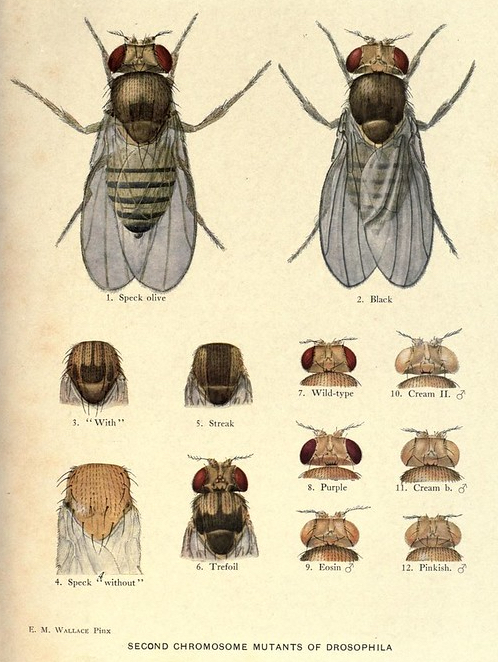
\includegraphics[width= 0.8 \textwidth]{illustration_images/alleles_genotypes/Drosophila_mel/Drosophila_mel_mutants.jpg}
\end{center}
\caption{ {\it Drosophila melanogaster} holds a special place in the
  history of genetics and population genetics. From Morgan's fly room discovering the principals of genetics to Dobzhansky's early work
  on natural genetic variation.  \BHLNC{Contributions to the genetics of Drosophila melanogaster
    (1919). Morgan T.H., Bridges C.B., Sturtevant A. H.}{https://www.biodiversitylibrary.org/page/805594\#page/147/mode/1up}{MBLWHOI Library} } \label{fig:dros}
\end{marginfigure}



Table \ref{Table:ADH} shows a small stretch of orthologous sequence for
the ADH locus from samples from {\it Drosophila melanogaster},  {\it D. simulans},
and {\it D. yakuba}.  {\it D. melanogaster} and {\it D. simulans} are
sister species and  {\it D. yakuba} is a close outgroup to the two.  Each column represents a single haplotype from an
individual (the individuals are diploid but were inbred so they're
homozygous for their haplotype). Only sites that differ among
individuals of the three species are shown. Site $834$ is an example
of a polymorphism; some  {\it D. simulans} individuals carry a $C$
allele while others have a $T$. \emph{Fixed differences}  are sites that differ between the species but are monomorphic within
  the species. Site $781$ is an example of a fixed difference between
  {\it D. melanogaster} and the other two species.

We can also annotate the alleles and loci in various ways. For example, position
$781$ is a non-synonymous fixed difference. We call the less common
allele at a polymorphism the  \emph{minor allele} and the common
allele the \emph{major allele}, e.g. at site $1068$ the $T$ allele is the
minor allele in {\it D. melanogaster}. We call the more evolutionarily
recent of the two alleles the \emph{derived allele} and the older of
the two the \emph{ancestral allele}. We infer that the $T$ allele at site 1068 is
the derived allele because the $C$ is found in both other species,
suggesting that the $T$ allele arose via a $C \rightarrow T$ mutation.

% For example, at a particular nucleotide site in the genome, a population may segregate for A-T and G-C base pairs (note that due to the complementary nature of DNA, it will suffice to say the site segregates for A and G variants).

\begin{table*}
  \tiny
\setlength{\tabcolsep}{.45\tabcolsep}   % https://tex.stackexchange.com/questions/307770/centered-tabular-column-with-narrow-columns
 %\csvreader[tabular=c]{Journal_figs/alleles_genotypes/ADH_MK/ADH.csv}
\csvautobooktabular{Journal_figs/alleles_genotypes/ADH_MK/ADH.csv}  % can control this more https://mirror.hmc.edu/ctan/macros/latex/contrib/csvsimple/csvsimple.pdf
  \caption{Variable sites in exons 2 and 3 of the ADH gene in {\it Drosophila} \citet{mcdonald:91}.
The first column (pos.) gives the position in the gene; exon 2 begins at
position $778$ and we've truncated the dataset at site $1175$.
The second column gives the consensus nucleotide (con.), i.e. the most
common base at that position; individuals with nucleotides that match
the consensus are marked with a dash.  The first columns of sequence
(a-l) are from {\it D. melanogaster};
    the next columns (a-f) give sequences from \textit{D. simulans}, and the final
 set of columns (a-l ) from {\it D. yakuba}. The last column shows
 whether the difference is a non-synonymous (N) or synonymous (S) change. }  % I've dropped the
                                % heterozygote sites from D. yakuba.
  \label{Table:ADH}
\end{table*}

\begin{question}
{\bf A)} How many segregating sites does the sample from \textit{
  D. simulans} have in the ADH gene?\\
{\bf B)} How many fixed differences are there between \textit{D. melanogaster} and \textit{D. yakuba}?
%What is the per base divergence are there between {\emph D. melanogaster} and {\emph D. yakuba}?
\end{question}
%JRI: confusing because site 974 is tri-allelic so "fixed" for derived allele but...

\section{Allele frequencies}
Allele frequencies are a central unit of population genetics
analysis, but from diploid individuals we only get to observe genotype
counts. Our first task then is to calculate allele frequencies from
genotype counts. Consider a diploid autosomal locus segregating for two alleles ($A_1$ and
$A_2$). We'll use these arbitrary labels for our alleles, merely to keep this
general. Let $N_{11}$ and $N_{12}$ be the number of $A_1A_1$ homozygotes and
$A_1A_2$ heterozygotes, respectively. Moreover, let $N$ be the total number of
diploid individuals in the population. We can then define the relative
frequencies of $A_1A_1$ and $A_1A_2$ genotypes as $f_{11} = N_{11}/N$ and
$f_{12} = N_{12}/N$, respectively. The frequency of allele $A_1$ in the
population is then given by

\begin{equation}
  p = \frac{2 N_{11} + N_{12}}{2N} = f_{11} + \frac{1}{2} f_{12}.
\end{equation}
Note that this follows directly from how we count alleles given individuals'
genotypes, and holds independently of Hardy--Weinberg proportions and
equilibrium (discussed below). The frequency of the alternate allele ($A_2$) is
then just $q=1-p$.

\subsection{Measures of genetic variability}
\paragraph{Nucleotide diversity ($\pi$)}
One common measure of genetic diversity is the average number of single
nucleotide differences between haplotypes chosen at random from a
sample. This is called \emph{nucleotide diversity} and is often denoted by
$\pi$.
For example, we can calculate $\pi$ for our ADH locus from Table \ref{Table:ADH} above: we have
6 sequences from \textit{D. simulans}  (a-f), there's a total of 15 ways of pairing
these sequences, and
\begin{equation}
\pi=\frac{1}{15} \big( (2 + 1 + 1 + 1 + 0 ) + (3 + 3 + 3 + 2 ) +(0 + 0 + 1) + (0 + 1) + (1)  \big)=1.2\overline{6}
\end{equation}
where the first bracketed term gives the pairwise differences between
a and b-f, the second bracketed term the differences between b and c-f
and so on. \\

Our $\pi$ measure will depend on the length of sequence it is calculated
for. Therefore, $\pi$ is usually normalized by the length of sequence,
to be a per site (or per base) measure. For example, our ADH sequence covers $397$bp of DNA and so $\pi = 1.2\overline{6}/397=0.0032$ per site in \textit{D. simulans} for this region. Note that we could also calculate $\pi$ per synonymous site (or non-synonymous). For synonymous site $\pi$, we would count up number of synonymous differences between our pairs of sequences, and then divide by the total number of sites where a synonymous change could have occurred.{\sidenote{Technically we would need to divide by the total number of possible point mutations that would result in a synonymous change; this is because some mutational changes at a particular nucleotide will result in a non-synonymous or synonymous change depending on the base-pair change.}


\paragraph{Number of segregating sites.} Another measure of genetic variability is the total number of sites
that are polymorphic (segregating) in our sample. One issue is that
the number of segregating sites will grow as we sequence more
individuals (unlike $\pi$). Later in the course, we'll talk about how to standardize the
number of segregating sites for the number of individuals sequenced (see eqn \eqref{watterson_theta}).

\paragraph{The frequency spectrum.}
We also often want to compile information about the frequency of
alleles across sites.  We call alleles that are found once in a sample
\emph{singletons}, alleles that are found twice in a sample {\emph
  doubletons}, and so on. We count up the number of loci where an
allele is found $i$ times out of $n$, e.g. how many singletons are
there in the sample, and this is called the \emph{frequency
  spectrum}. We'll want to do this in some consistent manner, such as calculating the frequency spectrum of the minor allele or the derived allele.

\begin{question}
How many minor-allele singletons are there in \textit{D. simulans} in
the ADH region? [Defining minor allele just within \textit{D. simulans}.]
%JRI: ambiguous. is the minor allele defined across all species or just within simulans?
\erin{students were confused whether you are defining 'minor allele' with reference to the species or to the whole group. There are no major allele singletons with reference to the individual species, but I think it's confusing because the only example of a minor allele given in the text by its definition is the 'minor allele in D. melanogaster' .. maybe it would be best to clarify in the question or just give an example of the minor allele in the whole sample instead.}
 \end{question}
\paragraph{Levels of genetic variability across species.}
Two observations have puzzled population geneticists since the
inception of molecular population genetics. The first is the relatively high
level of genetic variation observed in most obligately sexual species.
This first observation, in part, drove the development of the Neutral
theory of molecular evolution, the idea that much of this molecular
polymorphism may simply reflect a balance between genetic drift and
mutation.
The second observation is the relatively narrow range of
polymorphism across species with vastly different census sizes. This
observation represented a puzzle as the Neutral theory predicts that
levels of genetic diversity should scale with population size. Much effort
in theoretical and empirical population genetics has been devoted to
trying to reconcile models with these various observations. We'll
return to discuss these ideas throughout our course.
%Neutral

\begin{marginfigure}[-1cm]
\begin{center}
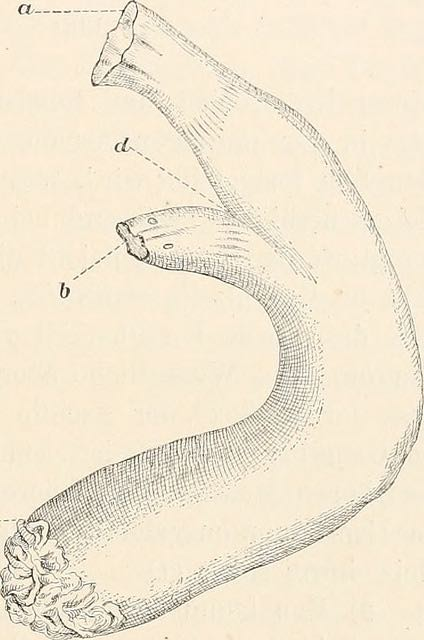
\includegraphics[width= 0.8 \textwidth]{illustration_images/alleles_genotypes/Ciona_intestinalis/21016139168_2a8a57ded3_z.jpg}
\end{center}
\caption{Sea Squirt ({\it Ciona intestinalis}). \BHLNKC{Einleitung in die vergleichende gehirnphysiologie und
  Vergleichende psychologie. Loeb, J. 1899.}{https://www.flickr.com/photos/internetarchivebookimages/21016139168/in/photolist-y28cZ3-xatkQu-w6Ki9C-wLcTJy-tLanR7-wKRZbh-w79C6u-toKNq1-u3ojn3-y8KsPP-xK7CZj-bu2usR-wLkfdM-wbkfau-x8n51o-ygpRAN-xMgGnk-towSTe-xQtix3-xMrift-wQoMNq-y51RxU-xPH4Cu-x4uB1v-xPGVFs-x4GN5a-y6rT8N-y6Aous-y7jV9n-yb6s66-x7F6Wh-y7upRp-xkz9VY-u1qerd-wYE4Cz-y5aH2Y-y7uJpM-xPSvFU-y6ALo7-xPZ3FM-xPHUef-yaa3dw-xPSKSC-w7A1aj-x4bgsH-tLas4q-x1e1dv-w7BkZB-xrQxFJ-y8acDr}{MBLWHOI Library}} \label{fig:ciona}
\end{marginfigure}

The first observations of molecular genetic diversity within natural populations were made from surveys of allozyme data, but we can revisit these general patterns with modern data. \\
\begin{figure*}
\begin{center}
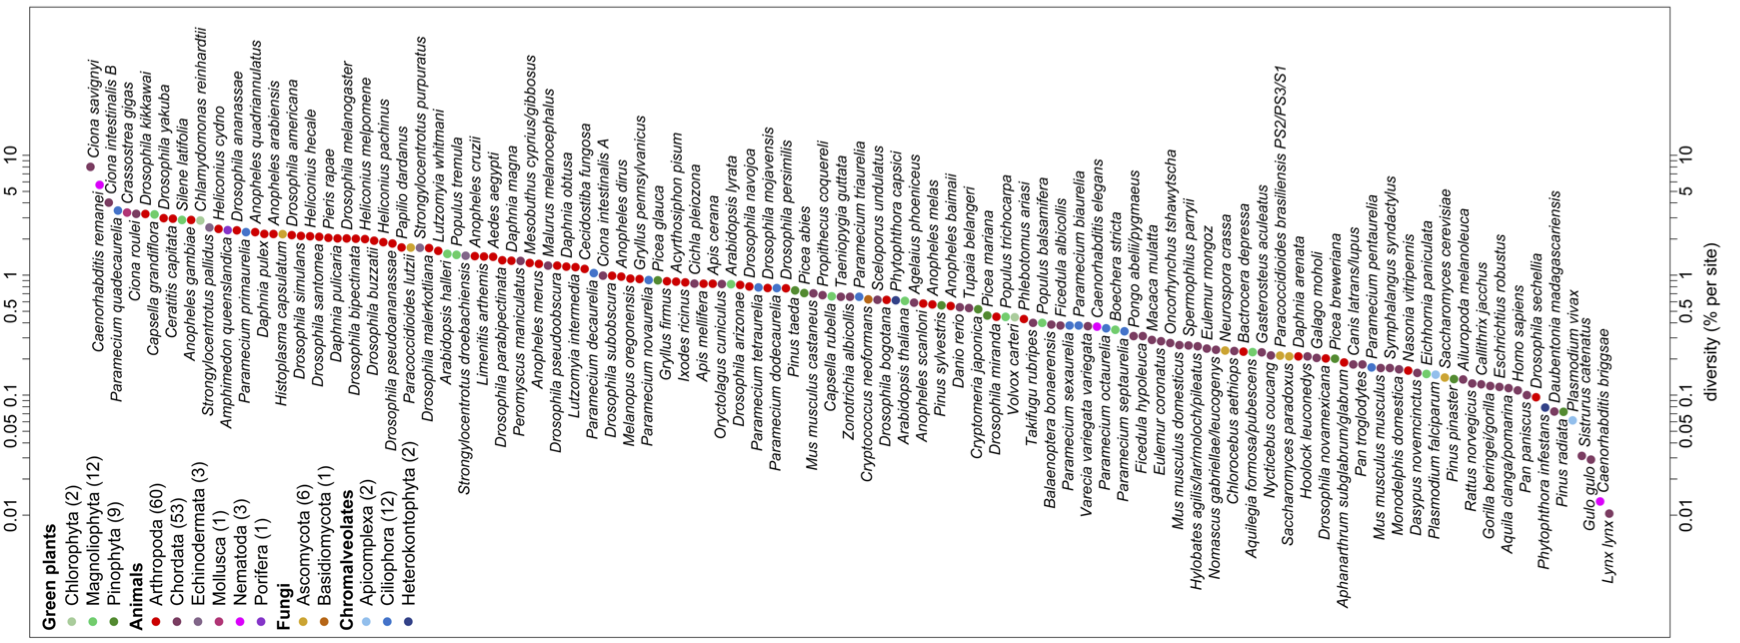
\includegraphics[width= \textwidth]{Journal_figs/alleles_genotypes/Leffer_riddle/Leffer_riddle_diversity.png}
\end{center}
\caption{Levels of autosomal nucleotide diversity for 167
species across 14 phyla. Figure 1 from \citet{leffler:12}, \PLOSccBY. Points are
ranked by their $\pi$, and coloured by their phylum. Note the log-scale.} \label{fig:Leffer}
\end{figure*}
For
example, \citet{leffler:12} compiled data on levels of within-population,
autosomal nucleotide diversity ($\pi$) for 167 species across 14 phyla from
non-coding and synonymous sites (Figure \ref{fig:Leffer}). The species with the lowest levels of
$\pi$ in their survey was Lynx, with $\pi = 0.01\%$, i.e. only
$1/10000$ bases differed between two sequences. In contrast, some of the highest levels of
diversity were found in {\textit{Ciona savignyi}, Sea Squirts, where a remarkable
$1/12$ bases differ between pairs of sequences. This $800$-fold range of
diversity seems impressive, but census population sizes have a much
larger range.
%JRI: I feel like an example of census size would be useful. the genus Cyclothone, which exists in the trillions, comes to mind as a surprising example that you could compare to like a coelocanth: https://commons.wikimedia.org/wiki/File:Wissenschaftliche_Ergebnisse_der_Deutschen_Tiefsee-Expedition_auf_dem_Dampfer_%22Valdivia%22_1898-1899_(Tafel_6)_(7413855904).jpg

\begin{marginfigure}[2cm]
\begin{center}
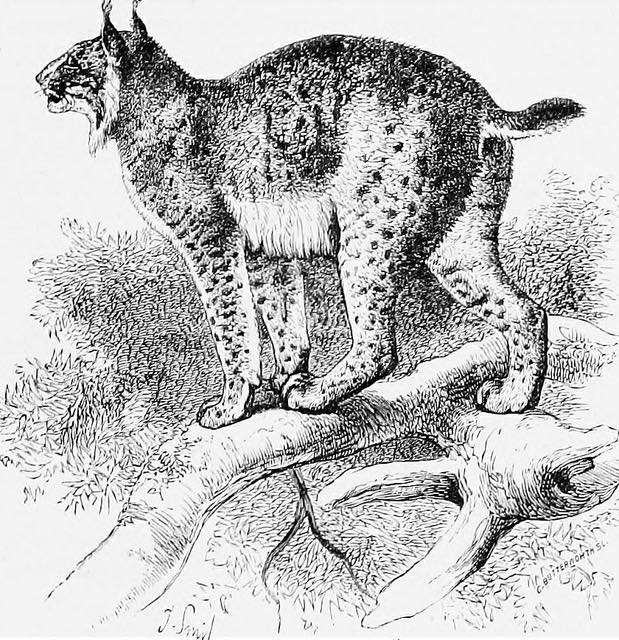
\includegraphics[width= 0.8 \textwidth]{illustration_images/alleles_genotypes/Lynx/20731949565_8a065700af_z.jpg}
\end{center}
\caption{Eurasian Lynx (\textit{Lynx lynx}). \BHLNKC{An introduction to the study
  of mammals living and extinct. Flower, W.H. and Lydekker, R. 1891.}{https://www.flickr.com/photos/internetarchivebookimages/20731949565/in/photolist-x5Jzv2-x6QVyp-xir9rH-wYHrQD-wPn1sP-w9PsqY-xDcqri-sMcQoB-trrkVd-x6Nx1H-wPea7N-sM28N9-tJ3zsp-xneVdx-wGJRtQ-xnfHZ8-wPfga7-xCUPrN-x7kXDV-xmAb9E-xm3x4k-xBoSKb-wGTgyB-xBoSbf-wGGvzA-xmzYTJ-oeKJcH-xA1Ffr-xA1Eji-xqWTQZ-xF4Lru-oxJfrH-x7ojSn-xra8zP-wGGibY-xgb21y-xY1jH9-xY1iyf-wGHxTS-wGQEoR-xmtPQh-x8uFKK-xdTkoU-wPggQf-wPfvHN-wPfc27-w9YnGF-wPeauS-wPiVxK-w6aiSi}{Cornell University Library}} \label{fig:Lynx}
\end{marginfigure}

\subsection{Hardy--Weinberg proportions}
Imagine a population mating at random with respect to genotypes, i.e. no
inbreeding, no assortative mating, no population structure, and no sex differences
in allele frequencies. The frequency of allele $A_1$ in the population at the
time of reproduction is $p$. An $A_1A_1$ genotype is made by reaching out into
our population and independently drawing two $A_1$ allele gametes to form a
zygote. Therefore, the probability that an individual is an $A_1A_1$ homozygote
is $p^2$. This probability is also the expected frequencies of the $A_1A_1$
homozygote in the population. The expected frequency of the three possible
genotypes are

\marginnote{Throughout this chapter we'll be making use of the basic
  rules of probability to find the probabilities of combinations of
  events, e.g. the alleles found in an individual, see Appendix \ref{Section_rules_prob} for a refresher.}

%\begin{table}[htp!]
\begin{center}
\begin{tabular}{ccc}
\hline
$f_{11}$ & $f_{12}$ & $f_{22}$ \\
\hline
$p^2$ & $2pq$ & $q^2$ \\
\end{tabular}
\end{center}
%\caption{\textbf{Hardy Weinberg}} \label{table:HWE}
%\end{table}
Note that we only need to assume random mating with respect to our focal allele in order for these expected frequencies to hold in the zygotes forming the next generation. Evolutionary forces, such as selection, change allele frequencies within generations, but do not change this expectation for new zygotes, as long as $p$ is the frequency of the $A_1$ allele in the population at the time when gametes fuse.
%\erin{I wasn't sure what contrast you were getting at here, so may not be a good edit}

\begin{question}
On the coastal islands of British Columbia there is a subspecies of
black bear (\textit{Ursus americanus kermodei}, Kermode's bear). Many members of this
black bear subspecies are white; they're sometimes called spirit bears. These
bears aren't hybrids with polar bears, nor are they albinos. They are
homozygotes for a recessive change at the MC1R gene. Individuals who
are $GG$ at this SNP are white while $AA$ and $AG$ individuals are black.



\begin{marginfigure}    %%%New Kermode_bear
                        %%%https://twitter.com/BioDivLibrary/status/1191354772034592774/photo/3
                        %%%page 77 https://www.biodiversitylibrary.org/item/38166?utm_source=Twitter&utm_medium=social+media&utm_term=&utm_content=MBLWHOI&utm_campaign=Mammal+Monday#page/114/mode/1up
  \begin{center}
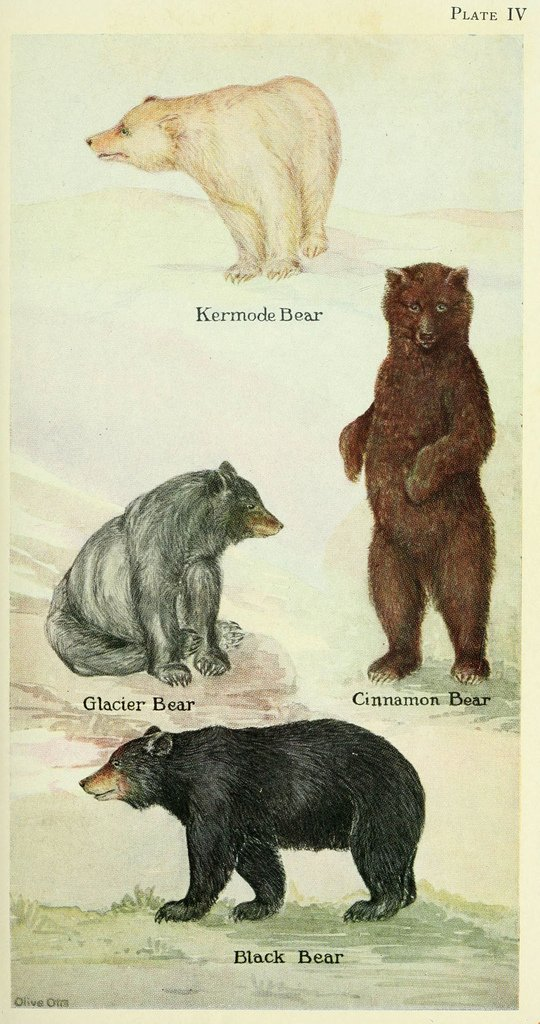
\includegraphics[width= \textwidth]{illustration_images/alleles_genotypes/Kermode_bear/EIiK2dsWoAAmUOf.jpeg}  
%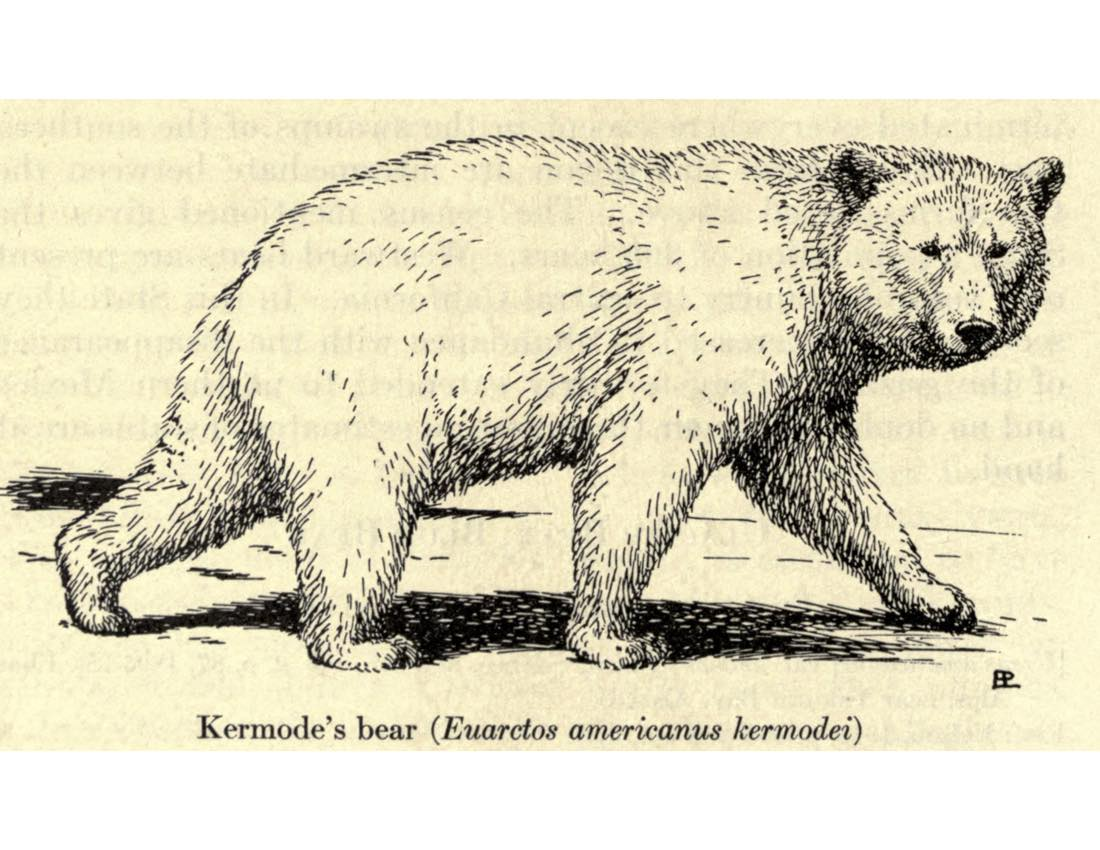
\includegraphics[width= \textwidth]{illustration_images/alleles_genotypes/Kermode_bear/Kermode_bear.jpg}
\end{center}
\caption{Kermode's bear (\textit{Ursus americanus kermodei}). It's
  possible that this morph is favoured as the salmon these bears eat have a harder time
  seeing the light morph \citep{klinka2009adaptive}. The adaptive
  value of tasting like cinnamon is unknown. \BHLNKC{Field book of North American mammals;
    descriptions of every mammal known north of the Rio
    Grande. Anthony, (1928) H. E.}{https://www.biodiversitylibrary.org/item/38166\#page/115/mode/1up}{MBLWHOI Library} } \label{fig:Kermodes_bear}
%\caption{Kermode's bear. \BHLNC{Extinct and vanishing mammals of the western
 % hemisphere. 1942. Glover A.}{https://www.biodiversitylibrary.org/page/20699033\#page/160/mode/1up}{Prelinger
%  Library} } \label{fig:Kermodes_bear}
\end{marginfigure}

Below are the genotype counts for the MC1R polymorphism in a
sample of bears from British Columbia's island populations from \citet{RITLAND:01}.
\begin{center}
\begin{tabular}{ccc}
\hline
$AA$ & $AG$ & $GG$ \\
\hline
42 & 24 & 21\\
\end{tabular}
\end{center}
What are the expected frequencies of the three genotypes under HWE?
\end{question}
%JRI: I think you mean under HW not HWE.  i think somewhere you should introduce HW in a parenthetical"Hard--Weinberg  (HW) proportions" etc. just to be abdunantly clear what the acronym means. also the ritland citation isn't showing year for some reason.


See Figure \ref{fig:HWE_CEU_YRI} for a nice
empirical demonstration of Hardy--Weinberg proportions. The mean
frequency of each genotype
closely matches its HW expectations, and much of the scatter of the
dots around the expected line is due to our small sample size ($\sim
60$ individuals). While HW often
seems like a silly model, it often holds remarkably well within
populations. This is because individuals don't mate at random, but they
do mate at random with respect to their genotype at most of the loci
in the genome.

\begin{figure}[!h]
\begin{center}
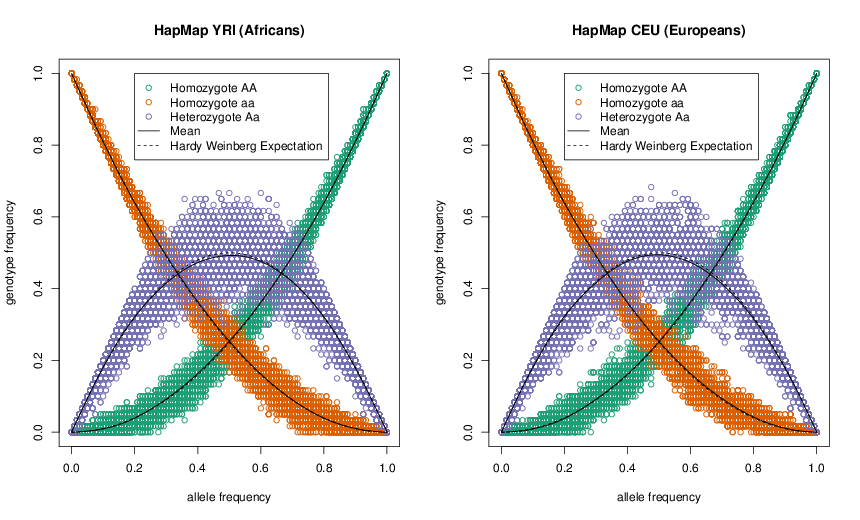
\includegraphics[width= \textwidth]{figures/CEU_YRI_separately_HWE.png}
\end{center}
\caption{Demonstrating Hardy--Weinberg proportions using 10,000 SNPs
  from the HapMap European (CEU)  and African (YRI) populations. Within
  each of these populations the allele frequency against the
  frequency of the 3 genotypes; each SNP is represented by 3 different
  coloured points. The solid lines show the mean genotype frequency. The dashed lines show the
  predicted genotype frequency from Hardy--Weinberg
  equilibrium. \gitcode{https://github.com/cooplab/popgen-notes/blob/master/Rcode/HWE_exercise/HWE_HAPMAP.R} Blog
  post on figure \href{http://gcbias.org/2011/10/13/population-genetics-course-resources-Hardy--Weinberg-eq/}{here}. } \label{fig:HWE_CEU_YRI}  %See \href{blog
                                %post}{http://gcbias.org/2011/10/13/population-genetics-course-resources-Hardy--Weinberg-eq/}
                                %here on this plot.  https://github.com/cooplab/popgen-notes/blob/master/Rcode/HWE_exercise/HWE_HAPMAP.R
\end{figure}

\begin{question}
You are investigating a locus with three alleles, A, B, and C, with
allele frequencies $p_A$, $p_B$, and $p_C$. What fraction of the
population is expected to be homozygotes under Hardy--Weinberg?
\end{question}

Microsatellites are regions of the genome where individuals vary for
the number of copies of some short DNA repeat that they carry. These
regions are often highly variable across individuals, making them
a suitable way to identify individuals from a DNA sample. This
so-called DNA fingerprinting has a range of applications from
establishing paternity and identifying human remains to matching
individuals to DNA samples from a crime scene. The FBI make use of the
CODIS database\sidenote{CODIS: Combined DNA Index System}. The CODIS
database contains the genotypes of over 13 million people, most of
whom have been convicted of a crime. Most of
the profiles record genotypes at 13 microsatellite loci that are
tetranucleotide repeats (since 2017, 20 sites have been genotyped).

The allele counts for two loci (D16S539
and TH01) are shown in table \ref{table:CODIS_1} and
\ref{table:CODIS_2} for a sample of 155 people of European ancestry. You can assume these two loci are on different chromosomes.

\begin{table}
{\small
\setlength{\tabcolsep}{.45\tabcolsep}
\csvautobooktabular{Rcode/CODIS/D16S539_counts.csv}  \label{table:CODIS_1}
\caption{ Data for 155 Europeans at the D16S539 microsatellite from
  CODIS from \citet{algee:16}. The top row gives the number of
  tetranucleotide repeats for each allele, the bottom row gives the
  sample counts.}
 }

\end{table}
\vspace*{1cm}
\begin{table}
  {\small
\setlength{\tabcolsep}{.45\tabcolsep}
\csvautobooktabular{Rcode/CODIS/TH01_counts.csv}  \label{table:CODIS_2}
}

\caption{Same as \ref{table:CODIS_1} but for the TH01 microsatellite. }
\end{table}

\begin{question} \label{Q:CODIS}
You extract a DNA sample from a crime scene. The genotype is 100/80 at the
D16S539 locus and 70/93 at TH01.\\

{\bf A)} You have a suspect in custody. Assuming this suspect is innocent and of European ancestry, what is the probability
that their genotype would match this profile by chance (a false-match probability)?\\
{\bf B)} The FBI uses $\geq 13$ markers. Why is this higher number
necessary to make the match statement convincing evidence in court?\\
{\bf C)}  An early case that triggered debate among forensic geneticists was a crime among the Abenaki, a Native American community in
Vermont \citep[see ][ for discussion]{lewontin:94}. There was a DNA sample from the crime scene, and the
perpetrator was thought likely to be a member of the Abenaki
community. Given that allele frequencies vary among populations, why would people be concerned about using data from a non-Abenaki population to compute a false match probability?
%---that is, the probability
%that a suspect's DNA would match a crime-scene sample if he were unrelated to anyone present at the crime scene
\end{question}

%\begin{question}
%Suppose the following genotype frequencies were observed for at an esterase locus in a population of Drosophila (A denotes the “fast” allele and B denotes the “slow” allele):
%\begin{center}
%\begin{tabular}{|ccc|}
%AA &	AB &	BB\\
%0.6 &	0.2 &	0.2\\
%\end{tabular}\,.
%\end{center}
%What genotype frequencies would you expect under Hardy Weinberg expectations?
%\end{question}


%%%ADD A comment about WF sampling here!
%% Also add a question about Poisson offspring number.

%\begin{figure}
%\begin{center}
%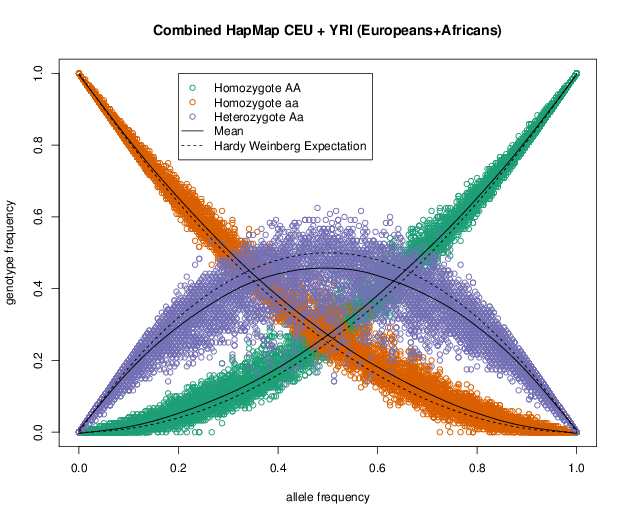
\includegraphics[width=0.5 \textwidth]{figures/CEU_YRI_together_HWE.png}
%\end{center}
%\caption{}
%\end{figure}


%figure/QT1.eps

\section{Allele sharing among related individuals and Identity by Descent}

All of the individuals in a population are related to each other by a giant
pedigree (family tree). For most pairs of individuals in a population these
relationships are very distant (e.g. distant cousins), while some individuals
will be more closely related (e.g. sibling/first cousins). All individuals
are related to one another by varying levels of relatedness, or \emph{kinship}.
Related individuals can share alleles that have both descended from the shared
common ancestor. To be shared, these alleles must be inherited through all
meioses connecting the two individuals (e.g. surviving the $\nicefrac{1}{2}$
probability of segregation each meiosis). As closer relatives are separated by
fewer meioses, closer relatives share more alleles. In Figure
\ref{fig:IBD_cousins_chr_cartoon} we show the sharing of chromosomal regions
between two cousins. As we'll see, many population and quantitative genetic
concepts rely on how closely related individuals are, and thus we need some way
to quantify the degree of kinship among individuals. \\
\begin{figure}
\begin{center}
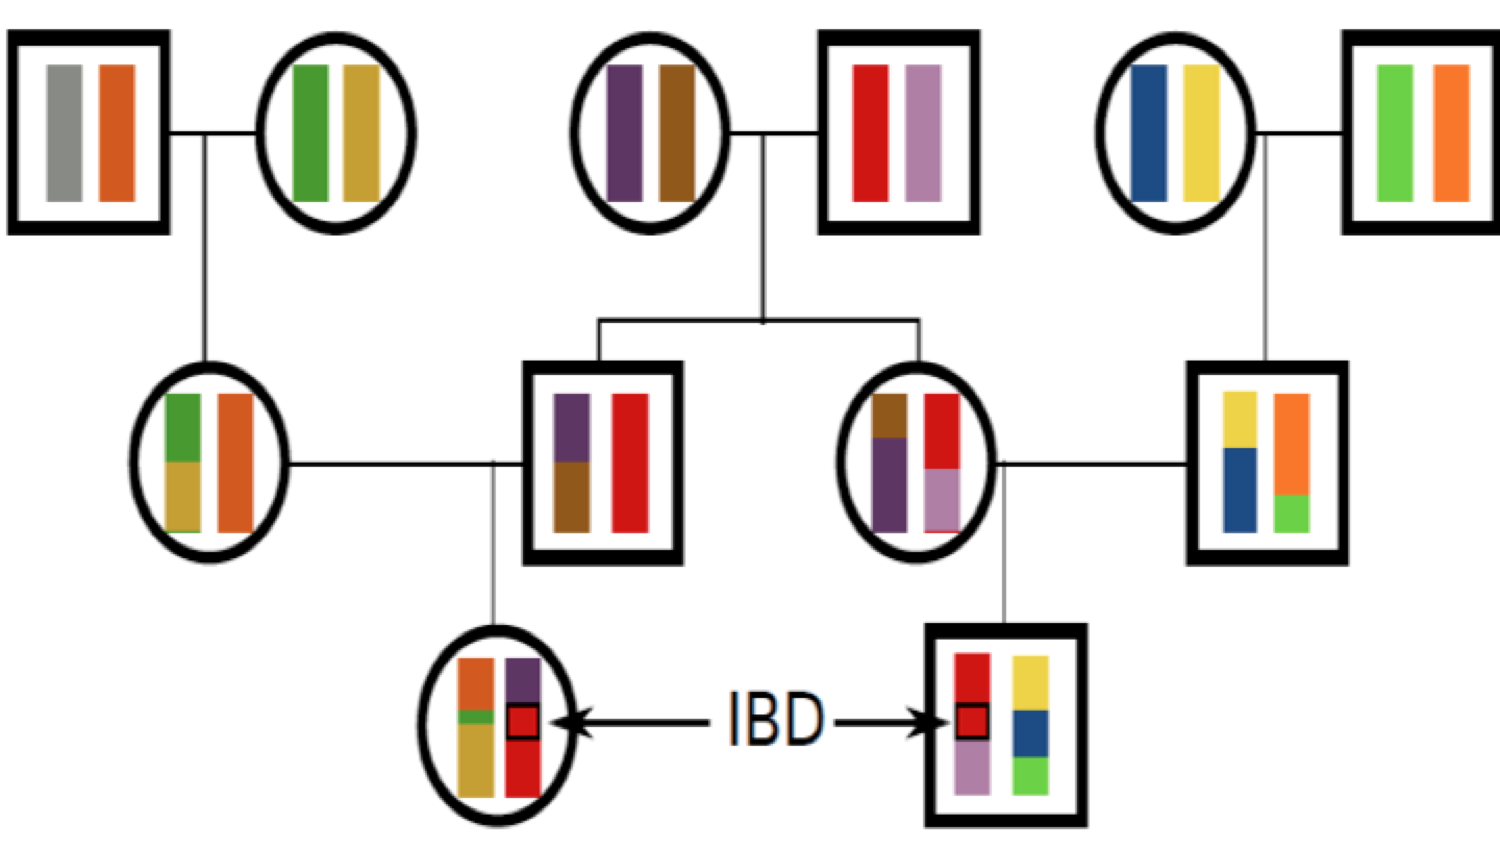
\includegraphics[width= 0.75 \textwidth]{figures/Cousins_IBD_chromo_cartoon.png}
\end{center}
\caption{First cousins sharing a stretch of chromosome identical by
  descent. The different grandparental diploid chromosomes are coloured so we
  can track them and recombinations between them across the
  generations. Notice that the identity by descent between the cousins persists for a long
stretch of chromosome due to the limited number of generations for
recombination. The squares represent males and circles females. } \label{fig:IBD_cousins_chr_cartoon}
\end{figure}

We will define two alleles to be identical by descent (IBD) if they are
identical due to transmission from a common ancestor in the past few generations\cite{cotterman:40,malecot:48}. For the moment,
we ignore mutation, and we will be more precise about what we mean by `past few
generations' later on. For example, parent and child share exactly one allele
identical by descent at a locus, assuming that the two parents of the child are
randomly mated individuals from the population. In Figure
\ref{fig:IBD_cousins_cartoon}, I show a pedigree demonstrating some
configurations of IBD. \\

\marginnote{Here we'll focus on IBD of outbred individuals. Dealing
  with sharing between inbred individuals requires $6$ more  identity-by-descent
$r$ coefficients, which honestly makes my head spin.}
One summary of how related two individuals are is the probability that our pair
of individuals share 0, 1, or 2 alleles identical by descent (see Figure
\ref{fig:IBD_0_1_2}). We denote these  identity-by-descent probabilities by $r_0$, $r_1$, and $r_2$
respectively. See Table \ref{table:IBDprobs} for some examples. We can also
interpret these probabilities as genome-wide averages. For example, on average, at a quarter of all their autosomal loci
full-sibs share zero alleles identical by descent.\\



One summary of relatedness that will be important is the probability that two
alleles ($I$ \& $J$) picked at random, one from each of the two different individuals $i$
and $j$, are identical by descent ($P(\text{I\&J IBD})$). We call this quantity the \emph{coefficient
of kinship} of individuals $i$ and $j$, and denote it by $F_{ij}$. It is
calculated as
%JRI: you come back to inbreeding later, but perhaps worth mentioning here that you are only considering outbred Individuals

\begin{align}
  F_{ij} = & P(\text{I\&J IBD} )\\
  =& P(\text{I\&J IBD} |~ \text{i\&j  0 IBD}) P(\text{i\&j  0 IBD})  \nonumber\\
  & + P(\text{I\&J IBD} |~ \text{i\&j  1 IBD})
    P(\text{i\&j  1 IBD})  \nonumber\\
  &+ P(\text{I\&J IBD} |~ \text{i\&j  2 IBD}) P(\text{i\&j  2 IBD}) \label{eqn:coeffkinship_step}\\
   =   &   0 \times r_0 + \frac{1}{4} r_1  + \frac{1}{2} r_2.
\label{eqn:coeffkinship}
\end{align}
\begin{marginfigure}[-1cm]
\begin{center}
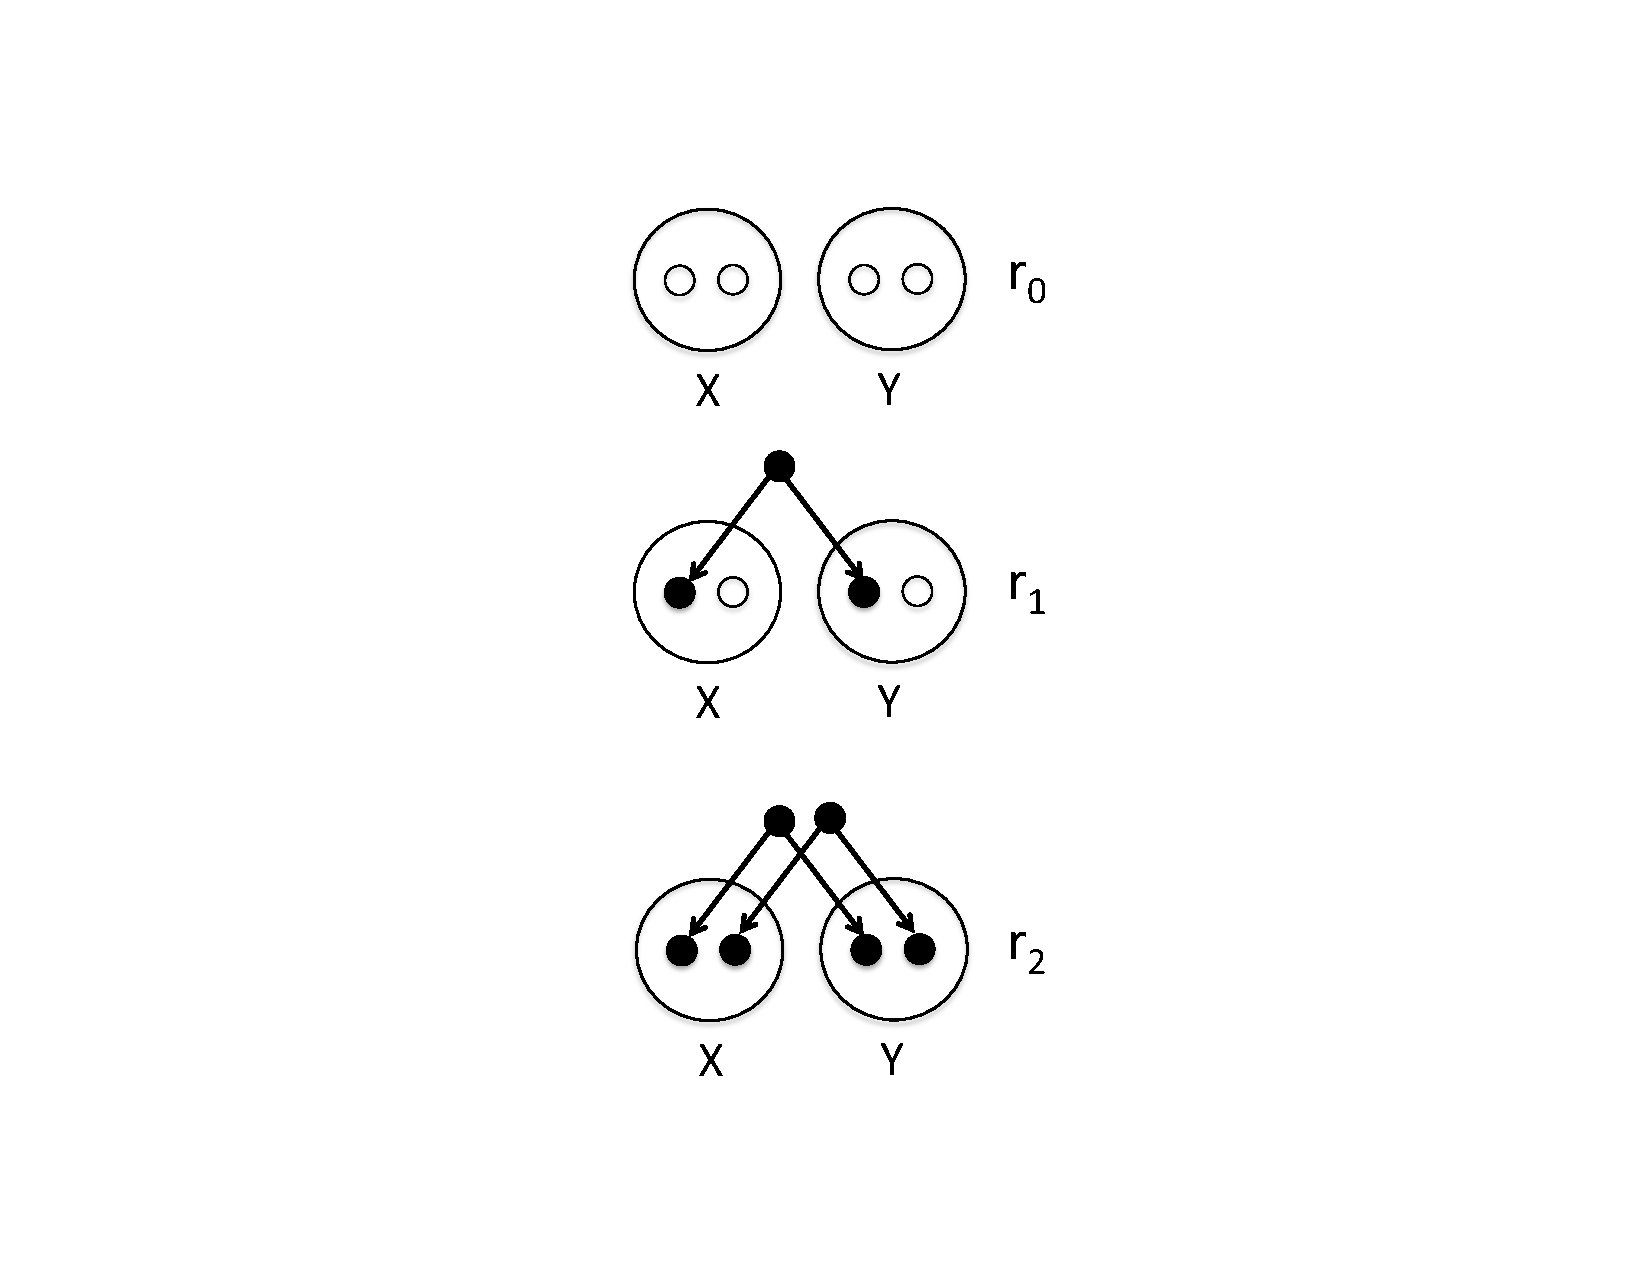
\includegraphics[width= 0.75 \textwidth]{figures/sharing_relatives/IBD_0_1_2.pdf}
\end{center}
\caption{A pair of diploid individuals (i and j) sharing 0, 1, or 2 alleles IBD
  where lines show the sharing of alleles by descent (e.g. from a
  shared ancestor). } \label{fig:IBD_0_1_2}
\end{marginfigure}

In the above step, eqn\eqref{eqn:coeffkinship_step}, we're summing the
conditional probability of alleles $I$ \& $J$ being IBD over whether our individuals $i$ \& $j$ share $0$, $1$,
or $2$ alleles IBD, an example of using the Law of Total Probability (see Appendix
eqn \eqref{eqn:law_tot_prob}).  We've then, in eqn \ref{eqn:coeffkinship}, used the fact that we can
calculate our condition probabilities of  I \& J being IBD using the
rules of Mendelian transmision. Consider the probability $
P(\text{I\&J IBD} |~ \text{i\&j  1 IBD})$, i.e. that our
pair of alleles ($I$ \& $J$) drawn from individuals $i$ and $j$ are IBD given that
$i$ and $j$ share one allele IBD, this is a $\nicefrac{1}{4}$ as we need to
draw the allele that is IBD from both $i$ and $j$, i.e. drawing both black
alleles in the middle panel of Figure \ref{fig:IBD_0_1_2}, which
happens with probability $\nicefrac{1}{2} \times \nicefrac{1}{2} $. 
The coefficient of kinship will appear multiple times, in both our discussion of
inbreeding and in the context of phenotypic resemblance between relatives.\\

\begin{table*}
\begin{center}
\begin{tabular}{ l c c c c}
\hline
Relationship (i,j)$^{*}$ & $P(\text{i\&j  0 IBD}) $ & $P(\text{i\&j  1 IBD}) $ & $P(\text{i\&j  2 IBD}) $ & $P(\text{I\&J IBD} )$\\
  \hline
  Relationship (i,j)$^{*}$ & $r_0$ & $r_1$ & $r_2$ & $F_{ij}$\\
    \hline
parent--child & 0 & 1 & 0 & \nicefrac{1}{4}\\
full siblings & \nicefrac{1}{4} & \nicefrac{1}{2} & \nicefrac{1}{4} & \nicefrac{1}{4}\\
Monozygotic twins  & 0 & 0 & 1  & \nicefrac{1}{2} \\
$1^{st}$ cousins & \nicefrac{3}{4} & \nicefrac{1}{4} & 0 & \nicefrac{1}{16}\\
\hline
\end{tabular}
\end{center}
\caption{Probability that two individuals of a given relationship share 0, 1, or 2 alleles
identical by descent on the autosomes. $^{*}$Assuming that our
individuals are outbred and that this the only close relationship the pair shares. } % doesn't this implicitly assume an infinite population?
\label{table:IBDprobs}
\end{table*}

\begin{question}
  What are $r_0$, $r_1$, and $r_2$ for $\nicefrac{1}{2}$ sibs? ($\nicefrac{1}{2}$ sibs share one
parent but not the other).
\end{question}

\begin{question}
  Explain in words why $ P(\text{I\&J IBD} |~ \text{i\&j  2 IBD}) = \nicefrac{1}{2}$.
\end{question}

%Question 5. Consider a biallelic locus where allele 1 is at fre- quency p, and two individuals who have IBD allele sharing probabili- ties r0, r1, r2.
%What is the overall probability that these two individuals are both homozygous for allele 1?

\paragraph{Genotypic sharing between pairs of individuals.}
Our $r$ coefficients are going to have various uses. For example, they allow us
to calculate the probability of the genotypes of a pair of
relatives. Consider a biallelic locus where allele $A_1$ is
at frequency $p$, and two individuals who have IBD allele sharing
probabilities $r_0$, $r_1$, $r_2$. What is the overall probability that these
two individuals are both homozygous for allele 1? Well that's
\begin{align}
  P(A_1 A_1) = & P(A_1 A_1 | \text{0 alleles IBD}) P(\text{0 alleles IBD})  \nonumber\\
  & + P(A_1 A_1 | \text{1 allele IBD}) P(\text{1 allele IBD})  \nonumber\\
  &+ P(A_1 A_1 | \text{2 alleles IBD}) P(\text{2 alleles IBD})
\end{align}
Or, in our $r_0$, $r_1$, $r_2$ notation:
\begin{align}
  P(A_1 A_1) = & P(A_1 A_1 | \text{0 alleles IBD}) r_0  \nonumber\\
  & + P(A_1 A_1 |
  \text{1 alleles IBD}) r_1  \nonumber\\
  & + P(A_1 A_1 | \text{2 alleles IBD}) r_2 \label{eqn:initial_relly_IBD_calc}
\end{align}
If our pair of relatives share $0$ alleles IBD, then the probability that
they are both homozygous is $P(A_1 A_1 |
\text{0 alleles IBD}) =p^2 \times p^2$, as all four alleles
represent independent draws from the population. If they share $1$
allele IBD, then the shared allele is of type $A_1$ with probability $p$, and then
the other non-IBD allele, in both relatives, also needs
to be $A_1$ which happens with probability $p^2$, so $P(A_1 A_1 |
\text{1 alleles IBD})=p \times p^2$. Finally, our pair of relatives can
share two alleles IBD, in which case $P(A_1 A_1 | \text{2 alleles IBD})
= p^2$, because if one of our individuals is homozygous for the $A_1$ allele,
both individuals will be. Putting this all together our equation
\eqref{eqn:initial_relly_IBD_calc} becomes
\begin{equation}
P(A_1 A_1) = p^4 r_0 + p^3 r_1 + p^2 r_2 \label{eqn:IBD_relly_calc}
\end{equation}
Note that for specific cases we could also calculate this by summing over all the
possible genotypes their shared ancestor(s) had; however, that would be much more
involved and not as general as the form we have derived here.

We can write out terms like eq \eqref{eqn:IBD_relly_calc} for all of
the possible configurations of genotype
sharing/non-sharing between a pair of individuals. Based on this we can write down the expected number of
polymorphic sites where our individuals are observed to share 0, 1, or 2
alleles.

\begin{question} [Trickier question.]
The genotype of our suspect in Question \ref{Q:CODIS} turns out to be 100/80 for
D16S539 and 70/80 at TH01. The suspect is not a match to the DNA
from the crime scene; however, they could be a sibling.

Calculate the joint probability of observing the genotype from the crime and our
suspect:\\
{\bf A)} Assuming that they share no close relationship.\\
%JRI: pretty sure the answer key is wrong here. If we put your eact set of fractions into R we get 1.433992e-09 as the answer. So something is wrong somewhere in answer.

{\bf B)} Assuming that they are full sibs.\\

{\bf C)} Briefly explain your findings.
  \end{question}

 \begin{marginfigure}
\begin{center}
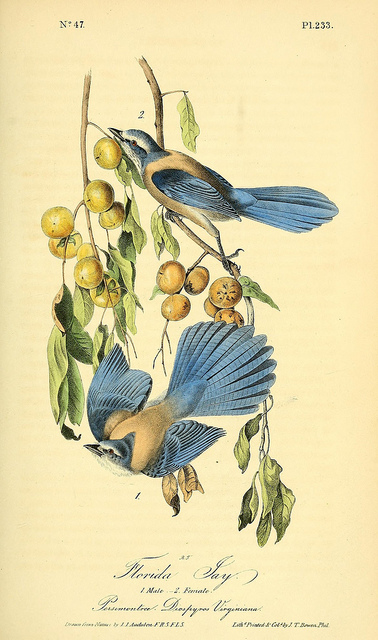
\includegraphics[width= \textwidth]{illustration_images/alleles_genotypes/Florida_scrub_jay/8576533889_3a131ffc4c_z.jpg}
\end{center}
\caption{Florida Scrub-Jays ({\it Aphelocoma coerulescens}). \BHLCC{The birds of America : from drawings made in the United
    States and their territories. 1880. Audubon
    J.J.}{https://www.biodiversitylibrary.org/page/40447048\#page/169/mode/1up}{Smithsonian
    Libraries}{2.0} } \label{fig:FSJ}
\end{marginfigure}


There's a variety of ways to estimate the relationships among
individuals using genetic data.  An example of using allele sharing to identify relatives is offered by
the work of Nancy Chen \citep[in collaboration with Stepfanie
Aguillon, see ][]{chen:16,Aguillon:17}. \citeauthor{chen:16} has collected genotyping data from thousands of
Florida Scrub Jays at over ten thousand loci. These Jays live at the
Archbold field site, and have been carefully monitored for many
decades allowing the pedigree of many of the birds to be known.
Using these data she estimates allele frequencies at each
locus. Then by equating the observed number of times that a pair of
individuals share $0$, $1$, or $2$ alleles to the theoretical
expectation, she estimates the probability of $r_0$, $r_1$, and
$r_2$ for each pair of birds. A plot of these are shown in Figure
\ref{fig:FSJ_IBD}, showing how well the estimates match those known
from the pedigree.
%\end{question}


\begin{figure}
\begin{center}
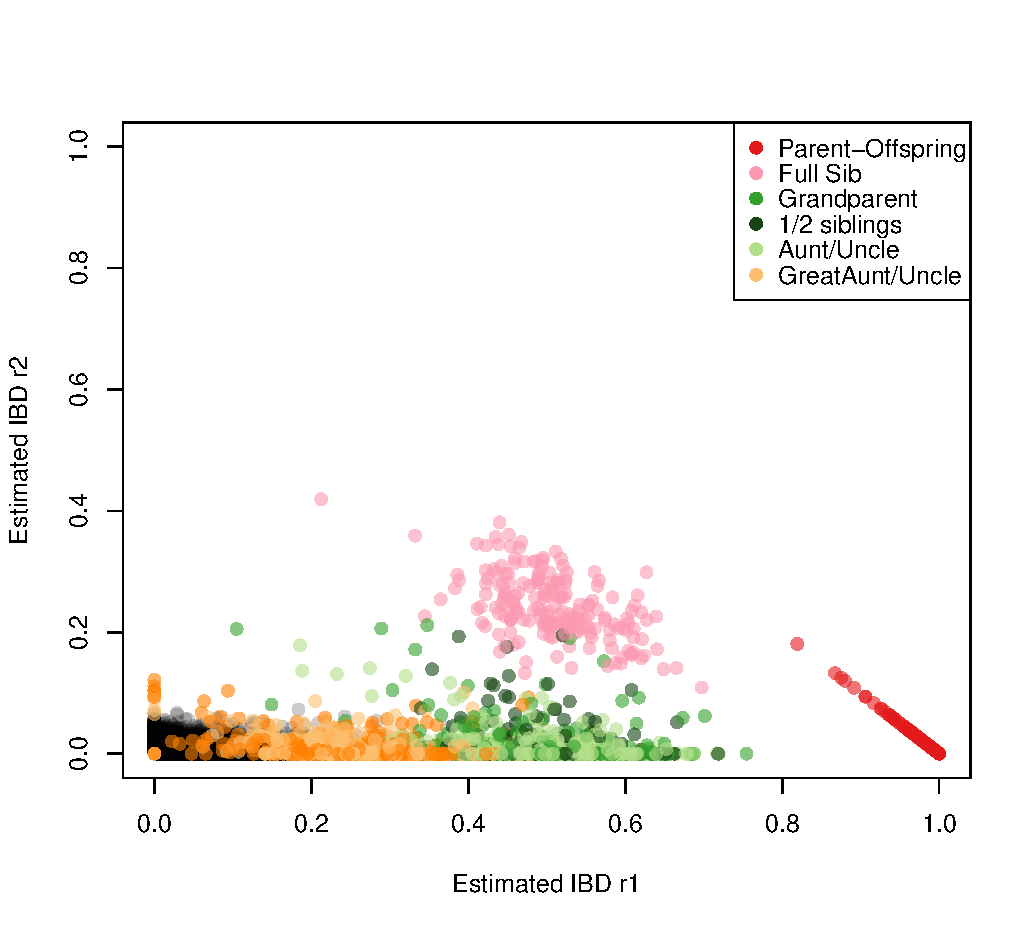
\includegraphics[width= 0.75 \textwidth]{figures/FSJ_IBD.pdf}
\end{center}
\caption[3cm]{Estimated coefficient
of kinship from Florida Scrub Jays. Each point is a pair of
individuals, plotted by their estimated IBD ($r_1$ and $r_2$) from their genetic data. The
points are coloured by their known pedigree relationships. Note that
most pairs have low kinship, and no recent genealogical relationship,
and so appear as black points in the lower left corner. Thanks to
Nancy Chen for supplying the data. \gitcode{https://github.com/cooplab/popgen-notes/blob/master/Rcode/FSJ_IBD/FSJ_IBD_plotting.R} } \label{fig:FSJ_IBD}
\end{figure}

\paragraph{Sharing of genomic blocks among relatives.}
\begin{figure}
\begin{center}
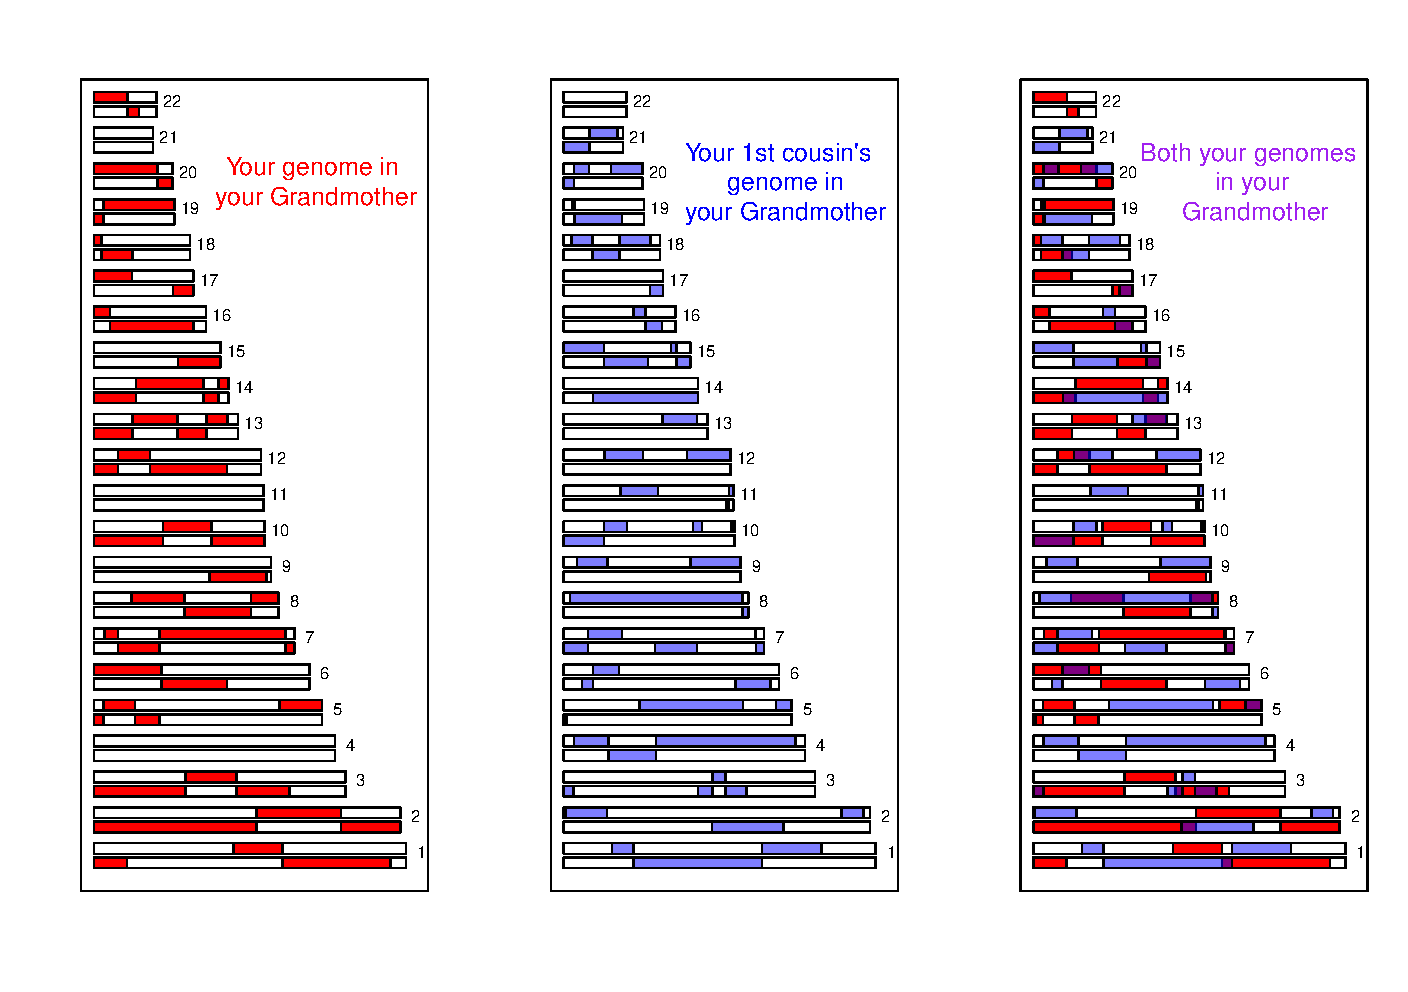
\includegraphics[width= \textwidth]{figures/sharing_relatives/First_cousin_overlap.pdf}
\end{center}
\caption[]{A simulation of sharing between first cousins. The regions of your grandmother's 22 autosomes that you inherited are
coloured red, those that your cousins inherited are coloured blue. In the third panel we show the overlapping genomic regions in purple, these regions will be IBD in you and your cousin. If you are full first cousins, you will also have shared genomic regions from your shared grandfather, not shown here. Details about how we made these simulations \href{https://gcbias.org/2013/12/02/how-many-genomic-blocks-do-you-share-with-a-cousin/}{here}.
} \label{fig:first_cousin_IBD}
\end{figure}
We can more directly see the sharing of the genome among close
relatives using high-density SNP genotyping arrays. In Figure \ref{fig:first_cousin_IBD} we show a simulation of you and your first cousin's genomic material that you both inherited from your shared grandmother. Colored purple are regions where you and your cousin will have matching genomic material, due to having inherited it IBD from your shared grandmother.
%JRI: text says ``Below'' but float ends up above



You and your first cousin will share at least one allele of your genotype at all of the polymorphic loci in these purple regions. There's a range of methods to detect such sharing. One way is to look for unusually long stretches of the genome where two individuals are never homozygous for different alleles. By identifying pairs of individuals who share an unusually large number of such putative IBD blocks, we can hope to identify unknown relatives in genotyping datasets. In fact, companies like 23\&me and Ancestry.com use signals of IBD to help identify family ties.

As another example, consider the case of third cousins. You share one of eight sets of great-great grandparents with each of your (likely many) third cousins. On average, you and each of your third cousins each inherit one-sixteenth of your genome from each of those two great-great grandparents. This turns out to imply that on average, a little less than one percent of your and your third cousin's genomes ($2 \times (1/16)^2 =0.78\%$) will be identical by virtue of descent from those shared ancestors. A simulated example where third cousins share blocks of their genome (on chromosome 16 and 2) due to their great, great grandmother is shown in Figure \ref{fig:third_cousin_IBD}.

\begin{figure}
\begin{center}
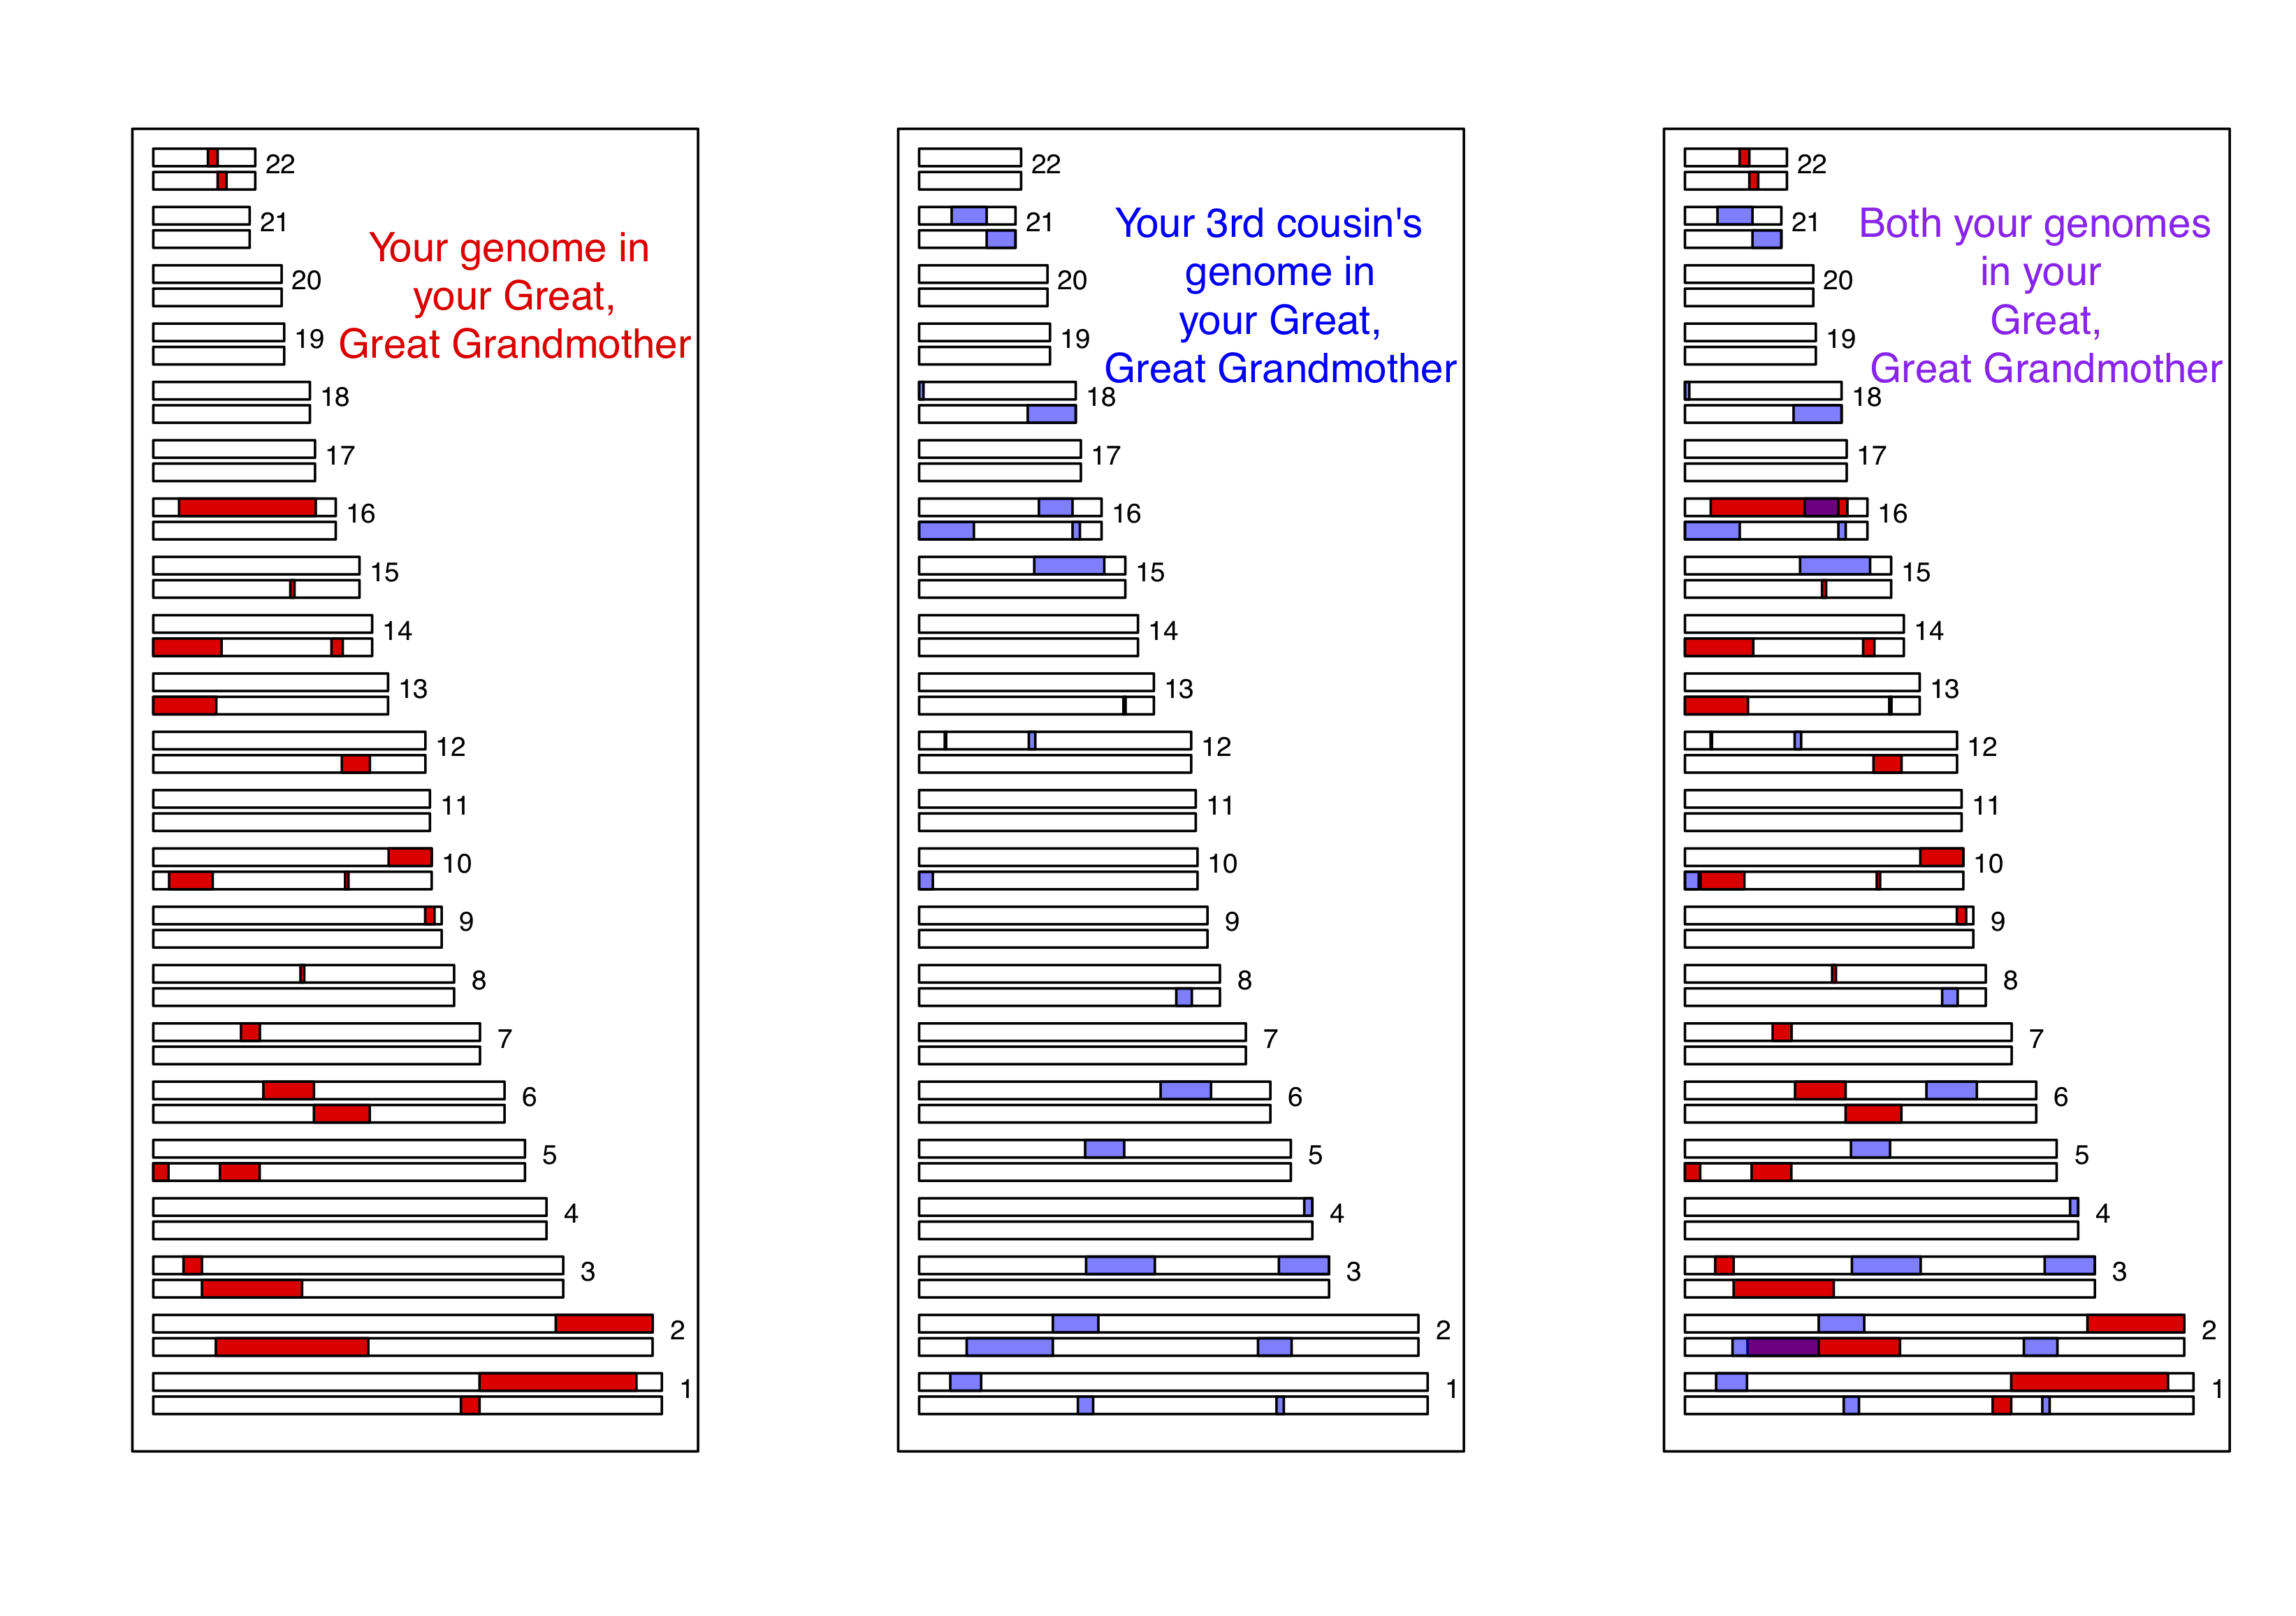
\includegraphics[width= \textwidth]{figures/sharing_relatives/Third_cousin_overlap_1.png}
\end{center}
\caption[]{A simulation of sharing between third cousins, the details are the same as in Figure \ref{fig:first_cousin_IBD}.} \label{fig:third_cousin_IBD}
\end{figure}


Note how if you compare Figure \ref{fig:third_cousin_IBD} and Figure \ref{fig:first_cousin_IBD}, individuals inherit less IBD from a shared great, great grandmother than from a shared grandmother, as they inherit from more total ancestors further back. Also notice how the sharing occurs in shorter genomic blocks, as it has passed through more generations of recombination during meiosis. These blocks are still detectable, and so third cousins can be detected using high-density genotyping chips, allowing more distant relatives to be identified than single marker methods alone. \sidenote{Indeed the suspect in case of the Golden State Killer was identified through identifying third cousins that genetically matched a DNA sample from an old crime scene (see a \href{https://gcbias.org/2018/05/07/how-lucky-was-the-genetic-investigation-in-the-golden-state-killer-case/}{here} for more details).} More distant relations than third cousins, e.g. fourth cousins, start to have a significant probability of sharing none of their genome IBD. But you have many fourth cousins, so you will share some of your genome IBD with some of them; however, it gets increasingly hard to identify the degree of relatedness from genetic data the deeper in the family tree this sharing goes.

\subsection{Inbreeding}
We can define an inbred individual as an individual whose parents are
more closely related to each other than two random individuals drawn
from some reference population.  \\


\begin{marginfigure}
\begin{center}
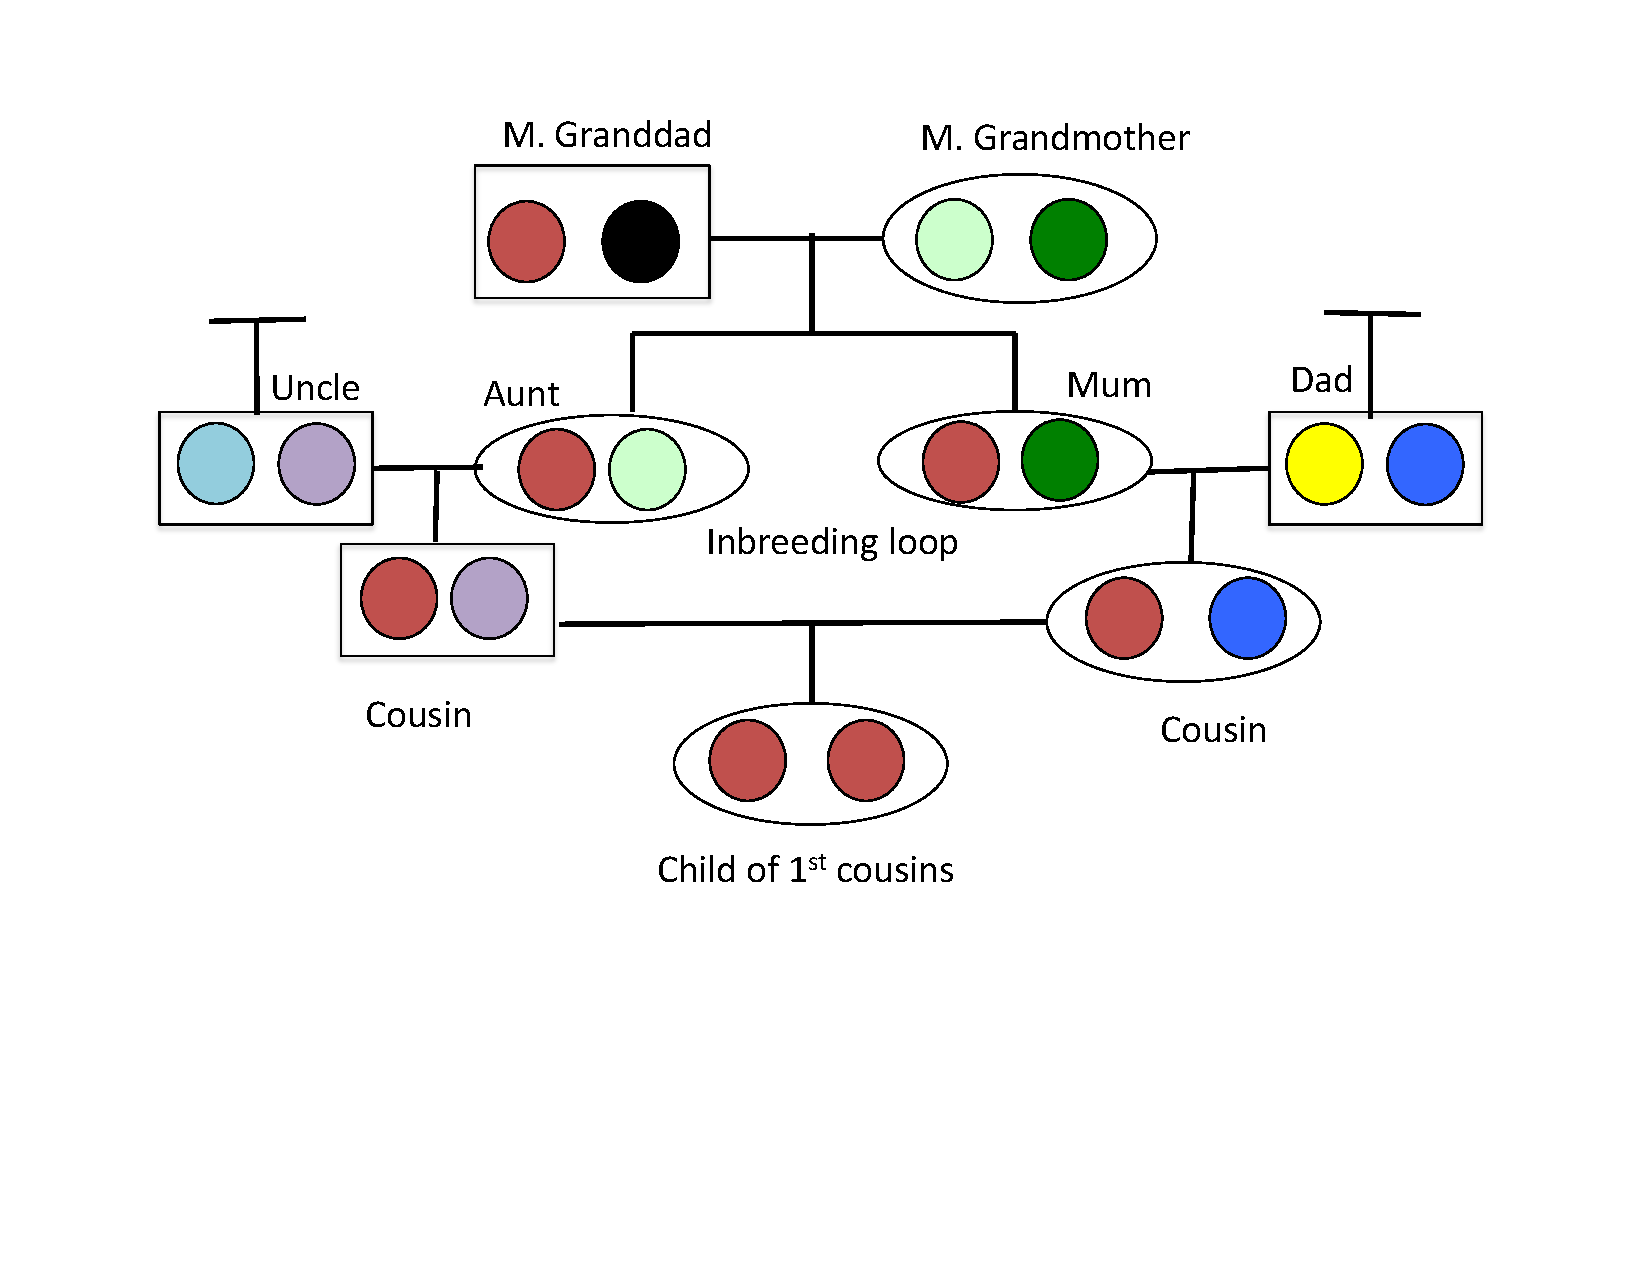
\includegraphics[width= \textwidth]{figures/Child_first_cousins_Homozy_BD.pdf}
\end{center}
\caption{Alleles being transmitted through an inbred pedigree. The two sisters (mum and aunt) share two alleles identical by descent (IBD). The cousins share one
  allele IBD. The offspring of first cousins is homozygous by
  descent at this locus.} \label{fig:IBD_cousins_cartoon}
\end{marginfigure}
\graham{Change this to have squares and circles}
When two related individuals produce an offspring, that individual can
receive two alleles that are identical by descent, i.e.\ they
can be homozygous by descent (sometimes termed autozygous), due to the
fact that they have two copies of an allele through different paths
through the pedigree.  This increased likelihood of being homozygous
relative to an outbred individual is the most obvious effect of
inbreeding. It is also the one that will be of most interest to us, as it
underlies a lot of our ideas about inbreeding depression and
population structure. For example, in Figure \ref{fig:IBD_cousins_cartoon} our
offspring of first cousins is homozygous by descent having received
the same IBD allele via two different routes around an inbreeding loop.\\

As the offspring receives a random allele from each parent ($i$ and $j$), the
probability that those two alleles are identical by descent is equal to the
kinship coefficient $F_{ij}$ of the two parents (Eqn.\ \ref{eqn:coeffkinship}). This follows from the fact that
the genotype of the offspring is made by sampling an allele at random from each
of our parents. % We will use IBD for identical by descent. \\ %% this was already defined above.

\begin{table}
\begin{center}
\begin{tabular}{ccc}
\hline
$f_{11}$ & $f_{12}$ & $f_{22}$ \\
\hline
$(1-F) p^2 + F p$ & $(1-F) 2pq$ & $(1-F) q^2 + F q$ \\
\hline
\end{tabular}
\end{center}
\caption{\textbf{Generalized Hardy--Weinberg}} \label{table:GeneralizedHWE}
\end{table}

The only way the offspring can be heterozygous ($A_1 A_2$) is if their two
alleles at a locus are not IBD (otherwise they would necessarily be
homozygous). Therefore, the probability that they are heterozygous is

\begin{equation}
(1-F) 2p q,
\label{eq:hetGenHW}
\end{equation}
%
where we have dropped the indices $i$ and $j$ for simplicity.  The offspring
can be homozygous for the $A_1$ allele in two different ways.  They can have
two non-IBD alleles that are not IBD but happen to be of the allelic type
$A_1$, or their two alleles can be IBD, such that they inherited allele $A_1$
by two different routes from the same ancestor. Thus, the probability that an
offspring is homozygous for $A_1$ is

\begin{equation}
(1-F) p^2 + F p.
\end{equation}
%
Therefore, the frequencies of the three possible genotypes can be written as given in
Table \ref{table:GeneralizedHWE}, which provides a generalization of the Hardy--Weinberg
proportions.\\


%Note that the generalized Hardy--Weinberg proportions completely
%specify the genotype probabilities, as there are two parameters ($p$ and $F$)
%and two degrees of freedom (as $p$ and $q$ have to sum to one).
%Therefore, any combination of genotype frequencies at a biallelic site
%can be specified by a combination of $p$ and $F$.\\
%JRI: unclear to me if this is useful. will readers understand parameter numbers/DF?

\begin{question}
The frequency of the $A_1$ allele is $p$ at a biallelic locus. Assume that our population is randomly mating and that the
genotype frequencies in the population follow from HW. We select two
individuals at random to mate from this population. We then mate the children
from this cross. What is the probability that the child from this full
sib-mating is
homozygous?
\end{question}

\paragraph{Multiple inbreeding loops in a pedigree.}
Up to this point we have assumed that there is at most one inbreeding loop in the recent family history of our
  individuals, i.e. the parents of our inbred individual have at most one recent genealogical connection. However, an individual who has multiple inbreeding loops in their pedigree can be homozygous by
  descent thanks to receiving IBD alleles via multiple different different loops. To calculate inbreeding in pedigrees of arbitrary complexity, we can extend
 beyond our original relatedness coefficients $r_0$, $r_1$, and $r_2$ to account for
 higher order sharing of alleles IBD among relatives. For example,
 we can ask, what is the probability that \textit{both} of the alleles in the first individual
 are shared IBD with one allele in the second individual? There are
 nine possible relatedness coefficients in total to completely describe kinship between two diploid individuals, and we won't go in to them here
 as it's a lot to keep track of.
However, we will show how we can calculate the inbreeding coefficient of an
individual with multiple inbreeding loops more directly.\\

%ut at loci where the ancestor is inbred you get two more options (C inherits maternal/B paternal or opp.) so the factor of 2 applies to fA as well and cancels out for both.}

Let's say the parents of our inbred individual (B and C) have $K$ shared ancestors,
i.e. individuals who appear in both B and C's recent family trees. We denote these shared ancestors by $A_1, \dots,A_K$, and we denote by $n$ the total number of individuals in the chain from B to C via ancestor $A_i$, including B, C, and $A_i$. For example, if B is C's aunt, then B and C share two ancestors, which are B's parents and, equivalently, C's grandparents. In this case, there are n=4 individuals from B to C through each of these two shared ancestor. In the general case, the kinship coefficient of B and C,
i.e. the inbreeding coefficient of their child, is
\begin{equation}
 F = \sum_{i=1}^K \frac{1}{2^{n_i}} \big( 1+ f_{A_i} \big)
\end{equation}
where $f_{A_i}$ is the inbreeding coefficient of the ancestor
$A_i$. What's happening here is that we sum over all the mutually-exclusive paths in the pedigree through which B and C can share an allele IBD. With probability
$\nicefrac{1}{2^{n_i}}$, a pair of alleles picked at random from B and C is descended from the same ancestral allele in individual
$A_i$, in which case the alleles are IBD. \sidenote{For example, in the case of our aunt-nephew case, assuming that the aunt's two parents are their only recent shared ancestors, then $F = \nicefrac{1}{2^4}+\nicefrac{1}{2^4} = \nicefrac{1}{8}$, in agreement with the answer we would obtain from  eqn \eqref{eqn:coeffkinship}.} However, even if B inherits the maternal allele and C inherits the paternal allele of shared ancestor $A_i$, if $A_i$ was
themselves inbred,  with probability $f_{A_i}$ those two
alleles are themselves IBD. Thus a shared \textit{inbred} ancestor further increases
the kinship of B and C.

\begin{figure}
  \begin{center}
  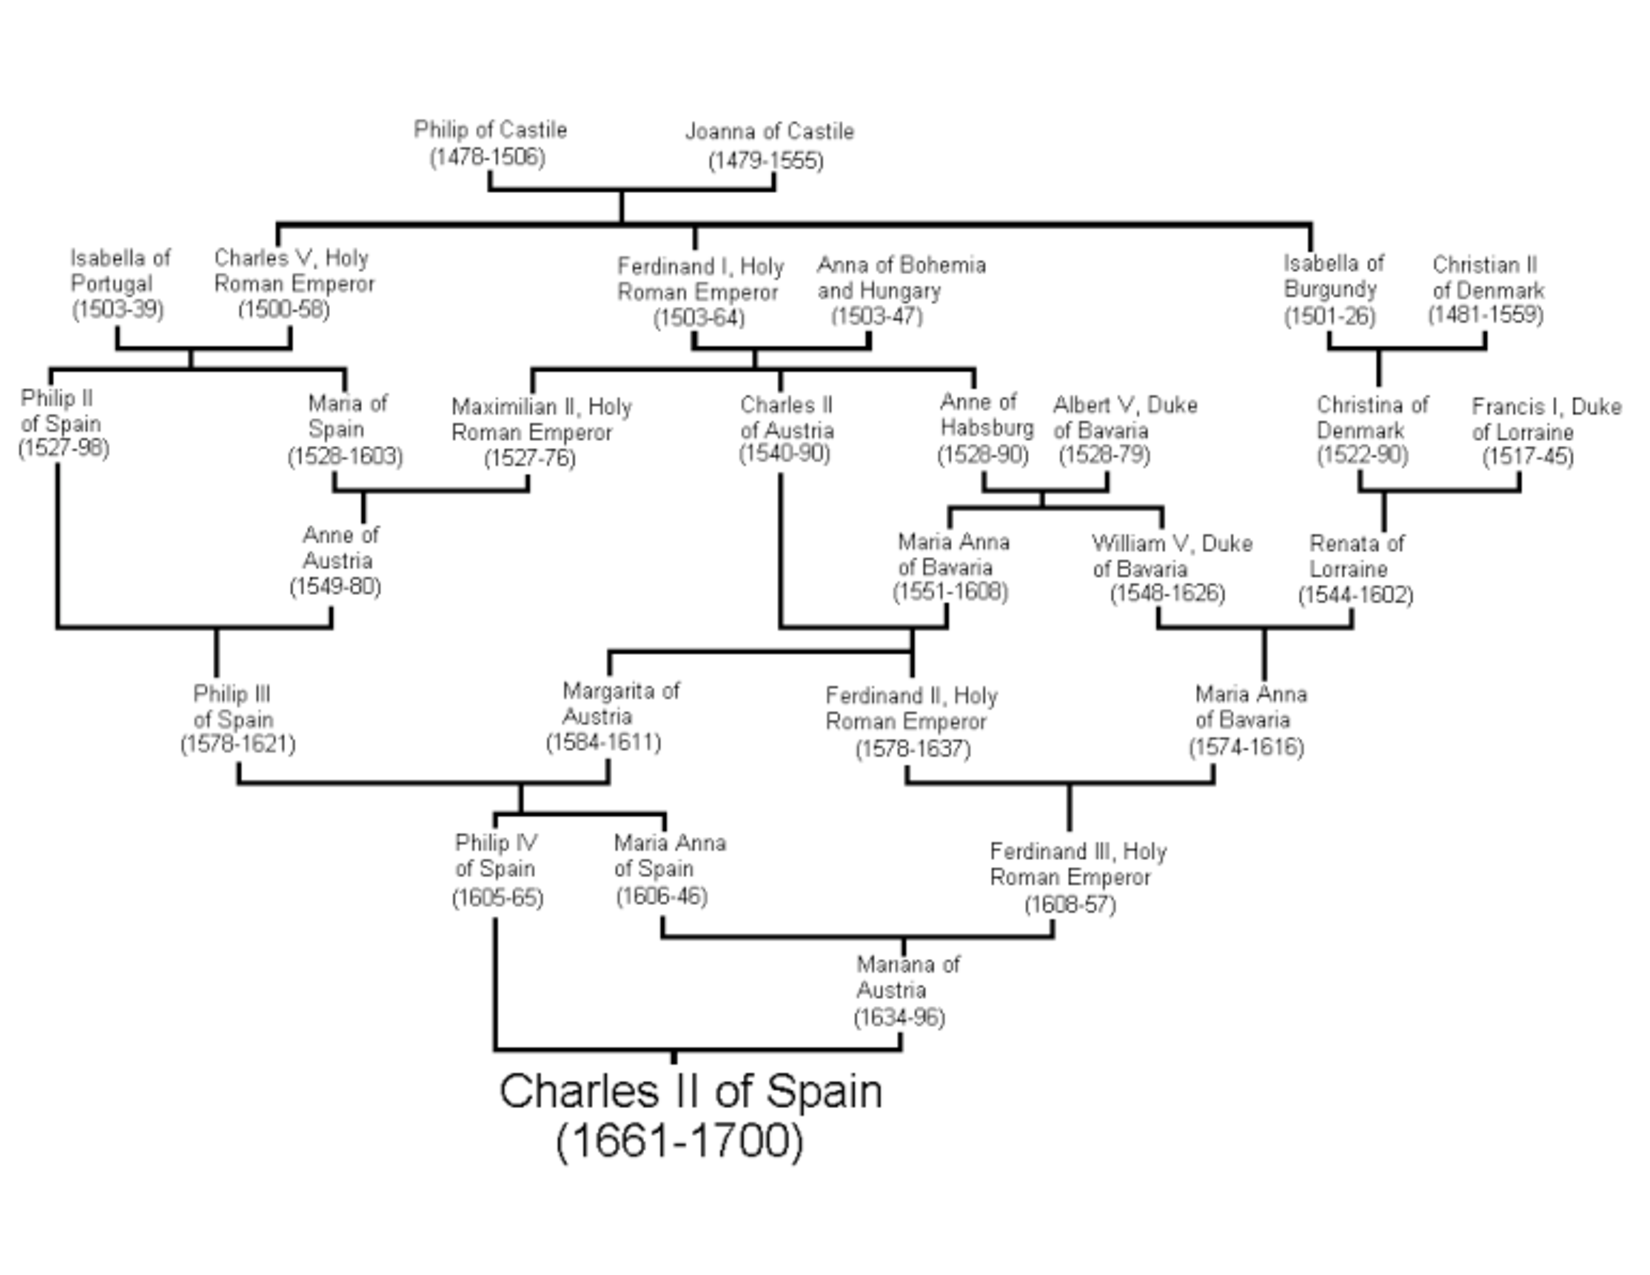
\includegraphics[width=
  \textwidth]{Journal_figs/alleles_genotypes/Charles_second_pedigree/Carlos_second_pedigree_2_trimmed.pdf}  %https://commons.wikimedia.org/wiki/File:Carlos_segundo80.png
\end{center}
\caption{The pedigree of King Charles II of
  Spain. Pedigree from
  \href{https://commons.wikimedia.org/wiki/File:Carlos_segundo80.png}{wikimedia}
drawn by \href{https://en.wikipedia.org/wiki/User:Lec_CRP1}{Lec CRP1},
public domain.} \label{fig:Carlos_second_pedigree}
\end{figure}
\begin{marginfigure}
\begin{center}
  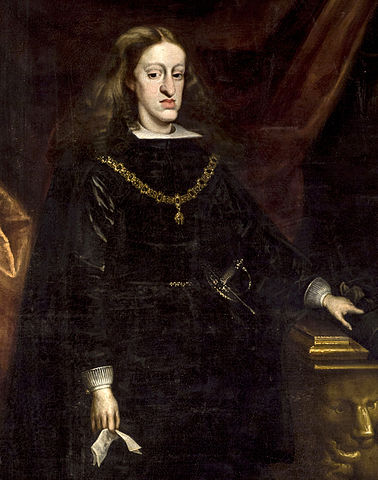
\includegraphics[width=
  \textwidth]{illustration_images/alleles_genotypes/Carlos_second/378px-Juan_de_Miranda_Carreno_002.jpg}
%https://commons.wikimedia.org/wiki/File:Carlos_segundo80.png
\end{center}
\caption{Charles II of Spain (by Juan Carre\~{n}o de Miranda,
  1685). \href{https://it.wikipedia.org/wiki/Carlo_II_di_Spagna\#/media/File:Juan_de_Miranda_Carreno_002.jpg}{Public Domain}.} \label{fig:Carlos_second}
\end{marginfigure}
Multiple inbreeding loops increase the probability that a child
is homozygous by descent at a locus, which can be calculated simply by plugging in $F$, the child's
inbreeding coefficient, into our generalized HW equation.


As one extreme example of the impact of multiple inbreeding loops in
an individual's pedigree, let's consider king Charles II of
Spain, the last of the Spanish Habsburgs.  Charles was the son of
Philip IV of Spain and Mariana of Austria, who were uncle and
niece. If this were the only inbreeding loop, then Charles would have had an
inbreeding coefficient of $\nicefrac{1}{8}$. Unfortunately for Charles, the
Spanish Habsburgs had long kept wealth and power within their family
by arranging marriages between close kin. The pedigree of Charles II is shown in Figure \ref{fig:Carlos_second_pedigree}, and
multiple inbreeding loops are apparent. For example, Phillip III,
Charles II's grandfather and great-grandfather, was himself a child of
an uncle-niece marriage.

\citet{alvarez:09} calculated that Charles II had an inbreeding
coefficient of $0.254$, equivalent to a full-sib mating,
thanks to all of the inbreeding loops in his pedigree. Therefore, he
is expected to have been homozygous by descent for a full quarter of his
genome. As we'll talk about later in these notes, this means that Charles
may have been homozygous for a number of recessive disease alleles,
and indeed he was a very sickly man who left no descendants due to his
infertility. \sidenote{Pedro Gargantilla, who performed Charles's autopsy, stated
  that his body ``did not contain a single drop of blood; his heart was
  the size of a peppercorn; his lungs corroded; his intestines rotten
  and gangrenous; he had a single testicle, black as coal, and his
  head was full of water.'' While some of this description
  may refer to actual medical conditions, some of these details seem a
  little unlikely. See
  \href{https://www.thevintagenews.com/2017/03/23/when-charles-ii-of-spain-died-the-autopsy-stated-that-his-body-did-not-contain-a-single-drop-of-blood-and-his-head-was-full-of-water/}{here}.
} Thus plausibly the end of one of the great
European dynasties came about through inbreeding. 
%JRI: good idea to include links to potentially impermanent websites?


\subsection{Calculating inbreeding coefficients from genetic data}

%JRI: you transition from an individual's inbreeding coefficient here to using F as a population inbreeding parameter. i think some text explaining this change of scope might help

If the observed heterozygosity in a population is $H_O$, and we assume that the
generalized Hardy--Weinberg proportions hold, we can set $H_O$ equal to
$f_{12}$, and solve Eq.\ \eqref{eq:hetGenHW} for $F$ to obtain an estimate of
the inbreeding coefficient as

\begin{equation}
\hat{F} = 1-\frac{f_{12}}{2pq} = \frac{2pq - f_{12}}{2pq}.
\label{eqn:Fhat}
\end{equation}

As before, $p$ is the frequency of allele $A_{1}$ in the population. This can
be rewritten in terms of the observed heterozygosity ($H_O$) and the
heterozygosity expected in the absence of inbreeding, $H_E=2pq$, as
\begin{equation}
\hat{F} = \frac{H_E-H_O}{H_E} = 1 - \frac{H_O}{H_E}.
\label{eqn:FhatHO}
\end{equation}
Hence, $\hat{F}$ quantifies the deviation due to inbreeding of the observed heterozygosity from the one expected under random mating, relative to the latter.

\begin{question}
  Suppose the following genotype frequencies were observed for an esterase locus in a population of \textit{Drosophila} (A denotes the ``fast" allele and B denotes the ``slow" allele):
\begin{center}
\begin{tabular}{ccc}
\hline
AA &	AB &	BB\\
\hline
0.6 &	0.2 &	0.2\\
\end{tabular}
\end{center}
What is the estimate of the inbreeding coefficient at the esterase locus?
\end{question}

If we have multiple loci, we can replace $H_O$ and $H_E$ by their means
over loci, $\bar{H}_O$ and $\bar{H}_E$, respectively. Note that, in principle, we could also calculate $F$ for each individual locus first, and then take the average across loci. However, this procedure is more prone to introducing a bias if sample sizes vary across loci, which is not unlikely when we are dealing with real data.


Genetic markers are commonly used to estimate inbreeding for wild and/or captive populations of conservation concern. As an example of this, consider the case of the Mexican wolf ({\it Canis lupus baileyi}), a sub-species of gray wolf. \begin{marginfigure}[-2cm]
\begin{center}
  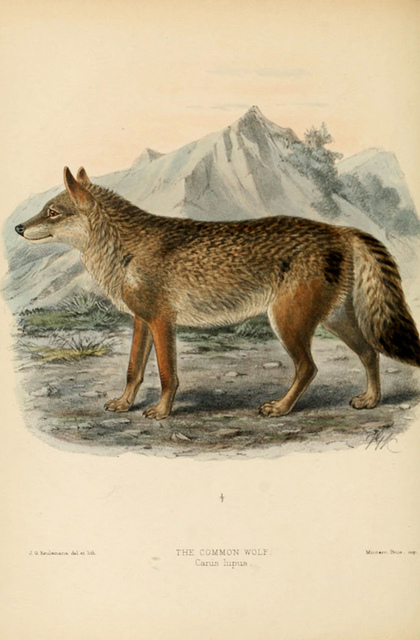
\includegraphics[width= \textwidth]{illustration_images/alleles_genotypes/grey_wolf/5988399184_0c36a8e51c_z.jpg}
\end{center}
\caption{Grey wolf ({\it Canis lupus}). \BHLNC{Dogs, jackals, wolves,
    and foxes: a monograph of the Canidae. 1890. y J.G. Keulemans}{https://www.biodiversitylibrary.org/page/17002968\#page/58/mode/1up}{University of Toronto - Gerstein Science Information Centre}} \label{fig:Grey_wolf}
\end{marginfigure}
They were extirpated in the wild during the mid-1900s due to hunting, and the remaining five Mexican wolves in the wild were captured to start a breeding program. \citet{vonHoldt:11} estimated the current-day, average expected heterozygosity to be $0.18$, based on allele frequencies at over forty thousand SNPs. However, the average Mexican wolf individual was only observed to be heterozygous at $12\%$ of these SNPs. Therefore, the average inbreeding coefficient for the Mexican wolf is $F = 1 -\nicefrac{0.12}{0.18}$, i.e. $\sim 33 \%$ of a lobo's genome is homozygous due to recent inbreeding in their pedigree.

%{\bf Q}\arabic{Question} \refstepcounter{Question}

%==Phenotypic resemblance between relatives ==
%<source-file filename="Quantative_traits.tex" display="Quantative_traits.wrapped.latexml.xhtml">

%==Phenotypic resemblance between relatives ==
%<source-file filename="Quantative_traits.tex" display="Quantative_traits.wrapped.latexml.xhtml">

  \paragraph{Genomic blocks of homozygosity due to inbreeding.}

As we saw above, close relatives are expected to share alleles IBD in
large genomic blocks. Thus, when related individuals mate and transmit
alleles to an inbred offspring, they transmit these alleles in big
blocks through meiosis. An example, lets return to the case of our
hypothetical first cousins from Figure
\ref{fig:IBD_cousins_chr_cartoon}. If this pair of individuals had a
child, one possible pattern of genetic transmission is shown in Figure
\ref{fig:kid_first_cousins}. The child has inherited the red stretch
of chromosome via two different routes through their predigree from
the grandparents. This is an example of an autozygous
segment, where the child is homozygous by descent at all of the loci in this
red region.
  \begin{figure}
  \begin{center}
    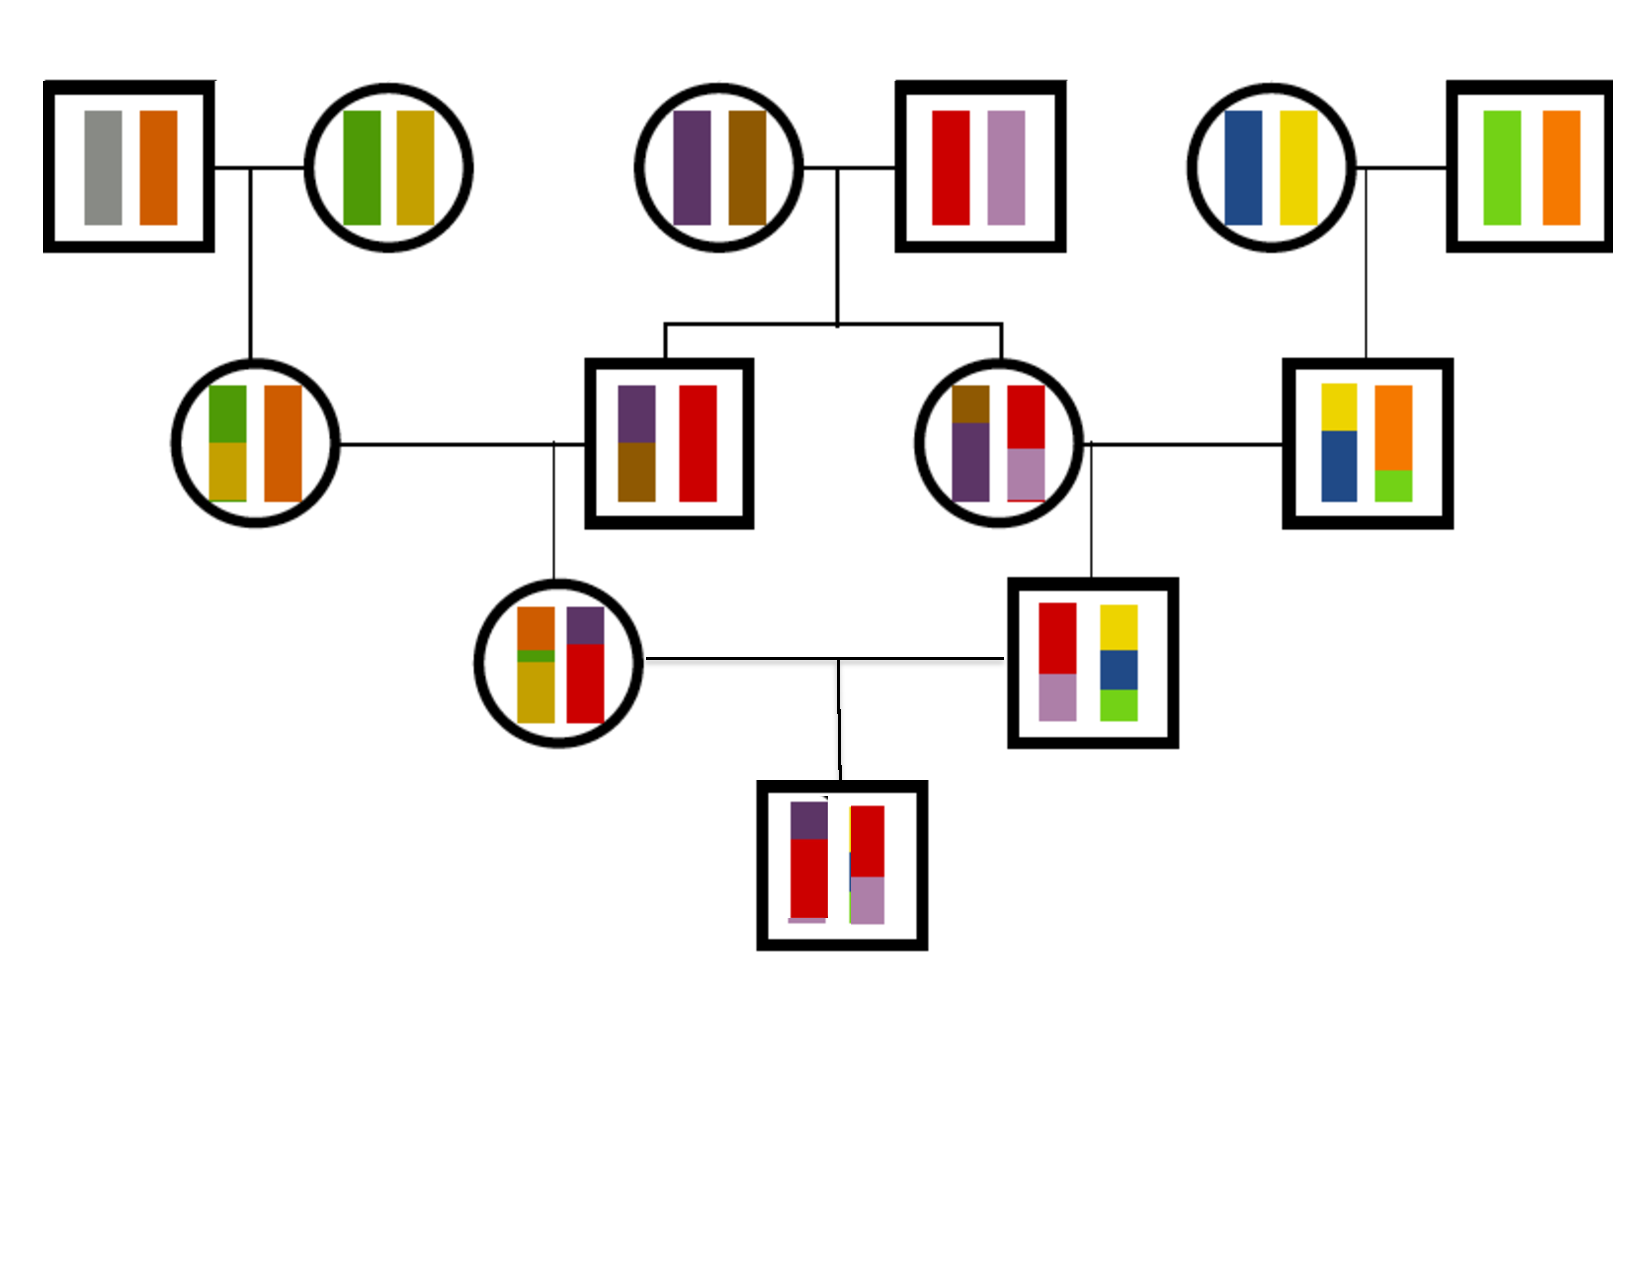
\includegraphics[width= 0.75 \textwidth]{figures/sharing_relatives/first_cousin_offspring.pdf}
\end{center}
\caption{A pedigree showing the offspring of first cousins. The
  chromosomes of their great-grandparents are coloured different colours
so their transmission can be tracked. The child is homozygous by
descent (HBD) for a section of the red chromosome.} \label{fig:kid_first_cousins}
\end{figure}
The inbreeding coefficient of the child sets the proportion of their
genome that will be in these autozygous segments. For example, a child
of first full cousins is expected to have $1/16$ of their
genome in these segments.
The more distant the loop in the pedigree, the more meioses that
chromosomes have been through and the shorter individual blocks will be. A
child of first cousins will have longer blocks than a child of second
cousins, for example.

Individuals with multiple inbreeding loops in their family tree can
have a high inbreeding coefficient due to
the combined effect of many small blocks of autozygosity. For example, Charles II had
an inbreeding coefficient that is equivalent to that of the child of
full-sibs, with a quarter of his genome expected to homozygous by
descent, but this would be made up of many shorter blocks.
%With multiple rounds of inbreeding individuals can

We can hope to detect these blocks by looking for unusually long
genomic runs of homozygosity (ROH) sites in an individual's genome. One way to
estimate an individual's inbreeding coefficient is then to total up
the proportion of an individual's genome that falls in such ROH
regions. This estimate is called $F_{ROH}$.

\graham{update to use figs from G3 Sam's article, and collapse to
  single ref.}
An example of using $F_{ROH}$ to study inbreeding comes from the work of
\citet{sams2018fine}, who identified runs of homozygosity in 2,500 dogs,
ranging from 500kb up to many megabases.
  \begin{figure}
  \begin{center}
    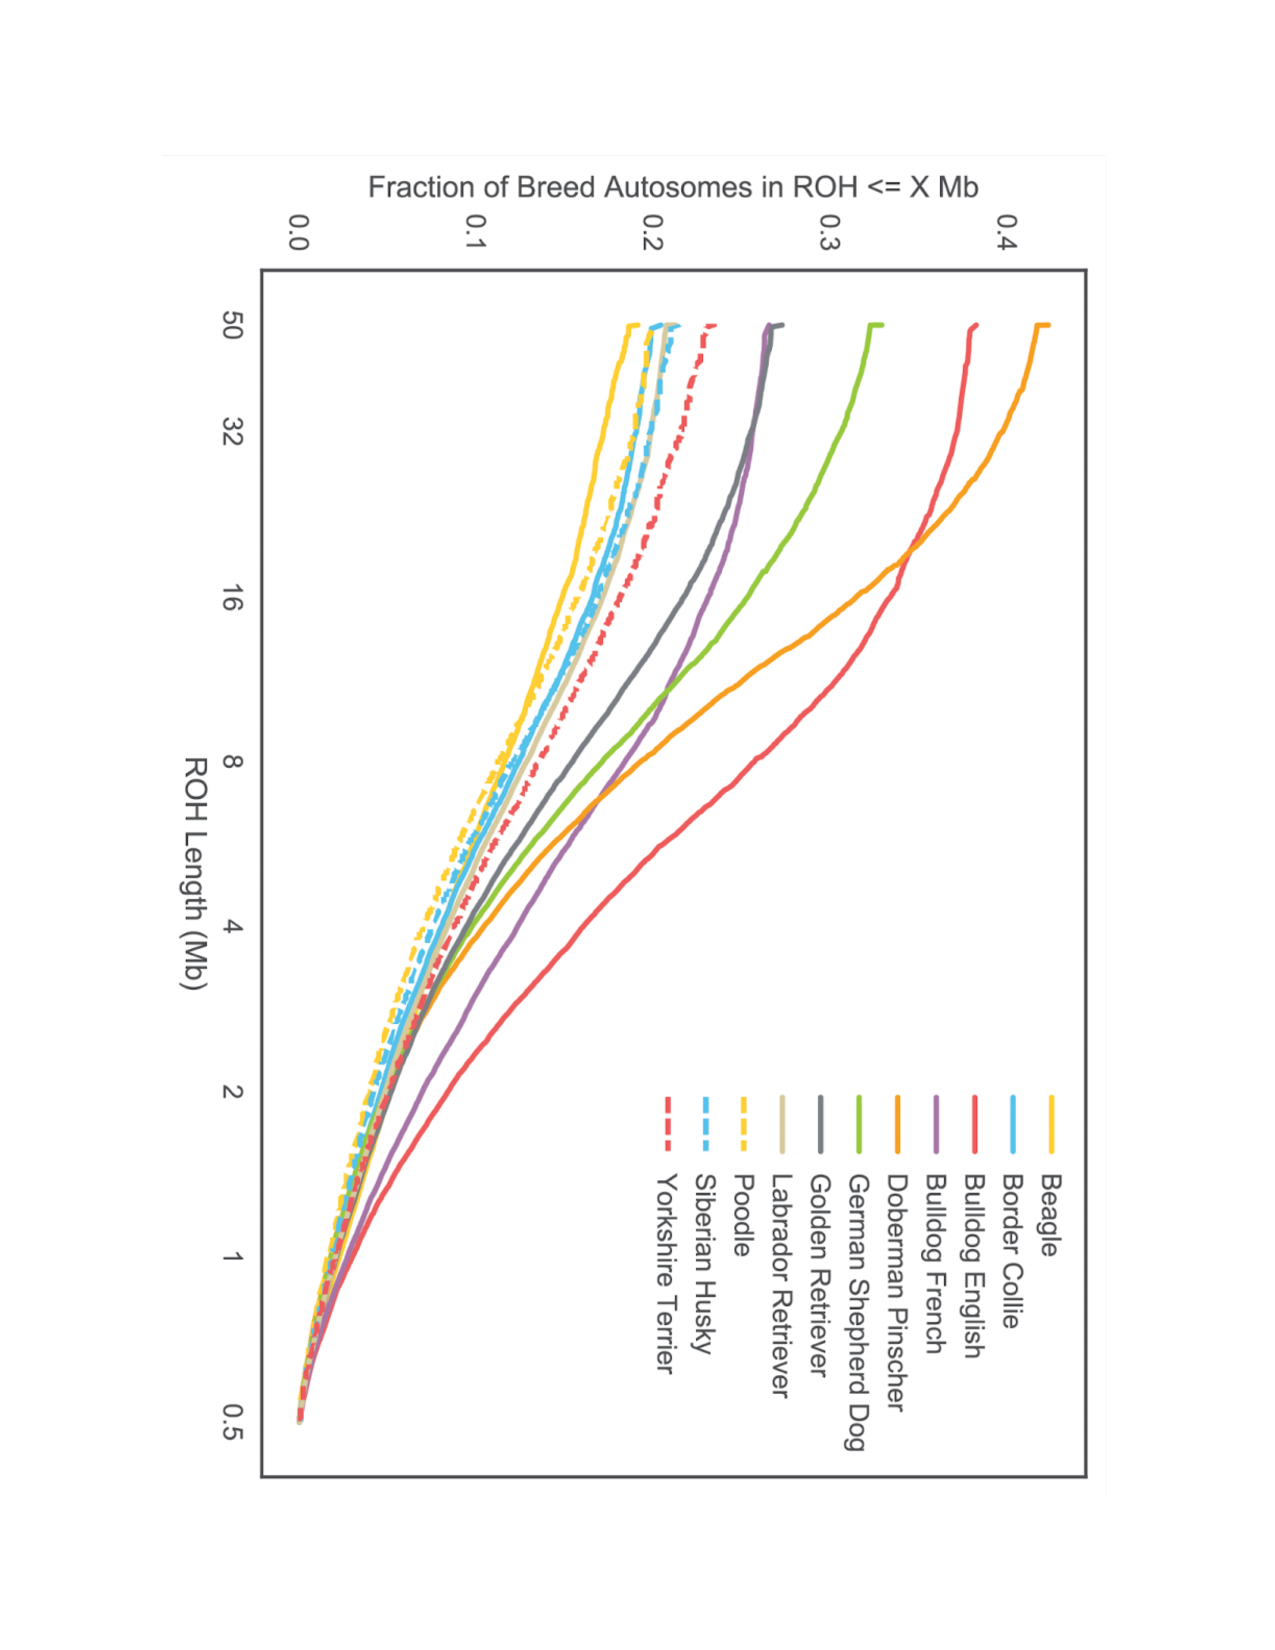
\includegraphics[width= \textwidth]{figures/sharing_relatives/dogs_FROH.pdf}
\end{center}
\caption{The distribution  of $F_{ROH}$ of individuals from various
  dog breeds from \citet{Sams:18}, \PLOSccBY.} \label{fig:dog_FOH}
\end{figure}
Figure
\ref{fig:dog_FOH} shows the distribution of $F_{ROH}$ of individuals in each dog
breed for the X and autosome. In Figure \ref{fig:dog_FOH_dist} this is
broken down by the length of ROH segments.
%JRI: No text reference to this figure. Why show a bulldog and not a mix of dog breeds?

  \begin{marginfigure}[-1cm]
  \begin{center}
    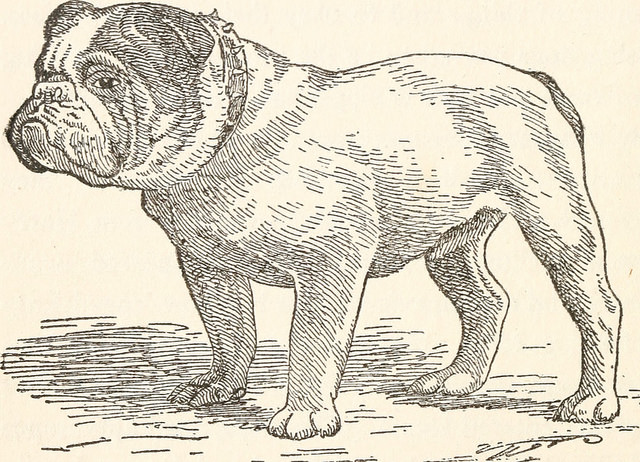
\includegraphics[width=
    \textwidth]{illustration_images/alleles_genotypes/english_bulldog/14752595581_4330377c97_z.jpg}
\end{center}
\caption{English bulldog. The dogs of Boytown. 1918.  Dyer, W. A.} \label{fig:bulldog}
\end{marginfigure}

Dog breeds have been subject
to intense breeding that has resulted in high levels of inbreeding. Of the population samples examined, Doberman Pinschers have the highest levels of their genome in runs of
homozygosity ($F_{ROH}$), somewhat higher than English bulldogs. In \ref{fig:dog_FOH_dist} we can see that English bulldogs have more short ROH than Doberman Pinschers, but that Doberman Pinschers have more of their genome in very large ROH ($>16 Mb$). This suggests that English bulldogs have had long history of inbreeding but that Doberman Pinschers have a lot of recent inbreeding in their history.

  \begin{figure}
  \begin{center}
    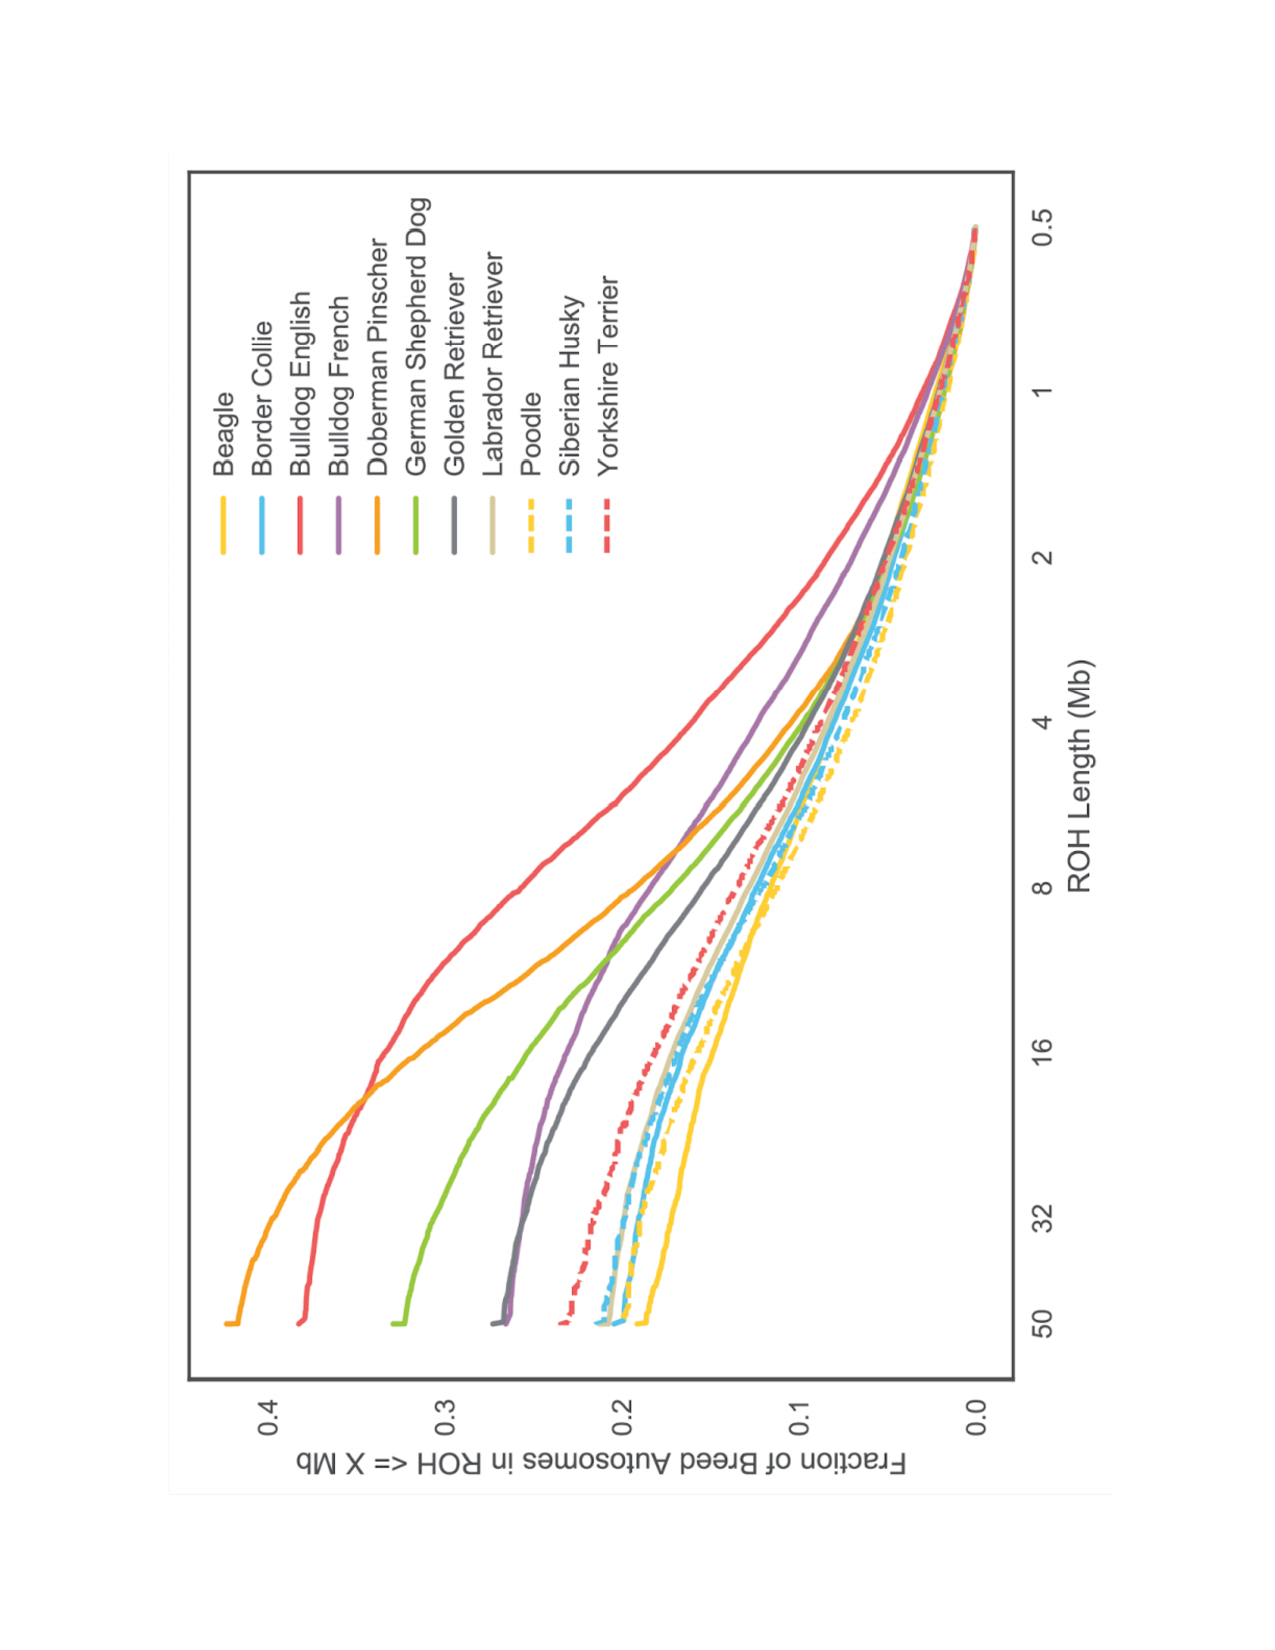
\includegraphics[width= \textwidth]{figures/sharing_relatives/dog_FROH_dist.pdf}
\end{center}
\caption{Cumulative density of ROH length, measured in megabases (Mb) from \citet{Sams:18} for various
  dog breeds (\PLOSccBY). Note that longer lengths of ROH are on the left of the plot.} \label{fig:dog_FOH_dist}
\end{figure}

\section{Genetic Drift and Neutral Diversity}

Various sources of randomness are inherent in evolution.  One major source of
stochasticity in population genetics is genetic drift.  Genetic drift occurs
because more or less copies of an allele by chance can be transmitted to the
next generation. This can occur because by chance the individuals carrying a
particular allele can leave more or less offspring in the next generation. In a
sexual population genetic drift also occurs because Mendelian transmission
means that only one of the two alleles in an individual, chosen at random at a
locus, is transmitted to the offspring. 

Genetic drift can play a role in the dynamics of all alleles and populations,
but it will play the biggest role for neutral alleles. A neutral polymorphism
occurs when the segregating alleles at a polymorphic site have no discernible
differences in their effect on fitness. We'll make clear what we mean by discernible later, for
the moment think of this as ``no effect" on fitness. 


\subsection{Loss of heterozygosity due to drift.} \label{LossofHet} 

Genetic drift will, in the absence of new mutations, slowly purge our
population of neutral genetic diversity as alleles slowly drift to high or low
frequencies and are lost or fixed over time. \\

Imagine a population of a constant size $N$ diploid individuals, and that we
are examining a locus segregating for two alleles that are neutral with respect
to each other.  This population is randomly mating with respect to the alleles
at this locus. See Figures \ref{fig:LossHet_two_alleles} and
\ref{fig:LossHet_many_alleles} to see how genetic drift proceeds, by tracking
alleles within a small population. \\

In generation $t$ our current level of heterozygosity is $H_t$,
i.e. the probability that two randomly sampled alleles in generation
$t$ are non-identical is $H_t$. Assuming that the mutation rate is
zero (or vanishing small), what is our level of heterozygosity in
generation $t+1$?\\

\begin{figure}
\begin{center}
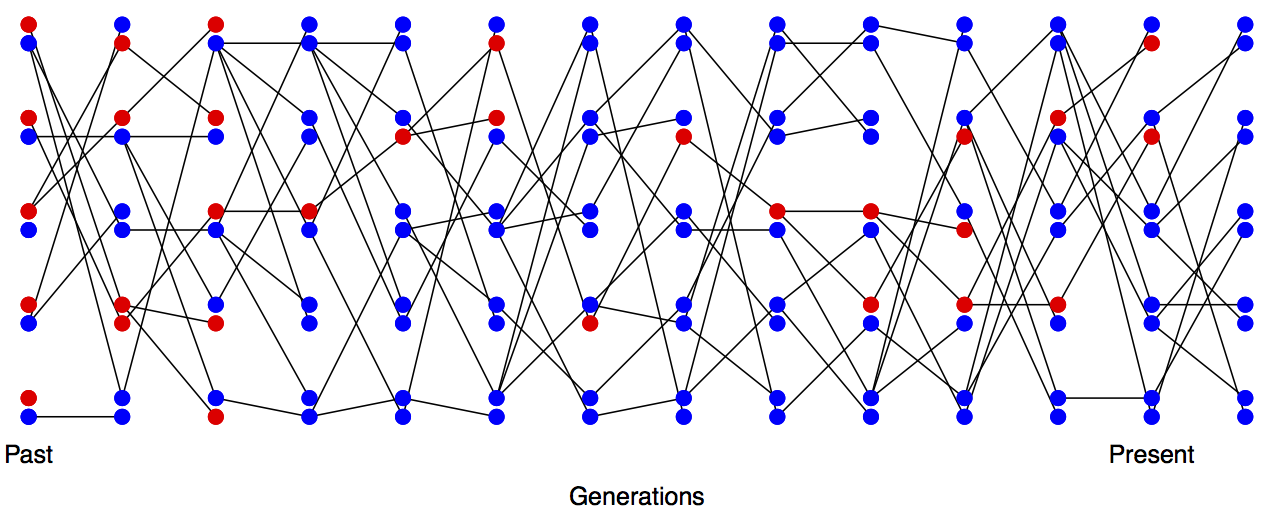
\includegraphics[width= \textwidth]{figures/Loss_of_he_col_two_alleles.png}
\end{center}
\caption{Loss of heterozygosity over time, in the absence of new
  mutations. A diploid population of 5 individuals over the
  generations, with lines showing transmission. In the first
  generation every individual is a heterozygote.} \label{fig:LossHet_two_alleles}
\end{figure} 

\begin{figure}
\begin{center}
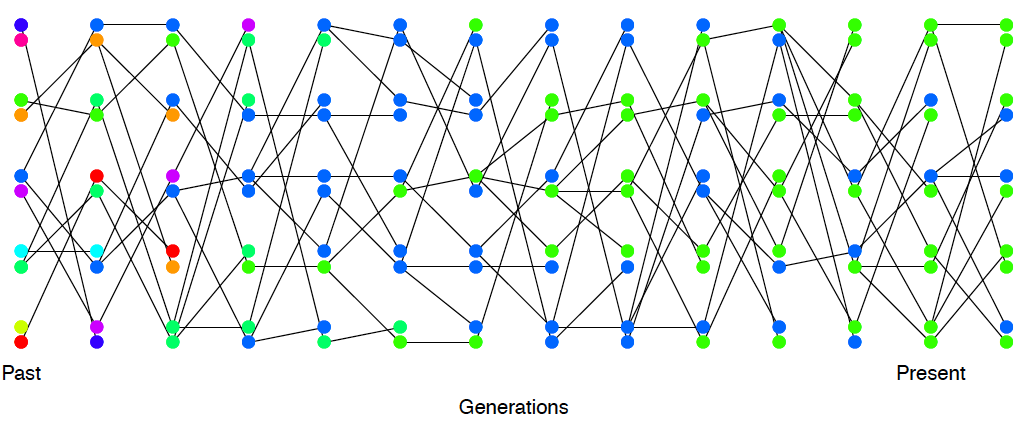
\includegraphics[width= \textwidth]{figures/Loss_of_het_2_many_alleles.png}
\end{center}
\caption{Loss of heterozygosity over time, in the absence of new
  mutations. A diploid population of 5 individuals. In the first generation I colour every allele a different
colour so we can track their descendants.} \label{fig:LossHet_many_alleles}
\end{figure} 

In the next generation ($t+1$) we are looking at the alleles in the
offspring of generation $t$. If we randomly sample two alleles in generation
$t+1$ which had different parental alleles in generation $t$ then it
is just like drawing two random alleles from generation $t$. So the
probability that these two alleles in generation $t+1$, that have
different parental alleles in generation $t$, are non-identical is
$H_t$. \\

Conversely, if our pair of alleles have the same parental allele in
the proceeding generation (i.e. the alleles are identical by descent
one generation back) then these two alleles must be identical (as we
are not allowing for any mutation). \\

In a diploid population of size $N$ individuals there are $2N$ alleles. The
probability that our two alleles have the same parental allele in the
proceeding generation is $\nicefrac{1}{(2N)}$, the probability that they have
different parental alleles is is $1-\nicefrac{1}{(2N)}$. So by the above
argument the expected heterozygosity in generation $t+1$ is
%
\begin{equation}
H_{t+1} = \frac{1}{2N} \times 0 + \left(1-\frac{1}{2N} \right)H_t
\end{equation}
%
By this argument if the heterozygosity in generation $0$ is $H_0$ our
expected heterozygosity in generation $t$ is
%
\begin{equation}
H_t = \left(1-\frac{1}{2N} \right)^tH_0
\end{equation}
%
i.e. the expected heterozygosity with our population is decaying
geometrically with each passing generation. If we assume that $\nicefrac{1}{(2N)}
\ll 1$ then we can approximate this geometric decay by an exponential
decay (see Question \ref{geo_question} below), such that
%
\begin{equation}
H_t =H_0 \exp \left(-\frac{t}{2N} \right)  
\end{equation}
%
i.e. heterozygosity decays exponentially at a rate
$\nicefrac{1}{(2N)}$.

Note how this picture of decreasing heterozygosity is in contrast to the
consistency of Hardy--Weinberg equilibrium of the previous chapter. 
However, our Hardy-Weinberg \emph{proportions} hold in forming each new
generation. As the offspring genotypes in the next generation ($t+1$) represent a random
draw from the previous generation ($t$). If the parental frequency is $p_t$ we
\emph{expect} a proportion $2p_t(1-p_t)$ of our offspring to be
heterozygotes (and HW proportions for our homozygotes). However, because of population size is finite the
observed genotype frequencies in the offspring will (likely) not match exactly with our
expectations. As our genotype frequencies likely change slightly due
to sampling, biologically this reflects random variation in family size
and Mendelian segregation, the allele frequency will changed. 
Therefore, while each generation represents a sample from
Hardy-Weinberg proportions based on the generation before, our
genotype proportions is not a equilbrium (an unchanging state) as the
underyling allele frequency changes over the generations. We'll develop some mathematical models for these allele
frequency changes later on. For now we'll simply note that
under our simple model of drift (formally the Wright Fisher model) our
allele count in the $t+1^{th}$ generation represents a binomial sample
(of size $2N$) from the popuation frequency $p_t$ in the previous
generation.  

% generation $t$ may differ
%from that of $t+1$. We'll develop some mathematical models for these allele
%frequency changes 
 %from the previous generation we are
%drawing alleles at random from the  
%Here, the
%freqeuncy of each genotype will likely change, due to chance fluctuations in
%the underlying allele frequency $p$. While within a single generation
%Hardy--Weinberg proportions are maintained (at least approximately), across
%generations the genotypic frequencies change with allele frequency. The change
%in allele frequencies is due to drift: due to random variation in family size
%and Mendelian segregation, the allele frequency in generation $t$ may differ
%from that of $t+1$. We'll develop some mathematical models for these allele
%frequency changes later on.

\begin{question} You are in charge of maintaining a population of delta smelt
  in the Sacramento river delta. Using a large set of microsatellites you
  estimate that the mean level of heterozygosity in this population is 0.005.
  You set yourself a goal of maintaining a level of heterozygosity of at least
  0.0049 for the next two hundred years. Assuming that the smelt have a
  generation time of 3 years, and that only genetic drift affects these loci.
  What is the smallest fully outbreeding population that you would need to
maintain to meet this goal?  (Note that while these numbers are made up, this
is similar to the calculations being carried out by conservation biologists).
\end{question}

\begin{question} \label{geo_question} In mathematical population genetics, a
  commonly used approximation $(1-x) \approx e^{-x}$ for $x << 1$ (formally
  this follows from the Taylor series expansion of $\exp(-x)$ ignoring second
  order terms of $x$).  This is especially useful for approximating a geometric
  decay process by an exponential decay process, e.g. $(1 - x)^t \approx
  e^{-xt}$. Using R, check how good of an approximation this is for three
  values of x, $x = 0.5, 0.1, 0.01$. Do this by plotting the geometric decay as
  points, and the exponential decay as a curve, using different colors for each
  of these three values. Note that you should have a discrete timescale for the
  geometric decay (e.g. using \texttt{t=seq(0, 18)}) and a near continuous scale
  for the exponential decay (e.g. using \texttt{t=seq(0, 18, length.out=100)}.
  Print off your graph and hand it in. 

    % max <- 18; x <- seq(0, max); x1 <- seq(0, max, length.out=100); plot(x, (1-0.5)^x, col='purple', pch=19); lines(x1, exp(-0.5*x1), col='purple'); points(x, (1-0.1)^x, pch=19, col='orange'); lines(x1, exp(-0.1*x1), col='orange'); points(x, (1-0.01)^x, pch=19, col='green'); lines(x1, exp(-0.01*x1), col='green') # messy but works

\end{question}

\subsection{Levels of diversity maintained by a balance between
 mutation and drift} \label{DriftMutationBalance}

Looking backwards in time from one generation to the next, we are going to say
that two alleles which have the same parental allele (i.e. find their common
ancestor) in the preceding generation have \emph{coalesced}, and refer to this
event as a \emph{coalescent event}.

The probability that our pair of randomly sampled alleles have coalesced in the
preceding generation is $\nicefrac{1}{(2N)}$, the probability that our pair of
alleles fail to coalesce is $1-\nicefrac{1}{(2N)}$. 

The probability that a mutation changes the identity of the
transmitted allele is $\mu$ per generation. So the probability of no
mutation occurring is $(1-\mu)$. We'll assume that when a mutation
occurs it creates some new allelic type which is not present in the
population. This assumption (commonly called the infinitely-many-alleles model) makes the math slightly cleaner, and also
is not too bad an assumption biologically. See Figure
\ref{fig:Mut_Sel_balance} for a depiction of mutation-drift balance in
this model over the generations.

This model let's us calculate when our two alleles last shared a common
ancestor and whether these alleles are identical as a result of
failing to mutate since this shared ancestor.  For example we can work out the probability that our
two randomly sampled alleles coalesced $2$ generations in the past
(i.e. they fail to coalesce in generation $1$ and then coalescent in
generation $2$), and
that they are identical as
\begin{equation}
\left(1- \frac{1}{2N} \right) \frac{1}{2N} (1-\mu)^4
\end{equation}
note the power of $4$ is because our two alleles have to have failed
to mutate through $2$ meioses each. 

More generally the probability that our alleles coalesce in generation
$t+1$ and are identical due to no mutation to either allele in the
subsequent generations is
%
\begin{equation}
P(\textrm{coal. in t+1 \& no mutations}) =  \frac{1}{2N} \left(1- \frac{1}{2N} \right)^t \left(1-\mu \right)^{2(t+1)}
\end{equation}
%
to make this slightly easier on ourselves let's further assume that $t
\approx t+1$ and so rewrite this as:
\begin{equation}
P(\textrm{coal. in t+1 \& no mutations}) \approx \frac{1}{2N} \left(1- \frac{1}{2N} \right)^t \left(1-\mu \right)^{2t}
\end{equation}
%

This gives us the approximate probability that two alleles will coalesce in the
$(t+1)^\text{th}$ generation. In general, we may not know when two alleles may
coalesce: they could coalesce in generation $t=1, t=2, \ldots $, and so on.
Thus, to calculate the probability that two alleles coalesce in \emph{any}
generation before mutating, we can write:

\begin{align*}
  P(\textrm{coal. in any generation \& no mutations}) &\approx P(\textrm{coal. in} \; t=1 \; \textrm{\& no mutations}) \; + \\ 
&  P(\textrm{coal. in} \; t=2 \; \textrm{\& no mutations}) + \ldots \\
  %P(\textrm{coal. in} \; t=3 \; \textrm{\& no mutations})  +\ldots \\
  &= \sum_{t=1}^\infty P(\textrm{coal. in } \; t \; \textrm{generations \& no mutation})
\end{align*}
%
which follows from the fact that coalescing in a particular generation is
mutually exclusive with coalescing in a different generation and basic probability.

While we could calculate a value for this sum given $N$ and $\mu$, it's
difficult to get a sense of what's going on with such a complicated expression.
Here, we turn to a common approximation in population genetics (and all applied
mathematics), where we assume that $\nicefrac{1}{(2N)} \ll 1$ and $\mu \ll 1$.
This allows us to approximate the geometric decay as an exponential decay.
Then, the probability two alleles coalesce in generation $t+1$ and don't mutate
can be written as:
%
\begin{align} P(\textrm{coal. in t+1 \& no mutations}) &\approx \frac{1}{2N}
\left(1- \frac{1}{2N} \right)^t \left(1-\mu \right)^{2t} \\ 
& \approx \frac{1}{2N} e^{-t/(2N)} e^{-2\mu t } \\
&=\frac{1}{2N} e^{-t(2\mu+1/(2N))} \end{align} 
%
and then we simply approximate the summation by an integral, giving us:
%
\begin{figure} \begin{center} 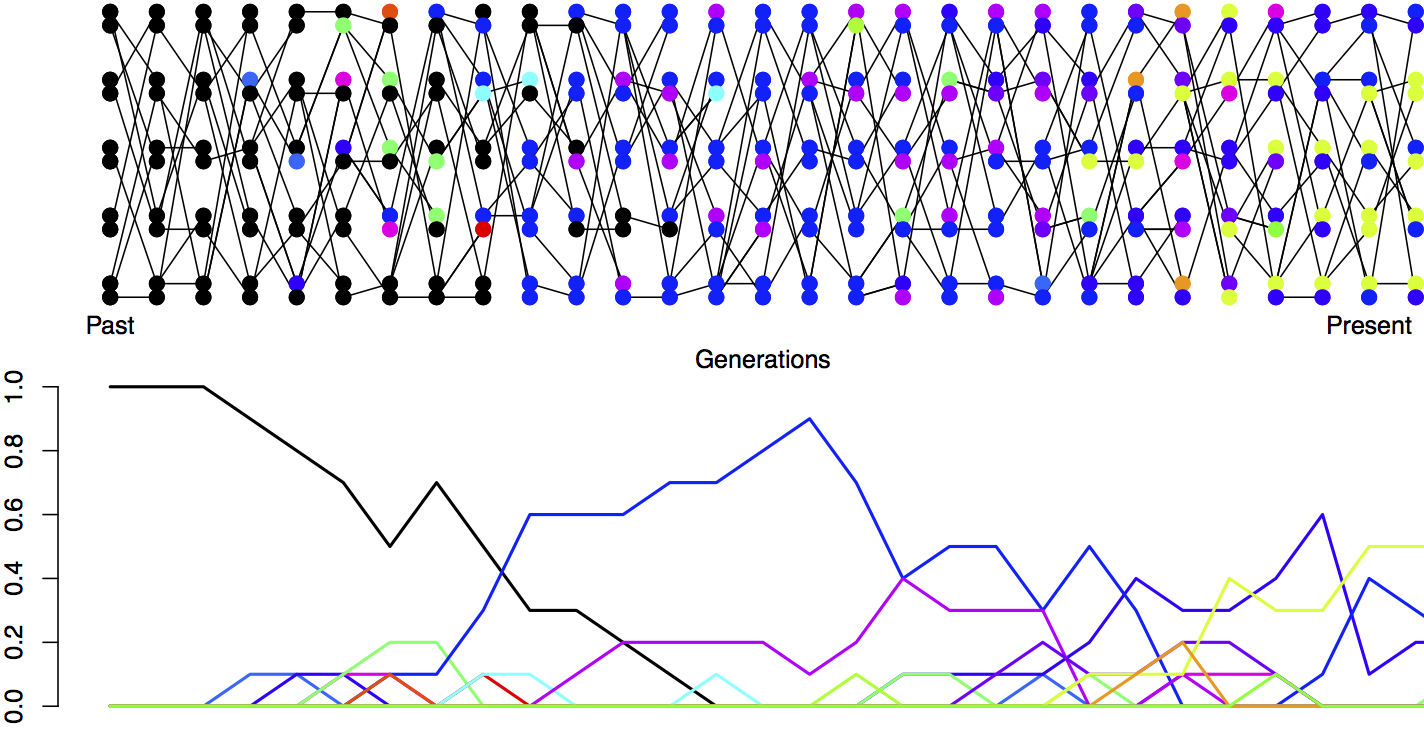
\includegraphics[width= 0.8
\textwidth]{figures/Mut_drift_balance.png} \end{center} \caption{Mutation-drift
balance. A diploid population of 5 individuals. In the first generation
everyone has the same allele (black). Each generation the transmitted allele
can mutate and we generate a new colour. In the bottom plot I trace the
frequency of alleles in our population over time.} \label{fig:Mut_Sel_balance}
\end{figure} 

\begin{equation}
\frac{1}{2N} \int_0^{\infty} e^{-t(2\mu+1/(2N))} dt =
\frac{1/(2N)}{1/(2N)+2\mu} = \frac{1}{1+4N\mu}
\end{equation}

Doing so gives us the probability that our two alleles coalesce at some point
in time, and do not mutate on either ancestral lineage to their common
ancestor. Equivalently, this can be thought about as the probability our two
alleles coalesce \emph{before} mutating. 

Then, the complementary probability that our pair of alleles are non-identical
(or heterozygous) is simply one minus this. This gives the equilibrium
heterozygosity in a population at equilibrium between mutation and drift:

\begin{equation}
  H = \frac{4N\mu}{1+4N\mu} \label{eqn:hetero}
\end{equation}
This compound parameter $4N\mu$, the population-scaled mutation rate,
will come up a number of times so we'll give it its own name
\begin{equation}
\theta = 4N\mu
\end{equation}

So all else being equal, species with larger population sizes should
have proportionally higher levels of neutral polymorphism.  If you've read to here please email Prof Coop a picture of JBS Haldane
in a striped suit with the title ``I'm reading the chapter 2 notes''. (It's well worth googling JBS Haldane and read more about his life,
he's a true character and one of the last great polymaths. )

\subsection{The effective population size}
In practice populations rarely conform to our assumptions of being
constant in size with low variance in reproduction success. Real
populations experience dramatic fluctuations in size, and there is
often high variance in reproductive success. Thus rates of drift in
natural populations are often a lot higher than the census population
size would imply.\\

To cope with this population geneticists often invoke the concept of
an effective population size ($N_e$). In many situations (but not all), departures from model assumptions can be captured by substituting $N_e$ for $N$.

Specifically the effective population size ($N_e$) is the population size that
would result in the same rate of drift in an idealized constant population size
as that observed in our true population (following our modeling assumptions).
\\

If population sizes vary rapidly in size, we can (if certain conditions are met)
replace our population size by the harmonic mean population size.
Consider a diploid population of variable size, whose size is $N_t$ $t$ generations into the
past. The probability our pairs of alleles have not coalesced by the generation $t^{th}$ is
given by
\begin{equation}
\prod_{i=1}^{t} \left(1-\frac{1}{2N_t} \right)
\end{equation}
note that this is simply collapses to our original expression
$\left(1-\frac{1}{2N } \right)^t $ if $N_i$ is constant. If $1/(N_i)$ is
small, then we can approximate $1-\frac{1}{2N_i}$ by
$\exp(-\frac{1}{2N_i})$. Such that if $N_i$ is never too small
\begin{equation}
\prod_{i=1}^{t} \left(1-\frac{1}{2N_i} \right)
\approx \prod_{i=1}^{t} \exp \left( -\frac{1}{2N_i} \right)   =
\exp \left(- \sum_{i=1}^{t} \frac{1}{2N_i} \right) .
\end{equation}
In our constant population size case
the probability of failing to coalesce is $\exp(-t/(2N))$. So the
variable population coalescent probabilities are still of the same form but
the exponent has changed. Comparing the exponent in the two cases we see
\begin{equation}
\frac{t}{2N} = \sum_{i=1}^{t} \frac{1}{2N_i}
\end{equation}
so that if we want a constant effective population size ($N_e$) that has the same
coalescent probability as our variable population we need to set
$N=N_e$ and rearrange this to see
\begin{equation}
N_e =\frac{1}{\frac{1}{t} \sum_{i=1}^{t} \frac{1}{N_i} }.
\end{equation}
this is the harmonic mean of the varying population size. Thus our
effective population size, the size of an idealized constant
population which matches the rate of genetic drift, is the harmonic
mean true population size over time. The harmonic mean is very
strongly affected by small values, such that if our population size is
one million $99\%$ of the time but drops to a $1000$ every hundred or
so generations, $N_e$ will be much closer to $1000$ than a
million. See Figure \ref{fig:LossHet_varying_pop}  for a depiction of
a repeatedly bottlenecked population losing diversity at a fast rate.\\

\begin{figure}
\begin{center}
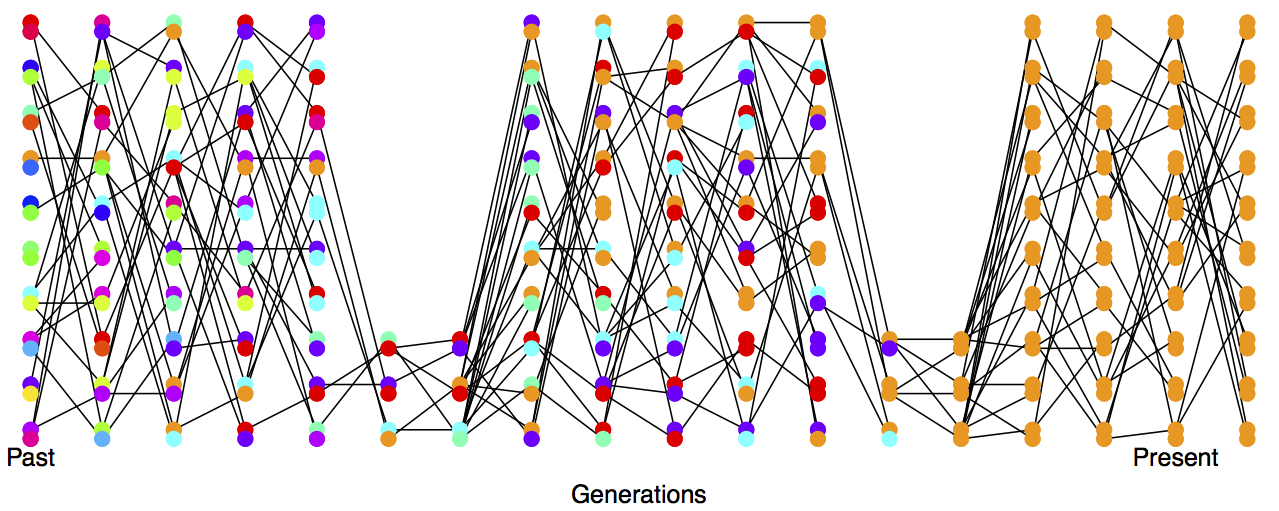
\includegraphics[width= \textwidth]{figures/Loss_of_he_col_alleles_varying_pop_dark.png}
\end{center}
\caption{Loss of heterozygosity over time in a bottlenecking population. A diploid population of 10 individuals, that bottlenecks
  down to three individuals repeatedly. In the first generation I colour every allele a different
colour so we can track their descendants, there are no new
  mutations.} \label{fig:LossHet_varying_pop}  
\end{figure} 

%would result in the same rate of drift
%Luckily, in many (not all) situations, departures from model assumptions can be captured by substituting Ne for N, i.e., by plugging in a fictitious N that leads to the same level of genetic drift as observed.

Variance in reproductive success will also affect our effective
population size. Even if our population has a large constant size of $N$
individuals, if only small proportion of them get to reproduce then
the rate of drift will reflect this much small number of reproducing
individuals. See Figure \ref{fig:LossHet_varying_RS} for a depiction of the higher rate of drift
in a population where there is high variance in reproductive success.

 If only $N_M$ males get to contribute to the next
generation and $N_F$ females get to contribute to the next
generation. When our two alleles pick an ancestor, $25\%$ of the time
our alleles were both in a female ancestor in which case they coalesce
with probability $1/(2N_F)$, and $25\%$ of the time they are both in a
male ancestor in which case they coalesce with probability
$1/(2N_M)$. The remaining $50\%$ of the time our ancestral lineages
are in two individuals are different sexes in a generation so cannot
coalescence.  Therefore, our probability of coalescence in the preceding
generation is
\begin{equation}
\frac{1}{4}\frac{1}{2N_M}+\frac{1}{4}\frac{1}{2N_F} =
\frac{1}{8}\frac{N_F+N_M}{N_FN_M} 
\end{equation}
i.e. the rate of coalescence is the harmonic mean of the two
sexes population sizes, 
equating this to $\frac{1}{2N_e}$ we find
\begin{equation}
N_e = \frac{4N_FN_M}{N_F+N_M}
\end{equation}
Thus if reproductive success is very skewed in one sex (e.g. $N_M \ll
N/2$) our effective population size will be much reduced as a result.\\


\begin{figure}
\begin{center}
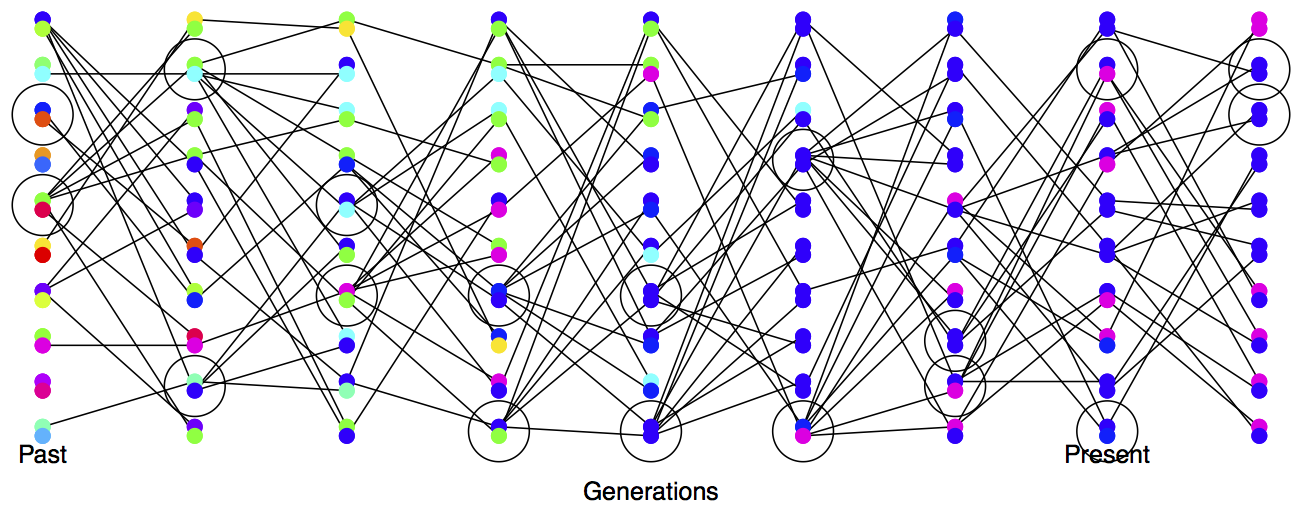
\includegraphics[width= \textwidth]{figures/Loss_of_he_col_alleles_varying_RS.png}

\end{center}
\caption{High variance on reproductive success increases the rate of genetic drift. A diploid population of 10 individuals, where the circled
  individuals have much higher reproductive success. In the first generation I colour every allele a different
colour so we can track their descendants, there are no new
  mutations.} \label{fig:LossHet_varying_RS}
\end{figure} 


\subsection{The Coalescent and patterns of neutral diversity}

\paragraph{Pairwise Coalescent time distribution and the number of
 pairwise differences.}
Thinking back to our calculations we made about the loss of neutral heterozygosity
and equilibrium levels of diversity (in Sections \ref{LossofHet} and \ref{DriftMutationBalance}), you'll note that we could first specify
what generation a pair of sequences coalesce in, and then calculate
some properties of heterozygosity based on that. That's because neutral
mutations do not affect the probability that an individual transmits
that allele, so don't affect the way in which we can trace ancestral lineages
back. \\

As such it will often be helpful to consider the time to the common
ancestor of a pair of sequences, and then think of the impact of that
on patterns of diversity. See Figure \ref{fig:Coalescent_simulation}
for an example of this. The probability that a pair of alleles
have failed to coalesce in $t$ generations and then coalesce in the
$t+1$ generation back is
\begin{equation}
  \frac{1}{2N} \left(1- \frac{1}{2N} \right)^{t} \approx \frac{1}{2N} e^{-t/(2N)} \label{eqn:coal_time_dist}
\end{equation}
thus the coalescent time of a pair of sequences ($T_2$) is
approximately exponentially distributed with a rate $1/(2N)$. We'll denote that by
saying that $T_2 \sim \text{Exp}\left( 1/(2N) \right)$. The mean coalescent
time of a pair of a pair of alleles is $2N$ generations\\


\begin{figure}
\begin{center}
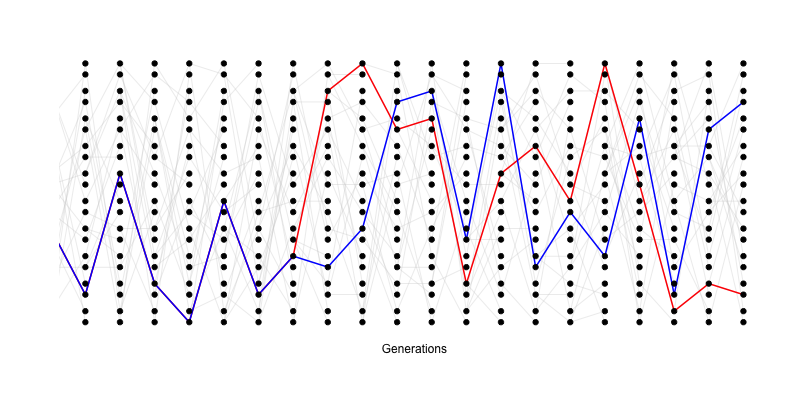
\includegraphics[width=\textwidth]{figures/Coalescent.png}
\end{center}
\caption{A simple simulation of the coalescent process. The simulation
  consists of a diploid population of 10 individuals (20 alleles). In
  each generation, each individual is equally likely to be the parent
  of an offspring (and the allele transmitted is indicated by a light
  grey line).  We track a
  pair of alleles, chosen in the present day, back 14 generations
  untill they find a common ancestor.} \label{fig:Coalescent_simulation}
\end{figure}



Conditional on a pair of alleles coalescing $t$ generations ago
there are $2t$ generations in which a mutation could occur. Thus the
probability of our pair of alleles are separated by $j$ mutations
since they last shared a common ancestor is
\begin{equation}
P(j | T_2 = t ) = {2t \choose j} \mu^{j} (1-\mu)^{2t-j}
\end{equation}
i.e. mutations happen in $j$ generations, and do not happen in $2t-j$
generations (with ${2t \choose j}$ ways this can possibly
happen). Assuming that $\mu \ll 1$, and that $2t-j \approx 2t$ then we
can approximate the probability that we have $j$ mutations as a
Poisson distribution
\begin{equation}
P(j | T_2 = t ) = \frac{ (2 \mu t )^{j} e^{-2\mu t}}{j!}
\end{equation}
i.e. a Poisson with mean $2\mu t $. \\

As our expected coalescent time is $2N$ generations (which follows from the expected value of exponential distributions), the expected
number of mutations separating two alleles drawn at random from the
population is
%
\begin{align}
  \E(j) &= 2\mu\E(t) \\ \nonumber
  &= 4N\mu \\
  &= \theta \nonumber
\end{align}
We'll assume that mutations never happen at the same site twice,
i.e. no multiple hits, such that we get to see all of the mutation events that separate our pair
of sequences (we'll call this the infinitely-many-sites assumption,
which should be fine if $N\mu_{BP} \ll 1$, where $\mu_{BP}$ is the mutation rate per base pair). Thus the number of
mutations between a pair of sites is the observed number of
differences between a pair of sequences. \\

We'll denote the observed number of pairwise differences at putatively neutral
sites separating a pair of sequences as $\pi$ (we usually average this over a
number of pairs of sequences for a region). So we can estimate of $\theta$ from
$\pi$, $\widehat{\theta}_{\pi}$ by setting $\widehat{\theta}_{\pi}=\pi$.  If we
have an independent estimate of $\mu$, then from setting $\pi =
\widehat{\theta}_{\pi} = 4N\mu$ we can obtain an estimate of the population
size $N$ that is consistent with our levels of neutral polymorphism.

\begin{question}
Robinson et al. (Current Biology 2016) report $\pi$ for sample from
populations of the California mainland gray fox and
the San Nicolas Channel Island fox to be 0.0012 and 0.000014
respectively. \\
{\bf A)} How many sites do you expect to differ between two samples
sequenced over a 100kb region in each of these populations?\\   
{\bf B)} Assuming a mutation rate of $2\times 10^{-8}$ what
effective population size do you estimate for these two populations?
\\
{\bf C)} Why is the effective population size of the Channel Island fox
so low? [Hint: quickly google Channel island foxes to read up on their
history, also to see how ridiculously cute they are.]
\end{question}

\subsection{The coalescent process of a sample of alleles.}

Usually we are not just interested pairs of alleles, or the
average pairwise diversity, we are interested in the properties of
diversity in samples of a number of alleles drawn from the population.  
To allow for this instead of just following a pair of lineages back until they
coalesce, we can follow the history of a sample of alleles back
through the population.

Consider first sampling three alleles at random from the population. The
probability that all three alleles choose exactly the same ancestral allele one
generation back is $\nicefrac{1}{(2N)^2}$. If $N$ is reasonably large then this
is a very small probability. As such it is very unlikely that our three alleles
coalesce at once, a in a moment we'll see that it is safe to ignore such
unlikely events. \\

The probability that a specific pair of alleles find a common ancestor in the
preceding generation is still $\nicefrac{1}{(2N)}$. There are three possible pairs of
alleles so the probability that no pair finds a common ancestor is
\begin{equation}
\left(1-\frac{1}{2N} \right)^3 \approx \left( 1- \frac{3}{2N} \right)
\end{equation}
in making this approximation we are multiplying out the right hand-side
and ignoring terms of $1/N^2$ and higher. See
Figure \ref{fig:Coalescent_simulation_3} for a random realization of this process. \\


\begin{figure}
\begin{center}
  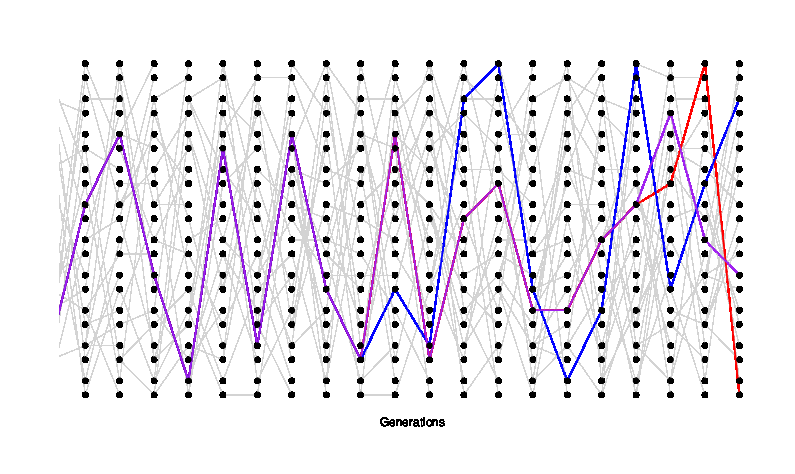
\includegraphics[width = \textwidth]{figures/Coalescent_3.png}
\end{center}
\caption{A simple simulation of the coalescent process for three
  lineages. We track the ancestry of 
  three modern-day alleles, the first pair (blue and purple) coalesce four generations back 
  their are then two independent lineages we are tracking, this pair
  then coalesces twelve generations in the past. Note that different
  random realizations of this process will differ from each other a lot.} \label{fig:Coalescent_simulation_3}
\end{figure}


More generally when we sample $i$ alleles there are ${i \choose
 2}$ pairs, i.e. $i(i-1)/2$ pairs, thus the probability that no pair
of alleles coalesces in the preceding generation is
\begin{equation}
\left(1-\frac{1}{(2N)} \right)^{{i \choose
 2}} \approx \left( 1- \frac{{i \choose
 2}}{2N}\right)
\end{equation}
while the probability of any pair coalescing is $\approx \frac{{i \choose
 2}}{2N}$.\\

We can ignore the possibility of more than pairs of alleles (e.g. tripletons)
simultaneously coalescing at once as terms of $\nicefrac{1}{N^2}$ and higher
can be ignored as they are vanishingly rare. Obviously there are in reasonable
sample sizes there are many more triples (${i \choose 3}$), and higher order
combinations, than pairs (${i \choose 2}$) but if $i \ll N$ then we are safe to
ignore these terms.

When there are $i$ alleles the probability that we wait until the
$t+1$ generation before
any pair of alleles coalesce is
\begin{equation}
 \frac{{i \choose
 2}}{2N}\left( 1- \frac{{i \choose
 2}}{2N}\right)^{t} \approx  \frac{{i \choose
 2}}{2N} \exp \left( - \frac{{i \choose
 2}}{2N} t \right)
\end{equation}
thus the waiting time $T_i$ to the first coalescent event in a sample
of $i$ alleles is exponentially distributed with rate $\frac{{i \choose
2}}{2N}$, i.e. $T_i \sim \text{Exp}\left(\nicefrac{{i \choose
 2}}{2N} \right)$. The mean waiting time till any of pair within our
 sample to coalesce is $\nicefrac{2N}{{i \choose
 2}}$.\\

When a pair of alleles first find a common ancestral allele some
number of generations back further into the past we only have to keep
track of that common ancestral allele for the pair. Thus when a pair
of alleles in our sample of $i$ alleles coalesce, we then switch to
having to follow $i-1$ alleles back. Then when a pair of these $i-1$
alleles coalesce, we then have to follow $i-2$ alleles back. This
process continues until we coalesce back to a sample of two, and from
there to a single most recent common ancestor (MRCA).\\


To simulate a coalescent genealogy at a locus for a sample of $n$ alleles we therefore simply follow this
algorithm
\begin{enumerate}
\item Set $i=n$.
\item We simulate a random variable to be the time $t_i$ to the next coalescent event from $t_i \sim
  \text{Exp}\left(\nicefrac{{i \choose
 2}}{2N} \right)$
\item Choose a pair of alleles to coalesce at random from all possible
 pairs.
\item Set $i=i-1$
\item Continue looping of steps 1-3 until $i=1$ i.e. the most recent
 common ancestor of the sample is found.
\end{enumerate}
by following this algorithm we are generating realizations of the
genealogy of our sample. \\

We will first consider the time to the most recent common ancestor of
the entire sample ($T_{MRCA}$). This is
\begin{equation}
T_{MRCA} = \sum_{i=n}^2 T_i
\end{equation}
generations back. As our coalescent times for different $i$ are independent, the expected time to the most recent common ancestor
is
\begin{equation}
\E(T_{MRCA}) = \sum_{i=n}^2 \E(T_i) = \sum_{i=n}^2  2N/{i \choose
 2}
\end{equation}
using the fact that $\frac{1}{i(i-1)}=\frac{1}{i-1} - \frac{1}{i}$ with a bit of
rearrangement we can rewrite this is
\begin{equation} 
\E(T_{MRCA}) = 4N\left(1- \frac{1}{n} \right) \label{TMRCA_neutral}
\end{equation}
so the average $T_{MRCA}$ scales linearly with population
size. Interestingly, as we move to larger and larger samples (i.e. $n \gg 1$) the average
time to the most recent common ancestor is converging on $4N$. What's
happening here is that in large samples our lineages typically coalesce rapidly
at the start and very soon coalesce down to a much smaller number of
lineages.   \\


%%point about the fixation time of a neutral allele

\paragraph{The total amount of time in a genealogy}

Mutations fall on lineages of the coalescent genealogy. These mutations affect all
descendants of this lineage, and under the infinitely-many-sites assumption,
create a new segregating site for each new mutation. The mutation process is a
\emph{Poisson process}, and the longer a particular lineage branch, the more
mutations that can accumulate on it. The total number of segregating sites in
the genealogy is thus a function of the \emph{total} amount of time in the
genealogy of the sample, or the sum of all the genealogy branch lengths,
$T_{tot}$. Since our coalescent genealogies are bifurcating (only two lineages
coalesce at once), our total amount of time in the genealogy is:

\begin{equation}
T_{tot} = \sum_{i=n}^2 iT_i
\end{equation}
as when there are $i$ lineages each contributes a time $T_i$ to the
total time. Taking the expectation of the total time in the genealogy
\begin{equation}
\E(T_{tot}) = \sum_{i=n}^2 i \frac{2N}{{i \choose
 2} } = \sum_{i=n}^2 \frac{4N}{i -1} =\sum_{i=n-1}^1 \frac{4N}{i}
\end{equation}
so our expected total amount of time in the genealogy scales linearly
with our population size. Our expected total amount of time is also
increasing with sample size but is doing so very slowly. To see this
more carefully we can see that for large $n$
\begin{equation}
\E(T_{tot}) = \sum_{i=n-1}^1 \frac{4N}{i} \approx 4N \int_1^n \frac{1}{i} di
= 4N \log(n-1)
\end{equation}
here we are approximating our sum by an integral, which will work for
large $n$. So our expected total amount of time in the genealogy
is growing with $n$ but it is doing so very slowly. This again follows
from the fact that in large samples the initial coalescence usually
happens very rapidly, so that extra samples adds little to the total
amount of time in the tree. \\

We saw above that the number of mutational differences between a pair
of alleles that coalescence $T_2$ generations ago was Poisson with a
mean of $2 \mu T_2$. A mutation that occurs on any branch of our
genealogy will cause a segregating polymorphism in the sample
(making our infinitely-many-sites assumption). Thus if the total time
in the genealogy is $T_{tot}$ there is $T_{tot}$
generations for mutations. So the total number of mutations
segregating in our sample ($S$) is Poisson with mean $\mu T_{tot}$. Thus the
expected number of segregating  in history a sample of size $n$ is
\begin{equation}
\E(S) = \mu \E(T_{tot}) = \sum_{i=n-1}^1 \frac{4N\mu }{i} = \theta
\sum_{i=n-1}^1 \frac{1}{i}
\end{equation}
Thus we can use this formula to derive another estimate of the
population scaled mutation rate, by setting our observed number of
segregating sites in a sample ($S$) equal to this expectation. We'll call this estimator $\widehat{\theta}_W$
\begin{equation}
\widehat{\theta}_W =\frac{ S}{\sum_{i=n-1}^1 \frac{1}{i}}  
\end{equation}
this estimator was devised by Watterson, hence the $W$.


\subsection{The fixation of neutral alleles} It is very unlikely that a rare
neutral allele accidentally drifts up to fixation; more likely, such an allele
will be eventually lost from the population. However, populations experience a
large and constant influx of rare alleles due to mutation, so even if it is
very unlikely that an individual allele fixes within the population, some
neutral alleles will fix.  \\

%We'll first consider the probability that a neutral allele fixes
%within the population, starting from it just enters a diploid
%population as a newly mutated allele at frequency $1/(2N)$.

%so for an allele to be fixed in the population it
%must have been that allele


\paragraph{Probability of the eventual fixation of a neutral allele}
% TODO: tried to clean up this section, needs more work
An allele which reaches fixation within a population is an ancestor to the
entire population. In a particular generation there can be only single allele
that all other alleles at the locus in later generation can claim as an
ancestor. A neutral locus, the actual allele does not affect the number of
descendents that the allele has (this follows from the definition of
neutrality: neutral alleles don't leave more or less descendents on average).
An equivalent way to state this is that the allele labels don't affect
anything; thus the alleles are \emph{exchangeable}. As a consequence of this,
any allele is equally likely to be the ancestor of the entire population.  In a
diploid population size of size $N$, there are $2N$ alleles all of which are
equally likely to be the ancestor of the entire population at some later time
point. So if our allele is present in a single copy, the chance that it is the
ancestor to the entire population in some future generation is
$\nicefrac{1}{(2N)}$, i.e. the chance our neutral allele is eventually fixed is
$\nicefrac{1}{(2N)}$.  See Figure \ref{fig:subs_simulation}, our orange allele
in the first generation is one of 10 differently coloured alleles, and so has a
$1/10$ chance of being the ancestor of the entire population at some later time
point (as it is by the 9th generation).\\

More generally if our neutral allele is present in $i$ copies in the
population, of $2N$ alleles, the probability that this allele is fixed is
$\nicefrac{i}{(2N)}$, i.e. the probability that a neutral allele is eventually
fixed is simply given by its frequency ($p$) in the population.  We can also
derive this result by letting $Ns \rightarrow 0$ in eqn.
\eqref{eqn:prob_fixed}.

\begin{figure}
\begin{center}
  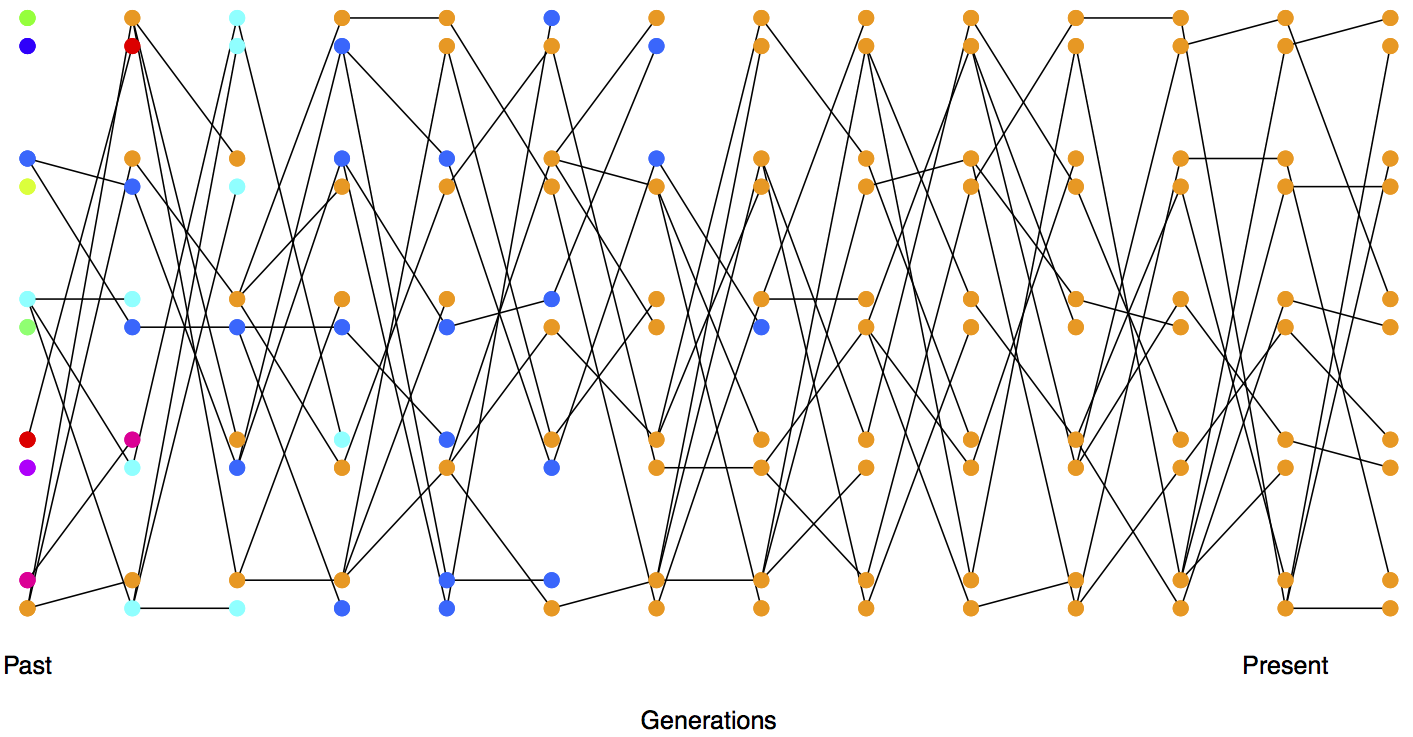
\includegraphics[width = \textwidth]{figures/Substitution_sim.png}
\end{center}
\caption{Each allele initially present in a small diploid population is
  given a different colour so we can track their descendants over
  time. By the 9th generation all of the alleles present in the
  population can trace their ancestry back to the orange allele.} \label{fig:subs_simulation}
\end{figure}


% TODO
An allele newly arisen mutation only becomes a fixed difference if it is lucky
enough to be the ancestor of the entire population. As we saw above this occurs
with probability $\nicefrac{1}{(2N)}$. How long does is take on average for
such an allele to fix within our population? Well in developing
equation \eqref{TMRCA_neutral} we've seen that it takes $4N$
generations for a large sample of alleles to all trace their ancestry back to a
single most recent common ancestor. Thus it must take roughly $4N$ generations
for a neutral allele present in a single copy within the population to the
ancestor of all alleles within our population. This argument can be made more
precise, but in general we would still find that it takes $\approx 4N$
generations for a neutral allele to go from its introduction to fixation with
the population.   \\


\paragraph{Rate of substitution of neutral alleles}

A substitution between populations that do not exchange gene flow is simply a
fixation event within one population. The rate of substitution is therefore the
rate at which new alleles fix in the population, so that the long-term
substitution rate is the rate at which mutations arise that will eventually
become fixed within our population.\\

Assume that there are two classes of mutational changes that can occur with a
region, highly deleterious mutations and neutral mutations. A fraction $C$ of
all mutational changes are highly deleterious, and can not possibly contribute
to substitution nor polymorphism (i.e. $Ns \gg 1$).  The other $1-C$ fraction
of mutations are neutral. If our mutation rate is $\mu$ per transmitted allele
per generation, then a total of $2N \mu (1-C)$ neutral mutations enter our
population each generation.\\

Each of these neutral mutations has a $\nicefrac{1}{(2N)}$ probability chance of
eventually becoming fixed in the population. Therefore, the rate at
which neutral mutations arise that eventually become fixed within our
population is  
\begin{equation}
2N\mu(1-C)\frac{1}{2N} = \mu(1-C)
\end{equation}
thus the rate of substitution under a model where newly arising alleles are either
highly deleterious or neutral, is simply given by the mutation rate
towards neutral alleles, i.e. $\mu(1-C)$.\\

Consider a pair of species have diverged for $T$ generations, i.e. orthologous sequences shared between the species last shared a common ancestor $T$ generations ago. If they have maintained a constant $\mu$ over that time, will have accumulated an average of
\begin{equation}
2\mu(1-C)T
\end{equation}
neutral substitutions. This assumes that $T$ is a lot longer than the time it
takes to fix a neutral allele, such that the total number of 
alleles introduced into the population that will eventually fix is the
total number of substitutions. We'll see below that a neutral allele
takes on average $4N$ generations to fix from its introduction into
the population.\\

This is a really pretty result as the population size has completely canceled
out of the neutral substitution rate. However, there is another way to see this
in a more straight forward way. If I look at a sequence in me compared to say a
particular chimp, I'm looking at the mutations that have occurred in both of
our germlines since they parted ways $T$ generations ago. Since neutral alleles
do not alter the probability of their transmission to the next generation, we
are simply looking at the mutations that have occurred in $2T$ generations
worth of transmissions. Thus the average number of neutral mutational
differences separating our pair of species is simply $2\mu (1-C) T$.\\

\begin{question}
For this, and the next question, assume that humans and chimp diverged
around 5.5$\times 10^6$ years, a generation time ~20 years, that the speciation occurred instantaneously in allopatry with no subsequent gene flow, and the ancestral effective population size of the human and chimp common ancestor population was 10,000 individuals.\\
Nachman and Crowell sequenced 12 pseudogenes in human and chimp found substitutions at 1.3\% of sites. \\
{\bf A) } What can you say about the mutation rate per site per generation at these genes, and how does it compare to other estimates of human mutation rate?\\
{\bf B)} All of the pseudogenes they sequenced are on the autosomes. What
would you prediction be for pseudogenes on the X and Y chromosomes,
given that there are fewer rounds of replication in the female
germline than in the male germline.
\end{question}




\subsection{Neutral diversity and population structure}
%%this section was moved from the coalescent chapter
Up to now we have assumed that our alleles that we have modelled in the
coalescent setting are drawn from a randomly mating population such
that any pair of lineages is equally likely to coalesce with each
other. However, when there is population structure this assumption is
violated. \\

We have previously written the measure of population structure
$\fst$ as
\begin{equation}
\fst = \frac{H_T-H_S}{H_T}
\end{equation}
where $H_S$ is the probability that two alleles sampled at random from a
subpopulation differ, and $H_T$ is the probability that two alleles
sampled at random from the total population differ. 

\paragraph{A simple population split model}
Imagine a population of constant size of $N_e$ diploid individuals that
$\tau$ generations in the past split into two daughter populations (sub-populations)
each of size $N_e$ individuals, who do not subsequently exchange
migrants. In the current day we sample an equal number of alleles
from both subpopulations.

Consider a pair of alleles sampled within one of our
sub-populations, they have experienced a population of size $N_e$
and so the probability that they differ is $H_S = \theta/(1+\theta)$
(where $\theta=4N_e\mu$).
The heterozygosity in our total population is a little more tricky to
calculate. Assuming that we equally sample both sub-populations, when we draw two alleles from our total
sample, $50\%$ of the time they are drawn from the same
subpopulation and $50\%$ of the time they are drawn from different
subpopulations. Therefore, our total heterozygosity is given by
\begin{equation}
H_T = \half H_S + \half H_B
\end{equation}
where $H_B$ is the probability that a pair of alleles drawn from our
two different sub-populations differ from each other. Our pair of
alleles can not find a common ancestor with each other for at least $\tau$
generations into he past as they are in distinct populations (not
connected by migration). The probability that one or other of them
mutates in this time is $1-(1-\mu)^{2T}$. With probability
$(1-\mu)^{2T} $ neither of our alleles mutate in the $T$ generations
back in time before they find themselves back in the combined ancestral 
population. Conditional on failing to mutate before the combined ancestral
population, the probability that they do manage to mutate before
coalescing in that population of size $N_e$ is
$\theta/(\theta+1)$. Putting these components together
\begin{equation}
H_B = \left( 1-(1-\mu)^{2T} \right) + (1-\mu)^{2T}
  \frac{\theta}{\theta+1} 
\end{equation}
We can plug this into our expression for $H_T$, and then that in turn
into $\fst$.

\begin{figure}
\begin{center}
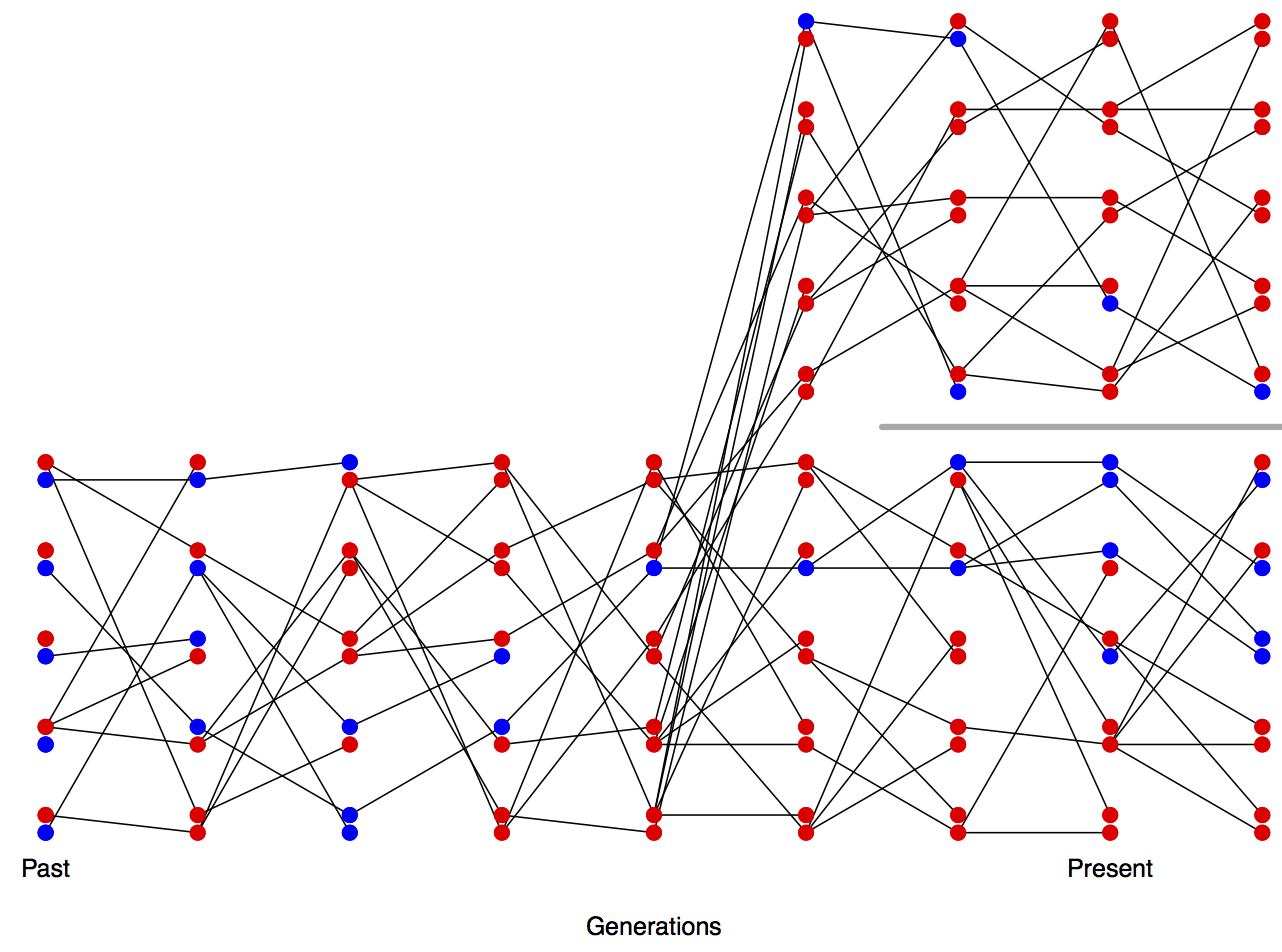
\includegraphics[width= 0.8 \textwidth]{figures/drift_split.png}
\end{center}
\caption{Change in allele frequencies following a population split.} \label{fig:drift_split}  
\end{figure} 

To understand this better we can make a simple
approximation based on our mutation rate being very low, such that
$N_e \mu \ll 1$ so $H_S \approx
4N_e\mu$, and that $\mu \ll 1$ and $\mu T \ll 1$. Assuming this, then  
\begin{equation}
H_B \approx 2 \mu T + 4N_e\mu. 
\end{equation}
So that 
\begin{equation}
\fst \approx \frac{ \mu T}{\mu T +  4N_e\mu }  %= \frac{ T}{ T +  4N_e }
\end{equation}
note that $\mu$ cancels out of this. In this simple toy model $\fst$
is increasing because the amount of between population diversity 
increases with the divergence time of the two populations (initially
linearly with $T$). It does so at a rate
give by $\nicefrac{T}{(4N_e)}$ so that differentiation will be higher
between populations separated by long divergence times or with small
effective population sizes.

\begin{question}
The gorilla lineage split from the human-chimp lineage $\sim$7 million years ago. Let’s assume that this speciation event occurred instantaneously in allopatry with no subsequent gene flow. \\
{\bf A)}	What is the probability of that gorilla is not an outgroup to human and chimp at a single locus?\\
{\bf B)}	It has been estimated that the gorilla lineage is not an outgroup at around ~30\% of autosomal loci. What effective population size would you need to assume to explain this observation? Is that only plausible explanation?\\
{\bf C)}	The gorilla lineage is an outgroup for large portions of the X chromosome, what is a plausible explanation for this finding?
\end{question}

\paragraph{A simple model of migration between an island and the mainland.}
We can also use the coalescent to think about patterns of
differentiation under a simple model of migration drift
equilibrium. Lets consider a small island population that is relatively isolated
from a large mainland population, and that both of these populations
are constant in size. We'll assume that the expected heterozygosity
for a pair of alleles sampled on the mainland is $H_M$.

Our island has a population size
$N_{I}$ that is very small compared to our mainland population.
Each generation some low fraction $m$ of our individuals on the
island have migrant parents from the mainland the generation
before. Our island may also send migrants back to the mainland, but
these are a drop in the ocean compared to the large population size on
the mainland and their effect can be ignored. 


If we sample an allele on the island back and trace its ancestral
lineage backward in time, each generation our ancestral allele have a low
probability $m$ of being descended from the mainland in the proceeding
generation (if we go far enough the allele eventually has to be
descended from an allele on the mainland). The probability that a pair of alleles sampled on the
island are descended from a shared recent common ancestral allele on the island, is the
probability that our pair of alleles coalesce before either lineage
migrates. For example, the probability that our pair of alleles
coalesce $t+1$ generations back is 
\begin{equation}
\frac{1}{2N_I}(1-m)^{2(t+1)} \left(1-\frac{1}{2N_I} \right)^{t} \approx
\frac{1}{2N_I} \exp\left( -t\left (\frac{1}{2N_I} + 2m\right) \right),
\end{equation}
with the approximation following from assuming that $m \ll 1$ \& $\frac{1}{(2N_I)}
\ll 1$ (note that this is very similar to our derivation of
heterozygosity above). The probability that our alleles coalescence before either one
of them migrates off the island, irrespective of the time, is
\begin{equation}
\int_0^{\infty} \frac{1}{2N_I} \exp\left( -t\left (\frac{1}{2N_I} +
2m\right) \right) dt = \frac{\nicefrac{1}{(2N_I)}}{\nicefrac{1}{(2N_I)} +
    2m}.
\end{equation}

Lets assume that the mutation rate is very low such as it is very
unlikely that the pair of alleles mutate before they coalesce on the
island. Therefore, the only way that the alleles can be different from
each other is if one or other of them migrates to the mainland, which
happens with probability  
\begin{equation}
  1 - \frac{\nicefrac{1}{(2N_I)}}{\nicefrac{1}{(2N_I)} + 2m}
\end{equation}
Conditional on one or other of our alleles migrating to the mainland,
both of our alleles represent independent draws from the mainland and
so differ from each other with probability $H_M$. Therefore, the level of
heterozygosity on the island is given by
\begin{equation}
  H_I = (1 - \frac{\nicefrac{1}{(2N_I)}}{1/(2N_I) + 2m})H_M
\end{equation}
So the reduction of heterozygosity on the island compared to the
mainland is
\begin{equation}
  F_{IM} = 1- \frac{H_I}{H_M} = \frac{\nicefrac{ 1}{(2N_I)}}{\nicefrac{1}{(2N_I)} + 2m} = \frac{ 1 }{1 + 4N_Im}.
\end{equation}
The level of inbreeding on the island compared to the mainland will
be high in the migration rate is low and the effective population size
of the island is low, as allele frequencies on the island are drifting
and diversity is not being replenished on the island by migration. The
key parameter here is the number individuals on the island replaced by
immigrants from the mainland each generation ($N_I m$).

We have framed this as being about the reduction in genetic diversity on the
island compared to the mainland. However, if we consider collecting 
individuals on the island and mainland in proportion to population
sizes the total level of heterozygosity would be $H_T=H_M$, as samples
from our mainland would greatly outnumber those from our
island. Therefore, considering our island our sub-population we have
derived another simple model of $F_{ST}$.

\begin{question}
You are investigating a small river population of sticklebacks, which receives infrequent migrants from a very large marine population. At a set of (putatively neutral biallelic markers the freshwater population has frequencies:\\
0.2, 0.7, 0.8\\
at the same markers the marine population has frequencies:\\
0.4, 0.5 and 0.7.\\
 From studying patterns of heterozygosity at a large collection of markers, you have estimated the long term effective size of your freshwater population is 2000 individuals.\\
What is your estimate of the migration rate from the marine
populations into the river?
\end{question}
\newpage


%\section{Correlations between loci, linkage disequilibrium, and recombination}

%</source-file>

Up to now we have been interested in correlations between alleles at the
same locus, e.g. correlations within individuals (inbreeding) or between
individuals (relatedness). We have seen how relatedness between parents affects the extent to which their offspring is inbred. We now turn to 
correlations between alleles at different loci. To understand
correlations between loci we need to understand recombination.\\


\paragraph{Recombination}  Lets
consider an individual heterozygous for a $AB$ and $ab$
haplotype. If no recombination occurs between our two loci in this
individual, then these two haplotypes will be transmitted intact to
the next generation. While if a recombination (or more generally an
odd number of recombinations) occurs between our two loci on the
haplotype transmitted to the child then $\tfrac{1}{2}$ the time the
child receives a $Ab$ haplotype and $\tfrac{1}{2}$ the time the child
receives a $aB$ haplotype. So recombination is breaking up the
association between loci. We'll define the recombination fraction ($r$) to be
the probability of an odd number of recombinations between our loci.
In practice we'll often be interested in relatively short regions
where recombination is relatively rare, and so we might think that
$r=r_{BP}L \ll 1$, where $r_{BP}$ is the average recombination rate
per base pair (typically $\sim 10^{-8}$) and L is the number of base
pairs separating our two loci.\\



\paragraph{Linkage disequilibrium}
The (horrible) phrase linkage
disequilibrium (LD) refers to the statistical non-independence
(i.e. a correlation)  of
alleles at different loci. Our two loci, which segregate alleles $A/a$ and $B/b$, have allele
frequencies of $p_A$ and $p_B$ respectively. The frequency of the two locus haplotype is $p_{AB}$,
and likewise for our other three combinations. If our loci were
statistically independent then $p_{AB} = p_Ap_B$, otherwise $p_{AB} \neq p_Ap_B$
We can define a covariance between the $A$ and $B$ alleles at our two loci as
\begin{equation}
D_{AB} = p_{AB} - p_Ap_B
\end{equation}
and likewise for our other combinations at our two loci
($D_{Ab},~D_{aB},~D_{ab}$). These $D$ statistics are all closely
related to each other as $D_{AB} = - D_{Ab}$ and so on. Thus we only
need to specify one $D_{AB}$ to know them all, so we'll drop the
subscript and just refer to $D$. Also a handy result is that we can rewrite our haplotype
frequency $p_{AB}$ as
\begin{equation}
p_{AB} = p_Ap_B+D. \label{eqn:ABviaD}
\end{equation}
If $D=0$ we'll say the two loci are in linkage equilibrium, while if
$D>0$ or $D<0$ we'll say that the loci are in linkage
disequilibrium (we'll perhaps want to test whether $D$ is
statistically different from $0$ before making this choice). You should be careful to keep the concepts of linkage
and linkage disequilibrium separate in your mind. Genetic linkage refers to the
linkage of multiple loci due to the fact that they
are transmitted through meiosis together (most often because the
loci are on the same chromosome). Linkage disequilibrium merely refers
to the correlation between the alleles at different loci, this may in
part be due to the genetic linkage of these loci but does not
necessarily imply this (e.g. genetically unlinked loci can be in LD
due to population structure). \\

Another common statistic for summarizing LD is $r^2$ which we write as
\begin{equation}
r^2 = \frac{D^2}{p_A(1-p_A) p_B(1-p_B) }
\end{equation}
as $D$ is a covariance, and $p_A(1-p_A) $ is the variance of an allele
drawn at random from locus $A$, $r^2$ is the squared correlation
coefficient.    \\


{\bf Question.} You genotype 2 bi-allelic loci (A \& B) segregating in two mouse subspecies (1 \& 2) which mate randomly among themselves, but have not historically interbreed since they speciated. On the basis of previous work you estimate that the two loci are separated by a recombination fraction of 0.1. The frequencies of haplotypes in each population are:
\begin{center}
\begin{tabular}{|c|cccc|}
\hline
Pop    & $p_{AB}$    & $p_{Ab}$ &    $p_{aB}$ &    $p_{ab}$\\
\hline
1 &    .02    & .18 &     .08 &    .72\\
2&    .72 &    .18 &    .08 &    .02\\
\hline
\end{tabular}
\end{center}

{\bf A)} How much LD is there within populations, i.e. estimate D?\\

{\bf B)} If we mixed the two populations together in equal proportions what value would D take before any mating has had the chance to occur? \\



\paragraph{The decay of LD due to recombination}
We will now examine what happens to LD over the generations if we
only allow recombination to occur in a very large population (i.e. no
genetic drift, i.e. the frequencies of our loci follow their expectations). To do so consider the frequency of our $AB$ haplotype in the next generation
$p_{AB}^{\prime}$. We lose a fraction $r$ of our $AB$ haplotypes to
recombination ripping our alleles apart but gain a fraction $rp_A p_B$ per generation from other
haplotypes recombining together to form $AB$ haplotypes. Thus in the
next generation
\begin{equation}
p_{AB}^{\prime} = (1-r)p_{AB} + rp_Ap_B
\end{equation}
this last term here is $r(p_{AB}+p_{Ab})(p_{AB}+p_{aB})$, which
multiplying this out is the
probability of recombination in the different diploid genotypes that
could generate a $p_{AB}$ haplotype. \\

We can then write the change in the frequency of the $p_{AB}$
haplotype as
\begin{equation}
\Delta p_{AB} = p_{AB}^{\prime} -p_{AB} = -r p_{AB} + rp_Ap_B = - r D
\end{equation}
so recombination will cause a decrease in the frequency of $p_{AB}$ if
there is an excess of $AB$ haplotypes within the population ($D>0$), and an
increase if there is a deficit of $AB$ haplotypes within the
population ($D<0$). Our LD in the next generation is $D^{\prime} =
p_{AB}^{\prime}$, so we can rewrite the above eqn. in terms of the
$D^{\prime} $
\begin{equation}
D^{\prime}= (1-r) D
\end{equation}
so if the level of LD in generation $0$ is $D_0$ the level $t$
generations later ($D_t$) is
\begin{equation}
D_t=  (1-r)^t D_0
\end{equation}
so recombination is acting to decrease LD, and it does so
geometrically at a rate given by $(1-r)$. If $r \ll 1$ then we can
approximate this by an exponential and say that   
\begin{equation}
D_t \approx  D_0 e^{-rt}
\end{equation}\\



{\bf Q C)} You find a hybrid population between the two mouse subspecies
described in the question above, which appears to be comprised of equal proportions of ancestry from the two subspecies.  You estimate LD between the two markers to be 0.0723. Assuming that this hybrid population is large and was formed by a single mixture event, can you estimate how long ago this population formed? \\

%\subsection{Testing for departures from HWE.}
%Note the form of $\hat{F}$ \eqref{eqn:FhatHO} is the same as the $X^2$
%statistic, and so we can test for a deviation from hardy-weinberg  $X^2$


%\subsection{Population structure}
%The question naturally arises at this point: what reference population
%(i.e. what allele frequency) do we use to calculate $\hat{F}$? If we are %calculating the inbreeding coefficient
%of an English person do we use the frequencies of the town of that
%person, of England, of the United Kingdom, or of the World?



%\gc{Include the HapMap exercise here?}


%==One locus models of selection==
%<source-file filename="one_loc_sel_models.tex" display="one_loc_sel_models.wrapped.latexml.xhtml">

\newpage


\section{The phenotypic resemblance between relatives}

We can use our understanding of the sharing of alleles between relatives
to understand the phenotypic resemblance between relatives in
quantitative phenotypes. We can then use this to understand the
evolutionary change in quantitative phenotypes in response to selection. \\

\subsection{A simple additive model of a trait}
Let's imagine that the genetic component of the variation in our trait
is controlled by $L$ autosomal loci that act in an additive manner. The frequency of allele $1$ at locus $l$ is $p_l$, with each copy of
allele $1$ at this locus increasing your trait value by $a_l$ above
the population mean.
The phenotype of an individual, let's call her $i$, is $X_i$.
Her genotype at SNP $l$, is
$G_{i,l}$. Here $G_{i,l}=0,~1,$ or $2$  represents the number of copies of allele $1$ she
has at this SNP. Her expected phenotype, given her genotype, is then
\begin{equation}
\E (X_i | G_{i,1},\cdots,G_{i,L}) =\mu + X_{A,i} = \mu+\sum_{l=1}^L G_{i,l} a_{l} \label{pheno_geno}
\end{equation}
where $\mu$ is the mean phenotype in our population, and $X_{A,i}$ is
the deviation away from the mean phenotype due to her genotype. Now in reality the genetic phenotype is a function of the
expression of those alleles in a particular environment. Therefore, we
can think of this expected phenotype as being an average across a set
of environments that occur in the population. \\

%\gc{NEED to resolve $\mu$ in above equation}


When we measure our individual's observed phenotype we see
\begin{equation}
X_i =   \mu+X_{A,i} + X_{E,i} \label{pheno_geno_environ}
\end{equation}
where $X_E$ is the deviation from the mean phenotype due to the
environment. This $X_E$ included the systematic effects of the environment
our individual finds herself in and all of the noise during
development, growth, and the various random insults that life throws
at our individual. If a reasonable number of loci contribute to
variation in our trait then we can approximate the distribution of
$X_{A,i}$ by a normal distribution due to the central limit theorem (see Figure \ref{fig:QT1}). Thus if we can
approximate the distribution of the effect of environmental variation
on our trait ($X_{E,i}$) also by a normal distribution, which is
reasonable as there are many small environmental effects, then the
distribution of phenotypes within the population ($X_i$) will be
normally distributed (see Figure \ref{fig:QT1}).\\

\begin{figure}
\begin{center}
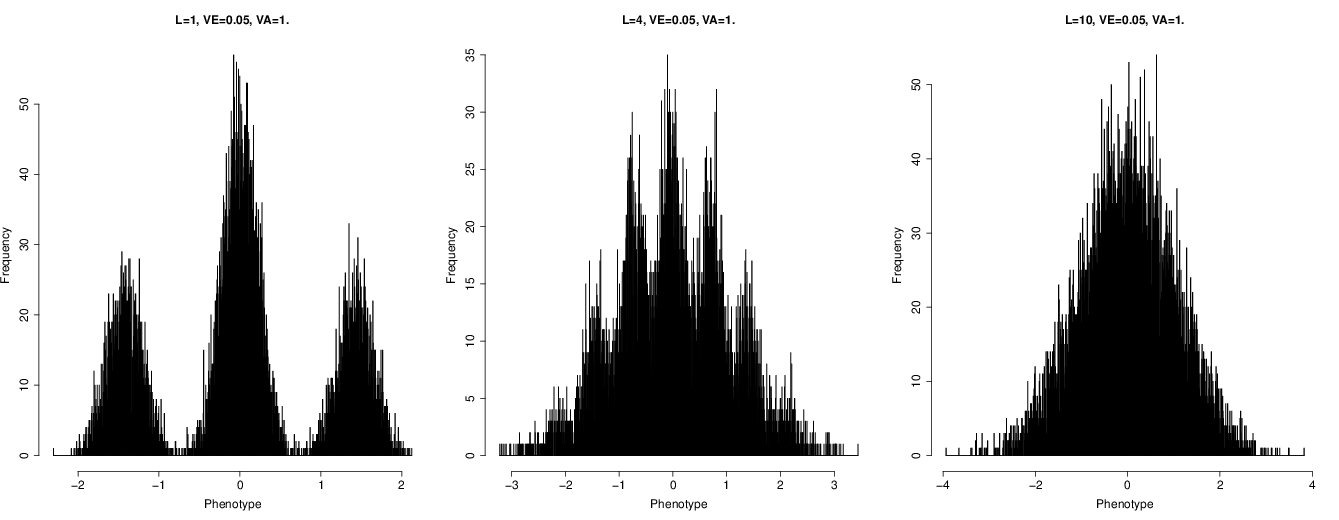
\includegraphics[width=\textwidth]{figures/QT1.png}
\end{center}
\caption{The convergence of the phenotypic distribution to a normal
  distribution. Each of the three histograms shows the distribution of
the phenotype in a large sample, for increasing large numbers of loci ($L$). I have simulated each individual's
phenotype following equation \ref{pheno_geno} and \ref{pheno_geno_environ}. Specifically I simulate each
individuals biallelic genotype at $L$ loci, assuming Hardy-Weinberg proportions
and that the allele is at 50\% frequency. I assume that all of the
alleles have equal effects and combine them additively together. I then
add an environmental contribution, which is normally distributed with
variance $0.05$. Note that in the left two pictures you can see peaks
corresponding to different genotypes.} \label{fig:QT1}
\end{figure}

Note that as this is an additive model we can decompose eqn. \ref{pheno_geno_environ} into the
effects of the two alleles at each locus, in particular we can rewrite
it as
\begin{equation}
X_i = \mu + X_{iM}+X_{iP} +X_{iE}
\end{equation}
where $X_{iM}$ and $X_{iP}$ are the contribution to the phenotype of
the allele that our individual received from her mother (maternal
alleles) and father (paternal alleles) respectively. This will come in
handy in just a moment when we start thinking about the phenotype covariance of relatives.\\

Now obviously this model seems silly at first sight as alleles don't
only act in an additive manner, as they interact with alleles at the
same loci (dominance) and at different loci (epistasis). Later we'll
relax this assumption, 
however, we'll find that if we are interested in evolutionary change
over short time-scales it is actually only the ``additive
component'' of genetic variation that will (usually) concern us. 
We will define this more formally later on, but for the moment 
we can offer the intuition that parents only get to pass on a single
allele at each locus on to the next generation. As such, it is the
effect of these transmitted alleles, averaged over possible matings,
that is an individual's average contribution  to the next generation
(i.e. the additive effect of the alleles that their genotype consists of).



\subsection{Additive genetic variance and heritability}
As we are talking about an additive genetic model we'll talk about the
additive genetic variance ($V_A$), the variance due to the additive
effects of segregating genetic variation. This is a subset of the total genetic
variance if we allow for non-additive effects. \\

The variance of our phenotype across individuals ($V$) can write this as
\begin{equation}
V = Var(X_A) + Var(X_E) = V_A+V_E
\end{equation}
in writing this we are assuming that there is no covariance between $X_{G,i}$
and $X_{E,i}$ i.e. there is no covariance between genotype and
environment. \\

Our additive genetic variance can be written as
\begin{equation}
V_A = \sum_{l=1}^L Var(G_{i,l} a_{l})
\end{equation}
where $Var(G_{i,l} a_{l})$ is the contribution to the additive
variance among individuals of the $l$ locus. Assuming random mating we
can write our additive genetic variance as
\begin{equation}
V_A = \sum_{l=1}^L a_{l}^2 2 p_l(1-p_l)
\end{equation}
where the $ 2 p_l(1-p_l)$ term follows the binomial sampling of two
alleles per individual at each locus. \\

\paragraph{The narrow sense heritability}
We would like a way to think about what proportion of the variation
in our phenotype across individuals is due to genetic differences as
opposed to environmental differences. Such a quantity will be key in
helping us think about the evolution of phenotypes. For example, if
variation in our phenotype had no genetic basis then no matter how
much selection changes the mean phenotype within a generation
the trait will not change over generations. \\

We'll call the proportion of the variance that is genetic the
heritability, and denote it by $h^2$. We can then write this as
\begin{equation}
h^2 = \frac{Var(X_A)}{V} = \frac{V_A}{V}
\end{equation}
remember that we thinking about a trait where all of the alleles act
in a perfectly additive manner. In this case our heritability $h^2$ is
referred to as the narrow sense heritability, the proportion of the
variance explained by the additive effect of our loci.
When we allow dominance
and epistasis into our model we'll also have to define the broad sense
heritability (the total proportion of the phenotypic variance
attributable to genetic variation).\\

The narrow sense heritability of a trait is a useful quantity, indeed
we'll see shortly that it is exactly what we need to understand the
evolutionary response to selection on a quantitative phenotype. We can
calculate the narrow sense heritability by using the resemblance between
relatives. For example, if our phenotype was totally environmental we
should not expect relatives to resemble each other any more than random
individuals drawn from the population. Now the obvious caveat here is
that relatives also share an environment, so may resemble each other
due to shared environmental effects. \\

\subsection{The covariance between relatives}
So we'll go ahead and calculate the covariance in phenotype between two individuals
($1$ and $2$) who have a phenotype $X_1$ and $X_2$ respectively.
\begin{equation}
Cov(X_1,X_2) =
Cov\left((X_{1M}+X_{1P}+X_{1E}),((X_{2M}+X_{2P}+X_{2E}) \right)
\end{equation}
We can expand this out in terms of the covariance between the various
components in these sums.\\

To make our task easier we (and most analyses) will assume two things
\begin{enumerate}
\item that we can ignore the covariance of the environments
between individuals (i.e. $Cov(X_{1E},X_{2E})=0$)
\item that we can ignore the covariance
between the environment variation experience by an individual and the
genetic variation in another individual (i.e. $Cov(X_{1E},(X_{2M}+X_{2P}))=0$).
\end{enumerate}

The failure of these assumptions
to hold can severely undermine our estimates of heritability, but we'll
return to that later. Moving forward with these assumptions, we can
write our phenotypic covariance between our pair of individuals as
\begin{equation}
Cov(X_1,X_2) =
Cov((X_{1M},X_{2M})+Cov(X_{1M},X_{2P})+Cov(X_{1P},X_{2M})
+Cov(X_{1P},X_{2P}) \label{cov_rels_1}
\end{equation}
This is saying that under our simple additive model we can see the
covariance in phenotypes between individuals as the covariance between
the allelic effects in our individuals. We can use our results about
the sharing of alleles between relatives to obtain these terms.
But before we write down the general case lets quickly work through some
examples. \\


\paragraph{The covariance between Identical Twins}
Lets first consider the case of a pair of identical twins from two
unrelated parents. Our pair of twins share their maternal and paternal
allele identical by descent ($X_{1M}=X_{2M}$ and $X_{1P}=X_{2P}$). As their maternal and
paternal alleles are not correlated draws from the population,
i.e. have no probability of being $IBD$ as we've said the parents are unrelated, the
covariance between their effects on the phenotype is zero  
(i.e. $Cov(X_{1P},X_{2M})=Cov(X_{1M},X_{2P})=0$). In that case
eqn. \ref{cov_rels_1} is
\begin{equation}
Cov(X_1,X_2) = Cov((X_{1M},X_{2M})+Cov(X_{1P},X_{2P}) = 2Var(X_{1M})
= V_A
\end{equation}
Now in general identical twins are not going to be super helpful for
us in estimating $h^2$ as under models with non-additive effects
identical twins have higher covariance than we'd expect as they
resemble each other also because of the dominance effects as they
don't just share alleles they share their entire genotype.\\

\paragraph{The covariance in phenotype between mother and child}.
If the mother and father are unrelated individuals (i.e. are two
random draws from the population) then the mother and a child share
one allele IBD at each locus (i.e. $r_1=1$ and $r_0=r_2=0$). Half the
time our mother transmits her paternal allele to the child, in which
case $X_{P1}=X_{M2}$ and so $Cov(X_{P1},X_{M2})=Var(X_{P1})$ and all
the other covariances in eqn. \ref{cov_rels_1} zero, and half
the time she transmits her maternal allele to the child
$Cov(X_{M1},X_{M2})=Var(X_{M1})$ and all the other terms zero. By this
argument $Cov(X_1,X_2) = \half Var(X_{M1}) + \half Var(X_{P1}) = \half
V_A$. \\

\paragraph{The covariance between general pairs of relatives under an
additive model}
The two examples make clear that to understand the covariance between
phenotypes of relatives we simply need to think about the alleles they
share IBD. Consider a pair of relatives ($1$ and $1$) with a probability $r_0$,
$r_1$, and $r_2$ of sharing zero, one, or two alleles IBD
respectively. When they share zero alleles
$Cov((X_{1M}+X_{1P}),(X_{2M}+X_{2P}))=0$, when they share one allele
$Cov((X_{1M}+X_{1P}),(X_{2M}+X_{2P}))=
Var(X_{1M})=\frac{1}{2}V_A$, and when they share two alleles $Cov((X_{1M}+X_{1P}),(X_{2M}+X_{2P}))=
V_A$. Therefore, the general covariance between two
relatives is
\begin{equation}
Cov(X_1,X_2) = r_0 \times 0 + r_1 \frac{1}{2}V_A + r_2  V_A =
2 F_{1,2} V_A  \label{additive_covar_general_rellys}
\end{equation}\\
So under a simple additive model of the genetic basis of a phenotype
to measure the narrow sense heritability we need to measure the
covariance between a set of pairs of relatives (assuming that we can remove the effect of
shared environmental noise). From the covariance between relatives we
can calculate $V_A$, we can then divide this by the total phenotypic
variance to get $h^2$. \\
%One way potentially to get somewhat around the
%shared environmental effect is to use paternal half-sibs as they share a

\begin{tcolorbox}
\begin{question}
{\bf A)} In polygynous blackbird populations (i.e. males mate with
several females), paternal half-sibs can be identified.  Suppose that
the covariance of tarsus lengths among half-sibs is 0.25 $cm^2$ and
that the total phenotypic variance is 4 $cm^2$.  Use these data to
estimate $h^2$ for tarsus length in this population. \\

{\bf B)} Why might paternal half-sibs be preferable for measuring
heritability than maternal half-sibs? 
\end{question}
\end{tcolorbox}

Another way that we can estimate the narrow sense heritability is
through the regression of child's phenotype on the parental mid-point
phenotype. The parental mid-point phenotype is simple the average of
the mum and dad's phenotype. Denoting the child's phenotype by $X_{kid}$ and mid-point
phenotype by $X_{mid}$ so that if we take the regression $X_{kid} \sim X_{mid}$ this
regression has slope $\beta = Cov(X_{kid},X_{mid})/Var(X_{mid})$.
The covariance of $Cov(X_{kid},X_{mid})=\half
V_A$, and $Var(X_{mid}) = \half V$ as by taking the average of the
parents we have halved the variance, such that the slope of the
regression is
\begin{equation}
\beta_{mid,kid}= \frac{Cov(X_{kid},X_{mid})}{Var(X_{mid})} = \frac{V_A}{V} = h^2
\end{equation}
i.e. the regression of the child's phenotype on the parental midpoint
phenotype is an estimate of the narrow sense heritability. This is a
common way to estimate heritability, although it doesn't bypass the
need to control for environmental correlations between relatives. \\

Our regression allows us to attempt to predict the phenotype of the
child given the phenotypes of the parents; how well we can do this depends on the
slope. If the slope is close to zero then the parental phenotypes hold no
information about the phenotype of the child, while if the slope is
close to one then the parental mid-point is a good guess at the child's
phenotype.\\
\begin{figure}
\begin{center}
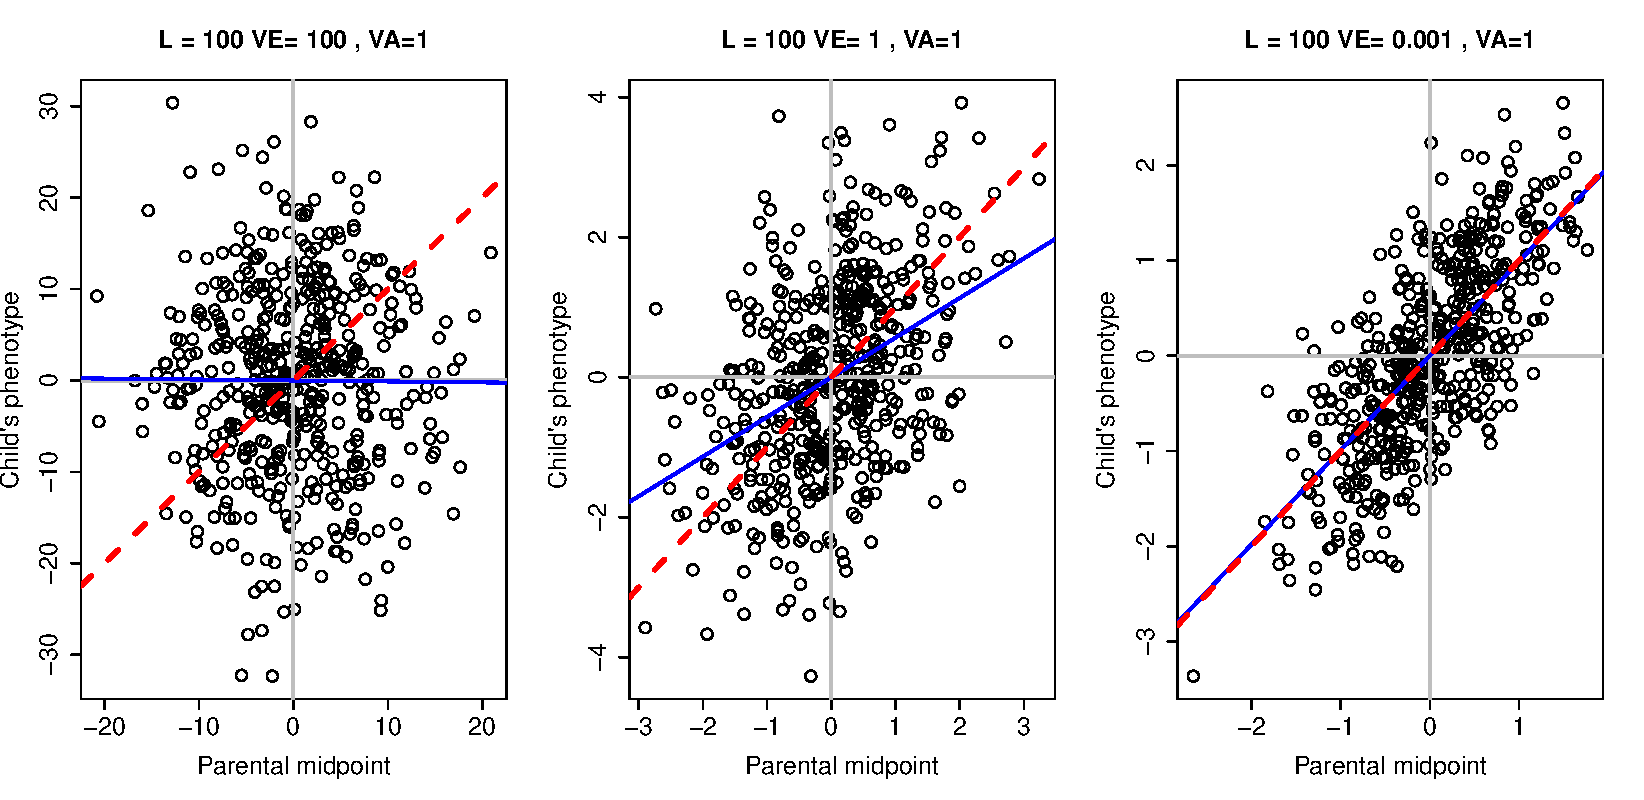
\includegraphics[width=\textwidth]{figures/QT2.pdf}
\end{center}
\caption{Regression of parental mid-point phenotype on child's
  phenotype. The three panels show decreasing levels of environmental
  variance ($V_E$) holding the additive genetic variance constant ($V_A=1$). 
 In these figures I simulate $100$ loci, as described in
 the caption of Figure \ref{fig:QT1}. I simulate the genotypes and
 phenotypes of the two parents, and then simulate the child's genotype
following mendelian transmission. The blue line shows $x=y$ the red
line shows the best fitting linear regression line. }
\end{figure}

More formally the expected phenotype of the child given the parental
phenotypes is
\begin{equation}
\E(X_{kid} | X_{mum},X_{dad}) = \mu +
\beta_{mid,kid}(X_{mid} - \mu) =\mu + h^2(X_{mid} - \mu)  \label{predict_kid}
\end{equation}
this follows from the definition of linear regression. So to find the
child's predicted phenotype we simply take the mean phenotype and add
on the difference between our parental mid-point multiplied by our
narrow sense heritability. \\


\begin{question}
Briefly explain Galton’s observation of the regression towards
mediocrity in light of Mendelian inheritance. 
\end{question}

\paragraph{Estimating additive genetic variance across a variety of
  different relationships.}

In many natural populations we may have access to individuals of a
range of different relationships to each other (through monitoring
of the paternity of individuals), but relatively few individuals of a
given relationship (e.g. sibs). We can try and use this information as
fully as possible in a mixed model framework. Considering equation
\ref{pheno_geno_environ} we can write an individual's phenotype $X_i$
 as 
\begin{equation}
X_i =  \mu  + X_{A,i} + e_i 
\end{equation}
where $e_i \sim N(0,V_E)$ and $X_{A,i}$ is normally distributed across
individuals with covariance matrix $V_A A$ where the the entries for
a pair of individuals i and j are 
$A_{ij}= 2 F_{i,j}$ and $A_{ii}= 1$. Given the matrix $A$ we can estimate $V_A$. We can
also add fixed effects into this model to account for generation
effects, additional mixed effects could also be included to account
for shared environments between particular individuals (e.g. a shared nest).
This is sometimes called the ``animal model'', and also goes by the
name of variance components analysis.


\subsection{The response to selection}
Evolution by natural selection requires:
\begin{enumerate}
\item Variation in a phenotype
\item That survival is non-random with respect to this phenotypic
variation.
\item That this variation is heritable.
\end{enumerate}
Points 1 and 2 encapsulate our idea of Natural Selection, but evolution by natural
selection will only occur if the 3rd condition is met. It is the
heritable nature of variation that couples change within a generation
due to natural selection, to change across generations (evolutionary
change). \\

Lets start by thinking about the change within a generation due
to directional selection, where selection acts to change the mean
phenotype within a generation. For example, a decrease in mean height within a
generation, due to taller organisms having a lower chance of surviving
to reproduction than shorter organisms. Specifically, we'll denote our mean phenotype at
reproduction by $\mu_S$, i.e. after selection has acted, and our mean
phenotype before selection acts by $\mu_{BS}$. This second quantity may be hard to
measure, as obviously selection acts throughout the life-cycle, so it
might be easier to think of this as the mean phenotype if selection
hadn't acted. So the mean phenotype changes within a generation is $\mu_{S} - \mu_{BS}= S$.  \\

We are interested in predicting the distribution of phenotypes in next
generation, in particular we are interested in the mean phenotype in
the next generation to understand how directional selection has
contributed to evolutionary change. We'll denote the mean phenotype in
offspring, i.e. the mean phenotype in the next generation before selection acts,
as $\mu_{NG}$. The change across generations we'll call the response
to selection $R$ and put this equal to $\mu_{NG}- \mu_{BS}$. \\

The mean phenotype in the next generation is
\begin{equation}
\mu_{NG} = \E \left( \E(X_{kid} | X_{mum},X_{dad}) \right)
\end{equation}
where the outer expectation is over the randomly mating of individuals
who survive to reproduce. We can use eqn. \ref{predict_kid} to obtain
an expression for this
\begin{equation}
\mu_{NG} = \mu_{BS} +
\beta_{mid,kid} ( \E(X_{mid}) - \mu_{BS})
\end{equation}
so to obtain $\mu_{NG}$ we need to compute $\E(X_{mid})$ the expected
mid-point phenotype of pairs of individuals who survive to
reproduce. Well this is just the expected phenotype in the individuals
who survived to reproduce ($\mu_{S}$), so
\begin{equation}
\mu_{NG} = \mu_{BS} +
h^2 (\mu_S - \mu_{BS})
\end{equation}
So we can write our response to selection as
\begin{equation}
R = \mu_{NG} -\mu_{BS}  =
h^2 (\mu_S - \mu_{BS}) = h^2 S \label{breeders_eqn}
\end{equation}
So our response to selection is proportional to our selection
differential, and the constant of proportionality is the narrow sense
heritability. This equation is sometimes termed the Breeders
equation. It is a statement that the evolutionary change across
generations ($R$) is proportional to the change caused by directional selection
within a generation, and the strength of this relationship is
determined by the narrow sense heritability. \\

Using the fact that $h^2=V_A/V$ we can rewrite this in a different form as
\begin{equation}
R= V_A \frac{S}{V}
\end{equation}
i.e. our response to selection is the additive genetic variance of our
trait ($V_A$) multiplied by the change within a generation as a
fraction of the total phenotypic variance ($S/V$, sometimes called the
the selection gradient $\beta$).\\

If our selection pressure is sustained over many generations we can
use our breeders equation to predict the response. If we are willing
to assume that our heritability does not change and we maintain a constant selection
gradient, then after $n$ generations our phenotype mean will have
shifted 
\begin{equation}
n h^2 S
\end{equation}
i.e. our population will keep up a linear response to selection.

\begin{figure}
\begin{center}
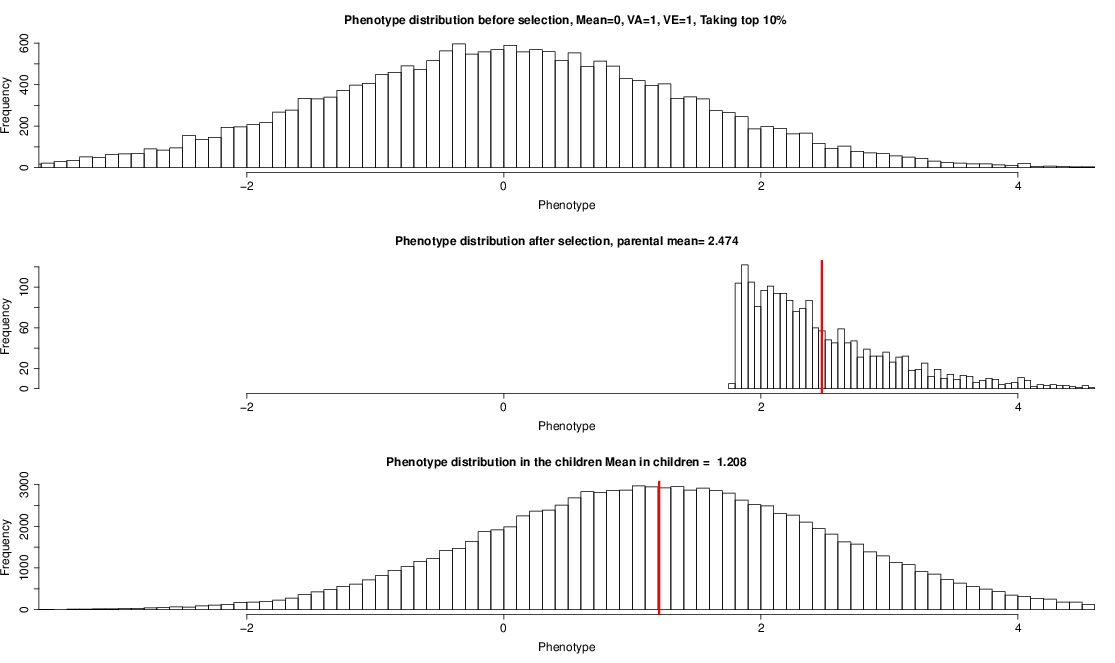
\includegraphics[width=0.8\textwidth]{figures/QT3.png}
\end{center}
\end{figure}

A change in mean phenotype within a generation occurs because of the
differential fitness of our organisms. To think more carefully about this change within a
generation lets think about a simple fitness model where our phenotype affects the
viability of our organisms (i.e. the probability they survive to
reproduce). The probability that an individual has a phenotype $X$
before selection is $p(X)$, so that the mean phenotype before
selection is
\begin{equation}
\mu_{BS} = \E[X] =  \int_{-\infty}^{\infty} x p(x) dx
\end{equation}
The probability that an organism with a phenotype $X$ survives to
reproduce is $w(X)$, and we'll think about this as the fitness of
our organism. The probability distribution of phenotypes in those who
do survive to reproduce is
\begin{equation}
\P(X | \textrm{survive}) =  \frac{p(x) w(x)}{
\int_{-\infty}^{\infty} p(x) w(x) dx}.
\end{equation}
where the denominator is a normalization constant which ensures that
our phenotypic distribution integrates to one. The denominator also
has the interpretation of being the mean fitness of the population,
which we'll call $\wbar$, i.e.  
\begin{equation}
\wbar =  
\int_{-\infty}^{\infty} p(x) w(x) dx.
\end{equation}

Therefore, we can write the mean phenotype in those who survive to
reproduce as
\begin{equation}
\mu_S = \frac{1}{\wbar}\int_{-\infty}^{\infty} x p(x) w(x) dx
\end{equation}

If we mean center our population, i.e. set the phenotype before
selection to zero, then
\begin{equation}
S= \frac{1}{\wbar}\int_{-\infty}^{\infty} x p(x) w(x) dx
\end{equation}
if $\mu_S=0$.  Inspecting this more closely we can see that $S$ has
the form of a covariance between our phenotype $X$ and our fitness
$w(X)$ ($Cov(X,w(X))$). Thus our change in mean phenotype is directly a measure of the
covariance of our phenotype and our fitness. Rewriting our breeder's
equation using this observation we see
\begin{equation}
R = \frac{V_A}{V}  Cov(X,w(X))
\end{equation}
we see that the response to selection is due to the fact that our
fitness (viability) of our organisms/parents covaries with our phenotype, and
that our child's phenotype is correlated with the parent phenotype.

\begin{question}
A student has been studying barnacle populations and has found the mean height (before selection) to be 10 mm and the variance in height to be 4 mm2.  After a stormy season (one generation), the mean of the population in the next generation before selection has increased to 12 mm.  In a breeding experiment, the student found the slope of the regression between parental midpoint and child to be 0.2.  Assuming the observed change was caused by selection, what was the mean height of the parents that survived the stormy season?  
\end{question}

\begin{question}
A population of red deer were trapped on Jersey (an island off of
England) during the last inter-glacial period. From the fossil record
we can see that the population rapidly adapted to their new
surroundings, presumably due to reduced predation and limited
food. Within 6,000 years they evolved from an estimated mean weight of
the population of 200kg to an estimated mean weight of 36kg (a 6 fold
reduction! True story see: \href{http://www.nature.com/nature/journal/v342/n6249/abs/342539a0.html}{Lister, A.M. Nature 1989}). Using a current
day population on the mainland you estimate that the generation time
of red deer is 5 years and that the narrow sense heritability of the
phenotype is 0.5. (Assuming discrete generations).\\
{\bf A)}	Estimate the mean change per generation in the mean body weight. \\

{\bf B)}	Estimate the change in mean body weight caused by selection within a generation.\\

{\bf C)}	What do you have to assume to perform the calculations in B. Assuming we only have fossils from the founding population and the population after 6000 years, should we assume that the calculations accurately reflect what actually occurred within our population?
\end{question}

\subsection{Multiple traits.}

Traits often covary with each other, due to both environmentally
induced effects (e.g. due to the effects of diet on multiple traits)
and due to the expression of underlying genetic covariance between
traits. In turn this genetic covariance can reflect pleiotropy, a
mechanistic effect of an allele on multiple traits (e.g. variants that
effect skin pigmentation often effect hair color) or the genetic
linkage of loci independently affecting multiple traits. If we are
interested in evolution over short time-scales we can (often) ignore
the genetic basis of this correlation. 

Consider two traits $X_{1,i}$ and $X_{2,i}$ in an indivdual $i$, these could be
say the individual's leg length and nose length. As before we can write
these as 
\begin{eqnarray}
X_{1,i} &= \mu_1+ X_{1,A,i} + X_{1,E,i}  \nonumber \\
X_{2,i} &= \mu_2 +X_{2,A,i} + X_{2,E,i} \nonumber \\
\end{eqnarray}
As before we can talk about the total phenotypic variance ($V_1,V_2$),
environmental variance  ($V_{1,E}$ and $V_{2,E}$), and the additive genetic variance in trait one and two
($V_{1,A}$, $V_{2,A}$). But now we also have to consider the 
total covariance $V_{1,2}=Cov(X_{1},X_{2})$, the environmentally induced covariance between the traits ($V_{E,1,2}=Cov(X_{1,E}
,X_{2,E} )$) and the additive genetic covariance ($V_{A,1,2}
=Cov(X_{1,A} ,X_{2,A} )$) between trait one and two.

We can store these values in a matrices 
\begin{equation}
\bf{V}= \left( \begin{array}{cc} 
V_{1} & V_{1,2} \\
V_{1,2} & V_{2} \\
\end{array} \right) \label{P_matrix}
\end{equation}
and
\begin{equation}
\bf{G}= \left( \begin{array}{cc} 
V_{1,A} & V_{A,1,2} \\
V_{A,1,2} & V_{2,A} \\
\end{array} \right)  \label{G_matrix}
\end{equation}
we can generalize this to an abitrary number of traits.

We can estimate these quantities, in a similar way to before, by
studying the covariance in different traits between relatives: 

\begin{equation}
Cov(X_{1,i},X_{2,j}) = 2 F_{i,j} V_{A,1,2}
\end{equation}

\paragraph{The response of multiple traits to selection, the
  multivariate breeder's equation.}
We can generalize these results for multiple traits, to ask how selection on
multiple phenotypes plays out over short time intervals. We'll write
our change in the mean our multiple phenotypes within a generation as
the vector $\bf{S}$ and our response across multiple generations as
the vector $\bf{R}$. These two quantities are related by 
\begin{equation}
\bf{R} = \bf{G} \bf{V}^{-1} \bf{S} = \bf{G} \bf{\beta}
\end{equation}
 where $\bf{V}$ and $\bf{G}$ are our matrices of the
 variance-covariance of phenotypes and additive genetic values
 (eqn. \eqref{G_matrix} \eqref{P_matrix}) and
 $\bf{\beta}$ is a vector of selection gradients (i.e. the change
 within a generation as a fraction of the total phenotypic variance).
To make this a bit more intuitive, consider two traits we are writing 
\begin{eqnarray}
R_1 & = V_{A,1} \beta_1 + V_{A,1,2} \beta_2 \nonumber \\
R_2 & = V_{A,2} \beta_2 + V_{A,1,2} \beta_1  \nonumber \\
\end{eqnarray}
where the $1$ and $2$ index our two different traits. This is a
statement that our response in any one phenotype is modified by
selection on other traits that covary with that trait.
This offers a good way to think about how genetic trade offs play out
over evolution over short time-scales.

\newpage
\subsection{Non-additive variation.}

Up to now we've assumed that our alleles contribute to our phenotype in an
additive fashion. However, that does not have to be the case as there may be
non-additivity among the alleles present at a locus (dominance) or among
alleles at different loci (epistasis). We can accommodate these complications
into our models. We do this by partitioning our total genetic variance into
independent variance components.

Consider autosomal biallelic locus $\ell$, with frequency $p$ for allele 1, and
genotypes $0$, $1$, and $2$ corresponding to how many copies of allele
1 individuals carry. We'll denote the mean phenotype of an individual
with genotype $0$, $1$, and $2$ are $\overline{X}_{\ell,0}$,
$\overline{X}_{\ell,1}$, $\overline{X}_{\ell,2}$ respectively. Here this mean is
taken over all the environments and genetic backgrounds the alleles
are present on. We'll mean center (MC)
these phenotypic values setting $\overline{X}'_{\ell,0} = \overline{X}_{\ell,0} - \mu$, and
likewise for the other genotypes. 

To illustrate the approach we'll plot two different cases of dominance
relationship in Figure \ref{fig:add_dom}. In the first row of Figure
\ref{fig:add_dom} we show the relationship between genotype and MC phenotype
under an additive model, and in the second row under a model where the allele 1
is dominant, such that the phenotype of the genotype of the heterozyote is the
same as the $11$ homozygote. The area of each circle is proportion to the
fraction of the population in each genotypic class ($p^2$, $2pq$, and $q^2$). 

\begin{figure}
\begin{center}
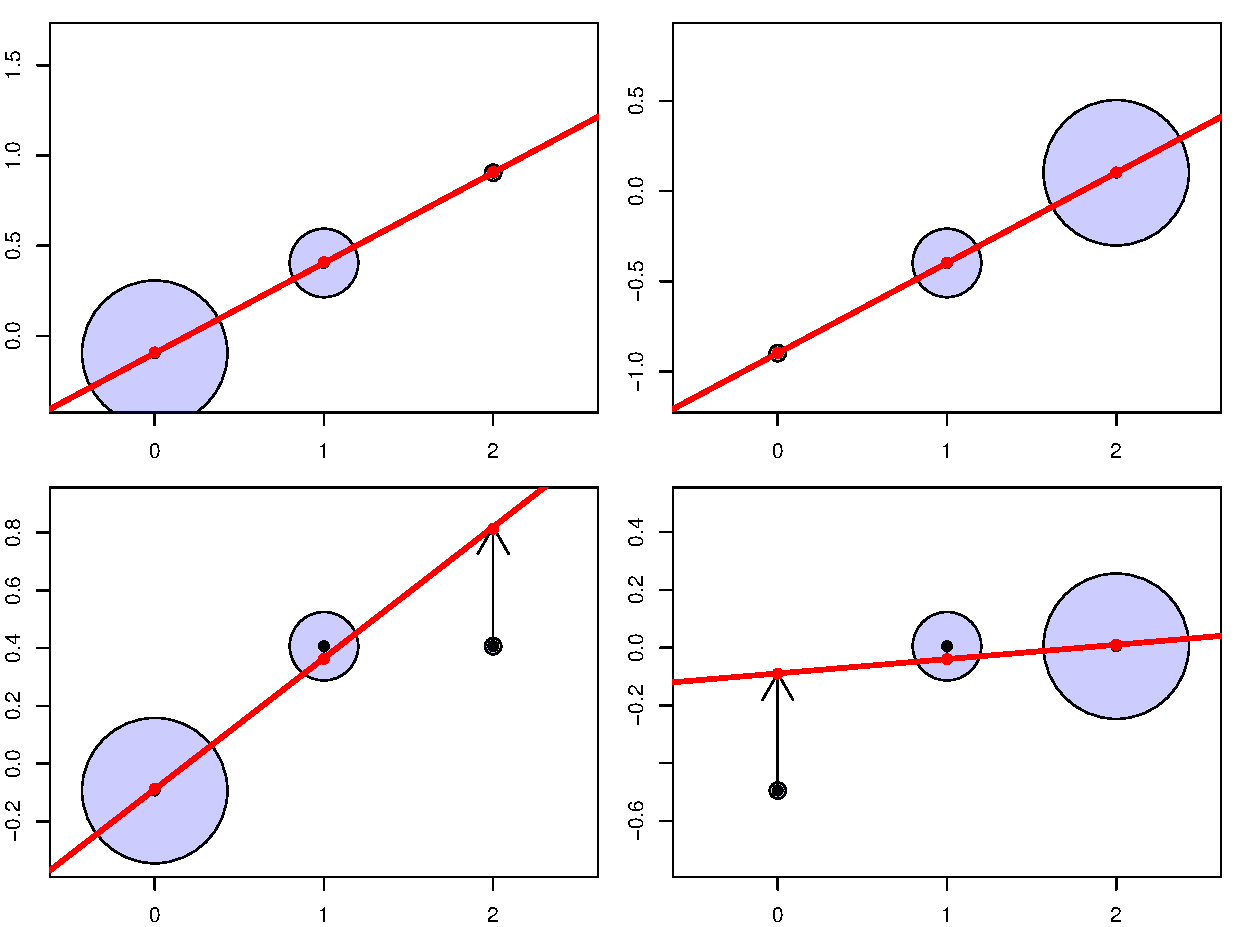
\includegraphics[width=\textwidth]{figures/additive_effect.pdf}
\end{center}
\caption{The average mean-centered (MC) phenotypes of each genotype. 
{\bf Top Row:} Additive relationship between genotype and phenotype. 
{\bf Bottom Row:} Allele 1 is dominant over allele 2, such that the
heterozygote has the same phenotype as the $22$ genotype ($2$). 
The area of each circle is proportion to the fraction of
the population in each genotypic class ($p^2$, $2pq$, and $q^2$). 
One the left column $p=0.1$ and the right column is $p=0.9$.
The additive genetic values of the genotypes are shown as
  red dots. The regression between phenotype and additive genotype is
  shown as a red line. The black vertical arrows show the difference
between the average MC phenotype and additive genetic value for each genotype. } \label{fig:add_dom}
\end{figure}

The first variance component is the variance due to
the additive contribution of each allele ($V_A$). 
We can think about the average
(marginal) MC
phenotype for an allele 1 as the average of the MC phenotype
for heterozgotes and 11 homozygotes weighted by the probability that
an allele $1$ in present in these genotypes. 
These marginal MC
phenotypes for allele 1 and 2 are given by 
\begin{equation} 
a_{\ell, 1} = p\overline{X}'_{\ell,2}  + q\overline{X}'_{\ell,1}, ~~ a_{\ell, 2} = p\overline{X}'_{\ell,1}  + q\overline{X}'_{\ell,0} 
\end{equation}
the marginal value for allele 1, $a_{\ell, 1}$,  follows from the fact that (assuming HW) an allele 1 will be
paired with another allele 1 with probability $p$, resulting in a
genotype $11$ (with phenotypic deviation $\overline{X}'_{\ell,2}$) and will
be paired with an allele 2 with probability $q$ in a heterozygote
(with phenotypic deviation $\overline{X}'_{\ell,1}$). A similar argument
can be made for $a_{\ell, 2}$. \\

The additive MC genetic values (breeding values) of genotype 0, 1, and
2 are then 
\begin{center}
\begin{tabular}{cccc}
genotype: & 0, & 1, & 2.\\
additive genetic value: & $a_{\ell,2}+ a_{\ell,2}$, & $a_{\ell,1}+a_{\ell,2}$, & $a_{\ell,1}+a_{\ell,1}$   \label{add_values}
\end{tabular}
\end{center}
%
Here we are simply adding up the additive contributions of the alleles present
in each genotype. These are the genotypic values of the trait that would result
taking only the additive component of the genotype.  They also have the
interpretation as being the mean phenotype of each genotypes' offspring
averaged over across all possible matings to other individuals in the
population (assuming individuals mate at random). 

The additive genetic values of the genotypes are shown as red dots in Figure
\ref{fig:add_dom}. Note that the additive values of the genotypes line up with
the observed MC phenotypic means in the top row when our alleles interact in a
completely additive manner. Our additive genetic values always fall along a
linear line (the red line in our figure). The additive values are falling best
fitting line of linear regression for our population, when phenotype is
regressed against the additive genotype ($0$, $1$, $2$ copies of allele 1)
across all individuals in our population. Note in the dominant case the
additive genetic values differ from the observed phenotypic means, and are
closer to the observed values for the genotypes that are common in the
population. \\

The difference in the additive effect of the two alleles $a_{\ell, 2}-a_{\ell,
1}$ can be interpreted as a average effect of swapping an allele 1 for an
allele 2, we'll call this difference $\alpha_{\ell}=a_{\ell, 2}-a_{\ell, 1}$.
Our $\alpha_{\ell}$ is also the slope of the regression of genotype against
phenotype (the red line in Figure \ref{fig:add_dom}). Note that the slope of
our regression of genotype on phenotype ($\alpha_{\ell}$) does not depend on
allele frequency for our completely additive locus (top row of
\ref{fig:add_dom}). In contrast, when there is dominance, our the slope between
genotype on phenotype ($\alpha_{\ell}$) is a function of allele frequency
(bottom row of \ref{fig:add_dom}). When a dominant allele (1) is rare there is
a strong slope of genotype on phenotype, bottom left Figure \ref{fig:add_dom}.
This strong slope is because replacing a single copy of the 2 allele with a 1
allele in an individual has a big effect on average phenotype, as it will most
likely move an individual from being a 22 homozygote to being a 12
heterozygote. However, when the dominant allele (1) is common in the
population, replacing a 2 allele by a 1 allele in an individual on average has
little phenotypic effect. This small effect is because as we are mainly turning
heterozygotes into homozygotes (11), who have the same mean phenotype.  \\

The variance in the population phenotype due to these
additive breeding values at locus $\ell$ assuming HW proportions is
\begin{align}
V_{A, \ell} &= p^2 (2a_{\ell,2})^2 + 2pq (a_{\ell,1}+a_{\ell,1})^2 + q^2
(2a_{\ell,0})^2 \nonumber \\
& = 2(p a_{\ell, 1}^2 + q a_{\ell, 2}^2 ) \nonumber \\
& = 2pq \alpha_{\ell}^2
\end{align}
The total additive effect can
be found by summing this additive genetic variance across loci
\begin{equation}
V_A = \sum_{\ell=1}^{L} V_{A, \ell} = \sum_{\ell=1}^{L}
2p_{\ell}q_{\ell} \alpha_{\ell}^2.
\end{equation}


Having assigned the additive genetic variance to be the variance
explained by the additive contribution of the alleles at a locus, we
define the dominance variance as the population variance among
genotypes at a locus due to their deviation from additivity.
We can calculate how much each genotypic mean deviates away from its
additive prediction at locus $\ell$ (the length of the arrows in
Figure \label{fig:add_dom}), for example the heterozygote deviates 
\begin{equation}
d_{\ell,1} =\overline{X}'_{\ell,1}  - (a_{\ell,1}+ a_{\ell,2})
\end{equation}
away from its additive genetic value, with similar expressions for
each of the homozygotes ($d_{\ell,0}$ and $d_{\ell,2}$). We can then write the dominance variance at
our locus as the genotype-frequency weighted sum of our squared
dominance deviations
\begin{equation}
V_{D,\ell} = p^2 d_{\ell,0}^2+ 2pq d_{\ell,1}^2+ q^2 d_{\ell,2}^2.
\end{equation}
Writing our total dominance variance as the sum across loci 
\begin{equation}
V_D = \sum_{\ell=1}^{L}  V_{D,\ell}. 
\end{equation}
Having now partitioned all of the genetic variance into additive and
dominant terms, we can write our total genetic variance as 
\begin{equation}
V_{G} = V_A+V_D.
\end{equation}
We can do this because by construction the covariance between our
additive and dominant deviations for the genotypes is zero. We can
define the narrow sense heritability as before
$h^2=V_A/V_P=V_A/(V_G+V_E)$, which is the proportion of phenotypic
variance due to additive genetic variance. We can also define the 
total proportion of the phenotype variance due to genetic differences
among individuals, as the broad-sense heritability $H^2 =
V_G/(V_G+V_E)$. \\

\begin{table}
\begin{center}
\begin{tabular}{| l | c|}
\hline
Relationship (i,j)$^{*}$ &  $Cov(X_i,X_j)$  \\
\hline
parent--child & $\nicefrac{1}{2} V_A$\\
full siblings &$\nicefrac{1}{2} V_A +\nicefrac{1}{4} V_D$\\
identical (monzygotic) twins & $V_A+V_D$ \\
$1^{st}$ cousins & $\nicefrac{1}{8} V_A$\\
\hline
\end{tabular}
\end{center}
\caption{Phenotypic covariance between some pairs of relatives,
  include the dominance variation. $^{*}$Assuming this is the only relationship
the pair of individuals share (above that expected from randomly
sampling individuals from the population). } % doesn't this implicitly assume an infinite population?
\label{table:domcovar}
\end{table}

When dominance is present in the loci influencing our trait ($V_D>0$), we need to modify our
phenotype covariance among relatives to account for this
non-additivity. Specifically our equation for the covariance among a
general pair of relatives
(eqn. \ref{additive_covar_general_rellys} for additive variation) becomes
\begin{equation}
 Cov(X_1,X_2) = 2 F_{1,2} V_A + r_2 V_D
\end{equation}
where $r_2$ is the probability that the pair of individuals share 2
alleles identical by descent, making the same assumptions (other than additivity) that we made in deriving
eqn. \ref{additive_covar_general_rellys}.  In table
\ref{table:domcovar} we show the phenotypic covariance for some common
pairs of relatives. The regression of offspring phenotype on parental
midpoint still has a slope $V_A/V_P$. 

Full sibs and parent-offspring have the same
covariance if there is no dominance variance (as they have the same
kinship coefficient $F_{1,2}$). However, when dominance
is present ($V_D>0$), full-sibs resemble each other more than
parent-offspring pairs. That's because parents and offspring share
precisely one allele, while full-sibs can share both alleles (i.e. the
full genotype at a locus) identical by descent. We can attempt to
estimate $V_D$ by comparing different sets of relationships. For
example non-identical twins (full sibs born at same time) 
should have $1/2$ the phenotypic covariance of identical twins if
$V_D=0$. Therefore, we can attempt to estimate $V_D$ by looking at
whether identical twins have more than twice the phenotypic covariance
than non-identical twins. \\

The most important aspect of this discussion for thinking about
evolutionary genetics is that the parent-offspring covariance is still
only a function of $V_A$. This is because our parent (e.g. the mother) transmits only a
single allele, at each locus, to its offspring. The other allele the
offspring receives is random (assuming random mating), as it comes
from the other unrelated parent (the father). Therefore, the average
effect on the offspring phenotype of
the allele the offspring receives from the mother, is averaged over
the random allele the child receives from the father. Thus we only
care about the additive effect of the allele, as parents transmit only
alleles not genotypes to their offspring. This means that the short-term response
to selection, as described by the breeder equation, depends only on
$V_A$ and the additive effect of alleles. Therefore, if we can
estimate the narrow-sense heritability we can predict the short-term response.
However, if alleles display dominance our value of $V_A$ will change
as our loci change frequency, e.g. as dominant alleles become common
in the population their contribution to $V_A$ decreases. Therefore,
our value of $V_A$ will not be a constant across generations.

Up to this point we have only considered
dominance and not epistasis. However, we include epistasis in a
similar manner (for example among pairs of loci). This gets a little
tricky to think about so we will only briefly explain it. 
 We can first estimate the additive effect of the
alleles by considering the effect of the alleles averaging over the
other alleles they are paired with, just as before. We can then
calculate the additive genetic variance from this. We can estimate
the dominance variance, by calculating the residual variance among
genotypes at a locus unexplained by the additive effect of the
loci. We can then estimate the epistatic variance by estimating the
residual variance left unexplained among the two locus genotypes from the additive and dominant
deviations calculated from each locus separately. In practice these
high variance components are hard to estimate, and usually small as
much of our variance is assigned to the additive effect.  Again we
would find that we mostly care about $V_A$ for predicting short-term
evolution, but that the contribution of loci to the additive genetic
variance will depend on the epstatic relationships among loci.


\begin{question}
You collect observations of red deer within a generation; recording an
individual’s number of offspring and phenotypes, which are known to
have additive genetic variation, and construct the plots shown in
Figure \ref{fig:red_deer_Q} (standardizing the phenotypes). Answer the following
questions. For each question choose one of the bold options. Briefly justify each of your answers with reference to the breeder's
equation and multi-trait breeder's equation. No calculations are required. \\
{\bf A)}	Looking at just at figure \ref{fig:red_deer_Q} A, in what direction do you expect male antler size to evolve? \\
{\bf Insufficient information, increase, decrease.}\\

{\bf B)}	Looking just at figures \ref{fig:red_deer_Q} B and C, in what direction do you expect male antler size to evolve? \\
{\bf Insufficient information, increase, decrease.}\\

{\bf C)}	(3 Points) Looking at figures \ref{fig:red_deer_Q} A, B, and C in what direction do you expect male antler size to evolve? \\
{\bf Insufficient information, increase, decrease.}\\
\end{question}

\begin{figure}
\begin{center}
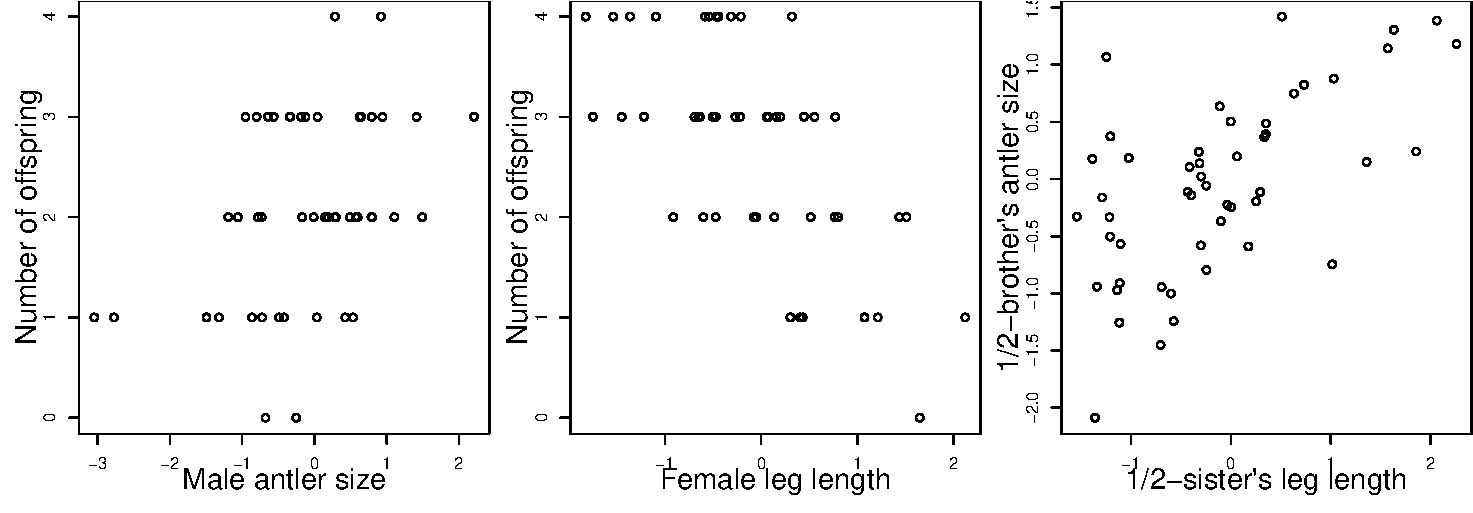
\includegraphics[width=\textwidth]{figures/Red_deer_selection.pdf}
\end{center}
\caption{ Observations of red deer within a generation; recording an
individual’s number of offspring and phenotypes, which are known to
have additive genetic variation. The figures left to right are A-C.} \label{fig:red_deer_Q}
\end{figure}



\begin{question}
How could you use 1/2 sibs vs full-sibs to estimate $V_D$? Why might
this be difficult in practice? Why are identical vs non-identical
twins better suited for this?
\end{question}

\begin{question}
Can you construct a case where $V_A=0$ and $V_D>0$? You need
just describe it qualitatively, you don't need to work out the
math. (tricker question).
\end{question}



\newpage

\chapter{One-locus models of selection}

\subsection{Fitness}

As we have seen, natural selection occurs when there are differences between individuals in fitness. We may define fitness in various ways. Most commonly, it is defined with respect to the contribution of a phenotype or genotype to the next generation. 
Differences in fitness can arise at any point during the life cycle. For instance, different genotypes or phenotypes may have different survival probabilities from one stage in their life to the stage of reproduction (viability), or they may differ in the number of offspring produced (fertility), or both. Here, we define the absolute fitness of a genotype as the expected number of offspring of an individual of that genotype. \\

\subsection{Haploid selection model}
We start out by modelling selection in a haploid model, as this is mathematically relatively simple. Let the number of individuals carrying alleles $A_1$ and $A_2$ in generation $t$ be $P_t$ and $Q_t$. Then, the relative frequencies at time $t$ of alleles $A_1$ and $A_2$ are $p_t = P_t / (P_t + Q_t)$ and $q_t = Q_t / (P_t + Q_t) = 1 - p_t$. Further, assume that individuals of type $A_1$ and $A_2$ on average produce $W_1$ and $W_2$ offspring individuals, respectively. We call $W_i$ the absolute fitness.\\

Therefore, in the next generation, the absolute number of carriers of $A_1$ and $A_2$ are $P_{t+1} = W_1 P_t$ and $Q_{t+1} = W_2 Q_t$, respectively. The mean absolute fitness of the population at time $t$ is
\begin{equation}
	\label{eq:meanAbsFit}
	\Wbar_t = W_1 \frac{P_t}{P_t + Q_t} + W_2 \frac{Q_t}{P_t + Q_t} = W_1 p_t + W_2 q_t,	
\end{equation}
i.e.\ the sum of the fitness of the two types weighted by their
relative frequencies. Note that the mean fitness depends on time, as
it is a function of the allele frequencies, which are themselves time
dependent. \\

The frequency of allele $A_1$ in the next generation is then given by
\begin{equation}
	\label{eq:eq:recHaplMod1}
	p_{t+1} = \frac{P_{t+1}}{P_{t+1} + Q_{t+1}} = \frac{W_1 P_t}{W_1 P_t + W_2 Q_t}
	%= \frac{W_1 (P_t + Q_t)p_t}{W_1 (P_t + Q_t)p_t + W_2 (P_t + Q_t)q_t}
	= \frac{W_1 p_t}{W_1 p_t + W_2 q_t} = \frac{W_1}{\Wbar_t} p_t.
\end{equation}


Importantly, eqn.\ (\ref{eq:eq:recHaplMod1}) tells us that the change in $p$ only depends on a ratio of fitnesses. Therefore, we need to specify fitness only up to an arbitrary constant. As long as we multiply all fitnesses by the same value, that constant will cancel out and eqn.\ (\ref{eq:eq:recHaplMod1}) will hold. Based on this argument, it is very common to scale absolute fitnesses by the absolute fitness of one of the genotypes, e.g.\ the most or the least fit genotype, to obtain relative fitnesses. Here, we will use $w_i$ for the relative fitness of genotype $i$. If we choose to scale by the absolute fitness of genotype $A_1$, we obtain the relative fitnesses $w_1 = W_1/W_1 = 1$ and $w_2 = W_2/W_1$.\\
Without loss of generality, we can therefore rewrite eqn.\ (\ref{eq:eq:recHaplMod1}) as
\begin{equation}
	\label{eq:recHaplMod2}
	p_{t+1} = \frac{w_1}{\wbar} p_t,
\end{equation}
dropping the dependence of the mean fitness on time in our notation, but remembering it.
The change in frequency from one generation to the next is then given by
\begin{equation}
\Delta p_t = p_{t+1} - p_t= \frac{ w_1 p_t}{ \wbar} - p_t = \frac{w_1 p_t - \wbar p_t}{\wbar} = \frac{w_1 p_t - (w_1 p_t + w_2 q_t) p_t}{\wbar} = \frac{w_1 - w_2}{\wbar} p_t q_t,
\label{eq:deltap_haploid}
\end{equation}
recalling that $q_t = 1 - p_t$.\\

Assuming that the fitnesses of the two alleles are constant over time,
the number of the two allelic types $\tau$ generations after time $t$ are
$P_{t+\tau} = (W_1)^{\tau} P_t$ and $Q_{t+\tau}=  (W_2)^{\tau} Q_t$, respectively. Therefore, the relative frequency of allele $A_1$ after $\tau$ generations past $t$ is
\begin{equation}
	p_{t+\tau} = \frac{ (W_1)^{\tau} P_t}{ (W_1)^{\tau} P_t+(W_2)^{\tau} Q_t} = \frac{ (w_1)^{\tau} P_t}{ (w_1)^{\tau} P_t+(w_2)^{\tau} Q_t} = \frac{p_t}{p_t + (w_2/w_1)^{\tau} q_t},
	\label{eq:haploid_tau_gen}
\end{equation}
where the last step includes dividing the whole term by $(w_1)^{\tau}$ and switching from absolute to relative allele frequencies.\\

Rearranging eqn.\ \eqref{eq:haploid_tau_gen} and setting $t = 0$, we can work out the time $\tau$ for the frequency of $A_1$ to change from $p_0$ to $p_{\tau}$. First, we write
\begin{equation}
	p_{\tau} = \frac{p_0}{p_0 + (w_2/w_1)^{\tau} q_0}
\end{equation}
and rearrange this to obtain
\begin{equation}
	\label{eq:estTau}
	\frac{p_{\tau}}{q_{\tau}} = \frac{p_0}{q_0} \left(\frac{w_1}{w_2}\right)^{\tau}.
\end{equation}
Solving this for $\tau$ yields
\begin{equation}
	\label{eq:solTau}
	\tau = \log \left(\frac{p_{\tau} q_0}{q_{\tau} p_0}\right) /  \log\left(  \frac{w_1}{w_2} \right).
\end{equation}
\\

In practice, it is often helpful to parametrize the relative fitnesses $w_i$ in a specific way. For example, we may set $w_1 = 1$ and $w_2 = 1 - s$, where $s$ is called the selection coefficient. Using this parametrization, $s$ is simply the difference in relative fitnesses between the two alleles. Equation \eqref{eq:haploid_tau_gen} becomes
\begin{equation}
	\label{eq:haploid_tau_gen_expl}
	p_{t+\tau} = \frac{p_{t}}{p_{t} + q_{t} (1 - s)^{\tau}},
\end{equation}
as $w_2 / w_1 = 1 - s$. Then, if $s \ll 1$, we can approximate $(1-s)^{\tau}$ in the denominator by $\exp(-s\tau)$ to obtain
\begin{equation} \label{eq:haploid_logistic growth}
	p_{t+\tau} \approx \frac{p_t}{p_t + q_t e^{-s\tau}}.
\end{equation}
This equation takes the form of a logistic function. That is because
we are looking at the relative frequencies of two `populations' (of
alleles $A_1$ and $A_2$) that are growing (or declining)
exponentially, under the constraint that $p$ and $q$ always sum to 1. \\

Moreover, eqn.\ \eqref{eq:estTau} for the time $\tau$ it takes for a certain change in frequency to occur becomes
\begin{equation}
	\label{eq:estTauExpl}
	\tau = - \log \left(\frac{p_{\tau} q_0}{q_{\tau} p_0}\right) /  \log\left(1-s\right).
\end{equation}
Assuming again that $s \ll 1$, this simplifies to
\begin{equation}
	\label{eq:estTauExplSimpl}
	\tau \approx \frac{1}{s} \log \left(\frac{p_{\tau} q_0}{q_{\tau} p_0}\right).
\end{equation}


One particular case of interest is the time it takes to go from an absolute
frequency of 1 to near fixation in a population of size $N$.  In this case, we
have $p_0 = 1/N$, and we may set $p_{\tau} = 1 - 1/N$, which is very close to
fixation. Then, plugging these values into eqn.\ \eqref{eq:estTauExplSimpl}, we
obtain

\begin{align}
  tau &= \frac{1}{s} \log\left( \frac{1 - \nicefrac{2}{N} +
      \nicefrac{1}{N^2}}{\nicefrac{1}{N^2}} \right) \nonumber \\
  &\approx \frac{1}{s} (\log(N) + \log(N-2)) \nonumber \\
  &\approx \frac{2}{s} \log(N)  \label{eq:fixTimeSimpl}
\end{align}
%
where we make the approximations $N^2 - 2N + 1 \approx N^2 - 2N$ and later
$N-2 \approx N$.

\begin{tcolorbox}
\begin{question}
You are studying the frequency of antibiotic-resistant bacteria in a
patient.  Before administering the antibiotic the frequency of the 
resistance allele is $\nicefrac{1}{1000}$. You adminster the antibiotic,
alarming just 8 days later you find the frequency of the 
resistance allele to be $99\%$. Assume a generation time of $\nicefrac{1}{4}$ a day for
these bacteria. \\
What is the selection coefficient associated with the resistance to antibiotics?
\end{question}
\end{tcolorbox}
\paragraph{Haploid model with fluctuating selection}
We can now consider the case where the fitnesses depend on time, and
say that $w_{1,t}$ and $w_{2,t}$ are the fitnesses of the two types in
generation $t$. The frequency of allele $A_1$ in generation $t+1$ is
\begin{equation}
p_{t+1} = \frac{w_{1,t}}{\wbar_t} p_t,
\end{equation}
which simply follows from eqn.\ \eqref{eq:recHaplMod2}.
The ratio of the frequency of allele $A_1$ to that of allele $A_2$ in generation $t+1$ is
\begin{equation}
\frac{p_{t+1}}{q_{t+1}} = \frac{w_{1,t}}{w_{2,t}}  \frac{p_{t}}{q_{t}}.
\end{equation}
Therefore, if we think of the two alleles starting in generation $t$ at
frequencies $p_t$ and $q_t$, then $\tau$ generations later,
\begin{equation}
\frac{p_{t+\tau}}{q_{t+\tau}} = \left(\prod_{i=t}^{\tau-1} \frac{w_{1,i}}{w_{2,i}}  \right) \frac{p_{t}}{q_{t}}.
\end{equation}
\\

The question of which allele is increasing or decreasing in frequency comes down
to whether $\left(\prod_{i=t}^{\tau-1} \frac{w_{1,i}}{w_{2,i}}  \right)$ is
$>1$ or $<1$. As it is a little hard to think about this ratio, we can
instead take the $\tau^{\mathrm{th}}$ root of it and consider
\begin{equation}
\sqrt[\tau]{\left(\prod_{i=t}^{\tau-1} \frac{w_{1,i}}{w_{2,i}}  \right)} = \frac{\sqrt[\tau]{\prod_{i=t}^{\tau-1}w_{1,i}}}{\sqrt[\tau]{\prod_{i=t}^{\tau-1}w_{2,i}}}.
\end{equation}
The term $\sqrt[\tau]{\prod_{i=t}^{\tau-1}w_{1,i}}$ is the geometric mean fitness of allele
 $A_1$ over the $\tau$ generations past generation $t$. Therefore, allele $A_1$ will only increase
in frequency if it has a higher geometric mean fitness than allele $A_2$
(at least in our simple deterministic model). \\


\subsection{Diploid model}
We will now move on to a diploid model of a single locus with two segregating alleles.
We will assume that the difference in fitness between the three
genotypes comes from differences in viability, i.e.\ differential
survival of individuals from the formation of zygotes to reproduction.  
We denote the absolute fitnesses of genotypes $A_1A_1$, $A_1A_2$, and $A_2A_2$ by $W_{11}$, $W_{12}$, and $W_{22}$. Specifically, $W_{ij}$ is the probability that a zygote of genotype $A_iA_j$ survives to reproduction.
Assuming that individuals mate at random, the number of zygotes that are of the three genotypes and form generation $t$ are
\begin{equation}
Np_t^2, ~~~  N2p_tq_t, ~~~ Nq_t^2.
\end{equation}

The mean fitness of the population of zygotes is then
\begin{equation}
	\Wbar_t = W_{11} p_t^2+W_{12} 2p_tq_t  +  W_{22} q_t^2.
\end{equation}
Again, this is simply the weighted mean of the genotypic fitnesses.
\\

How many zygotes of each of the three genotypes survive to reproduce?
An individual of genotype $A_1A_1$ has a probability of $W_{11}$ of
surviving to reproduce, and similarly for other genotypes. Therefore, the expected number of $A_1A_1$, $A_1A_2$, and $A_2A_2$ individuals who survive to reproduce is
\begin{equation}
	NW_{11} p_t^2, ~~~ NW_{12} 2p_tq_t , ~~~ N W_{22} q_t^2.
\end{equation}
It then follows that the total number of individuals who survive to
reproduce is
\begin{equation}
	N \left(W_{11} p_t^2+W_{12} 2p_tq_t  +  W_{22} q_t^2 \right).
\end{equation}
This is simply the mean fitness of the population multiplied by the
population size (i.e.\ $N \wbar$).\\

The relative frequency of $A_1A_1$ individuals at reproduction
is simply the number of $A_1A_1$ genotype individuals at reproduction ($NW_{11} p_t^2$)
divided by the total number of individuals who survive to reproduce
($N \Wbar$), and likewise for the other two genotypes.
Therefore, the relative frequency of individuals with the three different genotypes at reproduction is
\begin{equation}
	\frac{NW_{11} p_t^2}{N\Wbar}, ~~~ \frac{NW_{12} 2p_tq_t}{N\Wbar} , ~~~ \frac{N W_{22} q_t^2}{N\Wbar}
\end{equation}
(see Table \ref{dip_fitness_table}).\\

\begin{table}
\begin{center}
\begin{tabular}{lccc}
\hline
& $A_1A_1$ & $A_1A_2$ & $A_2A_2$\\
\hline
Absolute no. at birth & $Np_t^2$ & $N2p_tq_t$ & $Nq_t^2$\\
Fitnesses & $W_{11}$ & $W_{12}$& $W_{22}$\\
Absolute no.\ at reproduction & $NW_{11} p_t^2$ & $NW_{12} 2p_tq_t$& $N W_{22} q_t^2$\\
Relative freq.\ at reproduction & $\frac{NW_{11} p_t^2}{N \Wbar} = \frac{W_{11}}{\Wbar} p_{t}^2$ & $\frac{NW_{12} 2p_tq_t}{N
\Wbar} = \frac{W_{12}}{\Wbar} 2 p_{t} q_{t}$ & $\frac{N W_{22} q_t^2}{N\Wbar} = \frac{W_{22}}{\Wbar} q_{t}^2$\\
\end{tabular}
\end{center}
\caption{Relative genotype frequencies after one episode of viability selection.} \label{dip_fitness_table}
\end{table}

As there is no difference in the fecundity of the three genotypes, the
allele frequencies in the zygotes forming the next generation are simply the
allele frequency among the reproducing individuals of the previous generation. Hence, the frequency of $A_1$ in generation $t+1$ is
\begin{equation}
	p_{t+1} = \frac{W_{11} p_t^2 + W_{12} p_tq_t}{\Wbar}
	\label{pgen_dip}.
\end{equation}
Note that, again, the absolute value of the fitnesses is irrelevant to
the frequency of the allele. Therefore, we can just as easily replace
the absolute fitnesses with the relative fitnesses. That is, we may replace $W_{ij}$ by $w_{ij} = W_{ij}/W_{11}$, for instance. \\

\begin{tcolorbox} 
\begin{question}
You have been studying an annual wildflower for many generations with two color morphs orange and white. You have discovered that a single bi-allelic locus controls flower color, with the white allele being recessive. The pollinator of these plants is an almost blind bat, so individuals are pollinated at random with respect to flower color. Your population census of 200 individuals showed that the population consisted of 168 orange-flowered individuals, and 32 white-flowered individuals.\\
Heavy February rainfall creates optimal growing conditions for an
exotic herbivorous beetle with a preference for orange-flowered
individuals.  This year it arrives at your study site with a ravenous
appetite.  Only 50\% of orange-flowered individuals survive its wrath,
while 90\% of white-flowered individuals survive until the end of the
growing season.  \\
%Additionally, surviving orange flowered individuals produce 80 seeds on average, while surviving white-flowered individuals produce 100 seeds on average. 
{\bf A} What is the initial frequency of the white allele, and what do you
have to assume to obtain this?\\
{\bf B} What is the frequency of the white allele in the seeds forming the next generation?\\
\end{question}
\end{tcolorbox}

The change in frequency from generation $t$ to $t+1$ is
\begin{equation}
\Delta p_t = p_{t+1} -p_{t}= \frac{w_{11} p_t^2 + w_{12} p_tq_t}{\wbar} - p_t. \label{deltap_dip1}
\end{equation}
To simplify this equation, we will first define two variables $\wbar_1$ and $\wbar_2$ as
\begin{eqnarray}
	\wbar_1 & = w_{11} p_t + w_{12} q_t, \\
	\wbar_2 & =  w_{12} p_t+ w_{22} q_t.
\end{eqnarray}
These are called the marginal fitnesses of allele $A_1$
and $A_2$, respectively. They are so called as $\wbar_1$ is the
average fitness of an allele $A_1$, i.e.\ the fitness of $A_1$ in a
homozygote weighted by the probability it is in a homozygote ($p_t$)
plus the fitness of $A_1$ in a
heterozygote weighted by the probability it is in a heterozygote ($q_t$).
We further note that the mean relative fitness can be expressed in terms of the marginal fitnesses as
\begin{equation}
	\label{eq:meanFitInTermsOfMargFit}
	\wbar = \wbar_1 p_t + \wbar_2 q_t,
\end{equation}
where, for notational simplicity, we have omitted the dependence of mean and marginal fitnesses on time.\\

We can then rewrite eqn.\ \eqref{deltap_dip1} using $\wbar_1$ and $\wbar_2$ as
\begin{equation}
	\Delta p_t = \frac{ (\wbar_1-\wbar_2)}{\wbar} p_t q_t.
	\label{deltap_dip2}
\end{equation}
The sign of $\Delta p_t$, i.e. whether allele $A_1$ increases of decreases
in frequency, depends only on the sign of $(\wbar_1-\wbar_2)$.
The frequency of $A_1$ will keep increasing over the generations so
long as its marginal fitness is higher than that of $A_2$,
i.e.\ $\wbar_1 > \wbar_2$, while if $\wbar_1 < \wbar_2$, the
frequency of $A_1$ will decrease. Note the similarity between eqn.\ \eqref{deltap_dip2} and the respective expression for the haploid model in eqn.\ \eqref{eq:deltap_haploid}. (We will return to the
special case where $\wbar_1 = \wbar_2$ shortly).\\

We can also rewrite \eqref{deltap_dip1} as
\begin{equation}
\Delta p_t =\frac{1}{2} \frac{p_tq_t}{\wbar} \frac{d \wbar}{dp},
\label{deltap_dip3}
\end{equation}
the demonstration of this we leave to the reader.
This form shows that the frequency of $A_1$ will increase ($\Delta p_t > 0$) if the mean fitness is an increasing function of the frequency of $A_1$ (i.e.\ if $\frac{d \wbar}{dp}>0$). On the other hand, the frequency of $A_1$ will decrease ($\Delta p_t < 0$) if the mean fitness is a decreasing function of the frequency of $A_1$ (i.e.\ if $\frac{d \wbar}{dp}<0$).
%This form shows that
%$\Delta p_t$ in increase if $\frac{d \wbar}{dp}>1$, i.e. increasing the
%frequency of $1$ increases the mean fitness, while the frequency of
%the allele with decrease if this increases the mean fitness of the
%population ($\frac{d \wbar}{dp}>1$).
Thus, although selection acts on
individuals, under this simple model, selection is acting to increase
the mean fitness of the population. \sa{The rate of this increase is proportional to
the variance in allele frequencies within the population ($p_tq_t$).}\\
\begin{tcolorbox} 
\begin{question}
Show that eqns.\ \eqref{deltap_dip3} and \eqref{deltap_dip2} are
equivalent. (Trickier question.)\\
\end{question}
\end{tcolorbox}
So far, our treatment of the diploid model of selection has been in terms of generic fitnesses $w_{ij}$. In the following, we will use particular parametrizations to gain insight about two specific modes of selection: directional selection and heterozygote advantage.

%%Selection coeffs in diploid model
\subsection{Diploid directional selection}
Directional selection means that one of the two alleles always has higher marginal fitness than the other one. Let us assume that $A_1$ is the fitter allele, so that $w_{11} \geq w_{12} \geq w_{22}$, and hence $\wbar_1 > \wbar_2$\.
As we are interested in changes in allele frequencies, we \sa{may use} relative fitnesses. We parameterize the reduction in relative fitness in terms of a selection coefficient, similar to the
one we met in the haploid selection section, as follows:\\
\begin{center}
\begin{tabular}{lccc}
genotype & $A_1A_1$ & $A_1A_2$ & $A_2A_2$ \\
absolute fitness & $W_{11}$ & $ \geq W_{12} \geq$ & $W_{22}$ \\
relative fitness (generic) & $w_{11} = W_{11}/W_{11}$ & $w_{12} = W_{12}/W_{11}$ & $w_{22} = W_{22}/W_{11}$ \\
relative fitness  (specific) & $1$ & $1-sh$ & $1-s$. \\
\end{tabular}\\
\end{center}
Here, the selection coefficient $s$ is the difference in relative
fitness between the two homozygotes, and $h$ is the
dominance coefficient. \sa{For selection to be directional, we require that $0 \leq h \leq 1$ holds. The dominance coefficient allows us to move between two extremes. One is when $h = 0$, such that allele $A_1$ is fully dominant and $A_2$ fully recessive. In this case, the heterozygote $A_1A_2$ is as fit as the $A_1A_1$ homozgyote genotype. The inverse holds when $h = 1$, such that allele $A_1$ is fully recessive and $A_2$ fully dominant.}\\

%, of the $12$ and
%$22$ genotypes we will use selection coefficients $s_{12} \leq 0$ and
%$s_{22} \leq s_{12}$

We can then rewrite eqn.\ \eqref{deltap_dip2} as
\begin{equation}
\Delta p_t = \frac{p_ths + q_t s(1-h)}{\wbar}p_tq_t ,
\label{deltap_direct}
\end{equation}
where
\begin{equation}
\wbar_t = 1-2p_tq_t sh-q_t^2s.
\end{equation}\\

\begin{tcolorbox} 
\begin{question}
Comparing the red ($h=0$) and black ($h=0.5$) trajectories in Figure \ref{fig:diploid_traj}, provide an explanation for why $A_1$ increases faster initially if $h=0$, but then approaches fixation more slowly compared to the case of $h=0.5$.
\end{question}
\end{tcolorbox}

A special case is when $h = 0.5$. This case is the case of no dominance, as the interaction among alleles with respect to fitness is strictly additive. Then, eqn.\ \eqref{deltap_direct} simplifies to
\begin{equation}
	\Delta p_t = \frac{1}{2}\frac{s}{\wbar}p_tq_t .
	\label{deltap_add}
\end{equation}


If selection is very weak, i.e.\ $s \ll 1$, the denominator ($\wbar$) is close to $1$ and we have
\begin{equation}
	\Delta p_t = \frac{1}{2} s p_t q_t .
	\label{deltap_add_simpl}
\end{equation}
It is instructive to compare eqn.\ \eqref{deltap_add_simpl} to the respective expression under the haploid model. To this purpose, start from the generic term for $\Delta p_t$ under the haploid model in eqn.\ \eqref{eq:deltap_haploid} and set $w_1 = 1$ and $w_2 = 1-s$. Again, assume that $s$ is small, so that eqn.\ \eqref{eq:deltap_haploid} becomes $\Delta p_t = s p_t q_t$. Hence, if $s$ is small, the diploid model of directional selection without dominance is identical to the haploid model, up to a factor of $1/2$. That factor is due to the choice of the parametrisation; we could have set $w_{11} = 1$, $w_{12} = 1-s$, and $w_{22} = 1-2s$ in diploid model instead, in which case the agreement with the haploid model would be perfect.\\

From this analogy, we can borrow some insight we gained for the haploid model. Specifically, the trajectory of the frequency of allele $A_1$ in the diploid model without dominance follows a logistic growth curve similar to \eqref{eq:haploid_logistic growth}. Similarly, eqn.\ \ref{eq:fixTimeSimpl} for the haploid model suggests that in the diploid model without dominance it takes
\begin{equation}
	\tau \approx \frac{4}{s} \log(2N)  \label{eq:diploid_fix_time}
\end{equation}
generations for the favourable allele ($A_1$)
 to transit from its entry into the population ($p_0 =1/(2N)$)
to close to fixation ($p_{\tau} =1-1/(2N)$). Note again the difference
by a factor of 2 due to the choice of parametrization. Also, the total
number of alleles is $2N$ in the diploid model, rather than $N$, which
explains another factor of 2 in the argument of the logarithm. More
generally we can use this correspondance of the trajectory additive
diploid model to the haploid model to understand how quickly allele
frequencies should change given a selection coefficient between
arbitrary frequencies.\\

\begin{figure}
\begin{center}
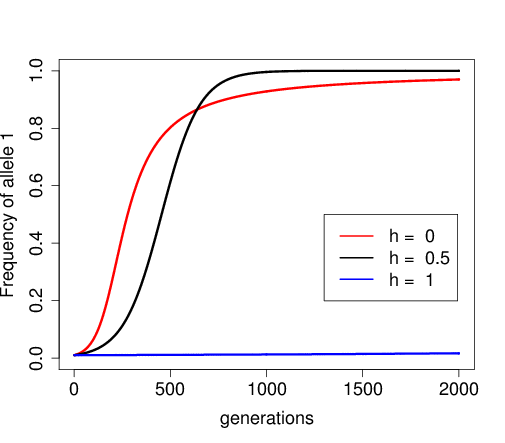
\includegraphics[width=0.5\textwidth]{figures/simple_diploid_trajs.png}
\end{center}
\caption{The trajectory of the frequency of allele $A_1$, starting
  from $p_{0}=0.01$, for a selection coefficient $s=0.01$ and three
  different dominance coefficients.}
  \label{fig:diploid_traj}
\end{figure}


%\begin{tcolorbox} 
%\begin{question}
%An autosomal pesticide resistance allele is at 50\% frequency in a species of flies.  We stop using the pesticide, and within 20 years the frequency of the allele is 5\% in the new-born flies. There are two fly generations per year. Assuming that the allele affects fitness in an additive fashion, estimate the selection coefficient acting against homozygotes for the resistance allele.
%\end{question}
%\end{tcolorbox}


\subsection{Heterozygote advantage}
What if the heterozygotes are fitter than either
of the homozygotes? In this case, it is useful to parameterize the relative fitnesses as follows:\\
\begin{center}
\begin{tabular}{lccc}
	genotype & $A_1A_1$ & $A_1A_2$ & $A_2A_2$ \\
	absolute fitness & $w_{11}$ & $<w_{12}>$ & $w_{22}$ \\
	relative fitness (generic) & $w_{11}=W_{11}/W_{12}$ & $w_{12} = W_{12}/W_{12}$ & $w_{22} = W_{22}/W_{12}$ \\
	relative fitness (specific)  & $1-s_1$ & $1$ & $1-s_2$ \\
\end{tabular}\\
\end{center}

Here, $s_1$ and $s_2$ are the differences between the relative fitnesses
of the two homozygotes and the heterozygote. Note that to obtain
relative fitnesses we have divided
absolute fitness by the heterozygote fitness. We could use the
same parameterization as in the model of directional selection, but the reparameterization we have chosen here makes the math prettier.\\

In this case, when allele $A_1$ is rare, it is often found in a
heterozygous state and so it increases in frequency. However, when
allele $A_1$ is common, it is often found in the homozygote state, while
the allele $A_2$ is often found in the heterozygote state; it is
now $A_2$ that increases in frequency at the expense of allele
$1$. Thus, at least in the deterministic model, neither allele can
reach fixation and both alleles will be maintained as a balanced
polymorphism in the population at an equilibrium frequency.\\

We can solve for this equilibrium frequency by setting $\Delta p_t = 0$ in  eqn.\ \eqref{deltap_dip2}, 
i.e.\ $p_tq_t (\wbar_1-\wbar_2)=0$. Doing so, we find that there are three equilibria, all of which are stable. Two of them are not very interesting ($p=0$ or $q=0$), but the third one is the polymorphic equilibrium,  where
$\wbar_1-\wbar_2$ holds.
Using the parametrization above, we see that the marginal fitnesses of the two alleles are formally equivalent. Insertion of the selection coefficients $s_1$ and $s_2$ yields
\begin{equation}
	p_e = \frac{s_2}{s_1+s_2}
\end{equation}
for the equilibrium frequency of interest. This is also the frequency of $A_1$ at which the mean fitness of the population is maximised.\\

\paragraph{Underdominance.} Another case that is of potential interest is the case of fitness
underdominance, where the heterozygote is less fit than either of the
homozygotes. This can be parametrized as follows: \\
\begin{center}
\begin{tabular}{lccc}
	genotype & $A_1A_1$ & $A_1A_2$ & $A_2A_2$ \\
	absolute fitness & $w_{11}$ & $<w_{12}>$ & $w_{22}$ \\
	relative fitness (generic) & $w_{11}=W_{11}/W_{12}$ & $w_{12} = W_{12}/W_{12}$ & $w_{22} = W_{22}/W_{12}$ \\
	relative fitness (specific)  & $1+s_1$ & $1$ & $1+s_2$ \\
\end{tabular}\\
\end{center}

This case also permits three equilibria, $p=0$, $p=1$, and a
polymorphic equilibrium $p=p_U$. However,
now only the first two equilibria are stable, while the polymorphic
equilibrium is unstable. If $p<p_U$ then $\Delta p_t $ is negative
and allele $A_1$ will be lost, while if $p>p_U$, allele
$A_1$ will become fixed.\\

While such alleles might not spread within populations (if $p_U \gg
0$ and selection is reasonably strong), they are of interest in the study of speciation and hybrid
zones. That is because alleles $A_1$ and $A_2$ may have arisen in a
stepwise fashion, i.e.\ not by a single mutation, in separate
subpopulations. Now, heterozygote disadvantage will play a
potential role in species maintenance, if isolation of the subpopulations is not complete.\\

\begin{tcolorbox} 
\begin{question}
You are studying the polymorphism that affects flight speed in butterflies. The polymorphism does not appear to affect fecundity.  Homozygotes for the B allele are slow in flight and so only 40\% of them survive to have offspring. Heterozygotes for the polymorphism (Bb) fly quickly and have a 70\% probability of surviving to reproduce. The homozygotes for the alternative allele (bb) fly very quickly indeed, but often die of exhaustion, with only 10\% of them making it to reproduction.  \\
{\bf A)} What is the equilibrium frequency of the B allele?\\
{\bf B)} Calculate the marginal fitnesses of the B and the b allele at
the equilbrium frequency. 
\end{question}
\end{tcolorbox}

\paragraph{Diploid fluctuating fitness}
We would like to think about the case where the diploid absolute fitnesses
are time-dependent. The three genotypes then have fitnesses
$w_{11,t}$, $w_{12,t}$, and $w_{22,t}$ in generation $t$. However,
this case is much less tractable than the haploid case, as segregation
makes it tricky to keep track of the genotype frequencies.  
We can make some progress and gain some intuition by thinking about
how the frequency of allele $A_1$ changes when it is rare.\\
% (This argument is originally due to Haldane and J. )\\

When $A_1$ is rare, i.e.\ $p_t \ll 1$, its frequency in the next
generation \eqref{pgen_dip} can be approximated as
\begin{equation}
p_{t+1} \approx \frac{w_{12}}{\wbar} p_t.
\end{equation}
To obtain this, we have ignored the $p_{t}^2$ term and assumed that $q_t \approx 1$ in the numerator.
Following a similar argument to approximate $q_{t+1}$, we can write
\begin{equation}
	\frac{p_{t+1}}{q_{t+1}} = \frac{w_{12,t}}{w_{22,t}}  \frac{p_{t}}{q_{t}}.
\end{equation}
Then, starting from out from $p_0$ and $q_0$ in generation $0$, $t+1$
generations later, we have
\begin{equation}
	\frac{p_{t+1}}{q_{t+1}} = \left( \prod_{i=0}^{t-1} \frac{w_{12,i}}{w_{22,i}}  \right) \frac{p_{0}}{q_{0}}.
\end{equation}
From this, we can see, following our haploid argument from above, that
the frequency of allele $A_1$ will increase when rare only if
\begin{equation}
	\frac{\sqrt[t]{\prod_{i=0}^{t-1}w_{12,i}}}{\sqrt[t]{\prod_{i=0}^{t-1}w_{22,i}}}>1 \label{geometric_1wins},
\end{equation}
i.e. if the heterozygote has higher geometric mean fitness than the $A_2A_2$ homozygote.\\

The question now is, whether allele $A_1$ will approach fixation in the population,
or whether there are cases in which we can obtain a balanced polymorphism. To investigate that, we can simply repeat our analysis for $q \ll 1$, and see that in that case
\begin{equation}
	\frac{p_{t+1}}{q_{t+1}} = \left( \prod_{i=0}^{t-1} \frac{w_{11,i}}{w_{12,i}}  \right) \frac{p_{0}}{q_{0}}.
\end{equation}
Now, for allele $A_1$ to carry on increasing in frequency and to
approach fixation, the $A_1A_1$ genotype has to be
out-competing the heterozygotes. For allele $A_1$ to approach
fixation, we need the geometric mean of $w_{11,i}$ to be greater than the
geometric mean fitness of heterozygotes ($w_{12,i}$).
At the same time, if heterozygotes have higher geometric mean fitness than
the $A_1A_1$ homozygotes, then the $A_2$ allele will increase in frequency when it is rare.
Therefore, a balanced polymorphism can result when the heterozygote
has higher geometric fitness than either of the homozygotes.\\

%\begin{equation}
%\frac{\sqrt[t]{\prod_{i=0}^{t}w_{11,i}}}{\sqrt[t]{\prod_{i=0}^{t}w_{22,i}}}>1
%\end{equation}
%implying that our $11$ homozygotes have to have higher geometric mean
%fitness than our heterozygotes.
%\begin{equation}
%\frac{\sqrt[t]{\prod_{i=0}^{t}w_{11,i}}}{\sqrt[t]{\prod_{i=0}^{t}w_{22,i}}}<1  \label{geometric_2wins}
%\end{equation}
%(satisfying both \eqref{geometric_1wins} and
%\eqref{geometric_2wins}).

Intriguingly, we can have a balanced polymorphism even if the
heterozygote is never the fittest genotype in any generation, if the heterozygotes
has a higher geometric mean fitness than either of the homozygotes. In this case, the polymorphism will remain balanced in the population,
despite the fact that the heterozygote is never the fitest genotype.

%To see
%this, consider the simple example, where there are two environments
%alternate from generation to generation:\\
%\begin{tabular}{lccc}
%genotype & $A_1A_1$ & $A_1A_2$ & $A_2A_2$ \\
%relative fitness in environment A & $w_{11,A}$ & $>w_{12,A}>$ & $w_{22,A}$ \\
%relative fitness in environment B  & $w_{11,B}$ & $<w_{12,B}<$ & $w_{22,B}$ \\
%Geometric mean fitness & $w_{11,B}$ & $<w_{12,B}>$ & $w_{22}$ \\
%\end{tabular}\\


\begin{tcolorbox}
\begin{question}
Consider a plant population found in one of two different environments each
generation. These occur randomly, $\nicefrac{1}{3}$ of time the population
experiences the dry environment and with probability $\nicefrac{2}{3}$ it
experiences the wet environment Y. The Absolute Fitnesses
are as follows:
\begin{center}
\begin{tabular}{cccc} 
Environment & AA & Aa & aa \\
\hline \\
Wet. & 6.25 & 5.0 & 3.75 \\
Dry & 3.85 & 5.0 & 6.15\\
\end{tabular}
\end{center}
{\bf A)} Show whether the equilibrium frequency of A will be $0$, $1$, or in between.\\
{\bf B)} If the probabilities of wet and dry environments were equal,
i.e., 0.5 how would your conclusion change?\\
(HINT: Lets write $w_{AA,\text{dry}}$ and $w_{AA,\text{wet}}$ for the
fitnesses of the AA homozygote in the two environments. Then if the
two environments are equally common $\prod_{i=0}^{t}w_{AA,i} \approx w_{AA,\text{dry}}^{\nicefrac{t}{2}}
w_{AA,\text{wet}}^{\nicefrac{t}{2}}$ for large values of $t$.)
%> (6.25)^(1/3)*(3.85)^(2/3);(5)^(1/3)*(5)^(2/3);(3.75)^(1/3)*(6.15)^(2/3)
%[1] 4.524812, 5, 5.215074
% (6.25)^(1/2)*(3.85)^(1/2);(5)^(1/2)*(5)^(1/2);(3.75)^(1/2)*(6.15)^(1/2)
% 4.905354, 5, 4.802343
\end{question}
\end{tcolorbox}

\begin{tcolorbox} 
\begin{question}
OPTIONAL trickier question.\\
Imagine a randomly-mating population of hermaphrodites. In this
population a derived allele (D) segregates that distorts transmission
in its favour over the ancestral allele (d) in the production of all
the gametes of heterozygotes. The drive leads to a fraction $r$ of the gametes
of heterozygotes (D/d) to carry the D allele ($r>0.5$). The D allele
causes viability problems in the homozygote state such that the
relative fitnesses are $w_{dd}=1$, $w_{Dd}=1$, $w_{DD}=1-e$. The allele
is currently at frequency p in the population at birth. Assuming that the
population is very large and no mutation occurs:\\
{\bf A)}	What is the frequency of the D allele in the next generation, before selection has had a chance to act?\\
{\bf B)}	What conditions do you need for a polymorphic equilibrium to be maintained? At what is the equilibrium frequency of this balanced polymorphism?\\
{\bf C)}	Imagine the cost of the driver were additive
$w_{dd}=1$, $w_{Dd}=1-e$, $w_{DD}=1-2e$. Under what conditions can the driver invade the population? Can a polymorphic equilibrium be maintained?
\end{question}
\end{tcolorbox}

\subsection{Mutation--selection balance}
%</source-file>
Mutation is constantly introducing new alleles into the
population. Therefore, variation can be maintained within a
population not only if selection is balancing (e.g.\ through heterozygote advantage or fluctuating selection over time, as we have seen in the previous section), but also due to a balance between
mutation and selection. A case of particular interest is when mutation introduces deleterious alleles and selection acts against these alleles. To study this balance, we return to the model of directional selection, where allele $A_1$ is advantageous, i.e.
\begin{center}
\begin{tabular}{lccc}
genotype & $A_1A_1$ & $A_1A_2$ & $A_2A_2$ \\
absolute fitness & $W_{11}$ & $ \geq W_{12} \geq$ & $W_{22}$ \\
relative fitness & $w_{11}=1$ & $w_{12}=1-sh$ & $w_{22}=1-s$. \\
\end{tabular}\\
\end{center}

For a start, we consider the case where allele $A_2$ is not
completely recessive ($h>0$), so that the heterozygotes suffer at least some disadvantage. We denote by $\mu = \mu_{1\rightarrow2}$ the  mutation rate per generation from $A_1$ to the deleterious allele $A_2$, and assume that there is no reverse mutation ($\mu_{2\rightarrow1} = 0$).  Let us assume that selection against $A_2$ is relatively strong compared to the mutation rate, so that it is justified to assume that $A_2$ is always rare, i.e.\ $q_t = 1-p_t \ll 1$. Compared to previous sections, for mathematical clarity, we also switch from following the frequency $p_t$ of $A_1$ to following the frequency $q_t$ of $A_2$. Of course, this is without loss of generality. The change in frequency of $A_2$ due to selection can be written as
\begin{equation}
	\Delta_S q_t = \frac{\wbar_2 - \wbar_1}{\wbar} p_t q_t  \approx  -hs q_t.
	\label{eq:dirSelApprox}
\end{equation}
This approximation can be found by assuming that $q^2 \approx 0$, $p \approx 1$,
and that $\wbar \approx w_1$. \sa{All of these assumptions make sense if $q \ll 1$. From eqn.\ \eqref{eq:dirSelApprox} we see that selection acts to reduce the frequency of $A_2$ (as both $h$ and $s$ are positive), and it does so geometrically across the
generations. That is, if the initial frequency of $A_2$ is $q_0$, then its frequency at time $t$ is approximately 
\begin{equation}
	q_t = q_0 (1 - hs)^t.
	\label{eq:dirSelExplApprox}
\end{equation}

We will now consider the change in frequency induced by mutation. Recalling that $\mu$ is
the mutation rate from $A_1$ to $A_2$ per generation, the frequency of $A_2$ after mutation
\begin{equation}
	q^{\prime} =  \mu p_t + q_t = \mu(1 - q_t) + q_t.
\end{equation}
Assuming that $\mu \ll 1$ and that $q \ll 1$, the change in the
frequency of allele $A_2$ due to mutation ($\Delta_M q_t$) can be approximated by
\begin{equation}
	\Delta_M q_t = q^{\prime} - q_t =  \mu.
	\label{eq:mutApprox}
\end{equation}
Hence, when $A_2$ is rare and the mutation rate is low, mutation acts to linearly increase the frequency of the deleterious allele $A_2$.\\

If selection is to balance deleterious mutation, their combined effect over one generation has to be zero. Therefore, to find the mutation--selection equilibrium, we set
\begin{equation}
	\Delta_M q_t + \Delta_S q_t = 0,
\end{equation}
insert eqns. \eqref{eq:dirSelApprox} and \eqref{eq:mutApprox}, and solve for $q$ to obtain
\begin{equation}
	q_e = q_t = \frac{\mu}{hs}.
	\label{eqn:mut_sel_bal}
\end{equation}
We see that the frequency of the deleterious allele $A_2$ is balanced at the mutation rate ($\mu$) divided by
the reduction in relative fitness in the heterozygote ($hs$).}\\

It is worth pointing out that the fitness of the $A_2A_2$ homozygote
has not entered this calculation, as $A_2$ is so rare that it is hardly ever found in the 
homozygous state. Therefore, if $A_2$ has any deleterious effect
in a heterozygous state (i.e.\ if $h>0$) it is this effect that determines the
frequency at which $A_2$ is maintained in the population. Also, note that by
writing the total change in allele frequency as $\Delta_M q_t + \Delta_S q_t
$ we have implicitly assumed that we can ignore terms of order $\mu
\times s$. That is, we have assumed that there is no interaction between mutation and selection. We can do so as we assumed that both $\mu$ and $s$ are small.\\


What effect do such deleterious mutations at mutation--selection balance have on the population? It is common to express this effect in terms of a reduction of the mean relative fitness of the population. For a single site at which a deleterious mutation is segregating at $q_e = \mu/(hs)$, the mean relative fitness is reduced to
\begin{equation}
	\wbar = 1- 2p_e q_e hs - q_e^2s \approx 1-2\mu.
\end{equation}
Somewhat remarkably, the drop in mean fitness due to a site segregating
at mutation--selection balance is independent of the selection coefficient against the
heterozygote; it depends only the mutation rate. Note that this applies only if the mutation is not totally recessive, i.e.\ if $h > 0$.

A reduction of $1 - 2\mu$ is very small, given that the
mutation rate of a gene is likely $<10^{-5}$. However, if there are many loci
segregating at mutation--selection balance, this can accumulate to a substantial so-called
genetic load, and a major cause of variation in fitness-related traits among individuals.

As an aside, if an allele was truly recessive (although few likely are), we have $h=0$, and
so eqn.\ \eqref{eqn:mut_sel_bal} is not valid. However, we can make an argument similar to the one above to show
that, for truly recessive alleles,
\begin{equation}
	q_e = \sqrt{\frac{\mu}{s}}.
\end{equation}


\begin{tcolorbox} 
\begin{question}
You are studying an outbred population of mice living in a farmer’s field. Mutations occur at a gene called nurseryrhyme that cause a totally recessive form of blindness. These blind mice do not survive to reproduce as the farmer’s wife cuts off their tail (and other bits) with a carving knife. 
Surveying the field for baby mice you find that 3 in ten thousand mice are blind.\\
{\bf A} Assuming that the population mates at random, what is the mutation
 rate of blindness causing alleles?\\
{\bf B} Following more careful study you now find that there is actually a $20
\%$ reduction in the viability of heterozygotes for these
mutations. What would you now estimate as the mutation rate for this
gene?  
{\bf C)} Explain how and why your answers differ?
\end{question}
\end{tcolorbox}

%B) You look at family of outbred mice. You find that one of the mice in the family is blind, what is the probability that its 1st cousin is also blind?

%C) In another isolated field on the farm, there is a high rate of inbreeding among the mice. The farmer’s wife also carries out her cruel carving knife policy in this field as well. Do you expect to the underlying blindness mutations to be at a higher or low rate in this second field than the first field? Briefly explain your answer.


\subsection{Inbreeding depression}
All else being equal, eqn.\ \eqref{eqn:mut_sel_bal} suggests that mutations that have a smaller effect in the
heterozygote can segregate at higher frequency under mutation--selection balance. As a consequence, alleles that have
strongly deleterious effects in the homozygous state can segregate at
low frequencies in the population, as long as they do not have a
strong effect in heterozygotes. Thus, outbred populations may have many
alleles with recessive deleterious effects segregating within them.

One consequence of this is that inbred individuals from usually outbred
populations may have dramatically lower fitnesses than outbred
individuals. This is a consequence of being homozygous at many loci for
alleles with recessive deleterious effects. Indeed, this seems to be a common observation, dating back to systematic surveys by
Darwin. In typically outbred populations, the mean fitness of individuals
decreases with the inbreeding coefficient, i.e.\ this so-called inbreeding depression
is a common observation.

\paragraph{Purging the inbreeding load.}
Populations that regularly inbreed over sustained periods of time
are expected to partially purge this load of deleterious
alleles. This is because such populations have exposed many of these alleles
in a homozygous state, and so selection can more readily remove these alleles
from the population.

\newpage
\subsection{Migration--selection balance}
Another reason for the persistence of deleterious alleles in a
population is that there is a constant influx of maladaptive alleles
from other populations where these alleles are locally adapted.
This seems unlikely to be as broad an explanation for the
persistence of deleterious alleles genome-wide as mutation-selection
balance. However, a brief discussion of such alleles is worthwhile as
it helps to inform our ideas about local adaptation.\\

As a first pass at this lets consider a haploid two allele model with
two different populations, where the relative fitnesses of our alleles
are as follows
\begin{center}
\begin{tabular}{c|cc}
allele & $1$ & $2$ \\
\hline
population 1 & 1 & 1-s \\
population 2 & 1-s & 1 \\
\end{tabular}
\end{center}
As a simple model of migration lets suppose within a population a
fraction of $m$ individuals are migrants from the other population,
and $1-m$ individuals are from the same deme.\\

To quickly sketch a solution to this, we'll set up a situation analogous
to our mutation-selection balance model. To do this let's assume that selection is strong compared to migration ($s \gg m$) then allele
$1$ will be almost fixed in population $1$ and allele $2$ will be
almost fixed in population $2$. If that is the case,
migration changes the frequency of allele $2$ in population $1$ ($q_1$) by
\begin{equation}
\Delta_{Mig.} q_1 \approx m
\end{equation}
while as noted above $\Delta_{S} q_1= -sq_1$, so that migration and
selection are at an equilibrium when $0 = \Delta_{S} q_1+
\Delta_{Mig.}q_1$, i.e. an equilibrium frequency of allele $2$ in
population $1$ of
\begin{equation}
q_{e,1} = \frac{m}{s}
\end{equation}
so that migration is playing the role of mutation and so
migration-selection balance (at least under strong selection) is
analogous to mutation selection balance.\\

We can use this same model by analogy for the case of
migration-selection balance in a diploid model, in that case we replace
our haploid $s$ by the cost to heterozygotes $hs$.

\begin{tcolorbox} 
\begin{question}
You are investigating a small river population of sticklebacks, which receives infrequent migrants from a very large marine population. At a set of (putatively) neutral biallelic markers the freshwater population has frequencies:\\
0.2, 0.7, 0.8\\
at the same markers the marine population has frequencies:\\
0.4, 0.5 and 0.7.\\
 From studying patterns of heterozygosity at a large collection of markers, you have estimated the long term effective size of your freshwater population is 2000 individuals.\\
{\bf A)}	What is $F_{ST}$ across these neutral markers in the freshwater population, with respect to the large marine population (i.e. treat the marine population as the total)?\\
{\bf B)} You are also studying an unlinked locus involved in the
regulation of salt uptake. In the marine population the ancestral
allele is at close to fixation, but in your river population the
derived allele is at 0.99 frequency. Estimate the selective
disadvantage of the ancestral allele in your river population. [Hint
how can you use neutral differentiation to estimate the migration rate?]
\end{question}
\end{tcolorbox}
 
\subsection{Some theory of the spatial distribution of allele
frequencies under deterministic models of selection}

Imagine a continuous haploid population spread out along a line. Individuals
disperse a random distance $\Delta x$ from its birthplace to the location where
it reproduces, where $\Delta x$ is drawn from the probability density $g(~)$.
To make life simple we will assume that $g(\Delta x)$ is normally distributed
with mean zero and standard deviation $\sigma$, i.e. migration is unbiased an
individuals migrate an average distance of $\sigma$. \\

Our frequency of allele $2$ at time $t$ in the population at spatial location
$x$ is $q(x,t)$. Assuming that only dispersal occurs, how does our allele
frequency change in the next generation? Our allele frequency in the next
generation at location $x$ reflects the migration from different locations in
the proceeding generation. Our population at location $x$ receives a
contribution $g(\Delta x)q(x+\Delta x,t)$ of allele $2$ from the population at
location $x+\Delta x$, such that the frequency of our allele at $x$ in the next
generation is \begin{equation} q(x,t+1) = \int_{-\infty}^{\infty} g(\Delta
x)q(x+\Delta x,t) d \Delta x.  \end{equation}

To obtain $q(x+\Delta x,t)$, lets take a Taylor series expansion of $q(x, t)$

\begin{equation}
q(x+\Delta x,t) = q(x,t) + \Delta x \frac{dq(x,t)}{dx}+ \tfrac{1}{2}(\Delta x)^2 \frac{d^2q(x,t)}{dx^2}+\cdots
\end{equation}

then

\begin{equation}
q(x,t+1) = q(x,t) +\left( \int_{-\infty}^{\infty} \Delta x g(\Delta x) 
  d \Delta x \right) \frac{dq(x,t)}{dx} + \tfrac{1}{2}\left( \int_{-\infty}^{\infty}(\Delta x)^2 g(\Delta x) 
  d \Delta x \right)  \frac{d^2q(x,t)}{dx^2}+\cdots
\end{equation} 

$g(~)$ has a mean of zero so $ \int_{-\infty}^{\infty} \Delta x g(\Delta x) d
\Delta x =0$ and has variance $\sigma^2$ so $\int_{-\infty}^{\infty}(\Delta
x)^2 g(\Delta x) d \Delta x = \sigma^2$ and all higher terms are zero (as all
high moments of the normal are zero). Looking at the change in frequency
$\Delta q(x,t) = q(x,t+1)-q(x,t)$ then 

\begin{equation}
\Delta q(x,t) = \frac{\sigma^2}{2} \frac{d^2q(x,t)}{dx^2}
\end{equation} 

This is a diffusion equation, so that migration is acting to smooth
out allele frequency differences with a diffusion constant
of $\tfrac{\sigma^2}{2}$. This is exactly analogous to the equation
describing how a gas diffuses out to equal density, as both particles
in a gas and our individuals of type $2$ are performing Brownian
motion (blurring our eyes and seeing time as continuous). \\


We will now introduce fitness differences into our model and set the relative
fitnesses of allele $1$ and $2$ at location $x $ to be $1$ and $1+s\gamma(x)$.
To make progress in this model we'll have to assume that selection isn't too
strong i.e. $ s \gamma(x) \ll 1$ for all $x$. The change in
frequency of allele $2$ obtained within a generation due to selection is

\begin{equation}
q^{\prime}(x,t) - q(x,t) \approx s\gamma(x) q(x,t) \big( 1 - q(x,t) \big)
\end{equation}

i.e. logistic growth of our favoured allele at location $x$.  Putting our
selection and migration terms together we find \begin{equation} q(x,t+1) -
q(x,t) = s\gamma(x) q(x,t) \big( 1 - q(x,t) \big)+\frac{\sigma^2}{2}
\frac{d^2q(x,t)}{dx^2} \label{eqn:fisherKPP} \end{equation} in deriving this we
have essentially assumed that migration acted upon our original frequencies
before selection and in doing so have ignored terms of the order of $\sigma s$. 


\begin{figure}
\begin{center}
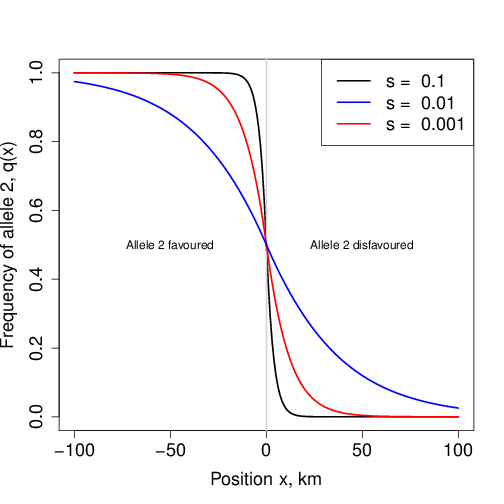
\includegraphics[width=0.5\textwidth]{figures/equilib_cline.png}
\end{center}
\caption{An equilibrium cline in allele frequency. Our individuals
  dispersal an average distance of $\sigma=1$km per generation, and our
allele $2$ has a relative fitness of $1+s$ and $1-s$ on either side of
the environmental change at $x=0$.} \label{fig:cline}
\end{figure}

\paragraph{The cline in allele frequency associated with a sharp
  environmental transition.}
To make progress lets consider a simple model of location adaptation where the
environment abruptly changes. Specifically we assume that $\gamma(x)= 1$ for
$x<0$ and $\gamma(x)= -1$ for $x \geq 0$, i.e. our allele $2$ has a selective
advantage at locations to the left of zero, while this allele is at a
disadvantage to the right of zero. In this case we can get an equilibrium
distribution of our two alleles were to the left of $zero$ our allele $2$ is at
higher frequency, while to the right of zero allele $1$ predominates. As we
cross from the left to the right side of our range the frequency of our allele
$2$ decreases in a smooth cline.\\



%Under such a model the change in frequency of allele $2$ at location $x$ at time $t$,
%$q(x,t)$, over time follows the differential equation
%\begin{equation}
%\frac{dq(x,t)}{dt} = s\gamma(x) q(x,t) \left( 1 - q(x,t) \right) + \frac{\sigma^2}{2} \frac{d^2q(x,t)}{dx^2}
%\end{equation}
%the first term on the right-hand side is the logistic growth of our
%favoured allele at location $x$, while the second term on the
%right-hand side is the diffusion of allele frequencies due to
%dispersal (i.e. dispersal is acting to spread out the effect of
%allele frequency change across populations). See below for how we
%derive this \gc{to be added}.\\

Our equilibrium spatial distribution of allele frequencies can be found by
setting the LHS of eqn. \eqref{eqn:fisherKPP} to zero to arrive at
\begin{equation}
s\gamma(x) q(x) \left( 1 - q(x) \right) = - \frac{\sigma^2}{2} \frac{d^2q(x)}{dx^2}
\end{equation}
We then could solve this differential equation with appropriate boundary
conditions ($q(-\infty)=1$ and $q(\infty) = 0$) to arrive at the
appropriate functional form to our cline. While we won't go into the
solution of this equation here, we can note that by dividing our
distance $x$ by $\ell=\sigma/\sqrt{s}$ we can remove the effect of our
parameters from the above equation. This compound parameter $\ell$ is the characteristic
length of our cline, and it is this parameter which determines over
what geographic scale we change from allele $2$ predominating to
allele $1$ predominating as we move across our environmental shift. \\

The width of our cline, i.e. over what distance do we make this shift
from allele $2$ predominating to allele $1$,
can be defined in a number of different ways. One simple way to define
the cline width, which is easy to define but perhaps hard to measure accurately, is the slope (i.e. the
tangent) of $q(x)$ at $x=0$. Under this definition the cline width is approximately $0.6
\sigma/\sqrt{s}$.\\

\paragraph{The rate of spatial spread of a beneficial allele.}
Consider a beneficial mutation that has arisen in a specific spatial
location and has begun to spread geographically. 
\gc{FINISH THIS.}


\newpage

\section{Stochasticity and Genetic Drift in allele frequencies}
\subsection{Stochastic loss of strongly selected alleles}
% Fisher (1922, 1930) and Haldane (1927)
Even strongly selected alleles can be lost from the population when
they are sufficiently rare. This is because the number of offspring
left by individuals to the next generation is fundamentally
stochastic. A selection coefficient of s=$1\%$ is a strong
selection coefficient, which can drive an allele through the
population in a few hundred generations once the allele is
established. However, if individuals have on average a small number of
offspring per generation the first individual to carry our allele who
has on average $1\%$ more children could easily have zero offspring, leading to the loss
of our allele before it ever get a chance to spread.\\

To take a first stab at this problem lets think of a very large
haploid population, and in order for this population to stay constant in size
we'll assume that individuals without the selected mutation have on average one
offspring per generation. While individuals with our selected allele
have on average $1+s$ offspring per generation. We'll assume that the
distribution of offspring number of an individual is Poisson
distributed with this mean, i.e. the probability that an individual
with the selected allele has $i$ children is
\begin{equation}
P_i= \frac{(1+s)^i e^{-(1+s)}}{i!}
\end{equation}


Consider starting from a single individual with the selected allele, and ask
about the probability of eventual loss of our selected allele starting
from this single copy ($p_L$). To derive this we'll make use of a
simple argument (derived from branching processes). Our selected
allele will be eventually lost from the population if every individual
with the allele fails to leave descendants.
\begin{enumerate}
\item In our first generation
with probability $P_0$ our individual leaves no copies of itself to
the next generation, in which case our allele is lost (Figure \ref{fig:Proof_of_pL_2s}A).
\item Alternatively
it could leave one copy of itself to the next generation (with
probability $P_1$), in which
case with probability $p_L$ this copy eventually goes extinct (Figure \ref{fig:Proof_of_pL_2s}B).
\item It could leave two copies of itself to the next generation (with
probability $P_2$), in which
case with probability $p_L^2$ both of these copies eventually goes
extinct (Figure \ref{fig:Proof_of_pL_2s}C).
\item More generally it could leave could leave $k$ copies ($k>0$) of itself to the next generation (with
probability $P_k$), in which case with probability $p_L^k$  all of
these copies eventually go extinct (e.g. Figure \ref{fig:Proof_of_pL_2s}D).
\end{enumerate}
summing over these probabilities we see that
\begin{eqnarray}
p_L &= \sum_{k=0}^{\infty} P_k p_L^{k}  \nonumber \\
&=  \sum_{k=0}^{\infty} \frac{(1+s)^ke^{-(1+s)}}{k!} p_L^{k} \nonumber
\\
&= e^{-(1+s)} \left( \sum_{k=0}^{\infty} \frac{\left(p_L(1+s) \right)^k}{k!}  \right)
\end{eqnarray}
well the term in the brackets is itself an exponential expansion, so
we can rewrite this as
\begin{equation}
p_L = e^{(1+s)(p_L-1)} \label{prob_loss}
\end{equation}
solving this would give us our probability of loss for any selection
coefficient. Lets
rewrite this in terms of the the probability of escaping loss $p_F = 1-p_L$.  We can
rewrite eqn \eqref{prob_loss} as
\begin{equation}
1-p_F = e^{-p_F(1+s)}
\end{equation}
to gain an approximation to this lets consider a small selection
coefficient $s \ll 1$ such that $p_F \ll 1$ and then expanded out the
exponential on the right hand side (ignoring terms of higher
order than $s^2$ and $p_F^2$) then
\begin{equation}
1-p_F \approx 1-p_F(1+s)+p_F^2(1+s)^2/2
\end{equation}
solving this we find that
\begin{equation}
p_F = 2s.
\end{equation}
Thus even an allele with a $1\%$ selection coefficient has a $98\%$
probability of being lost when it is first introduced into the
population by mutation.\\

\begin{figure}
\begin{center}
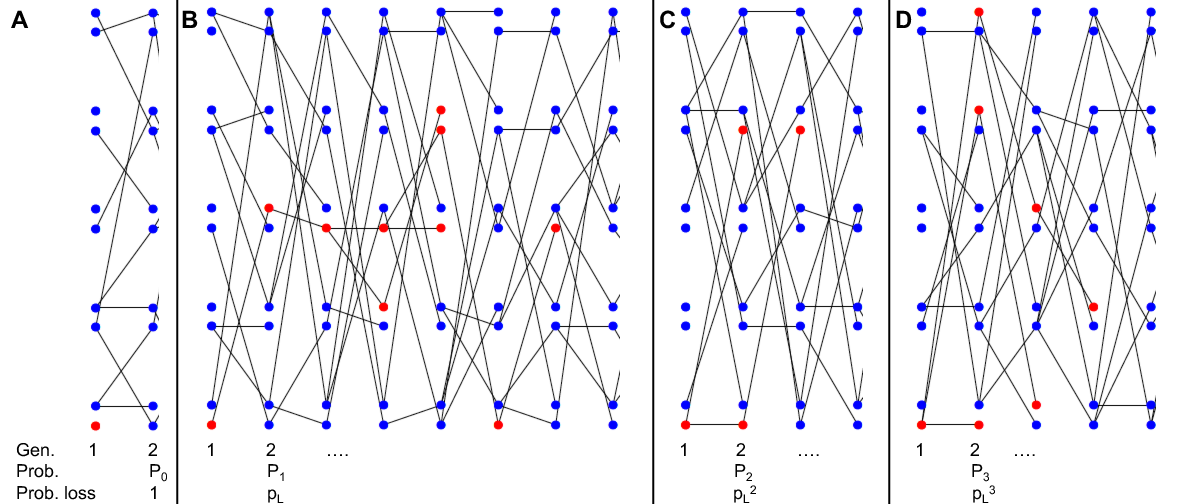
\includegraphics[width=\textwidth]{figures/Proof_of_pL_2s.png}
\end{center}
\caption{} \label{fig:Proof_of_pL_2s}
\end{figure}

%%consider reparameterizing 1+(1-hs)s
We can also adapt this result to a diploid setting.
Assuming that heterozygotes for the $1$ allele have $1+(1-h)s$ children, the
probability of allele $1$ is not lost, starting from a single copy in
the population, is
\begin{equation}
p_F = 2 (1-h)s \label{eqn:diploid_escape}
\end{equation}
for $h>0$. Note this is a slightly different parameterization from
our diploid model above.\\


\begin{tcolorbox} 
\begin{question}
Melanic squirrels suffer a higher rate of predation (due to hawks) than normally pigmented squirrels. Melanism is due to a dominant, autosomal mutation. The frequency of melanic squirrels at birth is $4 \times 10^{-5}$.\\

{\bf A)} If the mutation rate to new melanic alleles is $10^{-6}$,
assuming the melanic allele is at mutation-selection equilibrium, what
is the reduction in fitness of the heterozygote? \\ 
Suddenly levels of pollution increase dramatically in our population,
and predation by hawks now offers an equal (and opposite) advantage to
the dark individuals as it once offered to the normally pigmented
individuals. \\
{\bf B)} What is the probability that a single copy of this allele
(present just once in the population) is lost?\\ 
{\bf C)}  If the population size of our squirrels is a million
individuals, and is at mutation selection-balance, what is the probability that the population adapts from
anyone of these standing pool of melanic alleles?  
\end{question}
\end{tcolorbox}

\subsection{The interaction between genetic drift and weak selection.}
For strongly selected alleles, once the allele has escaped initial
loss at low frequencies, their path will be determined deterministically by their
selection coefficients. However, if selection is weak the
stochasticity of reproduction can play a role in the trajectory an
allele takes even when it is common in the population.\\

To see this lets think of our simple Wright-Fisher model (see R
exercise). Each generation we allow a deterministic change in our
allele frequency, and then binomially sample two alleles for each of
our offspring to construct our next generation.\\


%%%%%Include this discussion of sampling back in our HWE section??
%%%%%Next time

So the expected change in our allele frequency within a generation is given just by our
deterministic formula. To make things easy on our self lets assume an
additive model, i.e. $h=1/2$, and that $s \ll 1$ so that $\wbar
\approx 1$. This gives us
\begin{equation}
\E(\Delta p ) = \frac{s}{2} p(1-p) \label{eqn:WF_mean}
\end{equation}
our variance in our allele frequency change is given by
\begin{equation}
Var(p^{\prime} - p) = Var(p^{\prime}) = \frac{p^{\prime}(1-p^{\prime})}{2N}
\end{equation}
this variance in our allele frequency follows from the fact that we
are binomially sampling $2N$ new alleles in the next
generation from a frequency $p^{\prime}$. Denoting our count of allele $1$ by $i$ our
\begin{equation}
Var(p^{\prime} - p) = Var(\frac{i}{2N} - p) =  Var(\frac{i}{2N} ) =\frac{Var(i)}{(2N)^2}
\end{equation}
and from binomial sampling $Var(i) = 2N p^{\prime}(1-p^{\prime})$ and
so we arrive at our answer. Assuming that $s \ll 1$, $p^{\prime}
\approx p$, then in practice we can use
\begin{equation}
Var(\Delta p)  =Var(p^{\prime} - p) \approx \frac{p(1-p)}{2N}. \label{eqn:WF_var}
\end{equation}
To get our first look at the relative effects of selection vs drift we
can simply look at when our change in allele frequency caused
selection within a generate is reasonably faithfully passed across
the generations. In particular if our expected change in frequency is much
great than the variance around this change, genetic drift will play
little role in the fate of our selected allele (once the allele is not
too rare within the population). When does selected
dominant genetic drift? This will happen if $\E(\Delta p) \gg Var(\Delta p)$ when $Ns \gg 1$. Conversely any
hope of our selected allele following its deterministic path will be quickly undone if our change in allele frequencies due to selection is
much less than the variance induced by drift. So if $Ns \ll 1$ then
drift will dominate the fate of our allele. \\
\begin{figure}
\begin{center}
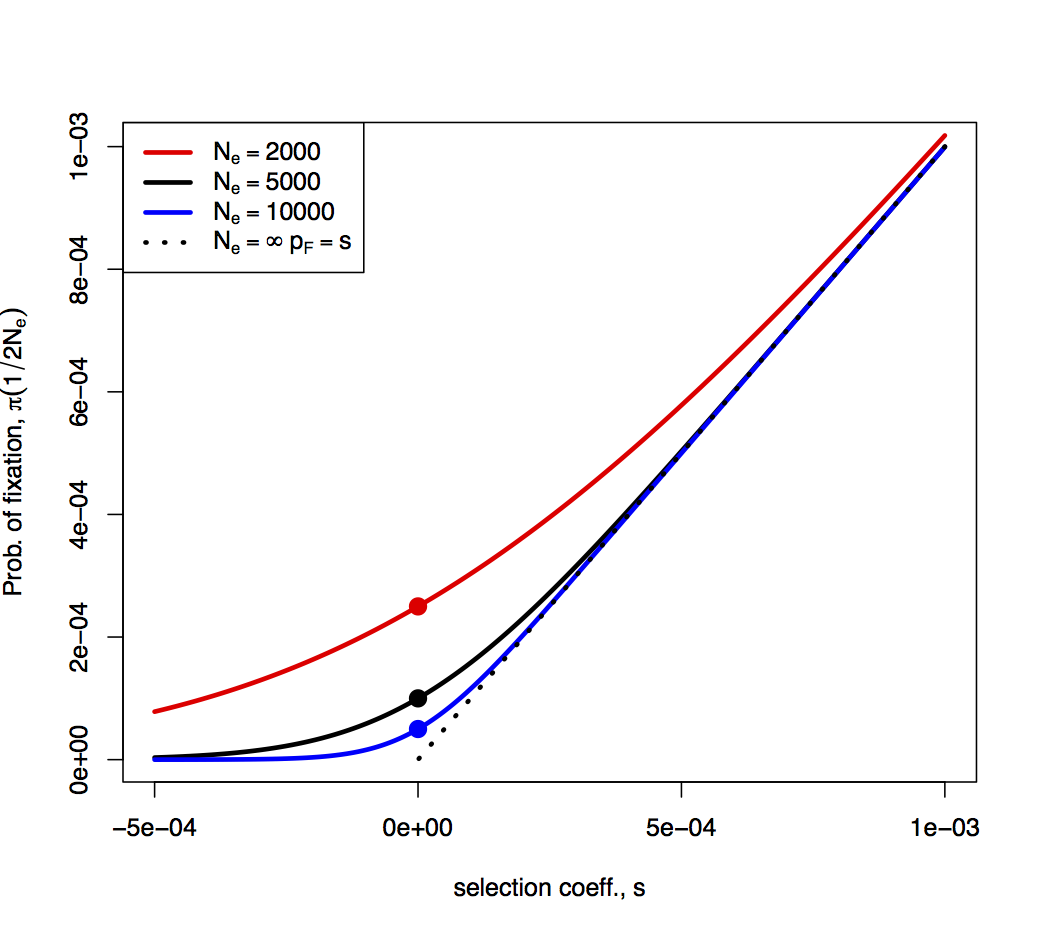
\includegraphics[width=0.6\textwidth]{figures/prob_fix_diffusion.png}
\end{center}
\caption{The probability of the fixation of a new mutation with
  selection coefficient $s$ ($h=1/2$) in a diploid population of effective
  size $N_e$. The dashed line gives the infinite population
  solution. The dots give the solution for $s \rightarrow 0$, i.e. $1/(2N_e)$} \label{fig:prob_fix_diffusion}
\end{figure}

To make further progress on understanding the fate of alleles with
selection coefficients of the order $1/N$ requires more careful
modeling. However, we can obtain the probability that under our diploid model, with an additive selection coefficient $s$, the
probability of allele $1$ fixing within the population starting
from a frequency $p$ is given by
\begin{equation}
\pi(p) = \frac{1-e^{-2Ns p }}{1-e^{-2Ns}} \label{eqn:prob_fixed}
\end{equation}
the proof of this is sketched out below (see Section \ref{Section:fixation_weakly_sel}). A new allele will arrive in the population at frequency $p=1/(2N)$,
then its probability of reaching fixation is
\begin{equation}
\pi \left(\frac{1}{2N} \right) = \frac{1-e^{-s }}{1-e^{-2Ns}} \label{eqn:new_mut_prob_fixed}
\end{equation}
if $s \ll1$ but $Ns \gg 1$ then $\pi(\frac{1}{2N}) \approx s$, which
nicely gives
us back our result that we obtained above
(eqn. \eqref{eqn:diploid_escape}). Our probability of fixation
(eqn. \eqref{eqn:new_mut_prob_fixed}) is plotted as a function of $s$
and $N$ in Figure \ref{fig:prob_fix_diffusion}. To recover our neutral
result we can take the
limit $s \rightarrow 0$ to obtain our neutral fixation
probability $1/(2N)$. \\

In the case where $Ns$ close to $1$ then
\begin{equation}
\pi \left( \frac{1}{2N} \right) \approx \frac{s}{1-e^{-2Ns}} \label{eqn:escape_from_intro}
\end{equation}
this is greater than our result $p_F=s$ from the branching process
argument (using our additive model of $h=1/2$), increasingly so for smaller $N$. 
Why is this?  The reason why is that $p_F$ is really the probability
of “never being lost” in an infinitely large population. So to persist
indefinitely the allele has to escape loss permanently, by never being
absorbed by the zero state. When the population size is finite, to fix
we only need to reach a size 2N individuals. Weakly beneficial
mutations (Ns~1) are slightly more likely to fix than the s
probability, as they only have to reach 2N to never be lost.


%Well in small populations selected alleles spend a
%somewhat shorter time segregating (especially at low frequencies), and so are
%slightly less susceptible to genetic drift. \\

\subsubsection{The fixation of slightly deleterious alleles.}
From Figure \ref{fig:prob_fix_diffusion} we can see that weakly
deleterious alleles can fix, especially in small populations.  To understand how
likely it is that deleterious alleles accidently reach fixation by
genetic drift, lets assume a diploid model with additive selection (with
a selection coefficient of $-s$ against our allele $2$).  
If $N s \gg 1$ then our deleterious allele (allele $2$) can not possibly reach
fixation. However, if $Ns$ is not large then
\begin{equation}
\pi \left( \frac{1}{2N} \right) \approx \frac{s}{e^{2Ns}-1} \label{eqn:fix_deleterious}
\end{equation}
for our deleterious allele. So deleterious alleles can fix within
populations (albeit at a low rate) if $Ns$ is not too large. As above
this is because while deleterious mutations will never escape loss in
infinite population, but they can become fixed in finite population by
reach 2N copies. This is captured by the denominator of the fixation
probability under the diffusion model, which that this increases the
fixation prob. of alleles with |Ns|~1. The absorption of alleles at 2N
copies can also be modeled in finite individual models (i.e. not the
diffusion limit), but we will not go into that here. 


\begin{tcolorbox} 
\begin{question}
`Haldane's sieve’ is the name for the idea that the mutations that contribute to adaptation are likely to be dominant or at least co-dominant. \\
{\bf A)} Briefly explain this argument with a verbal model relating to the
results we’ve developed in the last two chapters. \\
{\bf B)} Haldane’s sieve is thought to be less important for adaptation from previously deleterious standing variation, than adaptation from new mutation. Can you explain the intuition behind of this idea?\\
{\bf C)} Haldane’s sieve is likely to be less important in inbred,
e.g. selfing, populations. Why is this? \\
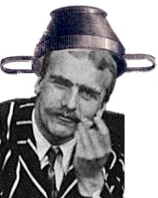
\includegraphics[width=0.1\textwidth]{figures/haldanes_sieve.png}

\end{question}
\end{tcolorbox}



\subsubsection{A Sketch Proof of the probability of fixation of
weakly selected alleles} \label{Section:fixation_weakly_sel}
%Kolmogorov backward eqn. 1931
%Kimura, M. 1962 On the Probability of Fixation of Mutant Genes in a
%Population. for abitrary dominance in diffusion.

We'll let $P(\Delta p)$ be the probability that our allele frequency
shifts by $\Delta p$ in the next generation. Using this we can write our probability $\pi(p)$ in terms of the probability of
achieving fixation averaged over the frequency in the next generation
\begin{equation}
\pi(p)  = \int \pi(p+\Delta p) P(\Delta p) d(\Delta p) \label{eqn:prob_fix_diff_step1}
\end{equation}
This is very similar to the technique that we used deriving our
probability of escaping loss in a very large population above. \\

So we need an expression for $\pi(p+\Delta p)$. To obtain this we'll
do a Taylor series expansion of $\pi(p)$ assuming that $\Delta p $ is small
\begin{equation}
\pi(p+\Delta p) \approx \pi(p) + \Delta p \frac{d\pi(p)}{dp} + (\Delta p)^2
\frac{d^2\pi(p)}{dp^2} (p)
\end{equation}
ignoring higher order terms.\\

Taking the expectation over $\Delta p $ on both sides, as in
eqn. \ref{eqn:prob_fix_diff_step1}, we obtain
\begin{equation}
\pi(p) = \pi(p) + \E(\Delta p) \frac{d\pi (p)}{dp} + \E((\Delta p)^2)
\frac{d^2\pi(p)}{dp^2}
\end{equation}

Well $\E(\Delta p) = \frac{s}{2}p(1-p)$ and $Var(\Delta p)= \E((\Delta
p)^2)-\E^2(\Delta p)$, so if $s \ll 1$ then $\E^2(\Delta p) \approx
0$, and $\E(\Delta p)^2 = \frac{p(1-p)}{2N}$. This leaves us with
\begin{equation}
0= \frac{s}{2}p(1-p)\frac{d\pi (p) }{dp} + \frac{p(1-p)}{2N}
\frac{d^2\pi (p) }{dp^2}
\end{equation}
and we can specify the boundary conditions to be $\pi(1)=1$ and $\pi(0)=0$. 
Solving this differential equation is somewhat involved process but in
doing so we find that
\begin{equation}
\pi(p) = \frac{1-e^{-2Ns p }}{1-e^{-2Ns}}
\end{equation}
This proof can be extended
to alleles with arbitrary dominance, however, this does not lead to a
analytically tractable expression so we do not pursue this here. 


%\section{Genetic drift and Neutral alleles}



\subsection{The fixation of neutral alleles}
It is very unlikely that a rare neutral allele accidentally drifts up
to fixation, it is much more likely that such an allele is eventually
lost from the population. However, there is a large and constant influx of
rare alleles into the population due to mutation, so even if it is very
unlikely that an individual allele fixes within the population, some
neutral alleles will fix.  \\

%We'll first consider the probability that a neutral allele fixes
%within the population, starting from it just enters a diploid
%population as a newly mutated allele at frequency $1/(2N)$.

%so for an allele to be fixed in the population it
%must have been that allele


\paragraph{Probability of the eventual fixation of a neutral allele.} An allele which reaches fixation within a population, is an ancestor to
the entire population. In a particular generation there can be only single
allele that all other alleles at the locus in  later generation can claim as an
ancestor. As at a neutral locus all of our alleles are exchangeable, as
they have no effect on the number of descendents an individual
leaves, so any allele is equally likely to be the ancestor of the
entire population.  In a diploid population size of size $N$, there are $2N$
alleles all of which are equally likely to be the ancestor of the
entire population at some later time point. So if our allele is present in a single copy, the chance that
is the ancestor to the entire population in some future generation is
$1/(2N)$, i.e. the chance our neutral allele is eventually fixed is
$1/(2N)$.\\

More generally if our neutral allele is present in $i$ copies in the
population, of $2N$ alleles, the probability that this allele is fixed
is $i/(2N)$. I.e. the probability that a neutral allele is eventually
fixed is simply given by its frequency ($p$) in the population.
We can also derive this result by letting $Ns \rightarrow
0$ in eqn. \eqref{eqn:prob_fixed}.

\paragraph{Rate of substitution of neutral alleles.}

A substitution between populations that do not exchange gene flow is
simply a fixation event within one population. The rate of
substitution is therefore the rate at which new alleles fix in the
population, so that the long-term substitution rate is the rate at
which mutations arise that will eventually become fixed within our population.\\

Assume that there are two classes of mutational changes that can occur with a
region, highly deleterious mutations and neutral mutations. A fraction
$C$ of all mutational changes are highly deleterious, and can not
possibly contribute to substitution nor polymorphism (i.e. $Ns \gg 1$).
While a fraction $1-C$ are neutral. If our mutation rate is $\mu$ per
transmitted allele per generation, then a total of $2N \mu (1-C)$
neutral mutations enter our population each generation.\\

Each of these neutral mutations has a $1/(2N)$ probability chance of
eventually becoming fixed in the population. Therefore, the rate at
which neutral mutations arise that eventually become fixed within our
population is  
\begin{equation}
2N\mu(1-C)\frac{1}{2N} = \mu(1-C)
\end{equation}
thus the rate of substitution under a model where newly arising alleles are either
highly deleterious or neutral, is simply given by the mutation rate
towards neutral alleles, i.e. $\mu(1-C)$.\\

Consider a pair of species have diverged for $T$ generations, i.e. orthologous sequences shared between the species last shared a common ancestor $T$ generations ago. If they have maintained a constant $\mu$ over that time, will have accumulated an average of
\begin{equation}
2\mu(1-C)T
\end{equation}
neutral substitutions. This assumes that $T$ is a lot longer than the time it
takes to fix a neutral allele, such that the total number of 
alleles introduced into the population that will eventually fix is the
total number of substitutions. We'll see below that a neutral allele
takes on average $4N$ generations to fix from its introduction into
the population.\\

This is a really pretty result as the population size has completely
canceled out of the neutral substitution rate. However, there is
another way to see this in a more straightward way. If I look at a
sequence in me compared to say a particular chimp, I'm looking at the mutations
that have occurred in both of our germlines since they parted ways $T$
generations ago. Since neutral alleles do not alter the probability
of their transmission to the next generation, we are simply looking at
the mutations that have occurred in $2T$ generations worth of
transmissions. Thus the average number of neutral mutational
differences separating our pair of species is simply $2\mu (1-C) T$.\\




\subsection{Comparing polymorphism and divergence}


\subsection{Deviations from the constant population model.}
We've seen previously that changes in our population size can be
captured by an effective population size. However, this will only be a
useful measure if population sizes vary rapidly enough, that the
harmonic mean effective population size over short time periods ($\ll
N_e$ generations) is representative of the effective population size averaged over
longer time periods. If this is not the case there is no one effective
population size, as we can not approximate our rate of drift by a
single constant population. Furthermore, we've ignored the effect of
population structure and selection which will violate our modeling
assumptions. \\

We can hope to detect violations from our constant population size
neutral model, by comparing aspects of our dataset to their expectations
and distributions under our neutral model. \\

For example we have devised two estimates of $\theta$,
$\widehat{\theta_{\pi}}$ and $\widehat{\theta_{W}}$, using
expectations of different aspects of our data (pairwise diversity and
number of segregating sites respectively). Under our constant neutral
model if we have sufficient data those two estimates should be
equal to each other on average. But if there's some violation of our model they might not
be. So one test statistic might be to take
\begin{equation}
D = \widehat{\theta_{\pi}} - \widehat{\theta_{W}}
\end{equation}
which will be zero in expectation if our data was generated by a
neutral constant population model.




\newpage

\chapter{The effect of linked selection on patterns of neutral diversity}

A newly derived allele with an additive selection coefficient $s$ will
take a time $\tau \approx 4\log(2N)/s$ generations to reach to fixation
within our population (see eqn. \eqref{eq:diploid_fix_time}). This short time window offers very little time
for recombination between the selected site and linked neutral
sites.  \\

First lets imagine examining variation at a locus fully linked
to our selected locus, just after our sweep reached fixation. A pair of neutral alleles sampled at this locus
must both trace their ancestral lineages back through to the neutral
allele on whose background the selected allele initially arose. As
that neutral allele, which existed $\tau$ generations ago is the
ancestor of the entire population at this locus. Our individuals who
carry the beneficial allele are, from the perspective of these two
alleles, exactly like a rapidly expanding population. Therefore, our
pair of neutral alleles sampled at our locus will be forced to
coalesce $\approx \tau$ generations ago. This is a very
short-time scale compared to the average neutral coalescent tie of
$2N$ generations of a pair of alleles.\\

If we now allow recombination into our model we can think about a pair
of alleles sampled at a neutral locus a recombination distance $r$
away from our selected site. Our pair of alleles will be forced to
coalesce $\approx \tau$ generations if neither of them reside on
haplotypes that the selected allele recombined onto during the
sweep. This is equivalent to saying that neither of our neutral
alleles recombine off of the beneficial allele's background moving
backward in time.\\

The probability that our lineage fail recombines off our beneficial
allele's background and onto the
ancestral background in the $j^{th}$ generation back is
\begin{equation}
r (1-X(j))
\end{equation}
so the probability ($p_{NR}$) that our lineage fails to recombine off in the
$\tau$ generations it takes our selected allele to move through the
population is
\begin{equation}
p_{NR}=\prod_{j=1}^{\tau} \big(1- r(1-X(j))\big)
\end{equation}
assuming that $r$ is small then $ \left(1- r(1-X(j))\right) \approx
e^{-r(1-X(j))}$, such that
\begin{equation}
p_{NR}=\prod_{j=1}^{\tau} \left(1- r(1-X(j))\right) \approx \exp
\left( -r\sum_{j=1}^{\tau}
1- X(j) \right) =\exp
\left( -r \tau (1-\widehat{X}) \right)
\end{equation}
where
$\widehat{X}$ is the average frequency of the derived allele across the trajectory
$\widehat{X} = \frac{1}{\tau}  \sum_{j=1}^{\tau}
 X(j)$. As our allele is additive its trajectory for frequencies
 $<0.5$ is the mirror image of its trajectory for frequency $>0.5$, therefore it
average frequency $\widehat{X} =0.5$. So
\begin{equation}
p_{NR} = e^{-r \tau/2 }.
\end{equation}
The probability that both of our lineages fail to recombine off the
sweep and hence are forced to coalesce is $p_{NR}^2$, assuming that
they coalesce at a time close to $\tau$ so that they recombine
independently of each other for times $< \tau$.\\

If one or other of our lineages recombine off the sweep it will take them on average
$\approx 2N$ generations to find a common ancestor as we are back our
neutral coalescent. Thus the expected time
till our pair of lineages find a common ancestor is
\begin{equation}
\E(T_2)  = \tau \times p_{NR}^2 +(1-p_{NR}^2) (\tau +2N) \approx
\left(1-p_{NR}^2 \right) 2N
\end{equation}
where this last approximation assumes that $\tau \ll 2N$. So the
expected pairwise diversity for neutral alleles at a recombination
distance $r$ away from the selected sweep  ($\pi_r$) is
\begin{equation}
\E(\pi_r) = 2\mu \E(T_2)  \approx \theta \left(1-e^{-r\tau} \right) \label{eqn:pi_HH}
\end{equation}
so diversity increases as we move away from the selected site,
slowly exponentially plauteuing to its neutral expectation $\theta=4N\mu$.\\

To get a sense of the physical scale over which diversity is reduced
consider a region where recombination occurs at a rate $r_{BP}$ per
base pair per generation, and our locus is $ \ell $ base pairs away from the
selected site $r=r_{BP } \ell $ (where $r_{BP}  \ell  \ll 1$ so we don't need to
worry about more than one recombination event occurring per
generation). Typical
recombination rates are on the order of $r_{BP} = 10^{-8}$, in Figure
\ref{fig:hitchhiking_reduction} we show the reduction in diversity,
given by eqn. \eqref{eqn:pi_HH}, for two different selection coefficients.\\ 

For our expected diversity levels to recover to $50\%$ of
its neutral expectation $\E(\pi_r)/\theta=0.5$, requires a physical
distance $\ell^{*}$ such that $\log(0.5) = -r_{BP} \ell ^*\tau$ as using our
expression for $\tau$ then $ \ell^* = \frac{-\log(0.5)}{r_{BP} \tau }$. As
$\tau$ depends inversely on the selection $s$ (eqn. \eqref{eq:diploid_fix_time}), the width of our trough of reduced diversity depends on $s/r_{BP}$.
All else being equal we expect stronger sweeps or sweeps in regions of low
recombination to have a larger hitchhiking effect. So that a selection coefficient of $s=0.1\%$ would reduce
diversity over 10's of kb, while a sweep of $s=1\%$ would affect
$\sim$100kb.   \\


\begin{figure}
\begin{center}
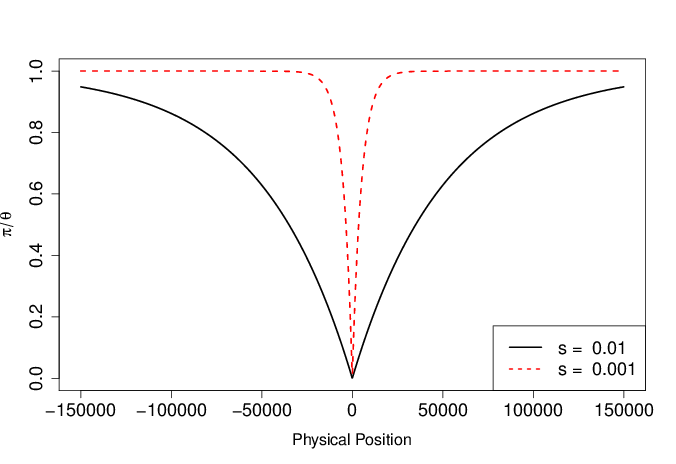
\includegraphics[width=0.5\textwidth]{figures/hitchhiking_reduction.png}
\end{center}
\caption{Reduction in diversity compared to its neutral expectation as
a function of the distance away from a site where a selected allele
has just gone to fixation. The recombination rate is $r_{BP}= 1\times
10^{-8}$.} \label{fig:hitchhiking_reduction}
\end{figure}

\begin{question}
A recently published study has identified the genetic basis of
melanism in the pepper moth. This allele swept to fixation in northern
parts of the UK; a classic case of adaptation to industrial pollution
(made famous by the work of Kettlewell). The genetic basis of melanism
is a transposable element (TE) inserted into a pigmentation gene. The
investigators found that diversity is suppressed in a broad region
around the TE. Specifically, on the background of the TE, it takes
roughly 200 kb in either direction for diversity levels to recover to
50\% of genome-wide levels. \\

Random facts: In all moths and butterflies only males recombine;
chromosomes are transmitted without recombination in female. The
recombination rate in males is 2.9 cM/Mb.  Peppered moths have an
effective population size of roughly a hundred thousand
individuals. Kettlewell used to eat moths when out collecting them in
the field (personal communication, Art. Shapiro). \\
{\bf A)} Briefly explain how this pattern offers further evidence that the melanic allele was favoured by selection.\\
{\bf B)} Using this information what is your estimate as to the age of the allele?\\
{\bf C)} What is your estimate of the selection coefficient favouring this melanic?
\end{question}


\subsection{A simple recurrent model of selective sweeps}
We sample a pair of neutral alleles at a locus a genetic distance $r$ away from a locus where
sweeps are initiated within the population at some very low rate $\nu$
per generation. The waiting time between sweeps
at our locus is exponential $\sim Exp(\nu)$. Each sweep rapidly transits through the population in $\tau$
generations, such that each sweep is finished long before the next
sweep ($\tau \ll 1/\nu$). \\

As before our chance that our neutral lineage fails to recombine
off the sweep is $p_{NR}$, such that the probability that
our pair of lineages are forced to coalesce by a sweep $e^{-r \tau}$. Our
lineages therefore have a very low probability
\begin{equation}
\nu e^{-r \tau}
\end{equation}
of being forced to coalesce by a sweep per generation. In addition of
lineages can coalesce at a neutral rate of $1/(2N)$. Thus the average
waiting time till a coalescent event between our neutral pair of
lineages due to either a sweep or a neutral coalescent event is
\begin{equation}
\E(T_2) = \frac{1}{\nu e^{-r \tau} + 1/(2N)}
\end{equation}

Now imagine that the sweeps don't occur at a fixed location with
respect to our locus of interest, but now occur uniformly at random
across our sequence. The sweeps are initiated at a very low rate of
$\nu_{BP}$ per basepair per generation. The rate of coalescent due to
sweeps at a locus $\ell$ basepairs away from our neutral loci is
$\nu_{BP} e^{-r_{BP} \ell \tau}$. If our neutral locus is in the
middle of a chromosome that stretches $L$ basepairs in either direction
the total rate of sweeps per generation that force our pair of lineages to coalesce is
\begin{equation}
2\int_0^{L} \nu_{BP} e^{-r_{BP} \ell \tau} d \ell =
\frac{2\nu_{BP}}{r_{BP} \tau} \left(1-e^{-r_{BP} \tau L} \right)
\end{equation}
so that if $L$ is very large ($r_{BP} \tau L \gg 1$) the rate of coalesce per
generation due to sweeps is $\frac{2\nu_{BP}}{r_{BP} \tau}$. The total rate
of coalescence for a pair of lineages per generation is then
\begin{equation}
\frac{2\nu_{BP}}{r_{BP} \tau}+\frac{1}{2N}
\end{equation}
So our average time till a pair of lineages coalesce is
\begin{equation}
\E(T_2) = \frac{1}{\frac{2\nu_{BP}}{r_{BP} \tau}+\frac{1}{2N}} = \frac{r_{BP}2N}{\frac{4N\nu_{BP}}{ \tau}+r_{BP}}
\end{equation}
such that our expected pairwise diversity ($\pi=2\mu\E(T_2)$) in a region of
recombination rate $r_{BP}$ that experiences sweeps at rate $\nu_{BP}$
is  
\begin{equation}
\E(\pi) = \theta \frac{r_{BP}}{\frac{4N\nu_{BP}}{ \tau}+r_{BP}} \label{eqn:pi_GW_HH}
\end{equation}


\begin{figure}
\begin{center}
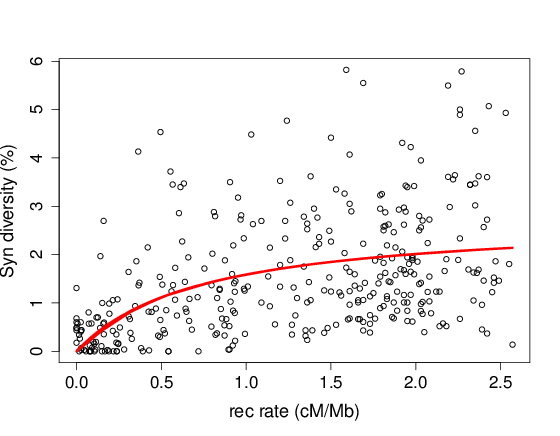
\includegraphics[width=0.5\textwidth]{figures/Genomewide_HH.png}
\end{center}
\caption{The relationship between (sex-averaged) recombination rate and synonymous
  site pairwise diversity ($\pi$) in {\it Drosophila melanogaster}
  using the data of Shapiro et al. 07 (kindly provided by Peter
  Andolfatto, see Sella et al. 09 for details). The curve is the
  predicted relationship between $\pi$ and recombination rate obtained
  by fitting equation \eqref{eqn:pi_GW_HH} to this data 
 using non-linear least squares via the {\tt nls()} function in {\tt R}.} \label{fig:GW_hitchhiking_reduction}
\end{figure}




\chapter{Interaction of Multiple Selected Loci}

Selection doesn't act on loci in isolation, and the fates of selected alleles in the genome are correlated. In the prior chapter we looked into how selected loci affected neutral loci. Here we'll explore the interaction of multiple selected loci. Throughout this chapter we'll see how multi-locus dynamics are key to understanding hypotheses about the evolutionary significance of sexual reproduction, after all the primary evolutionary costs and benefits of sex arise the independent assortment of chromosomes and recombination. Multi-locus dynamics are also often key to understanding how new species arise and are maintained. From a population-genetic perspective, species are sets of traits and alleles held together by assortative mating and selection.

\section{Why sex?}
The vast majority of eukaryotic organisms reproduce sexually. Sexual reproduction, the fusion of two cells to form a zygote  ({\it syngamy}) followed by meiosis, represents an ancient feature of eukaryotes. However, the ubiquity of sex is not just due to sex being a fixed ancestral state of eukaryotes. Many eukaryotic species are not obligately sexual and can reproduce clonally (i.e. asexually), e.g. vegetative growth in plants. However, they will reproduce clonally only for a a short wgile before having sex again. There are even asexual vertebrate lineages. For example, there are a number of obligately parthenogenic species of whiptail lizard ({\it Aspidoscelis}), where every individual in the species is female and reproduce clonally.  However, only a small fraction of  eukaryote species are obligate asexuals, and these species appear to be short-lived twigs on the eukaryotic tree of life. 

Sex reproduction is confined to eukaryotes but most non-eukaryotic species have some form of genetic exchange where genetic material is acquired and incorporation into their genomes via a range of mechanisms. These non-eukaryotic mechanisms often seem to have evolved in part because they facilitate genetic exchange 

Thus, sex and genetic exchange are incredibly widespread. Yet sex has substantial short-term costs. 

\paragraph{The costs of sex.}
Three broad costs of sex have often been hypothesized:
\begin{enumerate}
\item  {\emph The cost of mating}. Finding and attracting a mate are costly and may be impossible, and mating can be dangerous.
\item  {\emph The cost of recombination.} Why risk breaking it up a winning genotype? If you've managed to survive to reproduce you're genotype likely can't be a terrible fit to the environment. But if you engage in sexual reproduction, i.e. meiosis, you're shuffling up your genome with that of your partner. There's no guarantee that this new genotype will work well in the current environment. 
\item The  {\emph two-fold cost of sex} \citep{smith1971origin}. The offspring of sexual organisms have two parents. Therefore, sexual parents only contribute half of their genome to their offspring. While asexual organisms contribute their entire genome to the next generation. Thus a sexual organism has to have twice as many children to leave the same number of copies of their genome to the next generation. That might be doable if both sexual parents were equally committed to contributing to those offspring. However, that is rarely the case. This cost is sometimes called the {\emph two-fold cost of males}, as males often provide little in terms of resources to their children. Thus any allele that makes its host asexual should initially spread all else being equal. 
\end{enumerate}
Yet sex and other forms of genetic exchange persist, despite these short-term advantages to asexual reproduction. Indeed asexual lineages often arise and spread within some sexual populations due to these advantages. 

\paragraph{The benefits of sex.}
Numerous benefits to sexual reproduction have been suggested. Throughout this chapter we'll encounter a range of models that touch on the advantages of sex. We'll see that selection allows beneficial alleles to shed their background of deleterious alleles as they sweep through the population. In the absence of sex and recombination, beneficial alleles can block each other's progression to fixation, so called `clonal interference'. Another major advantage of sex is that beneficial alleles can be brought together on the same genetic background via recombination, allowing faster rates of adaptation. 

\section{A two locus model of selection and recombination.}
Models involving many selected loci can be very challenging to analyze. Luckily for us many of the key insights of the interaction of selection and recombination can be understood in relatively intuitive terms, and demonstrated using two locus models. 

Consider two biallelic loci segregating for $A/a$ and $B/b$. There are four haplotypes, $AB$, $Ab$, $aB$, $ab$, which for simplicity we label 1-4. The frequency of our four haplotypes are $x_1$, $x_2$, $x_3$, and $x_4$. Each individual has a genotype consisting of two haplotypes; we label $w_{ij}$ the fitness of an individual with the genotype made up of haplotype $i$ and $j$ (we assume that $w_{ij}=w_{ji}$, i.e. there are no parent of origin effects). Assuming that these fitnesses reflect differences due to viability selection, and that individuals mate at random, we can write the following table of our genotype proportions after selection:\\
\begin{center}
\begin{tabular}{c|cccc}
         & $AB$			& $Ab$				& $aB$				& $ab$\\
\hline
$AB$ & $w_{11} x_1^2$ 	& $w_{12} 2 x_1 x_2$  	& $w_{13} 2 x_1 x_3$ 	& $w_{14} 2 x_1 x_4$ \\
$Ab$ & $\bullet$ 	  	& $w_{22} x_2^2$ 	  	& $w_{23} 2 x_2 x_3$  	& $w_{24} 2 x_2 x_4$ \\  
$aB$ & $\bullet$ 		& $\bullet$ 			& $w_{33} x_3^2$ 	  	& $w_{34} 2 x_3 x_4$ \\  
$ab$ & $\bullet$ 		& $\bullet$			& $\bullet$ 			&  $w_{44} x_4^2$ \\
\end{tabular}
\end{center}
This follows from assuming that our haplotypes are brought together at random (HWE), then discounted by their fitnesses. Our mean fitness $\bar{w}$ is the sum of all the entries in the table, so dividing by $\bar{w}$ normalizes the complete table to sum to one. The frequency of the $AB$ haplotype ($1$) in the next generation of gametes is
\begin{equation}
x_1' = \frac{\big( w_{11} x_1^2 +	 \half w_{12} 2 x_1 x_2  + \half w_{13} 2x_1 x_3  +	 \half (1-r) w_{14} 2 x_1 x_4 + \half r w_{23} 2 x_2 x_3   \big)}{ \bar{w} } \label{eqn:hapfreq}
\end{equation}
This is a bit of a mouthful, but each of the terms is easy to understand. Each of the HWE genotype frequencies (e.g. $2x_1x_2$) is weighted by its fitness relative to the mean fitness ($w_{ij}/\bar{w}$), and by its probability of transmitting the AB haplotype to the next generation. For example, $AB/Ab$ individuals (1/2) transmit the $AB$ haplotype only half the time. The final two terms include the recombination fraction ($r$). The first term involving recombination refers to the $AB/ab$ genotype (1/4), who with probability $(1-r)/2$ transmits a non-recombinant $AB$ haplotype to the gamete. Similarly, the second term refers to the  $Ab/aB$ genotype; a proportion $r/2$ of its gametes carry the recombinant $AB$ haplotype. 

In the single locus case, we defined the marginal fitness of an allele. Here it will help us to define the marginal fitness of the $i^{th}$ haplotype:
\begin{equation}
\bar{w}_i = \sum_{j=1}^4 w_{ij} x_j
\end{equation}
This is the fitness of the $i^{th}$ haplotype averaged over all of the diploid genotypes it could occur in, weighted by their probability under random mating. Using this notation, and with some rearrangement of equation \eqref{eqn:hapfreq}, we obtain
\begin{equation}
x_1' = \frac{x_1\bar{w}_1 - w_{14} r D}{\bar{w}}
\end{equation}
Here we have assumed that $w_{23}=w_{14}$, i.e. that the fitness of $AB/ab$ individuals is the same as $Ab/aB$ individuals (i.e. that fitness depends only on the alleles carried by an individual, and not on which chromosome they are carried; this assumption is sometimes called no {\it cis}-epistasis). 

We can then write the change in the frequency of our $1$ haplotype as 
\begin{equation}
\Delta x_1= \frac{x_1(\bar{w}_1-\bar{w}) -r w_{14} D}{\bar{w}}
\end{equation}
Generalizing this result, we write the change in any haplotype i from our set of four haplotypes as
\begin{equation}
\Delta x_i= \frac{x_i(\bar{w}_i-\bar{w}) \pm r w_{14} D}{\bar{w}}  \label{eqn:two_loc_sel}
\end{equation}
where the coupling haplotypes 1 and 4 use $+D$ and repulsion haplotypes 2 and 3 use $-D$. \erin{I'm confused about the signs +/- here. For haplotype 1 above you used -rw14D but here you're saying it's +D. Also, why doesn't the sign of D itself take care of the +/- (I think this second part is just my own confusion, but the first part doesn't seem to match between the equation above and your text)} Note that the sum of these four $\Delta x_i$ is zero, as our haplotype frequencies sum to one.

So the change in the frequency of a haplotype (e.g. AB, haplotype 1) is determined by the interplay of two factors: First, the extent to which  the marginal fitness of our haplotype is higher (or lower) than the mean fitness of the population (the magnitude and sign of $(\bar{w}_1-\bar{w})/\bar{w}$). Second, whether there is a deficit or any excess of our haplotype compared to linkage equilibrium (the magnitude and sign of $D$), modified by the strength of recombination. This tension between selection promoting particular haplotypic combinations, and recombination breaking up overly common haplotypes is the key to a lot of interesting dynamics and evolutionary processes.

\section{Types of interaction between selection and recombination}
Throughout the rest of the chapter we'll discuss some general forms to the interactions between selected loci and how recombination plays into either facilitating or hindering selection. To illustrate these ideas we make use of Muller diagrams \citep{muller1932some}, where we visualize the allele dynamics in terms of a plot of the stack frequencies over time. All of our simulations use the same basic two locus dynamics given by eqn \eqref{eqn:two_loc_sel}. To keep things simpler we just discuss through the qualitative dynamics of these models, but many of these models have been investigated in much more depth.

\subsection{The hitchhiking of neutral alleles}
\begin{figure}
\begin{center}
  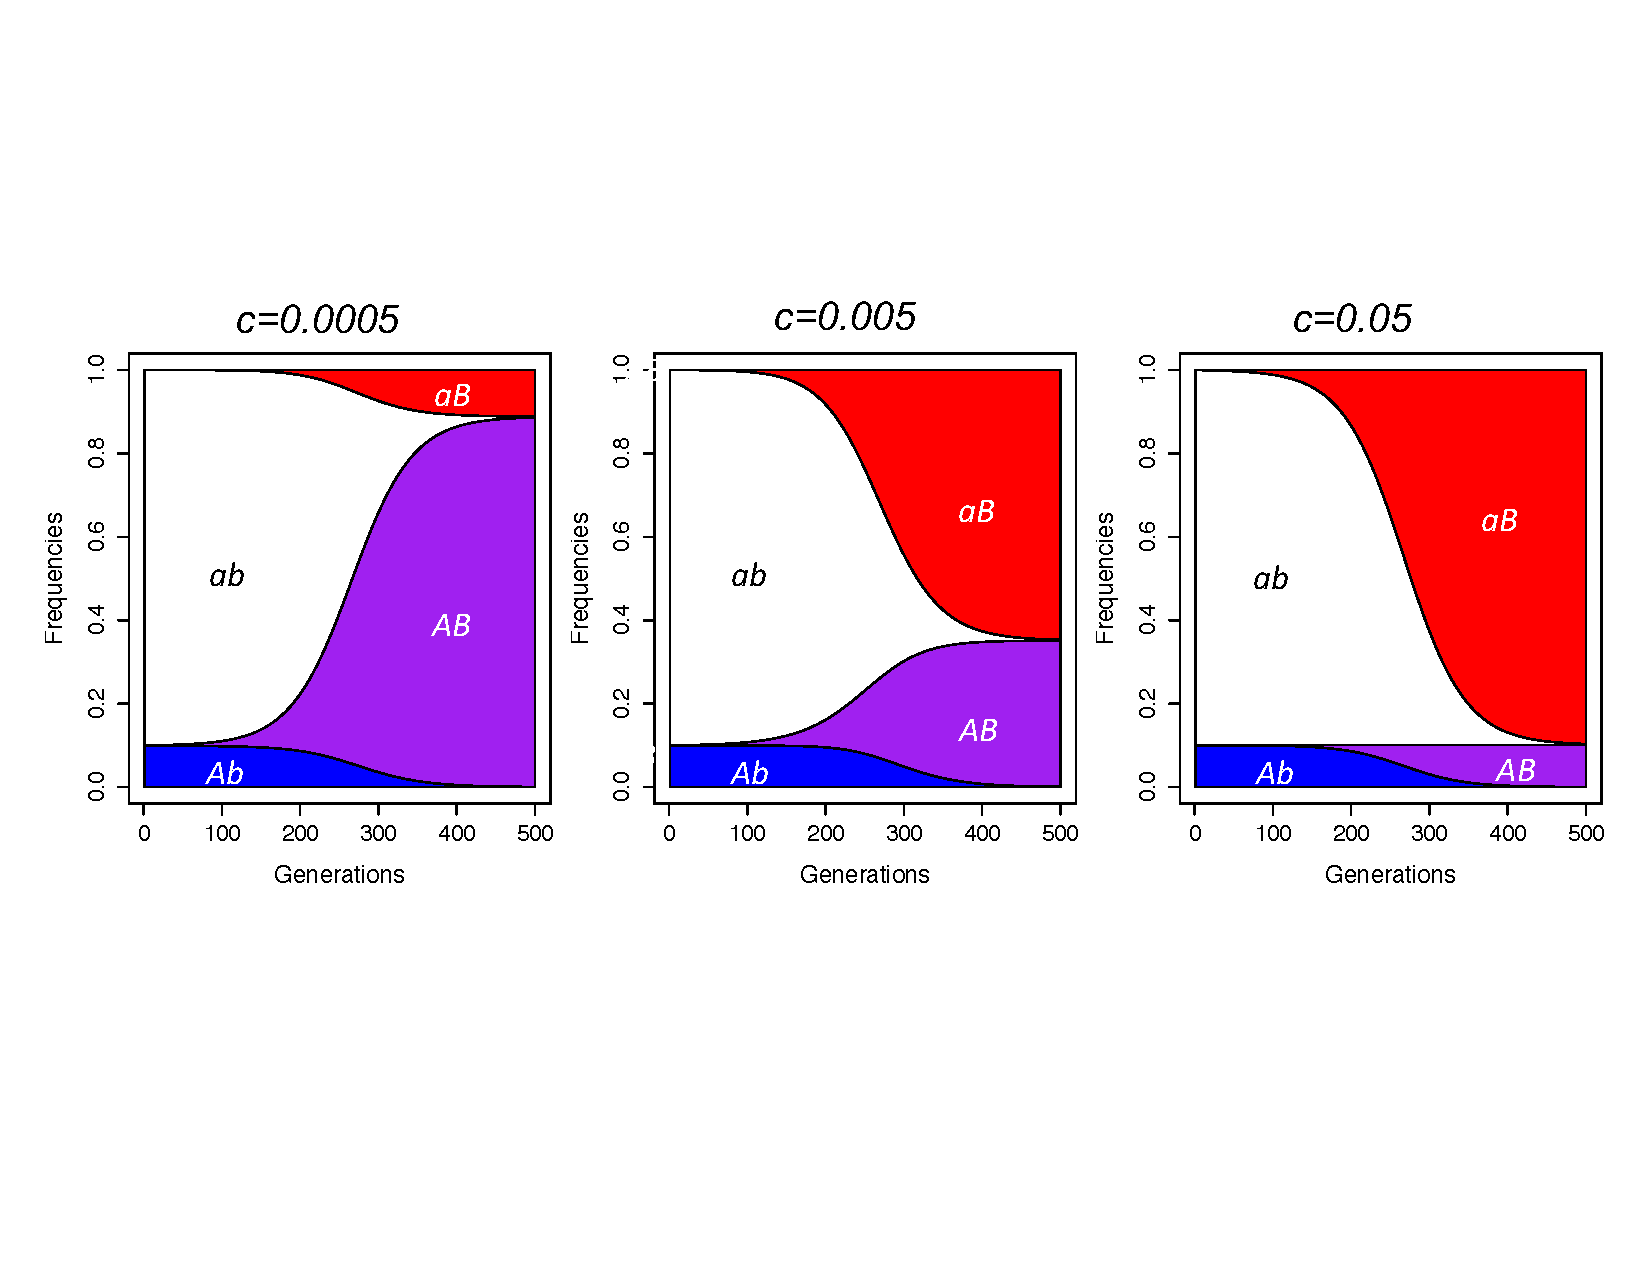
\includegraphics[width = 0.9 \textwidth]{figures/selection_recom_interaction/Neutral_Hitchhiking_labeled.pdf}
\end{center}
\caption{A beneficial mutation $B$ arises on the background of a neutral allele whose initial frequency is $p_A=10\%$. The beneficial allele has a strong, additive selection coefficient of $hs=0.05$.} \label{fig:Neutral_HH}  %é
\end{figure}
Let's start by revisiting our neutral hitchhiking in this two locus setting in the previous chapter we saw that neutral alleles can hitchhike along with our selected allele if they are tightly linked enough. Figure \ref{fig:Neutral_HH}  shows the frequency trajectories of the various haplotypes for neutral allele ($A$) that is present at $10\%$ frequency in the population when our beneficial allele ($B$) arises on its background. When the recombination rate ($r$) is low between the loci, $A$ gets to hitchhike to high frequency, but for higher recombination rates it only gets dragged to intermediate frequencies. For the highest recombination rate shown ($r \approx s$) the neutral allele's dynamics ($p_{Ab}+p_{AB}$) are barely changed at all, as it recombines on and off the sweeping allele frequently and so barely perceives the sweep. 

\subsection{The hitchhiking of deleterious alleles}
Deleterious alleles can also hitchhike along with beneficial mutations if they are not too deleterious compared to the benefits offered by the selected allele. Again our allele $A$ is at $10\%$ frequency in the population in Figure \ref{fig:deleterious_HH}, but this time it is deleterious and so initially decreasing in frequency across the generations when the beneficial mutation ($B$) arises on its background. If the loci are tightly linked, and A were too deleterious, B would never get to take off in the population.   However, if the benefits of B outweighs the cost of A, even in the case of no recombination between our loci, allele $A$ gets to hitchhike to fixation and merely slows down $B$'s rate of increase and their combined fitness is reduced. With moderate amounts of recombination between the loci, our deleterious starts to hitchhike but before it can get to fixation the beneficial allele manages to recombine off its background. This recombinant aB haplotype, which has higher fittest as it lacks the deleterious allele can now sweep through the population displacing the AB haplotype. For higher recombination events we have to wait less long for a recombination to breakup the hitchhiking deleterious allele, so the adaptive allele easily escapes its background.
For the purposes of illustration here we've used a relatively common deleterious allele, but in reality these alleles will likely be often be rare in the population and at mutation selection balance. If they are rare it is likely that a beneficial mutation arises on a specific deleterious allele's background, but as we have seen there are likely going to be many rare deleterious alleles in the population so it is likely that a beneficial mutations may often have to contend with deleterious hitchhikers. 
\begin{figure}
\begin{center}
  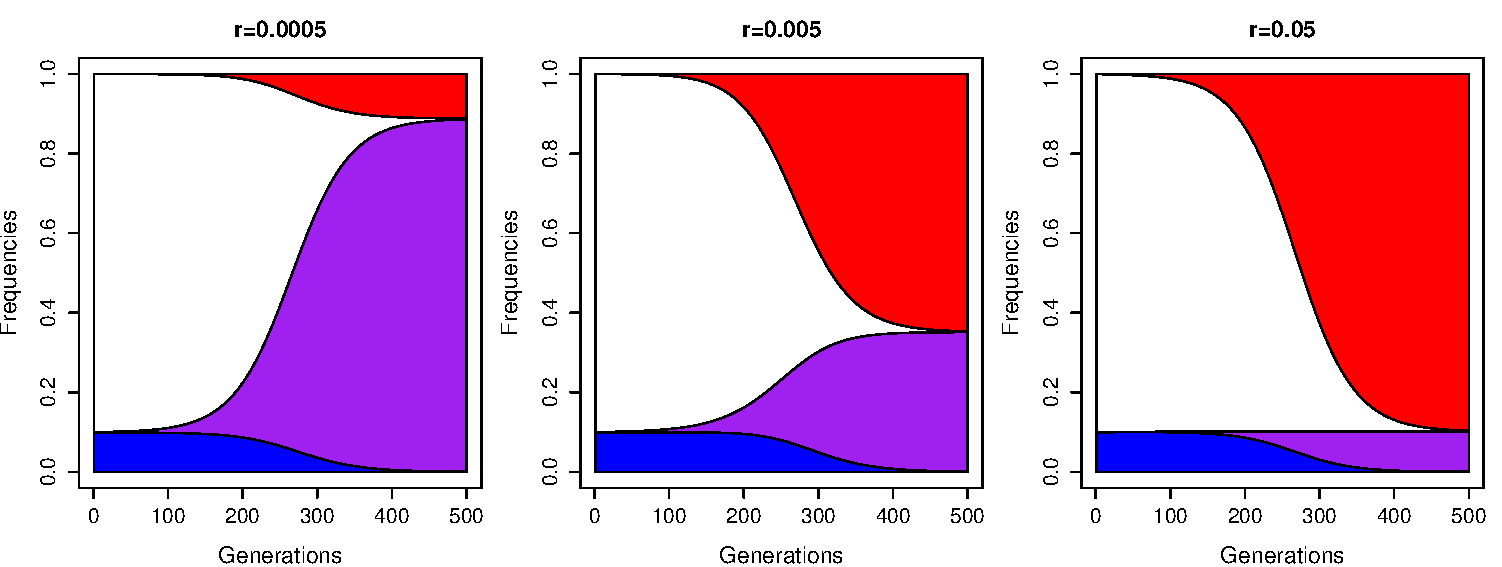
\includegraphics[width = 0.9 \textwidth]{figures/selection_recom_interaction/Deleterious_Hitchhiking.pdf}
  \caption{The hitchhiking of a deleterious allele. The beneficial allele B arises on the background of a deleterious allele A, and the extent to which the A allele gets to hitchhiking along depends on the recombination rate. \gitcode{https://github.com/cooplab/popgen-notes/blob/master/Rcode/two_locus_sel.R}} \label{fig:deleterious_HH}  %é
  \end{center}
\end{figure}


\begin{figure*}
\begin{center}
  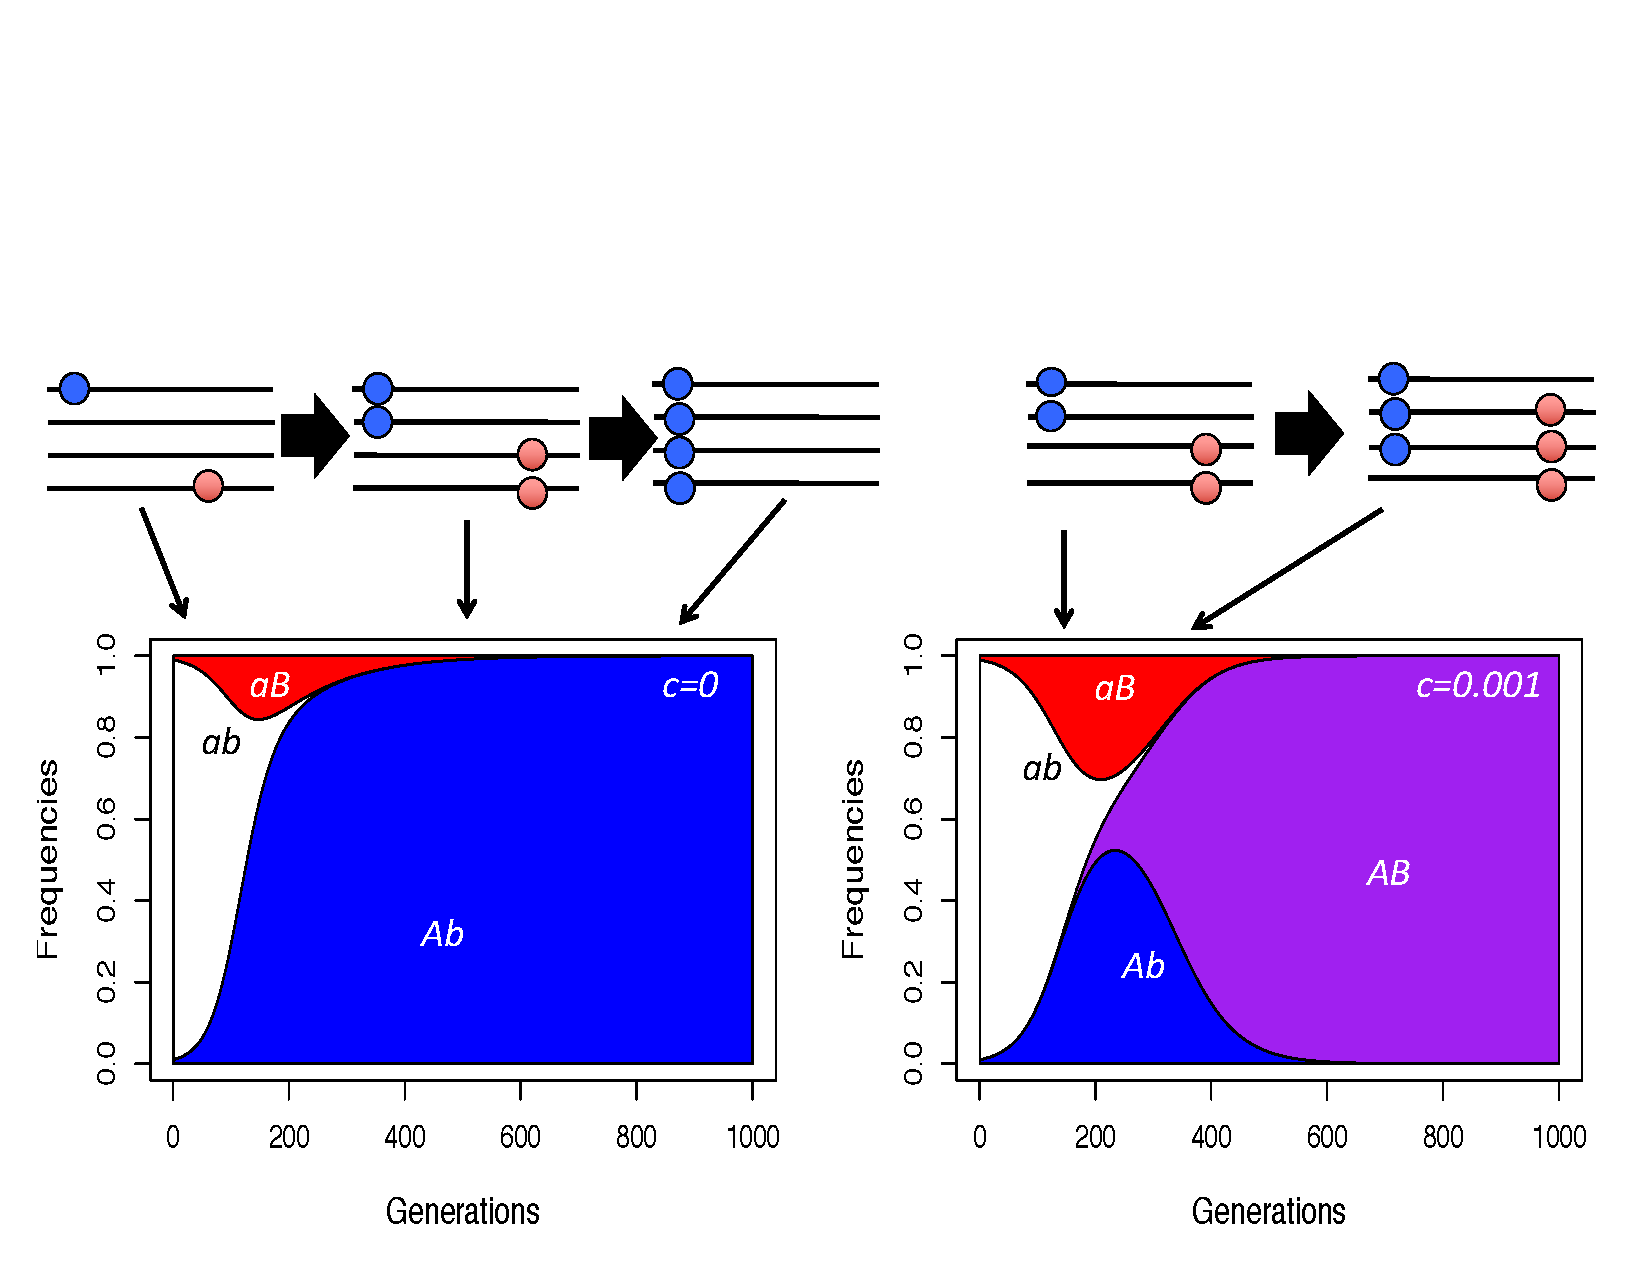
\includegraphics[width = 0.8 \textwidth]{figures/selection_recom_interaction/Interference_w_haps.pdf}
\end{center}
\caption{Interference between two positively selected alleles. {\bf Left)} the red and blue (A and B) beneficial alleles arise on different haplotypes. They rise in frequency, but in the absence of recombination only one can fix. This is shown in a Muller diagram, where $p_{AB}$ is initially set to zero. {\bf Right)} In the presence of recombination the population can generate the recombinant (AB) haplotype, which can subsequently fix. \gitcode{https://github.com/cooplab/popgen-notes/blob/master/Rcode/two_locus_sel.R}} \label{fig:Interference}  %é
\end{figure*}
\subsection{Clonal interference between favourable alleles.}
When rates of sex and recombination are zero, or very low, positively selected alleles can prevent each other reach fixation and so the rate of adaptation can be slowed.
In the absence of sex and recombination, when two positively selected alleles arise on different genetic backgrounds in the population they cannot both fix (left side of Figure \ref{fig:Interference}). They can initially increase in frequency, but necessarily compete with each other when they become common. This is called selective interference, or sometime clonal interference. If one of the alleles has a much larger selection coefficient it will fix, forcing the other allele from the population, but when they are relatively equally matched it may take some time for this situation to resolve itself resulting in a traffic jam in the population. Thus in an asexual adaptive alleles necessarily have to fix sequentially. However, with even a small amount of recombination beneficial alleles can recombine on to each others background, allowing them to fix in parallel (right side of  Figure \ref{fig:Interference}).   

\begin{marginfigure}
\begin{center}
  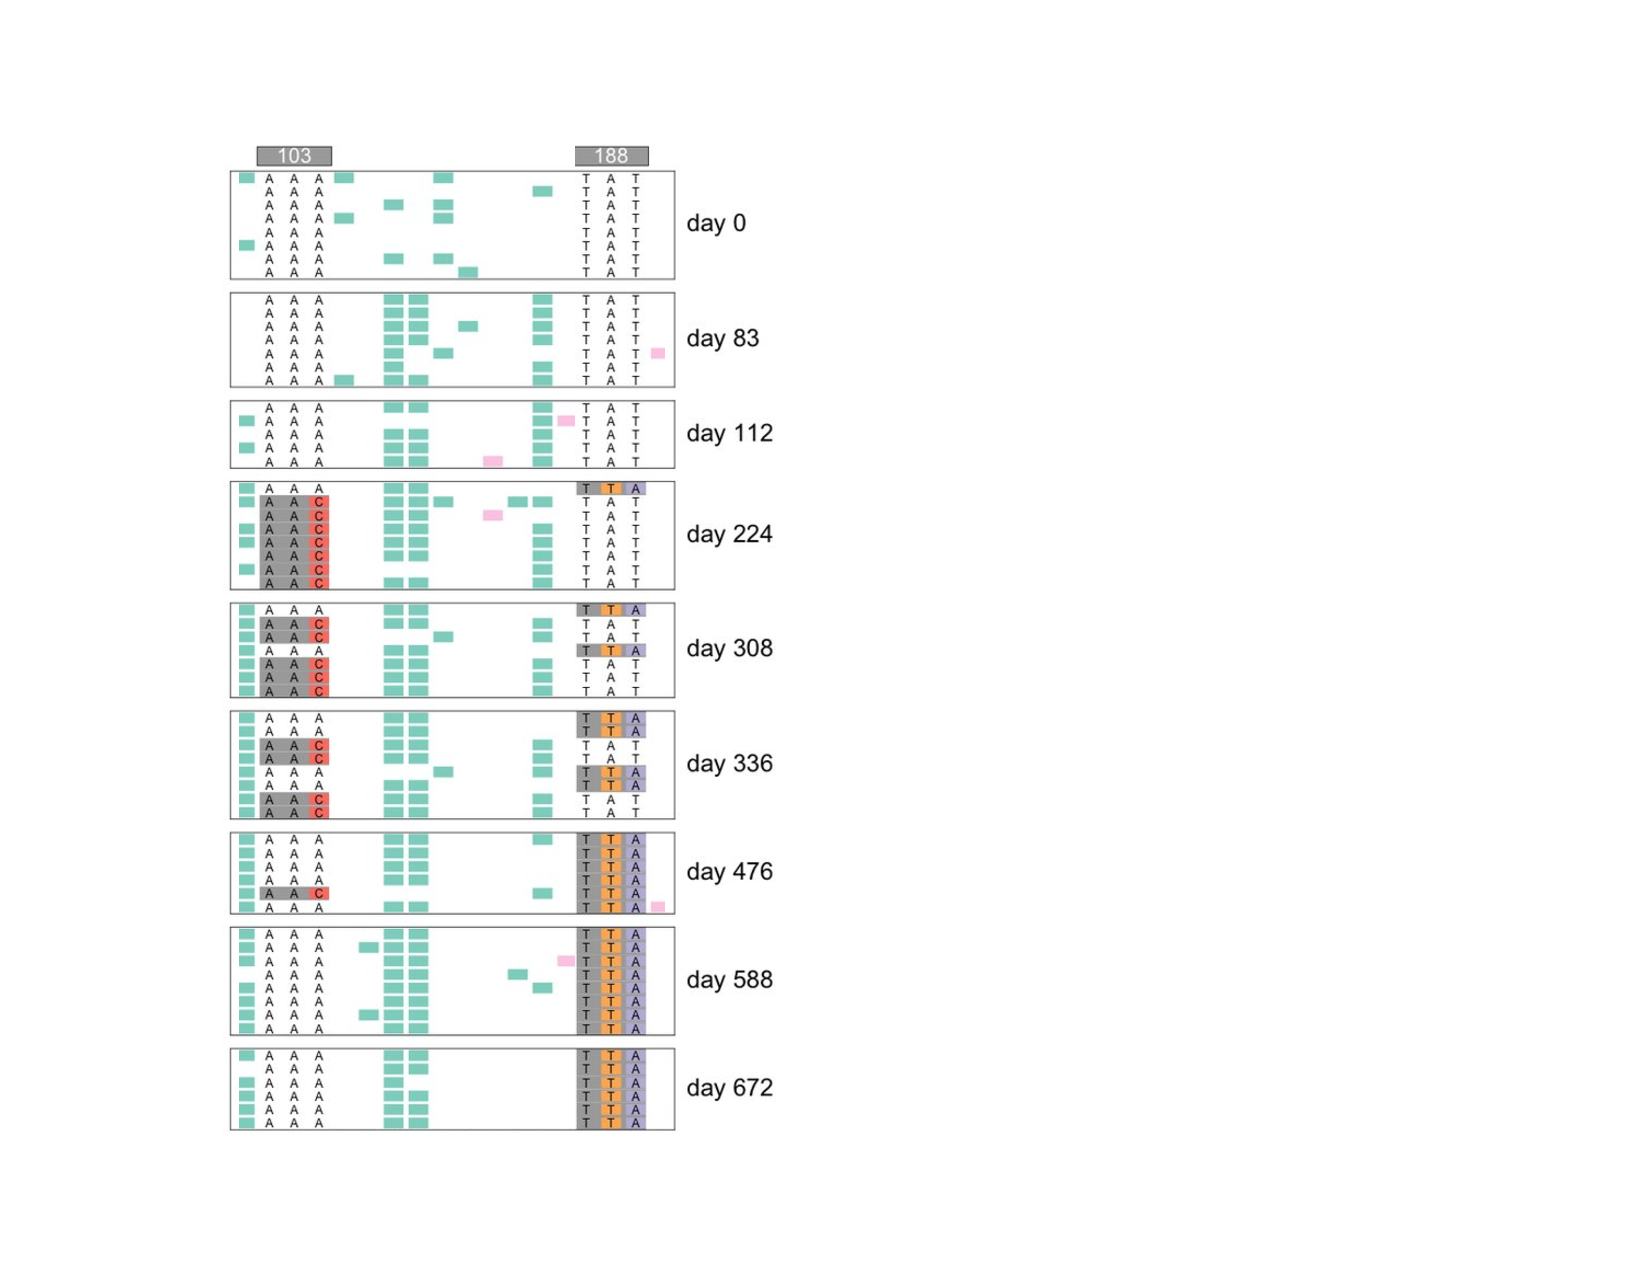
\includegraphics[width =  \textwidth]{Journal_figs/recom_selection/Pleuni_HIV_interference/Trimmed_HIV_interference}  %DdwdkVeVMAA7t-V.jpg}
\end{center}
\caption{HIV sequences from a patient over the course of drug treatment in the retrotransposase coding region. Figure cropped from \citet{Williams548198}, \PLOSccBY.} \label{fig:HIV_interference}  %é
\end{marginfigure}
Given the rapid evolution of HIV we can see interference taking place over very short time periods indeed. HIV uses its reverse transcriptase (RT) gene to write itself from an RNA virus into its host's DNA, allowing HIV to hijack the hosts regulatory machinery, a critical part of its life cycle. One of the early HIV drugs was Efavirenz, which inhibits HIV's RT protein. Sadly, mutations are common in the RT HIV gene, and these mutations, in the presence of the drug, confer a profound fitness advantage, allowing them to spread through the HIV population in patients undergoing anti-HIV treatment. In Figure \ref{fig:HIV_interference} we see that by day 224 after the start of drug treatment two different drug-resistance amino-acid changes beginning to spread within a patient (also shown as a Muller diagram in Figure \ref{fig:HIV_interference_M}). Because these alleles occur on different genetic backgrounds, with little chance for genetic exchange between them, they interfere in each other progress as they compete to fix within the population. Eventually the amino acid change at site 188 wins out. 

\begin{figure}
\begin{center}
  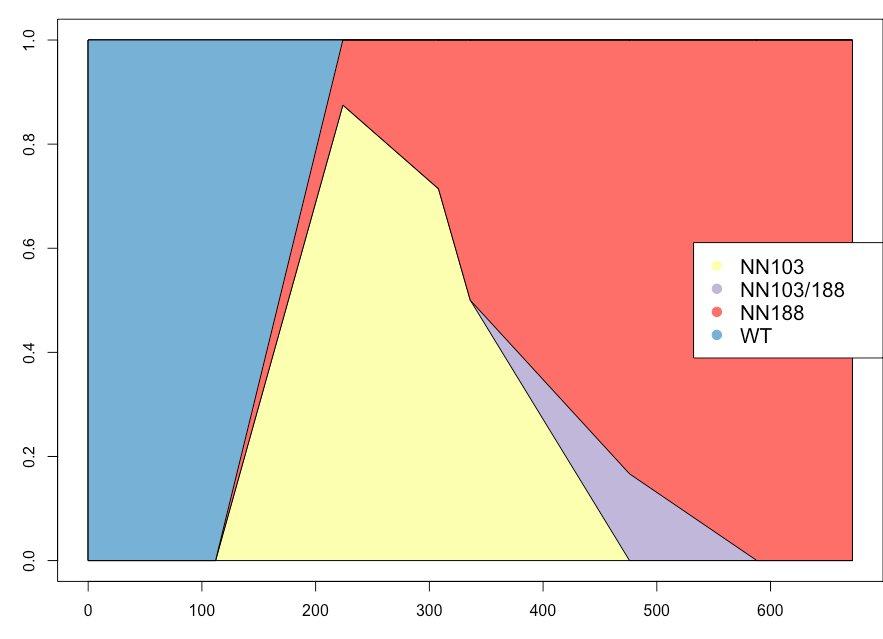
\includegraphics[width = \textwidth]{Journal_figs/recom_selection/Pleuni_HIV_interference/DdweQyxU0AA7mXe.jpg}
\end{center}
\caption[][3cm]{Muller plot of the drug resistance interference dynamics from Figure \ref{fig:HIV_interference}. Figure from \citet{Williams548198}, \PLOSccBY.} \label{fig:HIV_interference_M}  
\end{figure}

\subsection{Epistatic combinations of alleles and the cost of recombination.}
\marginnote{
  \begin{quote}
``Love, love will tear us apart again'' --Joy Division.
\end{quote}
}
Recombination comes at a cost. While recombination can bring beneficial combinations of alleles together, it will also tear them apart. To see this imagine a pair of alleles A and B at two loci that work very well together, and offer a fitness advantage over the ancestral combination of allele a and b. You could for example imagine that A and B are changes in a protein and its receptor, and that they offer a much more efficient signalling response. However, imagine that A doesn't work with b, nor does the allele a work well with B. Perhaps that the protein made by allele A gums up the receptor b, and similarly for the other the other combination.
\begin{figure}
\begin{center}
  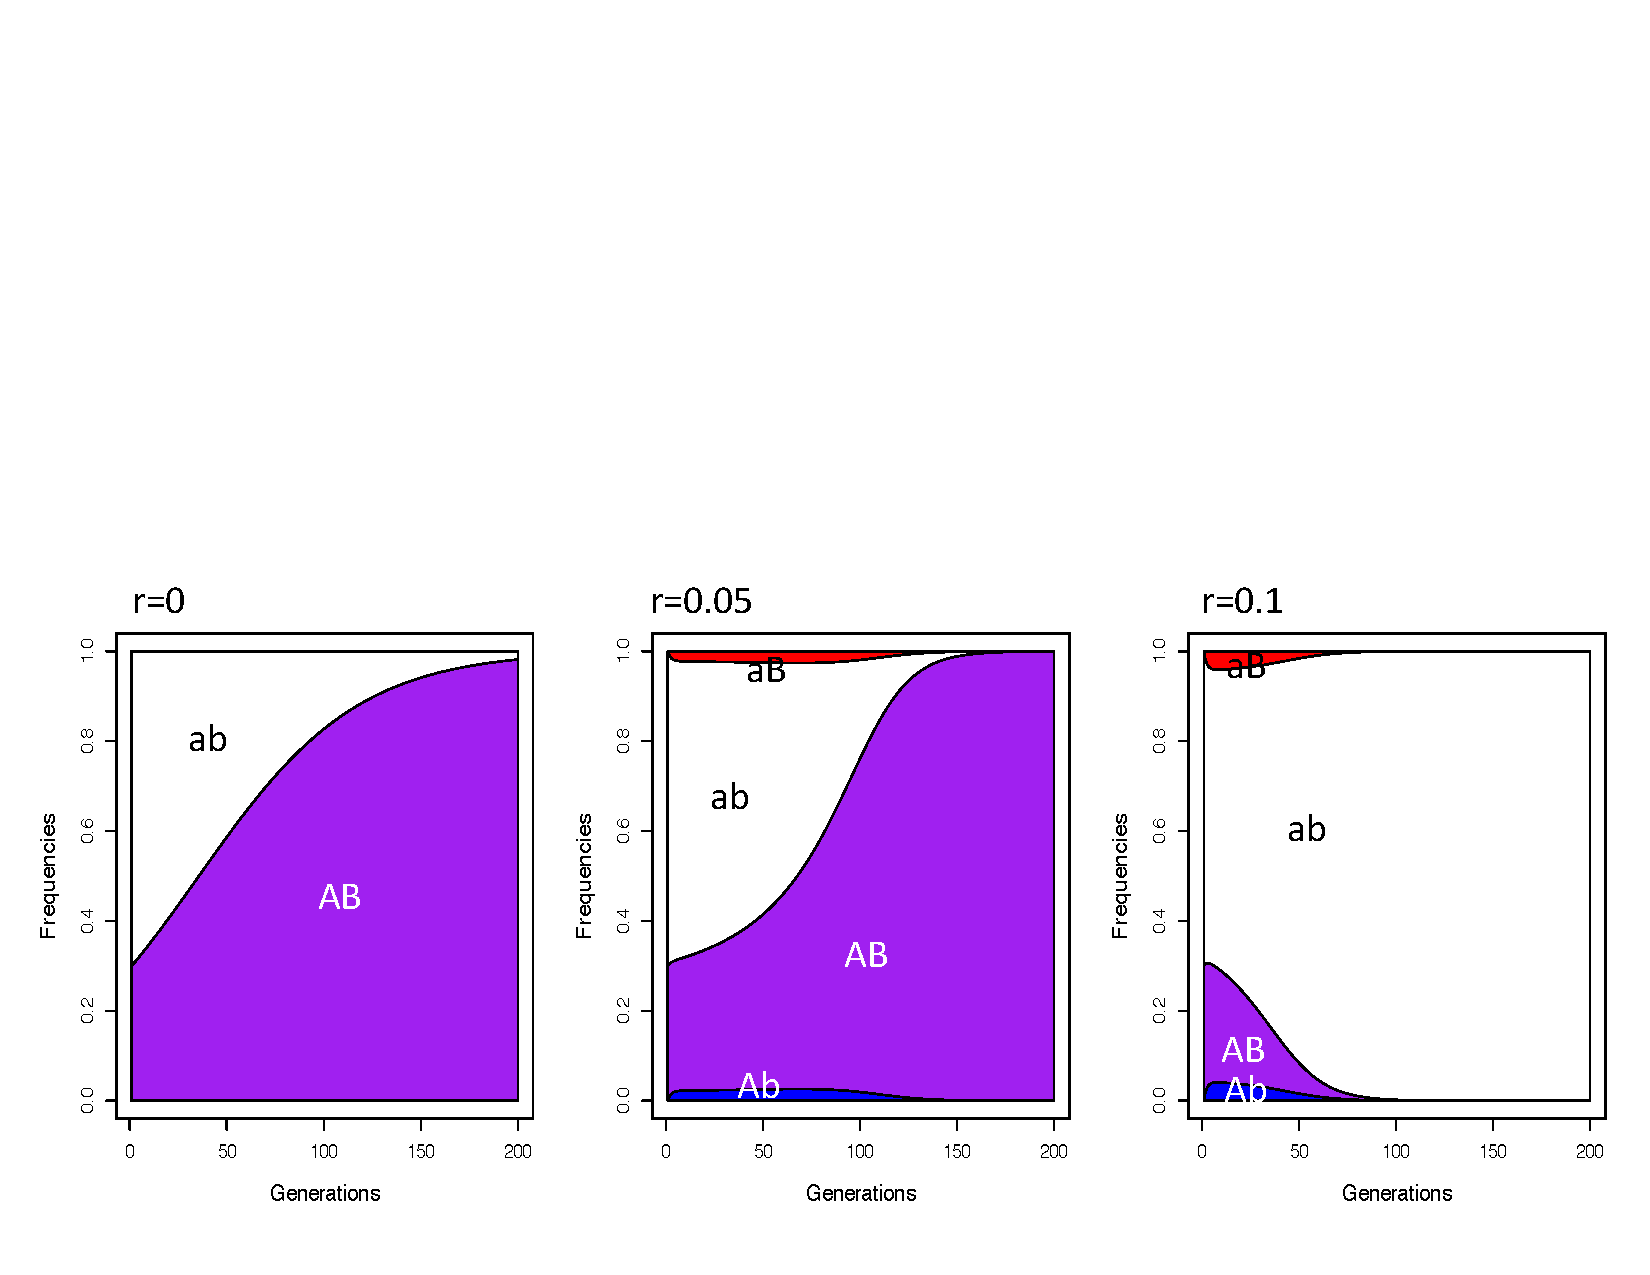
\includegraphics[width = \textwidth]{figures/Epistasis_vs_recom.pdf}
\end{center}
\caption{\gitcode{https://github.com/cooplab/popgen-notes/blob/master/Rcode/two_locus_sel.R}} \label{fig Epistasis_vs_recom}  
\end{figure}

The haplotype AB can spread from low frequency if recombination doesn't break it apart at too high a rate. When recombination rates are higher, recombination prevents either the A or the B allele from spreading because recombination swops the A allele from the B background onto the b background, where it suffers low fitness (and similarly for the B allele). The ab haplotype doesn't suffer the same consequence because it is in the majority, so when recombination occurs the a allele is usually recombined back on to the b background with no consequence. Thus recombination can prevent the spread of beneficial epistatic combinations of alleles. We'll look into this more when we discuss the evolution of recombination suppressors in Section \ref{epistasis_inversion}.

\subsection{Muller's ratchet}

\begin{marginfigure}[-3cm]
\begin{center}
  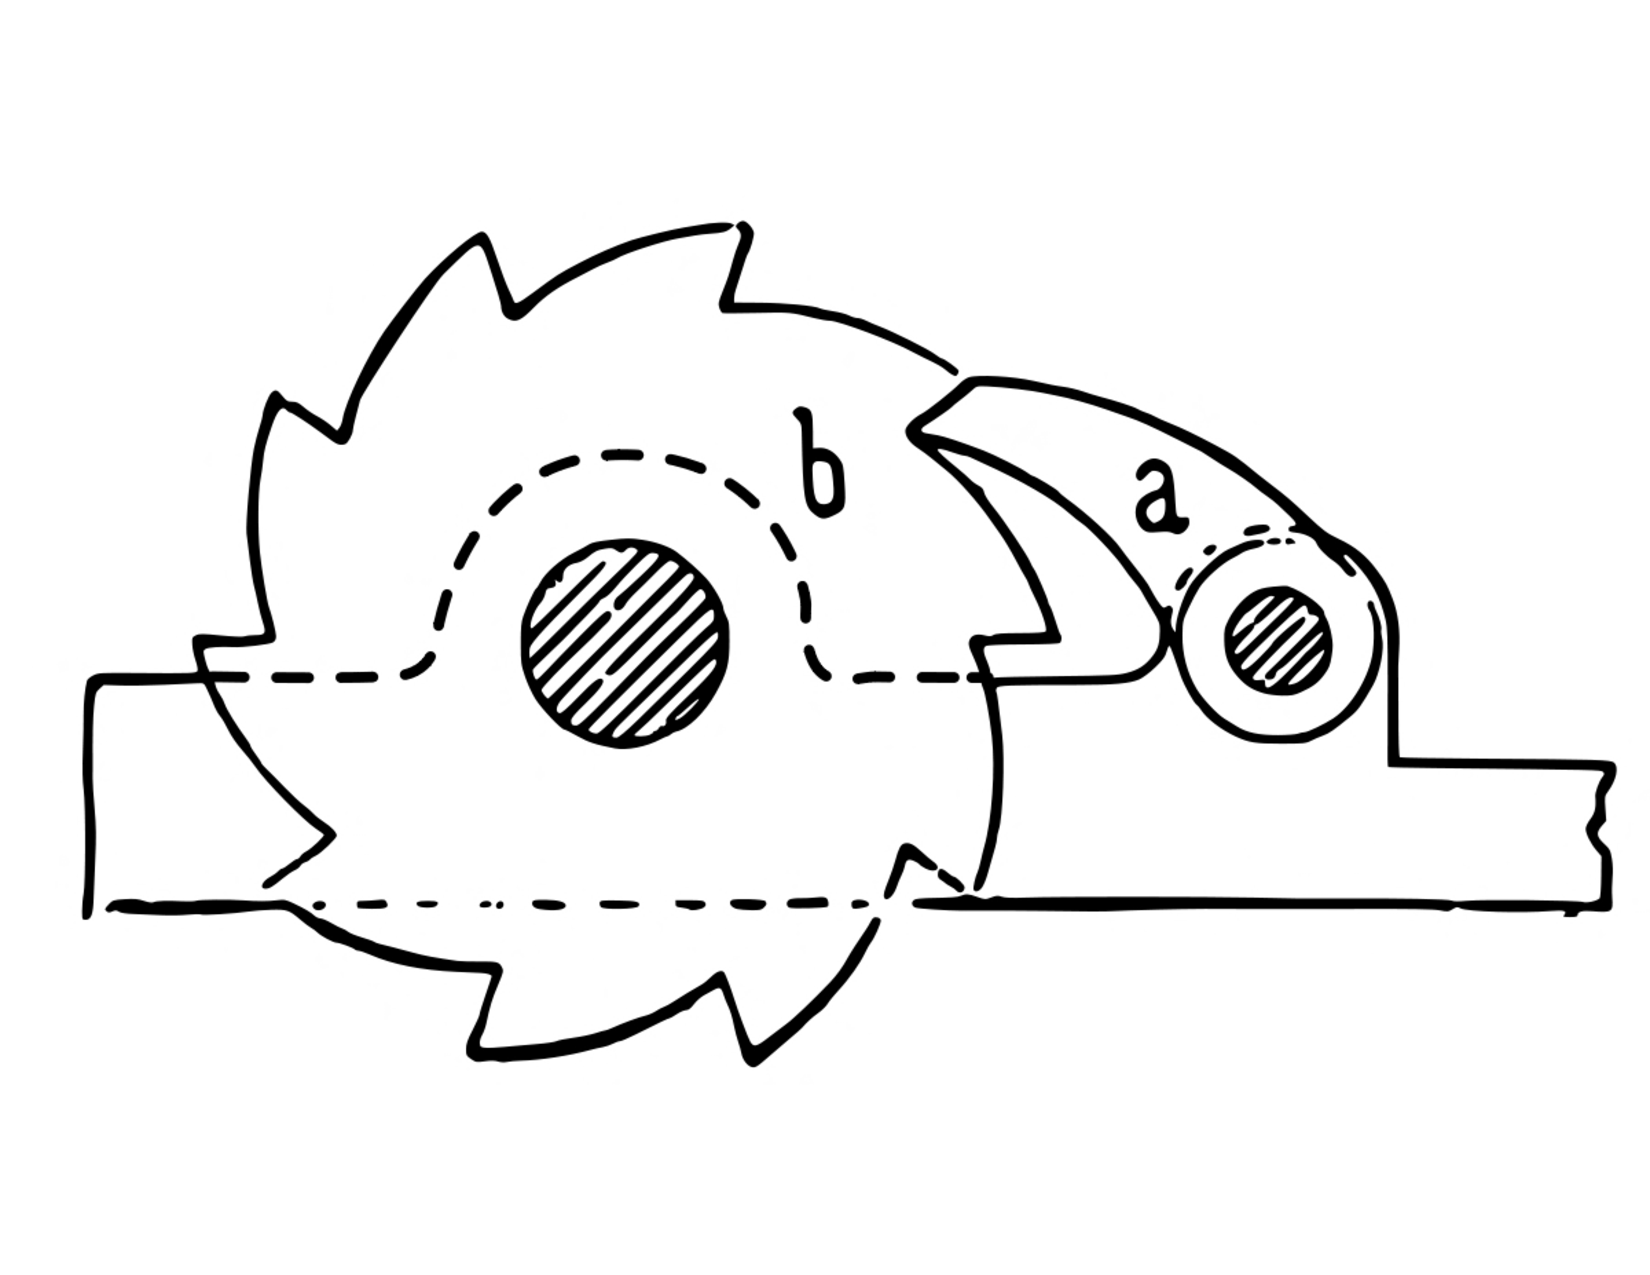
\includegraphics[width = 0.75 \textwidth]{illustration_images/multiple_sel_loci/ratchet/1200px-Sperrklinke_Schema.pdf}
\end{center}
\caption{A Ratchet. A cog (b)  with asymmetric teeth that can only turn one way as the pawl (a) prevents it turning the other way. \newline \noindent \tiny{Original sketch from Brockhaus Konversations-Lexikon, Vol. 10, 1894, page 420. Georg Wiora (reworked by Dr. Schorsch). From \href{https://commons.wikimedia.org/wiki/File:Sperrklinke\_Schema.jp2}{wikimedia}. Licensed under CC
    BY-2.0 } } \label{Fig:Ratchet}  
\end{marginfigure}
There is a constant influx of deleterious mutations along any chromosome (red alleles in Figure \ref{Fig:Mullers_Ratchet}). In asexual populations, or regions of the genome lacking recombination, this leads to nearly inevitable decrease in fitness due to the loss of high fitness haplotypes a process known as `Muller's ratchet' \citep{muller1964relation}.

Different haplotypes vary in the number of deleterious alleles they carry. The haplotypes carrying the most deleterious alleles can be lost by drift, and by selection acting against them, but haplotypes carrying high numbers of deleterious alleles are easily recreated by new mutations. The converse can also happen, if the selection against these each deleterious alleles is relatively weak, the population can accidentally lose the haplotype carrying the least number of deleterious alleles (middle panel of Figure \ref{Fig:Mullers_Ratchet}). \begin{marginfigure}[0cm]
\begin{center}
  \includegraphics[width = \textwidth]{figures/Mullers_Ratchet.pdf}
\end{center}
\caption{A cartoon of haplotypes at three time points showing the action of Muller's ratchet in an asexual population.} \label{Fig:Mullers_Ratchet}  
\end{marginfigure} Once we have lost this haplotype it is hard to recreate, as that would require unlikely back mutations to remove the deleterious mutations from the population. After the the loss of the least deleterious haplotype, we have ratcheted up the mean deleterious mutations in the population and ratcheted down the mean fitness of the population. This will keep happening, by chance we can keep losing the haplotype with fewest deleterious alleles (bottom left panel of Figure \ref{Fig:Mullers_Ratchet}). Thus number of deleterious alleles carried in our asexual population will gradually increase. This may eventually doom asexual population to extinction, as their mean fitness declines over time.

In a sexual population, the same process can start. We can lose by chance the haplotype with the fewest deleterious mutations (middle right panel of Figure \ref{Fig:Mullers_Ratchet}). However, recombination among deleterious haplotypes can recreate this haplotype carrying few deleterious alleles. Such a crossover is shown as a red X in the middle right panel of  Figure \ref{Fig:Mullers_Ratchet}, and the resulting recombinant haplotype few of deleterious is shown in the lower right panel. Therefore, Muller's ratchet doesn't tick forward in sexual populations, as even a small amount of recombination is enough to stop its progression.  
\subsection{An example of the costs of asexuality.}

\begin{marginfigure}[0cm]
\begin{center}
  \includegraphics[width = \textwidth]{figures/Reciprocal_translocations_Hollister.pdf}
\end{center}
\caption{A schematic diagram of the karotype of an evening primrose. The two columns show a heterozygote individual's diploid chromosomal complement. Each chromosome is heterozygote for two different translocations. For example both the top-most chromosomes has one arm from chromosome 1, but the other arm is heterozygote for a large translocation from the ancestral chromsome 2 and 10. Due to these translocations the meiotic pairing form a complete ring of chromosomes, which prevent crossing over and independent segregation. Thanks to Jesse Hollister for this image. } \label{Fig:Reciprocal_translocation}  %é
\end{marginfigure}

In the Evening primrose genus ({\it Oenothera}), there are a number of young, independently-derived, asexual species. In each species this asexuality is due to a complicated series of reciprocal translocations, Figure \ref{Fig:Reciprocal_translocation} which prevent recombination and segregation and ensure that every plant is permanently-heterozygote for these rearrangements due to lethality. This system is quite complicated, and super cool. We don't need to worry about the details but importantly each species is functionally asexual. \citet{hollister2014recurrent} sampled transcriptome data from across the Evening primrose clade, and took advantage of 7 independent, asexual-sexual sister pairs of species to examine the impact of the evolution of asexuality for molecular evolution.  
\begin{figure}
\begin{center}
  \includegraphics[width = 0.8 \textwidth]{Journal_figs/recom_selection/evening_primrose/evening_primrose_omega.pdf}
\end{center}
\caption[][4cm]{$\dNdS$ calculated on sexual (circles) and asexual (diamonds) lineages of each of seven sister pairs of species. Data from \citet{hollister2014recurrent}. \gitcode{https://github.com/cooplab/popgen-notes/blob/master/Journal_figs/recom_selection/evening_primrose/evening_primrose_omega.R}| } \label{fig:evening_primrose_omega}  %é
\end{figure}

The $\dNdS$ for the sexual and asexual species for each of the seven pairs (C1-C7) is shown in Figure \ref{fig:evening_primrose_omega}. In every pair $\dNdS$ is higher in the asexual species. The genomes of the asexual species are evolving in a less constrained fashion, likely due to weakly deleterious mutations accumulating due to hitchhiking with beneficial alleles and the slow crank of Muller's ratchet. 
\begin{marginfigure}[0cm]
\begin{center}
  \includegraphics[width = \textwidth]{illustration_images/multiple_sel_loci/Evening_primrose/10575005313_f2c8839a80_k.jpg}
\end{center}
\caption{ Showy evening primrose ({\it Oenothera speciosa}), the sexual species in the clade C2 from Figure \ref{fig:evening_primrose_omega}. \BHLCC{Favourite flowers of garden and greenhouse (1896). Step, E. }{https://www.flickr.com/photos/61021753@N02/10575005313/}{Missouri Botanical Garden}{2.0} } \label{fig:Oenothera}  %é
\end{marginfigure}

\subsection{The maintenance of combinations of alleles in the face of recombination.} \label{epistasis_inversion}

In some cases balancing selection may be attempting to maintain multiple combinations of alleles in the population that work well together. However, recombination may be constantly ripping those alleles away from each other making it difficult to maintain these alleles. This can select for the suppression of recombination. Some of the most dramatic demonstrations of this tension involve the evolution of so-called super genes. We'll first consider the evolution of a mimicry supergene in {\it Heliconius numata} as an example of these dynamics.  

Some of the most spectacular examples of M{\"u}llerian mimicry in the world are found in {\it Heliconius} butterflies. These butterflies are unpalatable to predators, and different species mimic each other so benefiting from not being eaten by predators, which rapidly learn to avoid all these species). In many of these species multiple mimicry morphs are found as we move across geographic space. In  {\it Heliconius numata} a number of different morphs mimic morphs from a distantly related {\it Melinaea} species, see Figure \ref{fig:H_numata}.

\begin{figure} %[0cm]
\begin{center}
  \includegraphics[width = \textwidth]{Journal_figs/recom_selection/H_numata/H_numata.pdf}
\end{center}
\caption{Five sympatric forms of {\it H. numata} from northern Peru, and their distantly related comimetic Melinaea species.  First row: {\it M. menophilus ssp. nov., M. ludovica ludovica, M. marsaeus rileyi, M. marsaeus mothone, and M. marsaeus phasiana}. Second row, {\it H. n. f. tarapotensis, H. n. f. silvana, H. n.f. aurora, H. n.f. bicoloratus, and H. n. f. arcuella}. Figure and caption from \citet{joron2006conserved} cropped, \PLOSccBY. } \label{fig:H_numata}  %é
\end{figure}

To keep things relatively simple lets focus on two differences between  {\it silvana} and {\it  bicoloratus}, the yellow stripe on the top wing of {\it silvana} and the black bottom wing of  {\it  bicoloratus}. Lets imagine that these two differences are due to a simple two locus system (see left column of Figure \ref{fig:numata_two_loc_freqs}). The first locus segregates for Y/y, where the Y allele encodes for a top-wing yellow band, and y encodes for the absence of the yellow band. The second locus segregates for B/b where B encodes for the bottom-wing being black, and b for the absence of black on the bottom wing. If Y is recessive and B is dominant, then the silvana phenotype corresponds to a YY bb genotype. Due to the dominance of the y and B alleles the bicoloratus phenotype can be achieved by various genotypes (Yy Bb, yy BB, Yy BB, yy Bb).  Lets assume that both of these phenotypes offer an advantage as they mimic a {\it M. menophilus} model. But there are also genotypes that don't do as well; YY BB individuals have a yellow band and a black bottom and so don't do a great job mimicking anything and so will be eaten. Thinking about the  four possible haplotypes, y-B has high marginal fitness as due to its combo of dominant alleles it'll always produce a bicoloratus phenotype. Likewise the Y-b haplotype has high marginal fitness, as it does well in the homozygous state ({\it silvana} phenotype), and when it is paired with the y-B allele. However, the Y-B and y-b haplotypes fair less well as they carry two alleles that don't work well with each other and so are often individuals who suffer high rates of predation. 

\begin{figure} %[0cm]
\begin{center}
 \includegraphics[width = \textwidth]{figures/selection_recom_interaction/H_numata_two_loc_freqs.pdf}
\end{center}
\caption{Left column a hypothetical two locus model to describe the {\it H. numata} {\it silvana} and {\it  bicoloratus} morphs.. Right column the frequency dynamics of the four haplotypes under two different recombination regimes. The model has negative frequency dependent selection acting to increase the frequency of the mimicry morph that is rarer in the population. While all individuals with genotypes corresponding to a mixed phenotype, e.g. YY BB, have very low fitness as they mimic no Melinaea and so are quickly eaten.   Butterflies cropped from \citet{joron2006conserved} cropped, \PLOSccBY, \gitcode{https://github.com/cooplab/popgen-notes/blob/master/Rcode/two_locus_sel.R} } \label{fig:numata_two_loc_freqs}  %é
\end{figure}

If no recombination occurs between these loci ($r=0$, Figure \ref{fig:numata_two_loc_freqs}), then the Y-B and y-b are selected out of the population, and the y-B and and  Y-b can be stably maintained. However, when there's too much recombination between our loci (e.g. $r=0.4$, Figure \ref{fig:numata_two_loc_freqs}) the high-fitness haplotypes keep getting ripped apart by recombination and the Y-b is lost from the population as it's recessive advantage is lost as it's too often being broken up by recombination in heterozygotes.

\marginnote{\begin{quote}
``coadapted combinations of several or many genes locked in inverted sections of chromosomes and therefore inherited as single units.''
\citet{dobzhansky1970genetics} on supergenes. 
\end{quote} }
\subsection{Supergenes to the rescue!} \label{Section:super_genes}

So our polymorphisms can only be maintained if they are tightly linked, i.e if these alleles arose at loci that are genetically close to each other. But how is it possible that these alleles arose close to each other? Well the trick is that they don't necessarily have to arise very close to each other. If such a system is polymorphic but being regularly broken up by recombination, a chromosomal inversion--the flipping around of a whole section of chromosome-- can arise and will suppress recombination. Imagine that our two loci are far apart genetically, and a chromosomal inversion arises on the Y-b  background forming the b-Y haplotype. This inverted haplotype will not recombine with the y-B haplotype when it is present in a heterozygote, thus it is not broken down by recombination. This inverted haplotype, which enjoys the fitness benefits of the Y-b, can therefore replace the Y-b haplotype in the population. The two other low fitness haplotypes will disappear as they sre no longer being generated by recombination, leaving just the y-B and b-Y. 
  The polymorphism system now behaves like alleles at a single locus, a super gene  (e.g. like $r=0$ in Figure \ref{fig:numata_two_loc_freqs}).

  Now the {\it H. numata} system is vastly more complicated than our toy two locus system, presumably involving many changes and refinements, but the same principle holds \citep{joron2011chromosomal}. The differences between the different {\it H. numata} mimmicy morphs is found on a single chromosome, and the inheritance behaves as if controlled by a single locus (albeit with many alleles).  The {\it H. n. f. silvana} individuals carry a recessive haplotype of alleles that which is known to be locked together by a $\sim 400$kb inversion, that is a different chromosomal orientation from the {\it bicoloratus} allele (haplotype) which acts as a dominant allele. Other alleles at this same chromosomal region provide the genetic basis of the other morphs, and sometimes correspond to further inversions with a range of dominance relationships. 


\begin{figure} %[0cm]
\begin{center}
\includegraphics[width = \textwidth]{Journal_figs/recom_selection/Mimulus_inversion/annual_perennial_fitness.pdf}
\end{center}
\caption[][-2cm]{{\bf Left)} A coastal perennial and an Inland annuals {\it Mimulus gutatus} \citet{lowry2010widespread}, image from \citet{lowry2010widespread} \PLOSccBY. {\bf Right)} A reciprocal transplant experiment showing that coastal perennial and an Inland annuals are locally adapted to their respective habitats. Data from  \citet{lowry2010widespread}, \gitcode{https://github.com/cooplab/popgen-notes/blob/master/Journal_figs/recom_selection/Mimulus_inversion/annual_perennial_fitness.R}. 
}\label{fig:annual_perennial_fitness}
\end{figure}


\paragraph{Local Adaptation, Speciation, and Inversions.}
\begin{marginfigure} %[0cm]
\begin{center}
\includegraphics[width = \textwidth]{figures/inversion_mig_sel_balance.pdf}
\end{center}
\caption{A two locus, two population migration-selection balance system. Two loci A and B segregate for an Inland and Coastal adapted alleles.} \label{two_locus_mig}
\end{marginfigure}
Inversions have long been thought to play an important role in local adaptation and speciation.
One example of an inversion underlying local adaptation occurs in {\it Mimulus gutatus},  in Western North America, where there are annual and perennial ecomorphs with very different life history strategies (see Figure \ref{fig:annual_perennial_fitness}). The perennial form grows in many places along the Pacific coast, and in other places with year around moisture; it invests a lot of resources in
achieving large size and laying down resources for the next year, and as a result flowers late. The annual form grows inland, e.g. the California central valley,
where it has to invest all its effort in flowering rapidly before the long, hot, dry summer. Neither ecomorph does well in the other's environment. The perennials get crisped
before they have a chance to flower, while the annuals suffer from high rates of herbivory and cannot tolerate the salt spray.
\citet{lowry2010widespread} found that large inversion controled a lot of of the phenotypic variation in
flowering time and a range of other morphological differences between these two morphs. They also showed that the inversion controled a reasonable proportion of the
differences in fitness in the field, consistent with it underlying the fitness tradeoffs involved in local adaptation.

Why would an inversion be involved in locking together local adapted alleles? The basic idea, like above, is an inversion can be selected for we have two (or more) loci segregating for locally adapted alleles (Figure \ref{two_locus_mig}). Locally advantagous haplotypes are in danger of being broken up by recombination with maladapted haplotypes, which are constantly being
introduced into each population by migration from the other. If an inversion arises that locks these alleles together in one population, it can be selected for as does not suffer the ill effects from recombination with migrating maladaptive haplotype. 
 
  % In this simple model of viability selection
\begin{figure*} %[0cm]
\begin{center}
\includegraphics[width = \textwidth]{Journal_figs/recom_selection/Sex_determ_why_so_many_ways/Tree_of_sex.png}
\end{center}
\caption{Diversity of sex determination systems for representative plant and animal clades. Figure and caption from \citet{bachtrog2014sex}, \PLOSccBY. }  \label{fig:Tree_of_sex}
\end{figure*}
\subsection{Sex Chromosomes and the dynamics of selection and recombination.}

The evolution of sex chromosomes and new systems of genetic sex determination provide a beautiful demonstration of the interplay of selection and recombination. But first it's worth taking a step back and thinking the difference between an species being sexual, having male and female gametes, and having separate sexes (i.e. males and females), and the mechanisms for determining the sexes. Many species are sexual but with no separate sexes or even male or female gametes. The production of different sized gametes (anisogamy) has arisen a number of times in multi-cellular life, with male and female gametes are defined by their relative sizes. The smaller, and often more mobile, gametes are defined male gametes  (e.g. sperm), while the larger, well provisioned, and often less mobile are defined as female gametes (e.g. egg cell). The evolution of anisogamy is thought to be due to disruptive selection due to a tradeoff pulling in opposite directions towards mobile gametes able to move further and in the opposite direction towards better provisioned gametes better able to build larger zygotes. In many organisms individuals can produce both male and female gametes, while some species have evolved separate sexes, likely in part as an inbreeding avoidance mechanism.There is huge diversity in sex determination mechanisms across the eukaryotic tree (Figure \ref{fig:Tree_of_sex}. This is all to say, that biology is wonderfully diverse and complicated.
  \begin{marginfigure}[-3cm]
\begin{center}
\includegraphics[width = \textwidth]{illustration_images/multiple_sel_loci/volvox/volvox.jpg}
\end{center}
\caption{ {\it Volvox aureus}, Volvox are spherical, multicellular green algae. The surface is made up of a single layer of somatic cells (up to 50k cells) beating their flagella. Some species of Volvox have individuals with both male and female gametes, being made here in the germ cells (a and g respectively) in the middle of the sphere. Some Volvox have separate sexes, where different individuals produce male and female gametes.}
\end{marginfigure}
In mammals, and many other systems with genetic sex determination, the genes responsible for sex determination lie on a pair of heteromorphic sex chromosomes, i.e. pair of chromosomes that are quite different in size. In mammals where most males are XY and females XY. Where the male determining Y chromosome that has a very small gene content compared to the X chromosome. But in other groups such as birds, and some snakes, sex determination is a ZW system with females being ZW and males being ZZ. In those systems females carry a gene poor W with males being the homogametic sex, carrying two Zs.  If you are still reading send Graham a picture of Nettie Stevens, she discovered sex chromosomes in 1905 \citep{stevens1905studies}. These examples of heteromorphic sex chromosomes, and many others like them, are thought to have arisen from an ancestral pair of autosomes? What then explains their evolution? %The Y chromosome does not recombine over most its length with the X, and so most of the

 \begin{marginfigure} %[0cm]
\begin{center}
\includegraphics[width = \textwidth]{figures/neo_Y_evol.pdf}
\end{center}
\caption{A cartoon of formation of a neo-Y chromosome and subsequent suppression of recombination. A pair of orthologous automosomes is shown in the top most panel.  Sexually-antagonistic male-beneficial, female-detrimental alleles are shown as vertical lines. A newly arising dominant, male-determining allele is shown as a blue circle. The inversions are shown as brackets. The non-recombining region linked to the sex determining allele coloured red.}  \label{fig:neo_Y_evol}
% sex symbols from https://commons.wikimedia.org/wiki/File:Gender_symbols_side_by_side_solid.svg
\end{marginfigure}

One broad explanation for the evolution of sex chromosome is illustrated in Figure \ref{fig:neo_Y_evol} and goes as follows:\\
\begin{enumerate}
\item There are a pair of ancestral autosomes with sexually-antagonistic male-beneficial, female-detrimental alleles segregating on them (the converse can occur but arent central to the evolution of Y chromosomes). These alleles can persist in the population for some time but are eventually lost due to their cost in females. 
\item A dominant, male-determining allele arises on one of the chromosomes. Let's call this chromosome our proto-Y and the other our proto-X. All individuals who are heterozygous for the Proto-Y will be male, individuals who are homozygous for the proto-X. No individuals will be homozygous for the proto-Y, as individuals can receive at most one Proto-Y, that of their father. 
\item Our sexually-antagonistic alleles benefit from being on the same chromosome as our male-determining allele as then they are guaranteed to be in males. However, if they recombine off the proto-Y on to the proto-X they are at a disadvantage.
\item If an inversion arises on the background of the proto-Y chromosome it can lock together the male-determining allele and some of our sexually-antagonistic alleles. This inversion can initially spread as gains the benefit of the sexually-antagonistic alleles without the cost of recombination. This inversion can't spread to fixation as Fisherian selection on the sex ratio keeps it in check.
\item Further inversions can potentially cement additional sexually-antagonistic alleles into tight linkage with the male-determining allele.
\end{enumerate}
Sex chromosomes, under this hypothesis, are super genes locking together sex determination and sexually-antagonistic alleles. Our male-beneficial, female-detrimental alleles work well on the background of the male-determining allele and poorly off it, that's exactly the supergene setup we encountered in Section \ref{Section:super_genes}. This sketch can be flipped to describe the evolution of ZY systems. 


\begin{figure} %[0cm]
\begin{center}
\includegraphics[width = \textwidth]{figures/selection_recom_interaction/Cichlid_OB_sex_linkage.pdf}
\end{center}
\caption{The sex-specific effects of the OB allele.  \newline \noindent \tiny{Image credits: Blue mbuna Male  {\it L. fuelleborni} by \href{https://commons.wikimedia.org/wiki/File:Labeotropheus_fuelleborni_in_Botanic_garden_in_Teplice_(2).JPG}{Chmee2}; % ( {\it Labeotropheus fuelleborni}).
  OB  Male {\it L. fuelleborni} by \href{https://de.wikipedia.org/wiki/Schabemund-Buntbarsch\#/media/File:Labeotropheus_fuelleborni_01.jpg}{Doronenko};
  Brown ob  {\it Tropheops} female by \href{https://www.flickr.com/photos/52993488@N03/4890217915}{Alexandra Tyers};
  Female  {\it L. fuelleborni} orange morph,  by \href{https://commons.wikimedia.org/wiki/File:Labeotropheus_fuelleborni1.jpg}{Mikko Stenberg} 
}}
\end{figure}

A colourful example of the initial conditions for the evolution of a novel sex determination system is offered in lake Malawi there are many very closely related cichlids species \citep{roberts2009sexual}. In many of these species the males are brightly coloured to attracted females, while the females are often brown to help them avoid predators. In some of these species there is an alternative orange morph, called the marmalade cat morph, which are cryptic against the rocky bottom of the lake. This morph is due to a dominant \graham{double check} mutation called OB at the pax7, and the allele appears to shared across many of these species. This OB allele works well in females, however, in the males the OB allele disrupts their bright colouration. Thus the OB polymorphism is sexually antagonistic, i.e. it works well in females and poorly in males.

Males carrying the male-deleterious OB allele are rarely found, despite the allele being common in females. Why is that? Well because the OB allele is tightly linked to a newly emerged female-determining allele (W), with males carrying two copies of the Z allele. Males usually are homozygous for the ob-Z haplotype, while females can being either orange (OB-W/ob-Z) or brown (ob-W/ob-Z). Recombination between these two loci seems to be very rare, and so the sexually antagonistic allele OB appears to be mainly female specific. Thus the spread of this sex determining allele has potentially helped resolve sexually-antagonism while it aided its own spread. An inversion on the Z background would lock together these two alleles, and spread.  

\paragraph{The degradation of heterogametic sex chromosomes.} 
Our inversions on the neo-Y chromosome have created a issue (or conversely the neo-W in ZW systems). The inverted block, containing the male-determining allele, is now inherited as a non-recombining haplotype. Why's that?  Well the inversion doesn't recombine in heterozygotes, and the neo-Y inversion region is only ever found in heterozygote males.\sidenote{This differs from the situation that most other non-sex chromosome inversions find themselves in as they homozygous some of the time and so experience recombination.} Thus the region of chromosome tied up within inversions is effectively asexual and subject to many of the issues that come along with that. The hitchhiking of deleterious alleles will be common and Muller's Rachet will begin to tick. Many mildly deleterious alleles will be allowed to fix through these mechanisms, leading to the accumulation of permature stop codons and silencing mutations in non-essential genes within the neo-Y inversion. The X chomosome will maintain copies of these genes, and sometimes the expression of these genes will have to be up-regulated in males to accommodate for the degradation of the Y based copy leading to lower dosage of these genes.\sidenote{Indeed in some heterogametic sex chromosome systems there are evolved dosage compensation systems that deal specifically with these issues. }  Transposable elements can also accumulate on the non-recombining section of the Y chromosome, some times in huge numbers, as the purging of these transposable elements will be inefficient in this region.  But there's little to stop the non-recombining section of neo-Y chromosome from expanding more due to the short-sighted selection for inversions that further tie up sexually-antagonistic alleles. Our non-recombining section of the Y chromosome maybe expanding to occupy more of the chromosome, as it is losing functional genes and bloating up with repeative DNA. Eventually much of what remains may be genes that are essential to male function, as is the case with old Y chromosomes such as humans. 

%How quickly can this happen? 
 
% https://journals.plos.org/plosbiology/article?id=10.1371/journal.pbio.1001643


\bibliography{

\end{document}
